\documentclass[10pt, twoside, openright]{book}

% https://tex.stackexchange.com/questions/14008/how-to-put-a-line-break-in-section-heading
% https://tex.stackexchange.com/questions/268975/arcs-in-linguistic-functional-structure-lfg

\usepackage[T1]{fontenc}
%\usepackage{fontspec}
\usepackage{newtxtext}
\usepackage{inconsolata}
\usepackage{graphicx}
\usepackage{fancyhdr}
\usepackage{sectsty}
\usepackage{listings}
\usepackage{url}
\usepackage{float}
\usepackage{dpfloat}% double pane floats
\usepackage[fit]{truncate}
\usepackage{multirow}
\usepackage{array}
\usepackage{template/lic_bok}
\usepackage{pdfpages}
\usepackage{tikz}
\usepackage{tikzpagenodes}
\usepackage{forest}
%\usepackage[nooneline]{subfigure}
\usepackage{wrapfig}
\usepackage{multicol}
\usepackage{colortbl}
\usepackage{capt-of}% captionof
\usepackage{extendj}

%\usepackage{showframe}% layout debug

\usepackage[b5paper]{geometry}
% Page margins:
\geometry{
  inner=24mm,
  outer=24mm,
  top=20mm,
  bottom=36mm,
  bindingoffset=10mm,
  headheight=10mm
}

%\setsansfont{Nimbus Sans L}

%\setsansfont{Nimbus}[
%  Path=fonts/,
%  BoldFont=*-Bold,
%  Extension=.otf
%]

%\setmonofont{Inconsolata}[
%  Path=fonts/,
%  UprightFont=*-Regular,
%  BoldFont=*-Bold,
%  Extension=.ttf
%]

\usepackage{titling}% \theauthor, \thetitle

% Custom quote environment:
\usepackage{setspace}
\usepackage{etoolbox}
\AtBeginEnvironment{quote}{\singlespacing\small}

\usepackage{mathtools}

\usepackage[flushleft]{threeparttable}

% Corags dependencies:
\usepackage{algorithm}
\usepackage{algpseudocode}
\usepackage{amssymb,amsmath,amsthm}

\allowdisplaybreaks % Allow page breaks in align.

% Multiplicities dependencies:
\usepackage{booktabs}
\usepackage[hidelinks]{hyperref}
%\usepackage{xltxtra}
\usepackage{textcomp}% trademark symbol
\usepackage{makecell}% diagonal in table cell
\usepackage{fancybox}
\usepackage{color}
\usepackage{adjustbox}
\usepackage{xcolor}

% Wavy underline for Paper II.
\usepackage{ulem}
\normalem % get normal emphasis back

% Test selection:
%\usepackage[noend]{algpseudocode}

\usetikzlibrary{
arrows.meta,
chains,
%quotes, % Text above arrows.
scopes,
shapes,
backgrounds,
patterns,
shadows,
decorations,
decorations.text,
decorations.pathmorphing % snakes
}

% Inline verbatim in multiplicities:
\def\inline{\lstinline[basicstyle=\sffamily,keywordstyle={}]}

\usepackage[backend=biber,
maxcitenames=2,
mincrossrefs=99,
style=alphabetic,
doi=false,
isbn=false,
url=false,
refsegment=chapter,
defernumbers=true,
sorting=nyt]{biblatex}
% https://tex.stackexchange.com/questions/187643/biblatex-how-can-i-suppress-some-fields-for-multiple-entry-types
%\AtEveryBibitem{%
%\clearfield{editor}%
%}
\addbibresource{refs.bib}
\addbibresource{papers/corags.bib}
\addbibresource{papers/java7.bib}
\addbibresource{papers/multiplicities.bib}
\defbibheading{subbibliography}{\addcontentsline{toc}{section}{References}\section*{References}}

\newsavebox{\lstboxleft}
\newsavebox{\lstboxright}

\forestset{
  default preamble={
    for tree={
      draw,
      ellipse,
      font=\rmfamily\slshape,
    }
  }
}

\tikzset{
  attribute/.style={
    draw,
    rectangle,
    rounded corners,
    fill=white!80!gray,
    font=\footnotesize\itshape
  },
  % Edge label style for trees (forest):
  edgelbl/.style={midway, anchor=south, sloped, auto=false, font=\footnotesize\itshape}
}

\hyphenation{in-stru-men-ta-tion}
\hyphenation{Jast-Add}
\hyphenation{CEval}

% Multiplicities
\hyphenation{sym-bol-ic}
\hyphenation{ob-ject}
\hyphenation{re-ified}
\hyphenation{syn-chro-nized}
\hyphenation{Jast-Add-J}

% Popvet
\hyphenation{a-na-lys}
\hyphenation{a-na-lys-er}
\hyphenation{a-na-lys-era}


\newtheorem{observation}{Observation}
\newtheorem{definition}{Definition}
\newtheorem{theorem}{Theorem}
\newtheorem{lemma}{Lemma}

% JastAdd code listings
\newcommand{\figcodesize}{\fontsize{8pt}{8pt}}
\newcommand{\codesize}{\fontsize{8pt}{8pt}}
\newcommand\figcodestart{\vspace*{-5pt}}
\lstdefinelanguage{jastadd}
{
  morekeywords = {
    % JastAdd
    syn, inh, eq, ast,
    coll, with, contributes, to, when, root, then,
    nta, circular, lazy,
    rewrite,
    % Java
    package, import,
    class, extends, boolean, false, true,
    final,
    while, do, for, each, if, else, switch, case, default,
    this, abstract, void, new, return, null,
    try, catch, throw, finally, public, aspect, implements,
    interface, protected, int, long, char, super,
    % annotations
    @Parallel, @Override,
    % python
    def, True, False,
    % C++
    bool, auto
  },
  otherkeywords = { ::=, *, <, >, :, [, ], ?, =},
  sensitive = true,
  escapeinside={/+}{+/},
}

\lstset{language=jastadd,
  basicstyle=\ttfamily,
  keywordstyle=\bfseries,
  morekeywords={T, nil},
  numbers=none,
  showspaces=false
}

% https://tex.stackexchange.com/questions/11707/how-to-force-output-to-a-left-or-right-page/11709#11709
\newcommand*\cleartoleftpage{%
  \clearpage
  \ifodd\value{page}\hbox{}\newpage\fi
}

\newcommand{\figref}[1]{Figure~\ref{#1}}
\newcommand{\secref}[1]{Section~\ref{#1}}

% Java classes in text
\newcommand{\Class}[1]{\textbf{\texttt{\footnotesize{#1}}}}
\newcommand{\Attr}[1]{\textbf{\texttt{\footnotesize{#1}}}}
\newcommand{\Method}[1]{\textsf{\footnotesize{#1}}}
\newcommand{\Keyword}[1]{\textbf{\texttt{\footnotesize{#1}}}}
\newcommand{\Set}[1]{\textsc{#1}}

% References
\newcommand{\Chapter}[1]{Chapter~\ref{#1}}

\hyphenation{JastAdd}
\hyphenation{IntelliJ}
\hyphenation{JModelica}

% Make all sections sanserif.
\allsectionsfont{\sffamily}

% Make fancy header and no footer.
\pagestyle{fancy}
\renewcommand{\chaptermark}[1]{\markboth{#1}{}}
\renewcommand{\sectionmark}[1]{\markright{\thesection\ #1}}
\fancyhf{}
\fancyhead[LE, RO]{\bfseries\thepage}
\fancyhead[LO]{\itshape \rightmark}
\fancyhead[RE]{\truncate{.95\headwidth}{\itshape \leftmark}}
\renewcommand{\headrulewidth}{0.5pt}
\renewcommand{\footrulewidth}{0pt}%
\setlength{\headheight}{75pt}
\fancypagestyle{plain}{
  \fancyfoot[LE, RO]{\chapterFoot}
  \fancyhead{}
  \renewcommand{\headrulewidth}{0pt}
}

\newcommand{\chapterFoot}{}
\newcommand{\markmargin}{}
\newlength{\spiff}

\newif\ifpopvetOnly

\newif\ifpaperI % Java 7
\newif\ifpaperII % Multiplicities
\newif\ifpaperIII % Test Selection
\newif\ifpaperIV % CoRAGs

\paperItrue
\paperIItrue
\paperIIItrue
\paperIVtrue

%\popvetOnlytrue

\newcommand{\paperIref}{%
Jesper Öqvist and Görel Hedin.
``Extending the JastAdd Extensible Java Compiler to Java~7''.
In \emph{Proceedings of the 10th International Conference on Principles and Practicies of
Programming on the Java Platform: Virtual Machines, Languages, and Tools (PPPJ'13), ACM,
pp. 147--152}. Stuttgart, Germany, 2013.
}
\newcommand{\paperIIref}{%
Friedrich Steimann, Jesper Öqvist, and Görel Hedin.
``Multitudes of Objects: First Implementation and Case Study for Java''.
In \emph{Journal of Object Technology, Vol. 13, no. 5 (November 2014), pp. 1:1--33}.
}
\newcommand{\paperIIIref}{%
Jesper Öqvist, Görel Hedin, and Boris Magnusson.
``Extraction-Based Regression Test Selection''
In \emph{Proceedings of the 13th International Conference on Principles and
Practices of Programming on the Java Platform: Virtual Machines, Languages, and Tools (PPPJ'16), ACM,
pp. 5:1--5:10}. Lugano, Switzerland, 2016.
}
\newcommand{\paperIVref}{%
Jesper Öqvist and Görel Hedin.
``Concurrent Circular Reference Attribute Grammars''.
In \emph{Proceedings of the 10th ACM SIGPLAN International Conference on Software Language
Engineering (SLE 2017), pp. 151--162}. Vancouver, BC, Canada, 2017.
}

\title{Contributions to\\
Declarative Implementation of\\
Static Program Analysis}
\author{Jesper {\"O}qvist}
\date{2019}

% Make tex a bit less neurotic:
\sloppy
\raggedbottom

\begin{document}

\ifpopvetOnly
\else
% Title page.
\frontmatter
\begin{titlepage}
{
  \thispagestyle{empty}

  \begin{tikzpicture}[remember picture, overlay, font=\sffamily]
  \node at (current page text area.north east) [
      anchor=north east,
      yshift = -3cm,
      text width = \textwidth,
      inner sep = 0,
      outer sep = 0,
      align = right
    ] (title)
    {\raggedleft\huge\textbf{\thetitle}\\};
  \node[below = 8cm of title,
      text width = \textwidth,
      inner sep = 0,
      outer sep = 0,
      align = right
    ] (author)
    {\raggedleft\huge\textbf{\theauthor}\\};
  \node[below = 1.5cm of author,
      text width = \textwidth,
      inner sep = 0,
      outer sep = 0,
      align = right
    ] (text) {\raggedleft
      \large{}Doctoral Dissertation, \thedate\\[0.4cm]
      \Large{}Department of Computer Science\\[0.1cm]
      Lund University\\
    };
  \node (mid) at ($(author.south east)!0.7!(text.north east)$) {};
  \draw[thick] (mid -| current page.west) -- (mid -| current page.east);
  \node at (mid -| current page text area.west)
    [anchor = west, shift={(-0.5cm, -1cm)}]
    {\scalebox{0.44}{
\includegraphics{template/lomacdsvs.eps}}};
  \end{tikzpicture}
}

\newpage
\thispagestyle{empty}
\begin{flushleft}
\vspace*{\stretch{1}}
Version 1.1-SNAPSHOT\linebreak[2]

Department of Computer Science\\
Lund University\\
Box 118\\
SE-221 00  Lund\\
Sweden\linebreak[2]

Email: \url{jesper.oqvist@cs.lth.se} \linebreak[2]

Typeset using \LaTeX.\\

Printed in Sweden by Tryckeriet i E-huset, Lund, \thedate.\linebreak[2]

\textit{\copyright ~\thedate~\theauthor}
\vspace{10mm}
\end{flushleft}
\end{titlepage}

\newpage
\section*{Abstract}
Programming languages are ever evolving, with new languages being invented to solve new problems,
and old languages being extended to solve old problems in new ways.
With the continued evolution of programming languages, and with new and improved
static program analyses, we need flexible systems for building our static analyses and compilers.
Declarative programming with \emph{Reference Attribute Grammars} (RAGs) is a fruitful approach for
building extensible and maintainable static program analyses and compilers. With declarative programming,
code is easier to write, easier to understand, and easier to extend.
%With RAGs, compilers can be automatically parallelized and easily extended.

This thesis presents contributions to declarative static program analysis implementation with RAGs.
In particular, I have developed new language extensions for the Java programming language,
as well as new static analyses and tools for Java, based on the extensible Java compiler ExtendJ.
Language extensions include an implementation of Java~7, and a new programming mechanism,
\emph{multiplicities}. A new static analysis-based tool presented in this thesis is a
regression test selection tool, which reduces testing time for Java software development.

My contributions also include new design patterns for declaratively specifying static analyses
in RAGs, and significant improvements to the ExtendJ compiler. My work in ExtendJ includes
developing the first version of the compiler with fully declarative static analysis.

This dissertation also includes contributions to RAGs, including new algorithms for concurrent
attribute evaluation with implementation in the JastAdd metacompiler. With these new algorithms,
it is possible to parallelize any RAG-implemented analysis.
In particular, I parallelized static analysis in the ExtendJ compiler
to achieve a twofold speedup and orders of magnitude reduction of latency.


\newpage
\section*{Acknowledgements}

This work was in part funded by the Swedish Research Council under grant 621-2012-4727
and by a 2015 Google Faculty Research Award for supporting concurrent analyses in interactive
programming tools.

This dissertation would not exist if not for Prof. Görel Hedin.
Görel convinced me to start my PhD studies and supervised me along the way.
She told me what to do, corrected my mistakes, and listened to my weird ideas.
I owe Görel my greatest thanks in helping me complete all of this work.

I owe much gratitude to my beloved wife, Elise.  She is the chillest wife, in
the parlance of our times.  Elise kept me sane and healthy while writing this
thesis.  I am also very grateful for our many fun travels and outings during my
time as Ph.D. student.

Thank you Prof. Boris Magnusson for co-supervising me and for the test
selection collaboration.

Thank you Emma Söderberg for co-supervising me, for getting me into running
(\texttt{RuntimeException}), for hosting me at Google for my first internship,
and for many fun collaborations related to JastAdd and other projects during my PhD studies.

Thank you Prof. Friedrich Steimann for the multiplicities collaboration. It was fun to visit
your department in Germany and to work intensely to complete most of the implementation in
a week.

Thank you Niklas Fors, Alfred Åkesson, and Christoff B{\"{u}}rger for collaborations
related to JastAdd development and compiler construction.

For entertaining and enlightening discussions during the time-honored tradition
of fika, I would like to thank
Christoph Reichenbach, Flavius Gruian,
Linus Åkesson, Maj Stenmark, Pierre Moreau,
Jonas Skeppstedt, Gustav Cedersjö, Noric Couderc,
and all of my other colleagues at the computer science department in
Lund, past and present.

Thank you Erik Hogeman for the Java~8 project.

Thank you to all the excellent people whom I had the pleasure to work with at Modelon (Jesper, Jon,
Jonathan, Axel) and Google Mountain View (Ciera, Karl, Valentyn, Hans, Eddie).  Thank you Arun
Chauhan for hosting me during my second internship.

The diagrams in this thesis would not look as nice without a few
essential \LaTeX packages.  Thus, I owe my gratitude to the authors of the
\textsc{PGF}/{\rm Ti\emph{k}Z} packages, and especially Sa\v{s}o
\v{Z}ivanovi\'{c} for developing the excellent \textsc{Forest} package which
I used for drawing all trees in the thesis.

{\singlespacing\footnotesize
I was considering making a list of enemies and placing Måns Magnusson on it for distracting me with
programming problems. However, I finished the thesis on time so I think we can continue to be friends.}


\newpage
\section*{Contribution Statement}

The following papers are included in this dissertation:

\begin{description}
  \item[Paper~I]
    \paperIref
  \item[Paper~II]
    \paperIIref
  \item[Paper~III]
    \paperIIIref
  \item[Paper~IV]
    \paperIVref

    This thesis includes an extended version of this paper, with correctness proofs for the
    algorithms.
    This extended version of the paper was published as a technical report (report number 103,
    Lund University, 2017).
\end{description}

\noindent
The table below indicates the responsibilities Jesper Öqvist had in writing each paper:

\vspace{1em}
\begin{center}
\begin{tabular}{llllll}
  \toprule
  \emph{Paper} & \emph{Writing} & \emph{Concepts} &  \emph{Implementation} & \emph{Evaluation} & \emph{Algorithm} \\
  \midrule
  \textbf{I}    & YES     & YES     & YES & YES & N/A \\
  \textbf{II}   & partial & no      & YES & YES & N/A \\
  \textbf{III}  & yes     & partial & YES & YES & yes \\
  \textbf{IV}   & YES     & YES     & YES & YES & YES \\
  \bottomrule
\end{tabular}
\end{center}
\vspace{1em}

\noindent
Capital letters indicate roles where Jesper Öqvist took primary responsibility for the
given role. For Paper~III, Jesper Öqvist wrote the first drafts of the paper, and then took main
responsibility to finish the implementation and evaluation parts. For Paper~II, Friedrich Steimann
wrote the majority of the paper, with Jesper Öqvist taking responsibility for writing about
implementation and evaluation as well as designing some of the figures/diagrams.
For all papers, Jesper Öqvist developed the implementation and empirical evaluation.
For Paper~IV, Jesper Öqvist wrote all proofs, with feedback from Görel Hedin.


\setcounter{tocdepth}{1}
\tableofcontents

%\pagebreak % fucks up the toc (massively underfull vbox)

\mainmatter
\renewcommand{\thesection}{\arabic{section}}
\renewcommand{\thefigure}{\arabic{figure}}
\renewcommand{\thetable}{\arabic{table}}
\renewcommand{\thechapter}{\Roman{chapter}}
\renewcommand{\theequation}{\arabic{equation}}
\renewcommand{\thelstlisting}{\arabic{lstlisting}}

\part{Introduction}
\chapter{Introduction}
\section{Introduction}

% More space below equations:
\abovedisplayskip=0pt plus 3pt minus 8pt
\abovedisplayshortskip=0pt plus 2pt minus 8pt
\belowdisplayskip=12pt plus 6em minus 9pt
\belowdisplayshortskip=7pt plus 5em minus 4pt

% NOTE: 'static analysis' == 'static program analysis'

% 1) Motivation
%%%%%%%%%%%%%%%

\emph{Static Program Analysis} is the automated analysis of a computer program before it is executed
\cite{moller2018static,Binkley:2007:SCA:1253532.1254713}.
Static program analysis is essential for software development in several ways:
it is used for translating programs to executable machine code, uncovering bugs,
optimizing program performance, and assisting
software developers in constructing and testing programs.
Programmers use static analysis via smart code editing tools in modern integrated development
environments for efficient software editing and for improving code organization.
Tools like declaration lookup and code completion suggestions are used for navigating and
writing code, while code refactoring tools are used to improve code structure.
In addition, static analysis is an important part of automated software quality assurance
and testing
at many software companies, like Google \cite{Sadowski:2018:LBS:3200906.3188720} and
Facebook \cite{DBLP:conf/nfm/CalcagnoDDGHLOP15}.


% Other references: Flemming Nielsen, Principles of Program Analysis, 2015

% 2) Implementation Challenges & Declarative Programming
%%%%%%%%%%%%%%%%%%%%%%%%%%%%%%%%%%%%%%%%%%%%%%%%%%%%%%%%

When developing static program analyses we face similar problems as in other types
of software development, including
the perennial challenge of building a flexible software architecture that enables
future additions after initial development.  % without major redesign or huge development effort.
Static analyses should have a flexible
architecture to ease the process of expanding the analysis to support new language features
as programming
languages evolve and as new analyses are invented.
The challenge of developing a flexible architecture can be addressed by \emph{Declarative
Programming}.
%Declarative programming has many benefits in aiding good static analysis architecture and
%combating the above challenges, making it easier to develop maintainable
%extensible static analyses.

Declarative programming is a programming paradigm in which
the programmer specifies the desired result of a computation rather than exactly enumerating
the necessary steps to compute the result. A common view of declarative programming is that the
programmer writes \emph{what} should be computed, rather than \emph{how} it is computed.
Side effect-free code is an important aspect of declarative programming.
Observable side effects are any effect a function call
has on the state of the program which can change the result of other function calls \cite{DBLP:conf/fase/Naumann05}.
When side effects are present, the ordering of function calls is significant for the result
of the program. A key advantage of declarative programming is that the programmer need not carefully
order function calls to avoid unwanted side effects, instead they are free to focus on what
should be computed.

%Declarative programming can counteract inflexibility, fragile modules, and improve separation
%of concerns.
Declarative programming benefits flexible software architectures by making it easy to break
the code up into smaller parts which can be cleanly combined.
This makes it possible to have clearly separated computations for separate tasks in the software,
making it easier to extend the software with new features, since fewer existing parts of the
software will need to be taken into account when making changes or additions.
Furthermore, side effect freedom makes it easier to combine different computations, aiding analysis
composition and extensibility.


% 3) Topic of Dissertation
%%%%%%%%%%%%%%%%%%%%%%%%%%

One way of developing static analyses and compilers declaratively is by using
\emph{Attribute Grammars} (AGs), a declarative formalism proposed by
\textcite{DBLP:journals/mst/Knuth68} for describing the semantics of programming languages.
Although plain AGs \emph{can} be used to declaratively implement static analyses,
the task of implementing a full programming language was onerous due to drawbacks like
``repetition, overwhelming detail, and the interleaving of many activities'' \cite{DBLP:journals/cj/DueckC90}.
Furthermore, static analyses often rely on computations with
information flow along a graph structure, and these are not well suited for classical AGs
which work with information flow along a tree structure.
\emph{Reference Attribute Grammars} (RAGs) \cite{DBLP:journals/informaticaSI/Hedin00}
is an extension to plain AGs with attributes that can have reference values. These reference attributes
enable us to compute graphs on top of a tree, and allow computations to flow along those
graphs,
substantially simplifying the task of implementing static analyses. Reference attributes proved
very useful in practice for implementing real programming languages (in contrast to most previous
attempts with classical AGs which were mostly minimal toy languages).
Reference attributes are often very elegant, compactly defining the relations that are being
computed.
Compilation, and other static analyses, can be implemented with RAGs, leading to elegant declarative
implementations which are easy to compose and extend.

% 4) RAGs History
%%%%%%%%%%%%%%%%%

Past development efforts have
proven the feasibility of building large-scale compilers using RAGs.
For example, the \emph{JastAdd} \cite{DBLP:journals/scp/HedinM03} metacompiler supports compiler development
with RAGs and has been used to develop large-scale compilers for the Java and Modelica languages.
In particular, ExtendJ \cite{jastaddj} is a full Java compiler,
and JModelica.org \cite{DBLP:journals/cce/AkessonAGBT10}
is a compiler for the Modelica modeling language. Both ExtendJ and JModelica.org are developed
using JastAdd and using reference attributes for declarative static analysis.
\emph{Silver} \cite{DBLP:journals/scp/WykBGK10} is another example of a metacompiler for RAGs, which has been used
for implementing compilers for Java \cite{DBLP:conf/ecoop/WykKBS07}, C \cite{DBLP:journals/pacmpl/KaminskiKCW17}, and PROMELA \cite{DBLP:conf/spin/MaliW11}.
RAGs have also been implemented as embedded libraries, including
Kiama (a Scala library) \cite{DBLP:conf/gttse/Sloane09}, RACR (for Racket) \cite{DBLP:conf/sle/Burger15},
and JavaRAG (a Java embedding) \cite{DBLP:conf/aosd/ForsCH15}.
With a few supporting features, like static Aspect-Oriented Programming, and an attribute replacement
mechanism, it is possible to
extend a compiler implemented with RAGs by adding new attributes \cite{DBLP:conf/aosd/AvgustinovET08}.
This can be used to implement new static analyses, tools, and language
extensions upon an existing compiler, for example adding non-null type checking
to a Java compiler \cite{DBLP:journals/jot/EkmanH07}.

% 5) Contributions
%%%%%%%%%%%%%%%%%%

This thesis presents new applications and algorithms for RAGs.
Central to the contributions are practical applications and tools implemented in the
JastAdd metacompiler and the ExtendJ Java compiler.
Specifically, my main contributions are the following:

\begin{itemize}
  \item An extension of the ExtendJ compiler to support Java~7 (Paper~I).
  \item An extension for ExtendJ with new static analyses and code generation for
    a new programming mechanism, \emph{Multiplicities}, implemented as a Java language extension
    (Paper~II).
  \item A new algorithm for regression test selection with implementation based on ExtendJ (Paper
    III).
  \item A new concurrent evaluation algorithm for RAGs with support for circular (fixpoint)
    attributes, implemented in JastAdd and evaluated by parallelizing ExtendJ (Paper~IV).
\end{itemize}

My research shows that RAGs are very effective for building static analyses, programming
language extensions,
and static-analysis based tools.
By using RAGs to develop declarative compiler extensions, I have demonstrated that the declarative
nature of RAGs benefits composability and extensibility in static analysis.
As part of my thesis work I have made substantial improvements to both ExtendJ and JastAdd.
My improvements to ExtendJ have enabled it to support nearly all of Java~8,
as well as fixing numerous bugs which prevented many real-world programs from compiling correctly.
To verify the improvements to ExtendJ, I developed a large regression test suite for the compiler.
The impact of my work is demonstrated by multiple research groups publishing results based
on extensions for ExtendJ to support new language features and analyses.

%By using declarative design, programming and RAGs it is possible to use efficient evaluation algorithms
%like parallel evaluation, memoization and incremental computation can be used safely with RAG-based static analyses.

An important improvement to ExtendJ was also to weed out some side effects that had been introduced
in the specification in order to speed up compilation. I have managed to replace that code with
completely declarative code with only negligible effects on performance. While those side effects were
carefully crafted to not have any effect on sequential evaluation, they did not work correctly for
parallel evaluation. Complete lack of observable side effects is crucial in order for the parallel
evaluation algorithms to work correctly.

\subsection{Methodology}

The work in this dissertation was carried out using a problem-oriented methodology. I looked at
different interesting problems, designed potential solutions, implemented promising solutions to
explore what worked, and finally evaluated the effectiveness of the solution.
Zobel describes a similar methodology \cite[p.~54]{zobel2004writing}.

Solutions were implemented using aspects of agile software development
\cite{martin2002agile}, like iterative development and continuous testing. For
example, I developed an extensive regression test suite for the ExtendJ
compiler with about a thousand tests for bugs and features. One bug fix or feature
was implemented at a time and the tests were run after each change to the
compiler, to ensure there were no regressions.

I evaluated the correctness and performance of each compiler extension, static analysis,
and algorithm presented in this thesis by compiling real-world Java programs.
The subject programs I used were sourced from the Java open
source community, and from curated corpora of Java programs for static analysis
and runtime benchmarking, in particular:

\begin{description}\raggedright
  \item[DaCapo 2009] A corpus of Java programs for Java runtime benchmarking \cite{DaCapo:paper}.
  \item[Qualitas Corpus 20130901] A collection of Java programs for static analysis
     and software studies \cite{QualitasCorpus:APSEC:2010}.
\end{description}

I evaluated the correctness of compiler extensions in Paper~I to III by comparing the compilation
result to the ground-truth result of the OpenJDK compiler, the reference compiler for Java.
For Paper~III, I measured the test results of the
subject programs to check that all tests that failed were identified by the test selection tool
I developed for that paper (in this case, the subject programs were compiled with OpenJDK for test
running).
For performance evaluation, I measured overall compilation time (in Paper~IV, I additionally measured
individual attribute evaluation times).
For performance evaluations, I used elements of the steady-state performance method described
by \textcite{DBLP:conf/oopsla/GeorgesBE07}. The exact method varied between evaluations, but typically
the solution was run on a subject program multiple times while measuring only the running time
without Java start-up time. The steady-state performance method aims to eliminate
variance between runs caused by the Java runtime system, including garbage collection and runtime code
optimizations.

All implementations I developed for the included papers in this dissertation have been published as open
source software, freely available online for other researchers to use and extend.
Additionally, the implementation and empirical evaluation for Paper~IV was accepted by a peer review
process known as
\emph{artifact evaluation} \cite{Krishnamurthi:2015:RSC:2739250.2658987}, and the artifact itself was
published together with the paper.


\subsection{Thesis Outline}

The rest of this thesis is organized as follows.
\secref{sec:background} gives an introduction to static program analysis, in particular:
applications and implementation concerns.
\secref{sec:rags} presents a basic theoretical background to
reference attribute grammars, including
most of the kinds of attributes supported by the JastAdd metacompiler. An introduction to
the JastAdd metacompiler
itself is given in \secref{sec:jastadd}.

\secref{sec:extension-mechanisms} shows how declarative and extensible static analyses can be
developed with RAGs using the JastAdd metacompiler. In this section, I also show a new pattern
for generic tree traversal with RAGs.

\secref{sec:extendj} describes the ExtendJ compiler:
a full declarative and extensible Java compiler which was built using JastAdd.

\secref{sec:contributions} details my contributions in this thesis, including, but not limited
to, the contributions in the included papers.

Concluding remarks are in \secref{sec:conclusions}, and then the included papers follow.

\section{Background}
\label{sec:background}

This section gives an introduction to static program analysis, reference attribute grammars,
and the JastAdd metacompiler. These topics are needed for the presentation of
the technical contributions in this dissertation.
We will start with a high-level overview of static program analysis, then
follows a theoretical background for static analysis with reference attribute grammars.
Finally, we introduce the JastAdd metacompiler.

\subsection{Static Program Analysis}

Programs in general-purpose programming languages, like Java or C, are executed
to perform some computation based on varying inputs.
The computation is \mbox{\emph{dynamic}:} its output may change for each set of inputs.
The goal of static program analysis, or just \emph{static analysis} for short,
is to answer questions about \emph{static} properties
of programs, that is, properties that hold for all possible inputs.

Let us consider a question we can ask about a program:
Can the program get stuck forever, or will it always halt?  This question is about a
static property of programs, so can we answer it with static analysis? Clearly, the question
is easy to answer for \emph{some} programs. For instance, this program is obviously non-halting:

\begin{lstlisting}
while (true) { }
\end{lstlisting}

\noindent
Unfortunately, it turns out to be a computationally intractable problem to answer this question for
all possible programs.
The question is a variant of the 
famous halting problem which was proven undecidable in
the general case by \textcite{turing1937computable}.

Although many interesting static analysis questions are undecidable in the general case,
we can often
develop useful static analyses by limiting the scope of the question or making
the analysis conservative such that it gives a definite answer only for a subset
of all possible programs (some programs halt, some are definitely non-halting for certain inputs,
others we don't know).

Static analysis originates from compiler construction. A compiler is a program
that translates a computer program in source form (usually text) to an executable form (like
machine code).  We can view compilers as a static analysis that answers
the question: What is the machine code translation of this program?
Although this definition means that a compiler is just a type of static
analysis, we normally reason about compilers not as a single analysis, but as
several distinct and interdependent analyses.

With the advent of optimizing compilers, several new types of static analyses were developed
for optimizing program performance. Performance optimizing analyses are often focused around
removing redundant computations from a program. In more recent years, static analysis
has also become the collective term for tools that analyze program correctness, often in
integrated development tools and continuous integration systems.
This dissertation focuses more on the latter form of analyses, as well as the original
compiler-oriented static analyses (that is, the non-optimizing kinds).
The next section gives an overview of these kinds of analyses.


\subsubsection{Methods of Static Analysis}

There are many different kinds of static analysis, with different applications.
Compilers use static analysis to check the source program for errors and for
generating executable code.
Integrated development environments provide tools to the programmer based on static analysis,
like refactoring tools, code navigation tools, and code completion tools.
After the program code has been edited by a programmer, it is often checked for problems like
code duplication \cite{Roy:2009:CEC:1530898.1531101,DBLP:conf/kbse/NarasimhanR15} on continuous
integration servers \cite{duvall2007continuous,Sadowski:2018:LBS:3200906.3188720}.
Analyses that produce metrics about class encapsulation and complexity
can help guide refactoring efforts to improve existing
code in object-oriented languages \cite{DBLP:journals/tse/ChidamberK94, DBLP:journals/tse/BasiliBM96}.

The field of static program analysis is diverse, with many different kinds of static analysis.
The kinds that are discussed in this dissertation can be grouped into the following categories:

\vbox{
\begin{itemize}
  \item Name Analysis,
  \item Type Analysis,
  \item Control Flow Analysis,
  \item Dataflow Analysis.
\end{itemize}
}

\noindent
These are broad categories encompassing multiple different
static analyses. In the following sections we will look at examples of typical analyses
from each category.


\subsubsection{Name Analysis}

The goal of name analysis is to determine the meaning of variable names,
function names, and type names in a program.\footnote{%
Interpreted languages can use environments at runtime to avoid performing full name analysis
before running a program. Thus, interpreted languages can rely on dynamic name analysis
rather than static name analysis.}
Name analysis is required for all other forms of useful program
analysis: if we can not figure out the meaning of variable (or function) names in a program we
cannot figure out anything else useful about it.

Consider the code fragment:
\par\nobreak
\vbox{%
\begin{lstlisting}
int a = -1;
int fn() {
  int a = 2;
  return a+1;
}
\end{lstlisting}
}

\noindent
The expression \verb'a+1' refers to some variable \verb'a'. However, we can not be
certain which one the programmer meant since there are two
declarations for a variable named \verb'a'. The expression value is either
3 or 0, depending on which declaration is used.
A reasonable programming language specification disambiguates situations like these,
and the compiler uses name analysis to implement the right behaviour.
Name analysis is also used by the compiler to assign memory locations to
variables: memory locations are assigned per declaration and each variable use refers
to the memory location its declaration was assigned.

Java uses another type of name analysis, called \emph{syntactic classification} \cite[\S 6.5.1]{jls7},
to determine what name scope the names in a program belong to.
For example, in a qualified expressions like \texttt{a.b},
the \texttt{b} refers to a field in some class, but it could be a static
field or an instance field, depending on whether or not \texttt{a} is a class name in the current
context.
Syntactic classification disambiguates the expression by marking each name with
the correct name kind.


\subsubsection{Type Analysis}

Types are used in programming for categorizing the objects of the program and
controlling which operations are permitted on them. In Java, for example,
the following statement is disallowed because it is ill-typed:

\begin{lstlisting}
int a = "hi";
\end{lstlisting}

Type analysis is a broad category of analyses concerned with enforcing the typing
rules of programming languages, or for providing additional type-based analysis on
top of the rules of the language.
Type analysis normally consists of the following steps:

\begin{description}
  \item[Type Lookup] Determine the type of all typenames in the program.
    Typenames are used, for example, in variable declarations and class instance expressions.
  \item[Type Analysis] Assign result types for all expressions in the program. For some expressions
    the result type may not be specified by the language: they are marked as ill-typed.
  \item[Type Checking] Check that the operands of each expression and statement
    are compatible according
    to the typing rules of the language. Report type errors for all ill-typed expressions.
  \item[Type Inference]
    Reconstruct types for partially typed expressions, saving work for the programmer.
\end{description}

The first step, type lookup, often piggybacks on the name analysis in a compiler.
The second step, type analysis, may produce some type errors. Type errors found during type
analysis can either be reported directly or handled later in type checking. In the latter case
the type analysis will assign some kind of wrong-type to an ill-typed expression, that is, a type
that is only used for marking incorrectly typed expressions.

In languages using parametric polymorphism, many aspects of type analysis become much more involved.
Type lookup for polymorphic typenames requires more work since these typenames
can include other typenames as arguments.
Another implementation issue for nominally typed\footnote{%
Nominally typed means that types are compared by name, rather
than by structure. For an introduction to nominal and structural typing,
see \textcite[p.~251-254]{DBLP:books/daglib/0005958}.}
languages, like Java, with polymorphic types is to
assign identities to different
parameterizations of a single type.

A common feature in languages with parametric polymorphism is \emph{Type Inference}. Type inference is
intended to save the programmer the tedious work of typing out the full type for
all variables and functions when the compiler could instead figure out the
right type. For example, in Java~6 programs, statements
similar to the following one are not uncommon:

\begin{lstlisting}
List<Map<Integer,String>> maps
    = new ArrayList<new HashMap<Integer,String>>();
\end{lstlisting}

\noindent
There is some redundancy in this statement: a human familiar with Java~6 could easily deduce the
meaning without the type on the first line or, alternatively, the type parameter to \verb'ArrayList'.
In Java~7, the programmer may instead utilize type inference and write just

\begin{lstlisting}
List<Map<Integer,String>> maps = new ArrayList<>();
\end{lstlisting}

\noindent
Similarly, the C++ language adopted type inference in C++11. The \verb'auto' keyword from
C++11 can be used to simplify a variable declaration like this

\begin{lstlisting}
std::list<int>::iterator it = list.begin();
\end{lstlisting}

\noindent
into this

\begin{lstlisting}
auto it = list.begin();
\end{lstlisting}

As demonstrated above, type inference clearly saves some typing
for the programmer. This in itself is often a motivation for the use of type inference.
It could also be argued that reduced code size makes the code easier to read,
with secondary effects of making the code easier to understand and modify for third parties.
In the first case, the inferred type is obvious, since the type
is repeated on the same line. In the second case, however, the inferred type depends on whatever
the type of \texttt{list} is, possibly making the meaning less clear at a glance.


\subsubsection{Control Flow Analysis}

Control flow analysis is used for analyzing the possible orderings of expressions and
statements in a program during execution. Each possible ordering is called a control-flow path,
and these paths are represented implicitly by control flow graphs.

Control flow analysis can be used, for example, to determine if a piece of code is unreachable, or
if all paths through a function have a return statement.

An example of control flow analysis in Java compilers is the exception handling analysis.
This analysis ensures that all control flow paths where an exception can
be raised, for certain types of exceptions, encounter a corresponding exception handler.
Thus the exception handling analysis ensures that a program never gets interrupted in an
unexpected way by certain exceptions.\footnote{The exception (excuse the pun) to this rule
is that non-exception throwable objects, and exceptions the programmer explicitly allowed
to be thrown, may still interrupt the program.}

Control flow analysis normally refers to the analysis of control flow within a single procedure.
Inter-procedural control flow analysis is a related, but quite different, topic.
Rapid Type Analysis is an example of an inter-procedural analysis for object-oriented languages
\cite{DBLP:conf/oopsla/BaconS96}.


\subsubsection{Dataflow Analysis}

Dataflow analysis builds upon control flow analysis to find the possible ways
data can flow through a program.
Dataflow analysis gathers all possible control flow paths and conservatively approximates
the state of variables at all points in the program.
For example, dataflow analysis can determine if a variable can ever contain a null reference at a
certain point in the program.

Definite assignment analysis is a kind of dataflow analysis, in which we analyze variable
uses to determine if the variable has definitely been assigned before that use.
Definite assignment analysis can catch uninitialized variable errors, a well-known
weakness of the C programming language.

Consider the following fragment of code:
\par\nobreak
\vbox{%
\begin{lstlisting}
void f() {
  int a;
  int b = a+1;
}
\end{lstlisting}
}

\noindent
Here, variable \verb'a' is used without being
initialized. In the C programming language, this results in an undefined value assigned to
variable \verb'b'.
Most C compilers allow this to compile, often without warning, which has led to a number of
bugs in real-world programs.\footnote{GCC version 7.2.0, a popular C compiler,
compiles the example code without warning. An optional warning can be enabled by the user,
giving a warning for the example code.}
In the worst case these bugs might not be caught in code review
or testing and make it into a software release.  As of May 2018
there were 27 documented vulnerabilities with descriptions explicitly mentioning ``uninitialized
variable'' or ``uninitialized stack variable'' in the Common
Vulnerabilities and Exposures database \cite{cveorg}.


\subsubsection{Program Models}

As static analyses vary in domain and application, so do their implementations.
However, all static analyses have in common a need for some kind of program model.
Program models represent, in a structured form, the features of the program which are
of interest for the analysis at hand.
The program model used for control flow and dataflow analysis, for example,
is the control flow graph.

In this dissertation we will mainly consider static analyses that are based on an \emph{Abstract Syntax
Tree}~(AST) as program model. For control flow and dataflow analysis, the control flow graph can
be extracted from the AST. Most compiler frontends\footnote{%
Frontend refers to the parts of a compiler that are not directly concerned with generating or
optimizing the executable program output.}
are primarily based on analyzing and transforming ASTs.

The state of the art in static program analysis based on ASTs is to use depth-first tree
traversal to compute the necessary information at each node.
In this thesis, we focus instead on computing properties of the AST with reference attribute grammars.
The next section describes the AST in more detail, and the section
after that introduces reference attribute grammars.


\subsection{Abstract Syntax Trees}

A programming language is a formal language\footnote{As opposed to natural languages which are
informal and highly ambiguous.} which follows a (usually unambiguous) context-free grammar that can be described
in a syntactic metalanguage like, e.g., Extended Backus-Naur Form (EBNF).\footnote{Backus-Naur Form
was first used in the Algol 60 report by Backus et. al.
\cite{DBLP:journals/cacm/BackusBGKMPRSVWWW60}.
Extended Backus-Naur Form adds repetition and optional symbols.}
This section presents an informal view of the formal notions of languages and grammars.
See \textcite{DBLP:books/lib/HopcroftU69} for a more formal presentation.

Formal notations like EBNF describe the syntax of a programming language in a
way that can be mechanically processed and reasoned about (using a
metacompiler).  Here is a concrete example of part of an EBNF grammar for a
simple procedural C-like programming language:

\begin{alignat*}{2}
& \textit{Program}    & & \; \Coloneqq \; \textit{Function}\,\ast \\
& \textit{Function}   & & \; \Coloneqq \; \textit{Type} \; \langle\textit{ID}\rangle \; \texttt{\lq(\rq} \; \textit{Parameter}\ast \texttt{\lq)\rq} \; \textit{Block} \\
& \textit{Parameter}  & & \; \Coloneqq \; \textit{Type} \; \langle\textit{ID}\rangle \\
& \textit{Block}      & & \; \Coloneqq \; \texttt{\lq\{\rq} \; \textit{Statement}\ast \; \texttt{\lq\}\rq} \\
& \textit{Statement}  & & \; \Coloneqq \; \textit{IfStmt} \mid \textit{Call} \\
& \textit{IfStmt}     & & \; \Coloneqq \; \texttt{\lq{}if\rq} \; \texttt{\lq(\rq} \; \textit{Expr} \; \texttt{\lq)\rq}
  \; \textit{Block} \; [ \, \texttt{\lq{}else\rq} \; \textit{Block} \, ] \\
& \textit{Call}       & & \; \Coloneqq \; \langle\textit{ID}\rangle \; \texttt{\lq(\rq} \; \textit{Expr}\ast \, \texttt{\lq)\rq} \; \texttt{\lq;\rq} \\
& \ldots \hfill{} & &
\end{alignat*}

\noindent
Each line gives a \emph{production rule} composed of symbols, specifying how to write a declaration or statement in
the language.
Each rule defines a so-called \emph{nonterminal} symbol of the language, which
is composed of other symbols (terminal and nonterminal).
Terminal symbols are keywords (\texttt{\lq{}if\rq}), punctuation symbols (\texttt{\lq\{\rq}), and identifiers ($\langle\textit{ID}\rangle$).
The left-most part of a rule gives the name of the nonterminal, then the component symbols
follow on the right (after $\Coloneqq$).
Programs in the language should exactly match a rule of the grammar;
in the present example, a valid program should match the \emph{Program} rule.

Any valid program can be proven to be part of a formally defined programming language by building
a derivation tree of grammar rules matching the program.
Parsers are programs that match a valid program to the nonterminals of the parsed programming
language.
A successful parse produces a rooted tree of the (non)terminals
of the program.  This tree is called an \emph{Abstract Syntax Tree}~(AST),
where internal nodes are nonterminals and leaf nodes are terminals.
An AST is abstract in the sense that it does not contain the punctuation symbols
and keywords from the concrete grammar of the language and instead follows the
\emph{abstract grammar} for the language, from which all the punctuation/keyword symbols can be
reconstructed (called unparsing).\footnote{%
An alternative form of parsing output is the parse tree, which
contains the literals and tokens of the concrete syntax. Either form constitutes a proof that the
program belongs to the parsed programming language. The AST matches a derivation tree for the proof.}

An AST is a tree representation of the statements and
expressions of a source program.  The root of the AST represents the whole program. The
next level typically contains global declarations like classes, constants, and functions.
\figref{fig:ast1} illustrates a typical AST for a small
program in the language described by the above EBNF grammar.

A context-free grammar described in EBNF is a declarative description of a language. This
in itself has all the advantages of declarative programming and, additionally, a formal language
like EBNF can be mechanically processed by a type of metacompiler known as a \emph{parser generator}
to obtain an efficient parser for the language.\footnote{Some parser generators
can even build parsers for ambiguous or non-deterministic grammars. For example, the Spoofax
language workbench implements SGLR parser generation \cite{Kats2010}, based on generalized LR parsing
which was invented by Lang
\cite{Lang1974}.} By using a parser generator, the language designer need only
design the syntactic rules of their language and write them down in a suitable syntactic metalanguage.
Certain parser generators can even guarantee, for certain classes of languages, that the language
is unambiguous (if it is LR(1), for example).
It is entirely feasible to hand-construct a parser, but this requires a larger amount of
code to be written,
and the resulting code is neither easy to manually prove correct nor readily machine-checkable
for correctness.

\begin{figure}
  \centering
\begin{minipage}{.5\textwidth}
\begin{lstlisting}
int greet(bool mom) {
  if (mom) {
    print("Hi Mom!");
  } else {
    print("Hi!");
  }
}
\end{lstlisting}
\end{minipage}%
\begin{minipage}{.5\textwidth}
\resizebox{\textwidth}{!}{%
\begin{forest}
[Program
  [Function
    [Type]
    [ID]
    [{Parameter$\ast$}]
    [Block
      [IfStmt
        [Expr]
        [Call]
        [Call]
      ]
    ]
  ]
]
\end{forest}
}%resizebox
\end{minipage}
\caption{Simple imperative program.
On the left: the source code of the program.
On the right: a simplified AST matching the program.
}
\label{fig:ast1}
\end{figure}


\subsection{Reference Attribute Grammars}
\label{sec:rags}

\emph{Attribute Grammars} (AGs) were introduced by Knuth \cite{DBLP:journals/mst/Knuth68} as a formalism
for defining the semantics of a programming language with attributes on the nonterminals of
an AST and equations on production rules.
An attribute value can represent static
properties like the type of an expression, or whether or not a variable use has a previous assignment.
We can view attributes as derived properties of the AST: the attribute values are computed as
functions of the AST and their values are used in computing other attribute values.

\emph{Reference Attribute Grammars} (RAGs) are an extension of attribute grammars to object
oriented programming proposed by Hedin \cite{DBLP:journals/informaticaSI/Hedin00}.
In RAGs, attributes can be references pointing to nonterminals.
Reference attributes work well, for example, for computing graphs derived from the AST,
like control flow graphs and class dependence graphs, among others.

RAGs are useful for building extensible and modular language implementations
and static analyses, a task that was by some considered impractical in classical AGs.\footnote{%
\textcite{DBLP:journals/cj/DueckC90} mention some of the problems in using plain AGs for language implementation in practice.
Additionally, \textcite{DBLP:conf/pldi/FarrowS89} reports advantages and disadvantages of using AGs
for a large compiler implementation (40+ thousand lines).}
Modularity has long been an active research topic in attribute grammars.
Previous proposals for improving modularity in AGs include
modular AGs by \textcite{DBLP:journals/cj/DueckC90},
composable AGs by \textcite{DBLP:conf/popl/FarrowMY92},
and generic AGs by \textcite{saraiva1999generic},
among others.\footnote{For an overview of modular and composable AGs, see \textcite{DBLP:journals/acta/KastensW94}.}
RAGs have been particularly successful compared to the previous approaches to modularity
in AGs. The main difference is that RAGs use reference attributes which point to nodes in the AST.
RAGs also incorporate higher-order attributes \cite{DBLP:conf/pldi/VogtSK89}, a
previous extension to AGs which was also useful for modularity.

In an object-oriented setting, nonterminals correspond to abstract classes, and production rules
correspond to concrete subclasses. However, it is often convenient to
create subclasses of concrete classes, and this does not directly correspond to
nonterminals or productions. Thus, in the following, we will only view attributes and
equations as properties of AST classes, or AST nodes when speaking of a particular instantiation.

An important property of attributes is that they are declarative:
attribute equations specify what is computed, not the exact order of attribute
evaluations needed to compute the result.
An \emph{attribute evaluator} is used to dynamically schedule attribute evaluation in order
to compute the required attribute values.

Attribute evaluators are free to \emph{memoize} attributes. Memoization, also referred to
as \emph{caching}, means that the
attribute value is stored after it has been computed so that it can be reused the next time the
attribute value is needed.  Memoization can be used to
minimize attribute computation time \cite{DBLP:conf/programm/Jourdan84}.\footnote{%
Söderberg developed a
method to automatically select which attributes to memoize to improve performance in practice \cite{DBLP:conf/sle/SoderbergH10}.}
In addition to memoization, attribute evaluators may even parallelize attribute
computation, or incrementally update attributes when the underlying AST changes.
My most important contribution in this thesis is concurrent evaluation
algorithms for RAGs (Paper~IV).
Concurrent evaluation can be used for parallelizing an existing attribute-based compiler
without editing attribute equations, provided that the attributes are well-defined.
Parallelization is possible due to the fact that well-defined attributes are
\emph{observationally pure}, meaning
that they always compute the same value given identical inputs (just like pure functions)
\cite{DBLP:conf/fase/Naumann05}.

It is important to note that the presence of reference attributes makes it impossible to compute a
static attribute
evaluation schedule, as is possible with Knuth style AGs. Reference attributes can, in general,
point to any nonterminal in the AST and it is not possible to know their dependencies a priori.
Reference attributes are thus dynamically scheduled and evaluated on demand.

The following sub-sections introduce several different kinds of attributes which
are part of RAGs and common extensions to AGs available in the JastAdd metacompiler.
The JastAdd metacompiler itself is introduced in \secref{sec:jastadd}.


\subsubsection{Synthesized Attributes}

The simplest kind of attribute is the synthesized attribute. A synthesized attribute
can be seen as propagating information upwards through the AST (towards the root). Synthesized attributes are
defined by equations on AST nodes. An attribute equation can use other attributes or
children of the node that the equation belongs to.

A simple synthesized attribute is declared using the following notation:

\begin{alignat*}{3}
& \textbf{\textit{syn}} \; \textbf{\textit{int}} & \; A.&x && \\
& \textbf{\textit{eq}} & \; A.&x &&= 3
\end{alignat*}

\noindent
This declares a \emph{\textbf{syn}thesized} attribute $x$ on the AST class $A$.
Any AST node of type $A$ will have an instance of the attribute.
The equation for the attribute is given on the second line. An equation must exist for
each concrete subclass of $A$. If an equation is given on $A$ itself, then classes lacking an
equation will just use the equation from $A$.

For a more practical example of synthesized attributes, we will consider an attribute that determines if an
expression has a static constant value. Such expressions are useful to find
because they can be simplified by replacing them with the corresponding constant value, known as \emph{constant value folding}.
The following abstract grammar declares a small expression language for this example:

%syn boolean Expr.isConstant();
%eq Add.isConstant() =
%    getLeft().isConstant() && getRight().isConstant();
%eq IntLiteral.isConstant() = true;

\begin{alignat*}{2}
\texttt{abstract} \; & \textit{Expr} & & \\
\textit{Add} : \; & \textit{Expr} & & \Coloneqq \; \textit{Left:Expr} \; \textit{Right:Expr} \\
\textit{IntLiteral} : \; & \textit{Expr} & & \Coloneqq \; \langle\textit{VALUE}\rangle \\
\textit{VarUse} : \; & \textit{Expr} & & \Coloneqq \; \langle\textit{NAME}\rangle
\end{alignat*}

\noindent
In this grammar, \emph{IntLiteral} represents constant numbers like $1024$
or $-37$,
\emph{VarUse} represents variable uses like $a$, and
\emph{Add} means an addition expression like $a+5$.
Note that \emph{Expr} is declared \verb'abstract': this just means that
\emph{Expr} itself can never occur in any valid expression, and thus we need
not write equations for attributes on \emph{Expr}.\footnote{In some cases
it is convenient to have equations on abstract classes like \emph{Expr}.
This is discussed in more detail in \secref{sec:oo-attr}.}

\newpage
For identifying constant expressions, observe that an addition expression has a constant
value if both terms are constant. Second, a literal value is always constant.
For example, the expression $2+3$ has a constant value of
$5$, as opposed to the expression $a+5$ which can vary depending on the value of
variable $a$. A synthesized attribute based on these ideas could look
like this:

\begin{alignat*}{3}
& \textbf{\textit{syn}} \; \textbf{\textit{boolean}} & \; \textit{Expr}.&\textit{isConstant} && \\
& \textbf{\textit{eq}} & \; \textit{Add}.&\textit{isConstant} &&= \textit{Left}.\textit{isConstant} \land \textit{Right}.\textit{isConstant} \\
& \textbf{\textit{eq}} & \; \textit{IntLiteral}.&\textit{isConstant} &&= \textbf{\textit{true}}
\end{alignat*}

\noindent
This declares the synthesized attribute \emph{isConstant}.
On the first line, 
the attribute is declared on \emph{Expr} and its subtypes with type \emph{\textbf{boolean}},
after which equations are given for \emph{Add} and \emph{IntLiteral}. The
equations are specified with the \emph{\textbf{eq}} keyword and without repeating the attribute type.
Note that the equations directly encode the facts about constant expressions which we observed
previously.

From the above equations it appears as if there only exists constant expressions, but
we have not given an equation for \emph{isConstant} on variable uses yet.
Our goal is to handle expressions with variables, like $5+x$, as illustrated in \figref{fig:syn1}.
To achieve this, we add a new attribute equation so that variables are not considered constant:

\begin{align*}
\textbf{\textit{eq}} \; \textit{VarUse}.&\textit{isConstant} = \textbf{\textit{false}}
\end{align*}

%\begin{lstlisting}
%eq VarUse.isConstant() = false;
%\end{lstlisting}

With just the three attribute equations above we have made a very simple but functional constant
value analysis.  Better yet, we could combine the above equations with a complete language
specification to enable simple constant value folding in a real compiler. Constant value folding also requires
that we compute the constant value, which can be done with these attributes:

%syn int Expr.constantValue();
%eq Add.constantValue() =
%    getLeft().constantValue() + getRight().constantValue();
%eq IntLiteral.constantValue() = Integer.parseInt(getVALUE());
%eq VarUse.constantValue() = 0;

\begin{alignat*}{3}
& \textbf{\textit{syn}} \; \textbf{\textit{int}} & \; \textit{Expr}.&\textit{constValue} && \\
& \textbf{\textit{eq}} & \; \textit{Add}.&\textit{constValue} &&= \textit{Left}.\textit{constValue} + \textit{Right}.\textit{constValue} \\
& \textbf{\textit{eq}} & \; \textit{IntLiteral}.&\textit{constValue} &&= \textit{parseInt}(\textit{VALUE}) \\
& \textbf{\textit{eq}} & \; \textit{VarUse}.&\textit{constValue} &&= 0
\end{alignat*}

\noindent
The last equation here is meaningless and will never be used. However, we must
include it or else the \emph{constValue} attribute is incomplete as it is
conceivable that it could be used in some computation.\footnote{The metacompiler
that compiles this attribute code does not use precise enough static
analysis to allow omitting the equation.}

With the \emph{isConstant} and \emph{constValue} attributes, a compiler can perform
constant folding of subexpressions by replacing each subtree which has \emph{isConstant} $=$ \textbf{\textit{true}}
with an \emph{IntLiteral} containing the value of \emph{constValue}.
For instance, in our example language, the
expression $a+32+64$ can be replaced by $a+96$ without affecting the meaning of the
expression. \figref{fig:const-fold} shows
the corresponding AST before and after constant folding.

{\def\tt#1{{\normalfont\texttt{#1}}}
\begin{figure}[p]
  \centering
  \begin{forest}
    for tree={l=12ex},
    [Add, name=add
      [{IntLiteral \tt{"5"}}, name=left, edge label={node[edgelbl, near end]{Left}}]
    [{VarUse \tt{"x"}}, name=right, edge label={node[edgelbl, near end]{Right}}]
    ]
    \node[attribute, below right = -2mm of add] {isConstant $=$ \textbf{false}};
    \node[attribute, below left = -2mm of left] {isConstant $=$ \textbf{true}};
    \node[attribute, below right = -2mm of right] {isConstant $=$ \textbf{false}};
  \end{forest}
  \caption{Attributed AST for the expression $5+x$. The \emph{isConstant} attribute
    instances are displayed as gray boxes attached to nonterminals (AST nodes).}
  \label{fig:syn1}
\end{figure}

\begin{figure}[p]
  \centering
  \vbox{
  \begin{forest}
    for tree={l=12ex},
    [Add, name=add1
      [{VarUse \tt{"a"}}, name=a, edge label={node[edgelbl]{Left}}]
      [Add, name=add2
        [{IntLiteral \tt{"32"}}, name=i1, edge label={node[edgelbl, near end]{Left}}]
        [{IntLiteral \tt{"64"}}, name=i2, edge label={node[edgelbl, near end]{Right}}]
      ]
    ]
    \node[attribute, below right = -2mm of add2] {constValue $= 96$};
    \node[attribute, below left = -2mm of i1] {constValue $= 32$};
    \node[attribute, below right = -2mm of i2] {constValue $= 64$};
  \end{forest}
  }
  \vspace{3em}
  \vbox{
  \begin{forest}
    for tree={l=12ex},
    [Add, name=add1
      [{VarUse \tt{"a"}}, name=a, edge label={node[edgelbl]{Left}}]
      [{IntLiteral \tt{"96"}}, name=i1, edge label={node[edgelbl]{Right}}]
    ]
  \end{forest}
  }
  \caption{AST for the expression $a+32+64$, before (above) and after (below) constant value folding.}
  \label{fig:const-fold}
\end{figure}
}
\cleartoleftpage

\subsubsection{Inherited Attributes}
\label{sec:inh}

Inherited attributes are used to access information from a parent of an AST node.
This is in contrast to synthesized attributes which only directly use values and
attributes of the AST node they belong to.

The name for inherited attributes comes from the fact that they
inherit their value through the AST structure. Note that this is different from object-oriented
inheritance. In an object-oriented setting, it is also
possible for a subclass to inherit an attribute equation from a superclass, through the
class hierarchy. To avoid
confusion I explicitly refer to the latter case as object-oriented inheritance.

Equations for an inherited attribute are specified on edges of the AST.
For example, the following notation declares an inherited attribute $x$ on class
$B$, with a matching equation on the edge $A \to B$:

%inh int B.x();
%eq A.getB().x() = 3;

\begin{alignat*}{3}
& \textbf{\textit{inh}} \; \textbf{\textit{int}} & \; B.&x && \\
& \textbf{\textit{eq}} & \; A.B.&x &&= 3
\end{alignat*}

\noindent
This attribute is illustrated in \figref{fig:inh-edge}. In this case, $A$ is a parent of $B$,
in some AST following the abstract grammar.
If $B$ could also be a child of some other
class $P$, say, then another equation must be added on edge $P \to B$.

For the simplest form of inherited attributes, an equation must exist for all possible parent edges.
However, this may result in many so-called copy attributes which just pass an attribute value along
down the AST. This can be neatly solved by a generalization of inherited attributes known as
\emph{broadcasting} \cite{Hedin2011}. With broadcasting, an equation is needed only
for at least one ancestor edge for each possible AST instance.
Broadcasting is illustrated in
\figref{fig:inh-broadcast}: node $D$ inherits the value for attribute $y$ through the equation on
the edge $A \to C$. Without broadcasting, an equation would have been needed on edge $C
\to D$. The closest ancestor edge with a matching equation is the one used to evaluate
the attribute value. This means that a closer equation can shadow one that is further up in the tree,
as in \figref{fig:inh-shadow}.

For an example of a practical inherited attribute, consider the problem of
finding the receiver expression of a method call in a language where methods
are invoked on objects via dot expressions:

\begin{lstlisting}
a.m().n()
\end{lstlisting}

\noindent
The receiver expression is just the left-hand side of the dot.
In the above case, \verb'a' is the receiver expression in the call to \verb'm()',
and \verb'a.m()' is the receiver of \verb'n()'.

Here is the relevant part of the abstract grammar for the small method call language:

%abstract Expr;
%Dot : Expr ::= Left:Expr Right:Expr ;
%Call : Expr;

\begin{alignat*}{1}
\texttt{abstract} \; & \textit{Expr} \\
\textit{Dot} : \; & \textit{Expr} \; \Coloneqq \; \textit{Left:Expr} \; \textit{Right:Expr} \\
  \textit{Id} : \; & \textit{Expr} \\
  \textit{Call} : \; & \textit{Expr}
\end{alignat*}

\begin{figure}[p]
  \centering
  \begin{forest}
    [A, s sep=10ex, for children={l=15ex}
      [B, name=B, edge={very thick, draw=red}, edge label={node[edgelbl, color=red]{$A.B.x = 3$}}]
      [C [D] [E]]
    ]
    \node[attribute, fill=white!60!red, below right = -1ex of B] {$x = 3$};
  \end{forest}
  \captionof{figure}{The value of $B.x$ is given by an equation on the edge $A \to B$.}
  \label{fig:inh-edge}
\vspace{2em}
\begin{minipage}[t]{.45\textwidth}
  \centering
  \begin{forest}
    [A, s sep=10ex, for children={l=15ex}
      [B]
      [C, edge={very thick, draw=red}, edge label={node[edgelbl, color=red]{$A.C.y = 6$}}
        [D, name=D, edge={very thick, draw=red}]
        [E, name=E, edge={very thick, draw=red}]
      ]
    ]
    \node[attribute, fill=white!60!red, below left = -1ex of D] {$y = 6$};
    \node[attribute, fill=white!60!red, below right = -1ex of E] {$y = 6$};
  \end{forest}
  \captionof{figure}{The values of $D.y$ and $E.y$ are given through broadcasting from the
    equation on edge $A \to C$.}
  \label{fig:inh-broadcast}
\end{minipage}%
\hfill%
\begin{minipage}[t]{.45\textwidth}
  \centering
  \begin{forest}
    [A, s sep=10ex, for children={l=15ex}
      [B]
      [C, edge={very thick, draw=red}, edge label={node[edgelbl, color=red]{$A.C.y = 6$}}
        [D, name=D, edge={very thick, draw=red}]
        [E, name=E, edge={very thick, draw=black!40!green}, edge label={node[pos=0.8, auto, color=black!40!green]{$C.E.y = 8$}}]
      ]
    ]
    \node[attribute, fill=white!60!red, below left = -1ex of D] {$y = 6$};
    \node[attribute, fill=white!55!green, below right = -1ex of E] {$y = 8$};
  \end{forest}
  \captionof{figure}{For node $E$, the equation on edge $C \to E$ shadows the one
    on edge $A \to C$.}
  \label{fig:inh-shadow}
\end{minipage}
\end{figure}

\begin{figure}[p]
  \centering
  \begin{forest}
    [Dot
      [Id, name=recv1]
      [Dot, edge={very thick, draw=red}, edge label={node[pos=0.9, auto, color=red]{$\textit{Dot.Right.receiver} = \textit{Left}$}}
        [Call, name=access1, edge={very thick, draw=red}]
        [Call, name=access2, edge={very thick, draw=black!40!green}, edge label={node[pos=0.8, auto, color=black!40!green]{$\textit{Dot.Right.receiver} = \textit{Left}$}}]
      ]
    ]
    \node[attribute, fill=white!60!red, below left = -2mm of access1] (lookup1) {receiver};
    \node[attribute, fill=white!55!green, below right = -2mm of access2] (lookup2) {receiver};
    \draw[-latex, very thick, color=red] (lookup1) to [bend left] (recv1);
    \draw[-latex, very thick, color=black!40!green] (lookup2) to [bend left] (access1);
  \end{forest}
  \caption{AST for the expression \texttt{a.m().n()}. Note that the
receiver of the left-hand call is defined by the upper equation, whereas the
receiver of the right-hand call is defined by the lower equation.}
  \label{fig:inh1}
\end{figure}

Assuming that AST nodes contain a parent reference, we could access the receiver without
using attributes by following the parent link of a
\emph{Call} and then inspecting the left-hand child of the parent. However, we then
have to consider the case when calls are chained, leading to calls occurring also as the
left-hand side of a \emph{Dot}. In the case with a call in the left-hand side we would have to go up
one additional level to find the matching receiver expression.
The problem of finding the receiver can more simply be expressed as an inherited attribute:

%inh Expr Call.receiver();
%eq Dot.getRight().receiver() = getLeft().receiver();

\begin{alignat*}{3}
& \textbf{\textit{inh}} \; \textit{Expr} & \; \textit{Call}.&\textit{receiver} && \\
& \textbf{\textit{eq}} & \; \textit{Dot.Right}.&\textit{receiver} &&= \textit{Left}
\end{alignat*}

\noindent
This attribute specification works directly with chained calls. There will be one equation for each
\emph{Dot}
but it applies only to the \emph{receiver} attributes of the \emph{Right} child.
For the \emph{Left} child, an equation of an enclosing \emph{Dot} applies.\footnote{%
This example assumes that a \emph{Call} in this language is never allowed to be used
outside a \emph{Dot} expression. Otherwise, we would need additional equations
for the \emph{receiver} attribute to be complete.}
\figref{fig:inh1} illustrates this situation.

Broadcasting is used in the \emph{receiver} attribute to get the right reference for
left-hand children of a \emph{Dot} without directly giving an equation for that child.
The equation given for the right child of a \emph{Dot}
does not distinguish between which part of the right child the attribute is in.
Note that with broadcasting,
an inherited attribute equation defines an attribute value for a subtree at
a particular AST edge and broadcasts the value to matching attributes below that edge.


\subsubsection{Parameterized Attributes}

A natural extension to attributes is to allow parameterization of the attribute equation.
This is useful when an attribute answers a question with one or more unknowns.
A common example is an attribute that checks if a variable declarator declares a variable with
a given name:

%syn boolean Declarator.declares(String name) = getNAME().equals(name);

\vbox{%
\begin{gather*}
\textit{Declarator} \; \Coloneqq \; \langle\textit{NAME}\rangle \\
\textbf{\textit{syn}} \; \textbf{\textit{boolean}} \; \textit{Declarator}.\textit{declares}(\textit{String} \; n) = (n = \textit{NAME})
\end{gather*}
}

\noindent
Another application for parameterized attributes are attributes that select
one of several possible values, like the individual declarations in a multiple
variable declaration statement:

%syn Declarator VarDecl.declAt(int index) = getDeclarator(index);

\vbox{%
\begin{gather*}
\textit{VarDecl} \; \Coloneqq \; \textit{Declarator}\ast \\
\textbf{\textit{syn}} \; \textit{Declarator} \; \textit{VarDecl}.\textit{declAt}(i) = \textit{Declarator}[i]
\end{gather*}
}

Both synthesized and inherited attributes can be parameterized, as well as a few other types of
attributes discussed in the following sections (circular and higher-order).

\goodbreak
Parameterized attributes have many practical uses in compilers and static analysis construction.
A typical use case is for name lookup, where the name lookup attributes take as parameter
the name being looked up.
Other interesting applications for parameterized attributes occur when
combined with higher-order attributes, for instance the parameterized type
lookup attribute in ExtendJ (see \secref{sec:exj-name-analysis}).

In the formalization of RAGs by \textcite{Buckley:2017:FPR:3136014.3136024},
inherited attributes are implemented with parameterized synthesized attributes
and by having a parent reference as an intrinsic attribute of each node in the AST.


\subsubsection{Higher-Order Attributes}
% NOTE: The desugaring part here sort of overlaps with the corresponding part
% in the Using RAGs for Extensible Analyses section.

\emph{Higher-Order Attributes} (HOAs) \cite{DBLP:conf/pldi/VogtSK89}
are attributes which compute a derived subtree of the AST. The derived subtree is
considered as part of the AST it belongs to and can itself have attributes.
Lazy evaluation is necessary for HOAs, because they can represent infinite trees.

HOAs, also known as \emph{Non-Terminal Attributes} (they are both nonterminals and attributes),
are declared by adding the \emph{\textbf{nta}} keyword
to an ordinary attribute declaration:

\begin{equation*}
\textbf{\textit{syn}} \; \textbf{\textit{nta}} \; X \; A.x = \textbf{\textit{new}} X
\end{equation*}

To illustrate HOAs, they are shown as part of the AST but connected to the attribute
with a dashed edge, like this:

\vspace{1em}
\begin{center}
\begin{forest}
[A, name=A, for children={l=8ex} [B] [X, name=X, no edge]]
\node[attribute, below right = -2mm of A] (x) {x};
\draw[dashed] (x) to (X);
\end{forest}
\end{center}
\vspace{1em}

A HOA must compute a fresh object. That is, a new part of
the AST must be built which is not allowed to link to an existing subtree of the
AST -- otherwise it would destroy the tree structure with
a subtree that has multiple parents.
Existing parts of the AST can be safely reused in a HOA by copying the relevant parts instead
of linking them directly. This is a simple rule to follow, but easy to forget or accidentally break.

Higher-order attributes are useful for computing AST structures that were not built directly
by the parser. This has many applications, for example:
normalizing syntactic sugar and reifying implicit
program elements. These applications are explained in more detail below.

\newpage
\paragraph{Normalizing Syntactic Sugar}

Syntactic sugar is a term used to describe syntax elements in a programming language
which map directly to other, more elementary, language constructs.\footnote{The term syntactic sugar was coined by
Peter J. Landin in 1964.}
Examples include the \verb'+=' operator in the C language,
which is equivalent to addition and assignment.

For program analysis it is useful to
\emph{desugar} syntactic sugar into a corresponding elementary form, so that fewer special cases
must be handled by static analysis. This normalization consists of transforming the AST where
the specialized syntax occurs.\footnote{Normalization is additionally important during code
generation, where the program is transformed into a very simple form to enable general optimizations
that work on many different surface syntaxes.}

With HOAs, we can compute the normalized AST as an attribute. The normalized AST must be explicitly
accessed to use the transformed version. This is a small overhead compared to using imperative tree
transformations.  \emph{Forwarding} is an extension of HOAs in which the attribute implicitly replaces the
sugared AST \cite{DBLP:conf/cc/WykMBK02}.


\paragraph{Reifying Implicit Constructs}

Java is an example of an object-oriented language that has a default supertype of all classes, named
\texttt{Object}. The \texttt{Object} class is never declared but behaves as any other declared class (except that it
does not have a superclass). The \texttt{Object} class must be somehow represented internally in a Java
compiler, and since it behaves just like any other Java class it should be placed in the class
table among the other library classes (which are parsed from library class files).

A more complex application of reifying constructs is for polymorphic type instantiation. This use case is
described in more detail in \secref{sec:exj-polytypes}.

\paragraph{Turing Machines}
HOAs can be used to evaluate any Turing machine. Although this is quite an esoteric application,
it illustrates how HOAs can evaluate infinite ASTs.

For the Turing machine encoding we need an attribute that
computes the next configuration of a Turing machine:

%syn nta Configuration Configuration.next() = ...

\begin{equation*}
\textit{\textbf{syn}} \; \textit{\textbf{nta}} \; \textit{Configuration} \; \textit{Configuration}.\textit{next}
\end{equation*}

\noindent
Here, \emph{Configuration} is a nonterminal containing the configuration of a Turing machine
(tape content, head position, and current state).
A Turing machine starts out in an initial configuration, and the successor configuration is computed
by the higher-order \emph{next} attribute, which itself has a successor configuration.
To run a Turing machine until it halts, the successor attribute is evaluated until we reach a
halting state. The \emph{next} attribute is
expanded indefinitely if the machine setup corresponds to a non-halting Turing machine.
The following diagram illustrates the AST for a Turing machine:

\vspace{1em}

\begin{center}
\begin{forest}
[TuringMachine
  [{Instruction$\ast$}]
  [Configuration, name=c1
    [Configuration, name=c2, l=10ex, no edge
      [$\cdots$, name=c3, l=10ex, no edge]
    ]
  ]
]
\node[attribute, below = -2mm of c1] (n1) {next};
\node[attribute, below = -2mm of c2] (n2) {next};
\draw[dashed] (n1) to (c2);
\draw[dashed] (n2) to (c3);
\end{forest}
\end{center}

\vspace{1em}

\noindent
The instruction list stored at the root of the AST, in \emph{TuringMachine}, represents the action
table of the Turing machine. When evaluating the next configuration, the matching instruction for
the current state and symbol under the head is found in the instruction list.  An inherited
attribute is used to access the instruction list from any configuration.

An implementation of this encoding of Turing machines in RAGs is available
at the following public repository:
\url{https://bitbucket.org/joqvist/turing}.


\subsubsection{Circular Attributes}

Circular attributes are attributes which depend (indirectly) on themselves.
The semantics of circularly attributes were first proposed
for AGs by \textcite{DBLP:conf/sigplan/Farrow86} and improved by \textcite{DBLP:journals/toplas/Jones90}.
Circular attributes were later adapted for RAGs by \textcite{DBLP:journals/scp/MagnussonH07}.
A circular attribute can be used to express fixpoint functions, which occur
in control flow analysis, dataflow analysis, and type inference.
An example of such a fixpoint function is the reachable procedures from a given procedure,
which is conveniently defined as follows:

\begin{equation*}
\begin{split}
%\textit{reachable}(p) & = \bigcup _{c \in \textit{calls}(p)}{\{c\} \cup \textit{reachable}(c)} \\
  \textit{calls}(p) & = \{ \; \text{procedures called by \textit{p}} \; \} \\
  \textit{reachable}(p) & = \{ p \} \cup \left( \bigcup _{c \in \textit{calls}(p)}{\textit{reachable}(c)} \right) \\
\end{split}
\end{equation*}

%A fixpoint function is which is recursively defined, and evaluation of 
Evaluation of circular attributes is done by fixpoint iteration: the equation is computed until
its value reaches a fixed point. For circular attributes we require that
the attribute is well-defined according to the following criteria:
the attribute equation is monotone with values arrangeable in a lattice of finite height.
This ensures that there is a single least fixed point.

To declare a circular attribute, the attribute is provided
with an initial value for the fixpoint iteration.
Given a well-defined circular attribute, the fixpoint iteration will terminate
and give a single well-defined value.

\vbox{
The reachable procedures function above can be implemented as a circular attribute in
the following way:

%  syn Set<Procedure> Procedure.reachable() circular [ emptySet() ] =
%     concat(
%        of(this),
%        calls().stream().flatMap(c -> c.reachable().stream())
%      ).collect(toSet());

\begin{align*}
& \textit{\textbf{syn}} \; \textit{Set}\langle\textit{Procedure}\rangle \; \textit{Procedure}.\textit{reachable} \; \textit{\textbf{circular}}(\emptyset) = \\
& \qquad \{ \textit{\textbf{this}} \} \cup \left( \bigcup _{c \in \textit{\textbf{this}}.\textit{calls}}{c.\textit{reachable}} \right)
\end{align*}
}

\noindent
The $\textit{\textbf{circular}}(\emptyset)$ part gives the initial value for the fixpoint iteration.
\figref{fig:reachable} shows the reachable procedures in a small imperative program.

\begin{figure}
  \centering
\begin{lstlisting}
// External declarations:
bool isleaf(Tree t);
int min(int a, int b);
void print(int a);

// Finding minimum leaf value:
int tmin(Tree t) {
  if (isleaf(t)) {
    return t.value;
  } else {
    return min(tmin(t.left), tmin(t.right));
  }
}

void findmin(Tree t) {
  print(tmin(t));
}
\end{lstlisting}
\begin{tabular}{lll}
\toprule
\emph{Procedure} & \emph{Calls} & \emph{Reachable} \\
\midrule
\texttt{findmin} & $\{ \texttt{print}, \texttt{tmin} \}$ & $\{ \texttt{print}, \texttt{findmin}, \texttt{tmin}, \texttt{min}, \texttt{isleaf} \}$\\
\texttt{tmin} & $\{ \texttt{tmin}, \texttt{min}, \texttt{isleaf} \}$ & $\{ \texttt{tmin}, \texttt{min}, \texttt{isleaf} \}$\\
\texttt{min} & $\{\}$ & $\{ \texttt{min} \}$\\
\texttt{isleaf} & $\{\}$ & $\{ \texttt{isleaf} \}$\\
\texttt{print} & $\{\}$ & $\{ \texttt{print} \}$\\
\bottomrule
\end{tabular}
\caption{Reachable procedures for a small program for finding the minimum leaf value in a tree.
Above: the source code of the program.
Below: reachable procedure sets.
}
\label{fig:reachable}
\end{figure}



\subsubsection{Collection Attributes}

In static analysis it is often necessary to 
collect a multitude of values of some kind from different
nodes in an AST. Examples include error messages, local procedure calls, and static type
dependencies.  \emph{Collection attributes} are an extension for RAGs by
\textcite{DBLP:conf/scam/MagnussonEH07} which
supports these kinds of value collections.
The attribute evaluator traverses the AST to collect contributions for
the attribute value from disparate nodes in the tree.

To declare a collection attribute, we must declare what is to be collected and on which
class:

%coll Collection<String> Program.errors();

\begin{equation*}
\textit{\textbf{coll}} \; \textit{Collection}\langle\textit{String}\rangle \; \textit{Program}.\textit{errors}
\end{equation*}

\noindent
This attribute collects error messages on the \emph{Program} class (the
root of the AST). The meaning of the attribute is only implicit from the attribute name
(\emph{errors}); the actual meaning of the attribute is defined by
\emph{contribution statements} declared for all classes which may provide a
value for this collection attribute. In this case, we need a contribution statement for
each class that may report an error message:

%VarUse contributes "variable not initialized before use"
%    when !definitelyAssigned()
%    to Program.errors();

\begin{align*}
\textit{VarUse} \; & \textit{\textbf{contributes}} \; \texttt{"variable not initialized before use"} \\
  & \textit{\textbf{when}} \; \neg \, \textit{definitelyAssigned} \\
  & \textit{\textbf{to}} \; \textit{Program}.\textit{errors}
\end{align*}

\noindent
This contribution is \emph{conditional}, where the \textit{\textbf{when}} clause contains an expression
that controls if the error message will be reported for the current node or not.
It is also possible to declare unconditional contributions, for example when collecting
static type dependencies.

\subsection{Attribute-Controlled Rewrites}

In \emph{Rewritable Reference Attribute Grammars} \cite{DBLP:conf/ecoop/EkmanH04},
parts of the AST can be automatically transformed
by using attribute-controlled rewrite rules.
While higher-order attributes can also be used to transform part of the AST, they need to be
explicitly referenced in order
to access the transformed version of the AST. In contrast, rewrite rules are invisible to
other attributes: they are automatically activated whenever the rewritable part of the AST is
first accessed.

Rewrite rules can have an optional condition, which decides if the rewrite will be applied
to the target node.

The following rewrite rule replaces any multiplication by zero with a constant zero literal:

%  rewrite MinusExpr {
%    when (getOperand() instanceof IntegerLiteral
%        && ((IntegerLiteral) getOperand()).isDecimal()
%        && getOperand().isPositive())
%    to IntegerLiteral {
%      IntegerLiteral original = (IntegerLiteral) getOperand();
%      return new IntegerLiteral("-" + original.getLITERAL());
%    }
%  }

\begin{align*}
& \textit{\textbf{rewrite}} \; \textit{MulExpr} \\
& \qquad \textit{\textbf{when}} \; \textit{Left}.\textit{isZero} \lor \textit{Right}.\textit{isZero} \\
& \qquad \textit{\textbf{to}} \; \textit{\textbf{new}} \; \textit{IntegerLiteral}(\texttt{"0"})
\end{align*}

Rewrite rules are a simple way of transforming parts of the AST.
Unlike higher-order attributes, a rewrite rule replaces the original part of the AST that is
rewritten. With a higher-order attribute, on the other hand, it is always possible to access the original AST,
making it easier to pretty-print the original source form of the program.

\textcite{DBLP:journals/cl/SoderbergH15} showed that rewrites are equivalent to circular higher-order
attributes. This mapping makes it simple to implement rewrites
in a RAG system which already has circular and higher-order attributes.


\subsection{The JastAdd Metacompiler}
\label{sec:jastadd}

JastAdd is a metacompiler\footnote{A compiler that compiles compilers; a compiler for a metalanguage.}
for \emph{Reference Attribute Grammars} (RAGs) which has found success in
modular programming language composition and for real-world programming language implementation
\cite{DBLP:journals/scp/HedinM03,Hedin2011,DBLP:journals/scp/EkmanH07}.

JastAdd generates Java AST classes to represent the nonterminals of an abstract grammar.
Attributes are generated as Java methods in these AST classes,
based on a set of attribute specifications.
JastAdd attributes are specified in a domain-specific language with embedded Java
code for attribute equations. This language uses \emph{Inter-Type Declarations} (ITDs):
a concept from \emph{Aspect-Oriented Programming} (AOP) in which the attribute is declared
separately from the class it belongs to. It is also possible to declare new utility methods in
AST classes as ITDs.\footnote{The flavor of AOP used in JastAdd is similar to subject-oriented
programming \cite{DBLP:conf/oopsla/HarrisonO93}.}

%Since attribute equations can involve arbitrary Java code it is imperative that
%the programmer does not use side effects, which would break attribute evaluation.

In previous attribute grammar examples, we have already used a simplified version of
the JastAdd notation for attributes.
Here is the literal JastAdd attribute syntax for a synthesized attribute:

\begin{lstlisting}
syn int A.x() = 3;
\end{lstlisting}

\noindent
This declares a synthesized attribute (hence, \verb'syn') belonging to AST class \verb'A'.
We will continue using a simplified version of the JastAdd syntax that removes semicolons and
the parentheses for non-parameterized attributes.

Thanks to the use of inter-type declarations, attribute declarations can be organized into
aspect files by whatever categorization is most appropriate. An aspect file has the following
layout:

\vbox{
\begin{lstlisting}
import java.util.*;
aspect MyAnalysis {
  <attributes and other ITDs>
}
\end{lstlisting}
}

The JastAdd abstract grammar syntax is similar to the previous grammar examples.
However, there may only be one production rule per
nonterminal, since each production rule corresponds to an AST class declaration.
For alternatives, JastAdd grammars have object-oriented inheritance between
grammar productions. For each alternative, we use separate productions with a common superclass.
Binary expressions are a common example where alternatives are useful in the abstract grammar.
In JastAdd, we can represent all binary expressions with
a common supertype \emph{Binary}, say, and we then have subtypes for each concrete kind of
binary expression, like addition, subtraction, multiplication, etc.

%abstract Binary ::= Left:Expr Right:Expr;
\begin{equation*}
\texttt{abstract} \; \textit{Binary} : \textit{Expr} \; \Coloneqq \; \textit{Left:Expr} \; \textit{Right:Expr}
\end{equation*}

\noindent
The common supertype \emph{Binary} does not represent any specific
kind of binary expression, in fact it will never exist in any concrete AST so we declare it
\verb'abstract'. Concrete subclasses of \emph{Binary} are the actual binary expressions
of the language. Following are some common examples of binary expressions:

\vbox{
\begin{align*}
\textit{Add} & : \textit{Binary} \\
\textit{Sub} & : \textit{Binary} \\
\textit{Mul} & : \textit{Binary} \\
\ldots &
\end{align*}
}

\noindent
By inheriting from \emph{Binary}, these classes automatically receive the child components
of \emph{Binary}. It is possible to add additional child components in a subtype.
In the above example, \emph{Binary} could alternatively have been declared as empty,
and each subtype could have specified the \emph{Left} and \emph{Right} children.
This would, however, remove the possibility for attributes common to all
binary expressions to directly access the children, which would result in less reuse.

JastAdd abstract grammars may use optional, list, and token components:

\begin{equation*}
\textit{A} \; \Coloneqq \; \textit{B} \quad [ \, \textit{C} \, ] \quad \textit{D}\ast \quad \langle\textit{E}\rangle  \\
\end{equation*}

\noindent
Lists and optional children are wrapped by implicitly generated nonterminals \emph{List} and \emph{Opt}.

JastAdd supports all previously discussed attribute kinds: synthesized, inherited, parameterized,
higher-order, circular, and collection attributes. JastAdd also allows automatic
attribute-controlled rewriting of AST nodes, and JastAdd has an aspect-oriented mechanism for
replacing existing attribute equations.

JastAdd generates AST classes and weaves attributes into them.
Attributes are generated as methods of the AST classes.
This forms a foundation for building compilers and static analyses: only a parser needs to
be added in order to build a complete static analysis framework with JastAdd.
In fact, JastAdd has been used to build compilers for several languages like Java, Modelica, and
Bloqqi \cite{jastaddj,DBLP:journals/cce/AkessonAGBT10,DBLP:conf/oopsla/ForsH16}.
In this dissertation we will look mainly at the ExtendJ Java compiler, but the techniques covered
can be applied to any other JastAdd-based compiler project, or indeed, to other RAG-based
compiler specifications.

JastAdd makes it eminently easy to build extensible compilers thanks to RAGs and aspect-oriented
programming. The following section describes how JastAdd features are used for building
extensible static analyses.

%\begin{figure}
%  \centering
%\begin{tikzpicture}
%  { [start chain, ever node/.style={draw}]
%    \node[on chain] (A) {Module A};
%    \node[on chain, join=by {<-}, right=of A] (B) {Module B};
%  }
%\end{tikzpicture}
%\caption{Module~B extends Module~A with new attributes and equations.}
%\end{figure}


\section{Using RAGs for Extensible Analyses}
\label{sec:extension-mechanisms}

In this section, I show how some features of RAGs
can be used to build extensible static analyses.
This is based on my experiences from working with the JastAdd metacompiler.
Although the following discussion focuses on JastAdd RAGs, many of
the results apply to other RAGs as well.

The main features of JastAdd that are of interest from the perspective of extensibility are:

\begin{itemize}
  \item inter-type declarations,
  \item object-oriented attribute inheritance,
  \item attribute replacement,
  \item structure-shy programming with inherited attribute broadcasting,
  \item desugaring for reusable code generation,
  \item collection attributes.
\end{itemize}

\noindent
The following sub-sections examine each of these features in detail.


\subsection{Inter-Type Declarations}

As mentioned in \secref{sec:jastadd}, JastAdd attributes are specified with
inter-type declarations (ITDs).
By using ITDs, JastAdd solves the \emph{expression problem}, a common
yardstick when comparing extensibility of programming language implementations.
The expression problem was defined by \textcite{expressionproblem} as follows:

\begin{quote}
The Expression Problem is a new name for an old problem.  The goal is to define
a datatype by cases, where one can add new cases to the datatype and new
functions over the datatype, without recompiling existing code, and while
retaining static type safety (e.g., no casts).
\end{quote}

With ITDs, new attributes (functions) can be added to pre-existing AST classes.
New AST classes (datatype cases) are also easily added by new abstract grammar rules.
There is one caveat: JastAdd RAGs require recompilation when the attribute grammar
is changed or extended.
Recompilation is needed because JastAdd generates the analysis
or compiler by weaving the introduced attributes into AST class declarations
during code generation.

For an example of the expression problem, I will demonstrate how to extend a
small expression language with a new operator and new functionality by using
JastAdd.  We start with the expression language defined by the following
abstract grammar:

\begin{align*}
\texttt{abstract} \; & \textit{Expr} \; \\
\textit{ParExpr} : \; & \textit{Expr} \; \Coloneqq \; \textit{Expr} \\
\textit{IntLiteral} : \; & \textit{Expr} \; \Coloneqq \; \langle\textit{VALUE}\rangle \\
\texttt{abstract} \; \textit{Binary} : \; & \textit{Expr} \; \Coloneqq \; \textit{Left:Expr} \; \textit{Right:Expr} \\
\textit{Add} : \; & \textit{Binary} \\
\textit{Sub} : \; & \textit{Binary}
\end{align*}

This language can easily be extended with a new factorial operator by appending
the following abstract grammar rule:

\begin{equation*}
\textit{Factorial} : \textit{Expr} \; \Coloneqq \; \textit{Expr}
\end{equation*}

\vbox{
We will now extend the behaviour of the language by adding attributes for
printing an expression in \emph{Reverse Polish Notation} (RPN),
in which operands are written before operators.
To this end, we declare the \emph{rpn} attribute on \emph{Expr}:

\begin{equation*}
\textit{\textbf{syn}} \; \textit{String} \; \textit{Expr}.\textit{rpn}
\end{equation*}
}

\noindent
Equations for the new attribute are needed on each concrete subclass of \emph{Expr}:

\vbox{
\begin{alignat*}{2}
& \textit{\textbf{eq}} \; &\textit{Add}&.\textit{rpn} = \textit{Left.rpn} + \texttt{" "} + \textit{Right.rpn} + \texttt{" +"} \\
& \textit{\textbf{eq}} \; &\textit{Sub}&.\textit{rpn} = \textit{Left.rpn} + \texttt{" "} + \textit{Right.rpn} + \texttt{" -"} \\
& \textit{\textbf{eq}} \; &\textit{ParExpr}&.\textit{rpn} = \textit{Expr.rpn} \\
& \textit{\textbf{eq}} \; &\textit{IntLiteral}&.\textit{rpn} = \textit{VALUE} \\
& \textit{\textbf{eq}} \; &\textit{Factorial}&.\textit{rpn} = \textit{Expr.rpn} + \texttt{" !"}
\end{alignat*}
}%vbox

For the factorial operator, RPN coincides with the standard algebraic notation.
For the binary expressions \emph{Add} and
\emph{Sub}, the operands are printed first, then the operator.  Parenthesis
expressions (\emph{ParExpr}), which are significant in algebraic notation,
are not needed in RPN.  Integer literals (\emph{IntLiteral}) need no
special handling for RPN output. \figref{fig:rpn} shows the AST of an
expression in the extended language and the corresponding RPN
attribute values.

{\def\tt#1{{\normalfont\texttt{#1}}}
\begin{figure}
\centering
\begin{forest}
  [Sub, name=sub
    [{IntLiteral \tt{"10"}}, name=n10]
    [Factorial, name=fact
      [ParExpr, name=par
        [Add, name = add
          [{IntLiteral \tt{"40"}}, name=n40]
          [{IntLiteral \tt{"2"}}, name=n2]
        ]
      ]
    ]
  ]
  \node[attribute, below right = -2mm of add] {rpn $=$ \tt{"40 2 +"}};
  \node[attribute, below right = -2mm of par] {rpn $=$ \tt{"10 40 2 +"}};
  \node[attribute, below right = -2mm of fact] {rpn $=$ \tt{"40 2 + !"}};
  \node[attribute, below right = -2mm of sub] {rpn $=$ \tt{"10 40 2 + ! -"}};
  \node[attribute, below left = -2mm of n10] {rpn $=$ \tt{"10"}};
  \node[attribute, below left = -2mm of n40] {rpn $=$ \tt{"40"}};
  \node[attribute, below right = -2mm of n2] {rpn $=$ \tt{"2"}};
\end{forest}
\caption{Attributed AST for the algebraic expression $10 - (40 + 2)!$.
The \emph{rpn} attribute shows the reverse polish notation at each subexpression. The
RPN for the whole expression is \texttt{10 40 2 + ! -}.}
\label{fig:rpn}
\end{figure}
}

\subsection{Object-Oriented Attribute Inheritance}
\label{sec:oo-attr}

When RAGs are combined with object-oriented programming, attributes can be inherited through
the class hierarchy. This can be useful for factoring out common attributes to an
AST superclass.
For instance, consider the previous RPN example: the \emph{Binary} class
is a common superclass of both \emph{Add} and \emph{Sub} expressions.
We can factor out the separate equations of the \emph{rpn} attribute from \emph{Add} and \emph{Sub}
with a new equation on \emph{Binary}, like this:

\begin{equation*}
\textit{\textbf{eq}} \; \textit{Binary}.\textit{rpn} = \textit{Left.rpn} + \texttt{" "} + \textit{Right.rpn} + \texttt{" "} + \textit{opSuffix}
\end{equation*}

\noindent
Now we just need \emph{opSuffix} on \emph{Add} and \emph{Sub}:

\begin{alignat*}{2}
& \textit{\textbf{syn}} \; \textit{String} \; &\textit{Binary}&.\textit{opSuffix} \\
& \textit{\textbf{eq}} \; &\textit{Add}&.\textit{opSuffix} = \texttt{"+"} \\
& \textit{\textbf{eq}} \; &\textit{Sub}&.\textit{opSuffix} = \texttt{"-"}
\end{alignat*}

\noindent
Although we got rid of some duplicated code by moving the \emph{rpn} equation to
\emph{Binary}, it is of little benefit in the present example, especially since we had
to add a new \emph{opSuffix} attribute to fill in the blank at \emph{Binary}.
This type of attribute factoring pays off to a much greater extent in more realistic programming
languages which typically have many more binary operators.


\subsection{Attribute Replacement}
\label{sec:refine}

In addition to inter-type declarations, JastAdd has another AOP-inspired mechanism:
it is possible to replace an existing attribute
by using a \textbf{\emph{refine}} declaration, like this:

\begin{equation*}
\textit{\textbf{refine}} \; \textit{\textbf{eq}} \; \textit{Sub}.\textit{opSuffix} = \texttt{"?"}
\end{equation*}

\noindent
This changes the equation for an existing attribute \emph{Sub.opSuffix}.

The \textbf{\emph{refine}} mechanism is similar to point-cuts in AOP, but instead of inserting a new computation
it replaces the whole computation.\footnote{It is possible to reuse the old equation inside
the new one by using the \textbf{\emph{refined}} keyword.}

Replacing attributes like this may at first seem to provide little benefit for building
static analyses with RAGs. However, it is very useful when extending an existing
analysis.
When extending an analysis, there is often a need to change the meaning of an existing attribute.
This can either be accomplished by using a \textbf{\emph{refine}} rule, or by creating a subclass of
the corresponding AST class and overriding the attribute. The \textbf{\emph{refine}} solution is
often more lightweight: it requires less boilerplate code and specialization to handle the new AST
class.

When extending a programming language, it is often necessary to change the behaviour of an
existing attribute to
accommodate some new language feature. This can either be done by refactoring the pre-existing
attribute into smaller parts that can be overridden separately in an extension.  However, this can
reduce the readability of the original code which in may outweigh the benefit of reduced
code duplication in the extension.  Furthermore, if the base system can not be changed, use of
\textbf{\emph{refine}} can allow some changes which would otherwise not be possible.


{\raggedright
\subsection{Structure-Shy Programming with Inherited Attributes and Broadcasting}
}

\noindent
Inherited attributes with broadcasting embody a style of programming which was named
\emph{structure-shy} programming by \textcite{lieberherr1996adaptive}.  A structure-shy program
specifies certain behaviour for some substructures and leaves handling of the rest to a generic
solution, according to \textcite{DBLP:journals/scp/CunhaV11}.  A typical example of a structure-shy
program is an XPath query which matches only certain parts of an XML document tree and ignores the
rest \cite{DBLP:reference/snam/X14xcf}.  An XPath query is insensitive to irrelevant changes in the
tree which the query does not directly match.

An inherited attribute equation (with broadcasting) is propagated to all matching attributes in the subtree below
the edge where the equation is attached.  If we add a new
AST node inside some subtree which is already covered by an inherited equation,
there is often no need to add a new equation for that attribute. In several cases,
it is possible to add new language features that reuse existing inherited attributes with
little effort.

The structure-shyness of inherited attributes is particularly apparent in lookup attributes.
Name lookup is a typical example of a lookup attribute: an inherited attribute is used
for finding a reference to the declaration of a variable use. Suppose we have the following
abstract grammar:

%\textit{VarUse} : \textit{Expr} \Coloneqq \; \langle\textit{NAME}\rangle \\
%\textit{VarDecl} \Coloneqq \; \langle\textit{NAME}\rangle \\

\vbox{
\begin{alignat*}{2}
\texttt{abstract} \; & \textit{Expr} \; &&\\
    \textit{Let} : \; &\textit{Expr} \; &&\Coloneqq \; \langle\textit{NAME}\rangle \;
    \langle\textit{VALUE}\rangle \; \textit{Expr} \\
 \textit{VarUse} : \; &\textit{Expr} \; &&\Coloneqq \; \langle\textit{NAME}\rangle \\
\textit{Add} : \; & \textit{Expr} \; &&\Coloneqq \; \textit{Left:Expr} \; \textit{Right:Expr}
\end{alignat*}
}

\noindent
The \emph{Let} expressions of this language are only allowed to define variables with constant
values, and the expression inside the \emph{Let} may only use variable names defined by some
enclosing \emph{Let}.
An example of a valid expression in the language looks like this:

\begin{lstlisting}
let x = 40 in
  let y = 2 in
    x + y
\end{lstlisting}

\noindent
This expression computes the value $42$.

The above language is almost entirely pointless. Nevertheless, name analysis for this language
works much like name analysis in any other programming language. Here is a name lookup
attribute for the \verb'let'-expression language:

\begin{alignat*}{3}
& \textbf{\textit{inh}} \; \textit{Let} & \; \textit{Expr}.&\textit{lookup}(n) && \\
& \textbf{\textit{eq}} & \; \textit{Let.Expr}.&\textit{lookup}(n) &&=
  \; \textit{\textbf{this}} \;\; \textit{\textbf{if}} \;\; \textit{n} = \textit{NAME}; \;
  \textit{\textbf{else}} \;\; \textit{lookup}(n)
\end{alignat*}

The lookup attribute at a declaration node (\emph{Let} expression) will give a reference to the
declaration if its name matches the sought-after variable. If the name $n$ does not match the
declaration, the attribute equation uses $\emph{lookup}(n)$ of the \emph{Let} expression itself
to delegate name lookup to the enclosing scope.

The lookup attribute above is structure-shy in the sense that we could introduce new name
declarations outside the expression, or irrelevant name declarations inside it, without
affecting the lookup attribute value for previous nodes.
For example, the following expression has the same name bindings as in the previous one:

\begin{lstlisting}
let unused = 1 in
  let x = 40 in
    let abc = 0 in
      let y = 2 in
        x + y
\end{lstlisting}

We can add many language extensions to this \verb'let'-language without affecting
name lookup. For instance, if we wish to add a division operator to the language, we could
add the following abstract grammar rule:

\begin{equation*}
\textit{Div} : \; \textit{Expr} \; \Coloneqq \; \textit{Left:Expr} \; \textit{Right:Expr}
\end{equation*}

\noindent
Now, we can write expressions like

\begin{lstlisting}
let x = 355 in
  let y = 113 in
    x / y
\end{lstlisting}

\noindent
Importantly, this extended language works as intended without having to add new attribute
equations for the lookup attribute. This works despite the fact that the new
\emph{Div} node occurs between the pre-existing \emph{Let} and \emph{VarUse}
constructs in the AST.
Because we added a kind of expression which does not declare
new names or alter name scoping rules, the old equations just work.

% TODO: fix section titles spacing
%\vfill
\vspace{0.5em}
\subsection{Desugaring with Higher-Order Attributes}

Higher-order attributes are useful for developing code generation for programming
language extensions, among other things.
Code generation for a new language construct can often be conveniently implemented by mapping the
new language mechanism to an equivalent form using pre-existing language features.

For an example of desugaring, we will look at a small extension to the ExtendJ compiler
which overloads the multiplication operator for string repetition.
Multiplying a string is not allowed in plain Java (as of the current latest version,
Java~11). Our goal is to allow a string to be multiplied with an integer, resulting
in the string repeated a number of times equal to the integer operand.
For instance, the following
expression should store the string \verb'"gogogo"' in variable \verb'msg':

\begin{lstlisting}
String msg = "go" * 3;
\end{lstlisting}

\noindent
The above is equivalent to the following \verb'for'-loop:

\begin{lstlisting}
StringBuilder buf = new StringBuilder();
for (int i = 0; i < 3; ++i) {
  buf.append("go");
}
String msg = buf.toString();
\end{lstlisting}

\noindent
If we wish to implement the code generation for this in ExtendJ,
we could create a higher-order attribute to compute the desugared version:

%syn nta Stmt Mul.desugared() =
%    new ForStmt(...);

\begin{equation*}
\textbf{\textit{syn}} \; \textbf{\textit{nta}} \; \textit{Stmt} \; \textit{Mul.desugared} = \textbf{\textit{new}} \; \textit{ForStmt}(\ldots)
\end{equation*}

\noindent
Code generation can be accomplished by reusing existing code generation on the
desugared form, like this:

\begin{equation*}
\textbf{\textit{eq}} \; \textit{Mul.code} = \textit{desugared.code}
\end{equation*}

\noindent
The details of a complete implementation are just a little bit more involved.
A functional implementation of this example, as a small extension to ExtendJ,
is available as open source from the following public repository:

\begin{center}
\url{https://bitbucket.org/extendj/string-repeat}
\end{center}

The ExtendJ compiler uses desugaring for a few important features. For example, lambda expressions
in the Java~8 module are implemented by desugaring to anonymous classes.
Another example is the try-with-resources statement, introduced in Java~7 \cite[\S 14.20.3]{jls7},
for which partial desugaring is used to simplify code generation.


\subsection{Collection Attributes}
\label{sec:coll-prop}

Collection attributes receive their values from contribution statements, which are declared separately
from the target collection attribute, using ITDs. This makes it easy to introduce new
contributions to an existing collection attribute in an extension.
In language extensions we often need to add new error messages to the compiler, which can be easily
done by adding new contributions if the error messages are collected with a collection attribute.

For an example of adding a new error message to a compiler, suppose we want to
report when strings are compared using the equals operator in Java:

\begin{lstlisting}
if (name == "Not Sure") {
  ...
}
\end{lstlisting}

\noindent
Normally, Java allows this code without warning, though it usually does not work the way
the programmer intended. Strings should instead, in most cases, be compared with the \verb'equals'
method:

\begin{lstlisting}
if (name.equals("Not Sure")) {
  ...
}
\end{lstlisting}

\noindent
An error message can be added to the ExtendJ compiler by just adding a new contribution
for a collection attribute, like this:

%  EQExpr contributes error("String equality testing should be done with .equals()!")
%      when left().type().isString() && right().type().isString()
%      to CompilationUnit.problems();

\begin{align*}
\textit{EQExpr} \; & \textit{\textbf{contributes}} \; \textit{error}(\texttt{"Incorrect string equality test!"}) \\
  & \textit{\textbf{when}} \; \textit{Left.type.isString} \land \textit{Right.type.isString} \\
  & \textit{\textbf{to}} \; \textit{CompilationUnit.problems}
\end{align*}

\subsubsection{Collections Over Higher-Order Attributes}

Collection attributes do not normally search for contributions in higher-order
attributes.  This is due to the fact that higher-order attributes can expand
indefinitely.

In some cases, however, it is useful to have collections which range over
certain finite higher-order attributes. To this end, we can control the search
during collection attribute evaluation by using a special JastAdd mechanism
that I developed for JastAdd version~2.2.1. This new mechanism is a variation of
the contributes statement that allows specifying which nodes to search for contributions.
Here is an example from the ExtendJ compiler:

\begin{lstlisting}
LambdaExpr contributes {
  toClass().collectContributions();
} to TypeDecl.nestedTypes();
\end{lstlisting}


\noindent
I added this particular code fragment to the compiler to solve a problem in finding
all anonymous classes induced by lambda expressions.
In the ExtendJ Java compiler, extensions may need to generate new anonymous classes.
In particular, the Java~8 module in ExtendJ uses anonymous classes to implement lambda
expressions.  Since these anonymous classes are built with higher-order attributes
at various places in the AST (inside
expressions), they need to be located during code generation in order for the
anonymous class to be written to a class file.
There was already such a collection attribute to gather ordinary anonymous class
declarations. However, it did not locate the new lambda classes because they were
nested inside higher-order attributes. This could be solved with a new contribution statement,
except for lambda expressions nested in other lambda expressions.
For nested lambdas, we have the problem
of needing to look inside the anonymous class, which is a higher-order attribute,
to find all anonymous classes. The above code fragment solved this issue by adding the anonymous
class for a lambda expression, \emph{LambdaExpr.toClass},
to be searched for contributions to the \emph{nestedTypes} collection attribute
(the attribute for finding anonymous classes).


\subsection{Generic AST Traversal}
\label{sec:ast-traversal}

In imperative programming, traversing a tree of nodes in a particular order is straightforward,
for example using standard preorder traversal (as in depth-first search).
However, this task is trickier with declarative attributes. Attributes typically hide their
evaluation order, and have no direct mechanism for ordering attribute evaluations. So the question
is: How can we use attributes to implement ordered traversal?

The solution is to use a reference attribute to point out the predecessor in the
required traversal order. We can then implement our traversal using this predecessor
attribute. Suppose that we need to number the nodes of an AST by their preorder number.
Let \emph{pred} be a reference attribute pointing to the predecessor in the
traversal order. We can achieve the required preorder numbering with the following equations:

\begin{align*}
\textit{\textbf{syn}} \; \textit{\textbf{int}} \; \textit{ASTNode} \; \textit{ASTNode}.&\textit{dfnum} =
  \textit{pred.dfnum} + 1 \\
\textit{\textbf{eq}} \; \textit{Root}.&\textit{dfnum} = 0
\end{align*}

\begin{figure}[htb]
\centering
\begin{forest}
  [{$1$}, name=A
    [{$2$}, name=B]
    [{$3$}, name=C
      [{$4$}, name=D]
      [{$5$}, name=E
        [{$6$}, name=F]
        [{$7$}, name=G]
        [{$8$}, name=H]
      ]
    ]
    [{$9$}, name=I,
      [{$10$}, name=J]
      [{$11$}, name=K]
    ]
  ]
  \path[every edge/.style={color=red, draw, ->, thick}]
    (K) edge[bend right] (J)
    (J) edge[bend left] (I)
    (I) edge[bend right=52] (H)
    (H) edge[bend right] (G)
    (G) edge[bend right] (F)
    (F) edge[bend left] (E)
    (E) edge[bend right] (D)
    (D) edge[bend left] (C)
    (C) edge[bend right] (B)
    (B) edge[bend left] (A)
  ;
\end{forest}
\caption{An AST with nodes labeled by their preorder number. The red arrows show the
	\emph{pred} attribute references for all nodes except the root.}
\label{fig:dfnum}
\end{figure}

\noindent
Here, \emph{ASTNode} is the generic superclass of all AST classes, and \emph{Root} is the
root class of the AST (from the abstract grammar). The equation on \emph{Root} is needed
to give the base case for \emph{dfnum}: a \emph{Root} node is the first node in the traversal.
\figref{fig:dfnum} shows the preorder numbering
of a generic AST.

\goodbreak
The implementation of the \emph{pred} attribute is a little bit more involved.
The \emph{pred} attribute is an inherited attribute which uses \emph{prevNode} to
find the predecessor of the current node in its parent.
We also need an attribute, \emph{last}, to point to the last node inside
a subtree. Here is the full implementation of \emph{pred}
for a preorder traversal:

\begin{alignat*}{3}
& \textit{\textbf{inh}} \; \textit{ASTNode} & \; \textit{ASTNode}&.\textit{pred} && \\
& \textit{\textbf{eq}} \; & \; \textit{ASTNode}&.\textit{child}[i].\textit{pred} \; &&= \; \textit{prevNode}(i) \\
& \textit{\textbf{syn}} \; \textit{ASTNode} & \; \textit{ASTNode}&.\textit{prevNode}(i)
  \; &&= \; \textit{child}[i-1].\textit{last} \;\; \textit{\textbf{if}} \;\; i > 0; \; \textit{\textbf{else}} \;\; \textit{\textbf{this}} \\
%  \; &&= \; \textit{\textbf{if}} \;\; i > 0 \;\; \textit{\textbf{then}} \;\; \textit{child}[i-1].\textit{last} \;\;\textit{\textbf{else}}\;\; \textit{\textbf{this}} \\
& \textit{\textbf{syn}} \; \textit{ASTNode} & \; \textit{ASTNode}&.\textit{last} \; &&= \; \textit{prevNode}(|\textit{child}|)
\end{alignat*}

\noindent
Here, \emph{child} is
an array of the children in an \emph{ASTNode}, and $|\textit{child}|$ means the length
of the child vector. This code uses a JastAdd mechanism which we have not previously discussed:
the \emph{pred} equation uses the index $i$ of the child edge which the equation is evaluated on
(this works similarly for list children).


We can apply this preorder traversal pattern to a number of useful tasks, like
numbering local variable declarations (needed for code generation).
Here is an example of a local variable numbering attribute, \emph{varNum}, for
a fictional procedural language:

\begin{align*}
\textit{\textbf{syn}} \; \textit{\textbf{int}} \; \textit{ASTNode} \; \textit{ASTNode}.&\textit{varNum} =
  \textit{pred.varNum} \\
\textit{\textbf{eq}} \; \textit{VarDecl}.&\textit{varNum} = \textit{pred.varNum} + 1 \\
\textit{\textbf{eq}} \; \textit{Function}.&\textit{varNum} = 0
\end{align*}

\noindent
The equation on \emph{Function} resets the numbering for each function, making
variable numbering local to each function.
The \emph{varNum} attribute is structure-shy, as it is only affected by the presence of
\emph{VarDecl} and \emph{Function} nodes in the AST, and insensitive to
the structure of the rest of the tree. New language constructs can easily be added to the
language without affecting the \emph{varNum} attribute.


\subsection{Discussion}

%In traditional compiler architecture, tree traversal is the main method of
%computing information from the program, typically using the Visitor Pattern.
%In contrast, RAGs directly promote extensibility Tree traversal does not directly promote extensibility

% Cross-cutting concerns

While ITDs are useful for extensibility, it can been argued that AOP counters modularity.
Parnas famously promotes information hiding as the main
criteria for decomposing a system into modules \cite{DBLP:journals/cacm/Parnas72a}.
However, few things can be effectively hidden in the presence of AOP \cite{DBLP:conf/oopsla/Steimann06}.

With ITDs we gain the ability to easily decompose a compiler
into separate modules according to any cross-cutting concern. Additionally,
AOP in JastAdd provides high composability: we can build components of attributes which
are combined without having to pre-design extension points or callback mechanisms.
The benefits of the limited form of AOP combined with attributes in JastAdd were investigated
in a paper by \textcite{DBLP:conf/aosd/AvgustinovET08}.

In practice, extensibility need not be deliberately designed into a JastAdd-based compiler.
Instead, extensibility occurs as a happy
coincidence of using RAGs and AOP.

%Purity also benefits extensibility because it
%means that an attribute equation can be reasoned about in isolation from other
%attributes.\footnote{%
%Of course, any attributes used inside the equation must also be understood, but there
%are no side effects due to execution order that need to be considered.}
%This is in contrast to a
%conventional imperative compiler where the state of data structures used in an analysis could
%be modified in multiple different locations in the compiler.

With attributes, there is no need for data structures like symbol tables, which are external to the
AST. Instead, all information that is needed for compilation can be computed directly by attributes.
Symbol tables can be replaced with reference attributes. Lookup tables indexed by AST nodes
correspond directly to attributes where the attribute equation computes the value in the lookup
table. This lack of specialized data structures is also a benefit from the perspective of
extensibility as there are no existing data structures that need to be expanded to store more
information than they were originally designed for.


\section{The ExtendJ Java Compiler}
\label{sec:extendj}

ExtendJ (formerly, JastAddJ\footnote{Originally known as
the JastAdd Extensible Java Compiler, later shortened to JastAddJ. The compiler
has occasionally been referred to as the JastAdd frontend for Java.
The compiler was finally renamed to ExtendJ to avoid confusion with the JastAdd metacompiler.}
\cite{jastaddj})
is an extensible Java compiler, implemented using the JastAdd metacompiler, supporting full
Java source-to-bytecode compilation \cite{extendjorg}.

ExtendJ is free and open source, provided under The Modified BSD License \cite{bsd3clause}. The source
code is available from the following repository:

\begin{center}
\url{https://bitbucket.org/extendj/extendj}
\end{center}

With ExtendJ, it is possible to develop new language extensions,
static analyses, source transformation tools, and other tools based on the Java language.

The rest of this section is organized as follows.
The next sub-section describes the development
history of ExtendJ, then interesting examples of extensions are presented, then continuing with
a high-level overview of the design of the compiler, and some of the most important attributes.

\subsection{Development History}

ExtendJ was originally designed as a case study in using JastAdd
to construct a practical compiler with RAGs.
The result was a highly extensible compiler that proved suitable for building static analyses
and language extensions for Java.

Torbj{\"o}rn Ekman developed the first versions of ExtendJ, including the Java~1.4 and Java~5
versions \cite{DBLP:conf/ecoop/EkmanH04,jastaddj}.
I later took over the project, implementing new versions for Java~6 (a minimal change to
Java~5), and Java~7.  Ekman had left the project before I started working on ExtendJ. I started by
learning about RAGs and how the compiler worked. I received help from G{\"o}rel Hedin and Anders Nilsson
who had some knowledge of ExtendJ.
The next major Java version, Java~8, was implemented by Erik Hogeman for his Masters Thesis project
under my supervision \cite{Hogeman2014}.  Hogeman did an excellent job, but there were some
final enhancements
which I completed for the Java~8 extension (improved type inference and code generation issues).

The following table summarizes the authorship of ExtendJ, as of version \extendjversion:

\begin{center}
\begin{threeparttable}
\begin{tabular}{lrrr}
  \toprule
  \emph{Author} & \emph{Commits} & \emph{Inserted} & \emph{Removed} \\
  \midrule
  Jesper Öqvist & 890 & 136\,043 & 116\,391 \\
  Torbjörn Ekman & 401 & 69\,606 & 38\,231 \\
  Erik Hogeman & 17 & 12\,273 & 2\,477 \\
  Max Schäfer & 14 & 8\,695 & 172 \\
  Pavel Avgustinov & 9 & 1\,730 & 865 \\
  Emma Söderberg & 20 & 563 & 107 \\
  \bottomrule
\end{tabular}
\begin{tablenotes}
\small
\item \emph{Inserted/Removed}: number of lines inserted/removed across all commits.\footnotemark{}
\item Sorted by decreasing number of inserted plus removed lines.
Authors with fewer than 300 lines inserted plus removed are not listed (10 in total).
\end{tablenotes}
\end{threeparttable}
\end{center}
\footnotetext{The number of lines were counted by using the \texttt{show} command for
\texttt{git} with the\;\;\texttt{--numstat} option. Line counts include changes to non-source files like
README and ChangeLog.}

During my time working on ExtendJ, I have fixed many bugs in the compiler.
This includes code generation errors
for which the compiler
created faulty bytecode, compile failures where the compiler failed to compile well-formed
Java code, or incorrectly accepting code which should have caused a compile error.
About 250 of the bugs I fixed are tracked on the current issue tracker for ExtendJ,\footnote{%
The issue tracker is at the main code repository: \url{https://bitbucket.org/extendj/extendj}.}
many bugs that I fixed were not tracked.
I also developed the test framework and test suite for ExtendJ, which currently
contains about 1700 tests.  Erik Hogeman wrote 888 tests for the Java~8
implementation \cite{Hogeman2014}.

In order to enable parallel compilation in ExtendJ, side effects had to
be removed. Thus, an important part of my
contributions in this dissertation is a fully declarative, side effect free, version
of ExtendJ.  This makes it possible to parallelize
compilation, and to run concurrent analyses in interactive tools based on ExtendJ.
Previously, ExtendJ had some known uses of side effects and imperative tree
transformations which prevented concurrent evaluation.

I have also made several other refactorings to the compiler in order to
improve correctness or simplify compilation.
Some of this work is presented in \secref{sec:contributions}.

%Emma S{\"o}derberg did some maintenance and refactoring in ExtendJ related to
%library class loading.


\subsection{Extensions Overview}

ExtendJ has been useful to researchers over several years, thanks to continued development
of the compiler and support for newer Java versions.
The ability to implement new Java versions efficiently,
by only a few developers, was to a large extent afforded by the inherent extensibility
in using JastAdd to build the compiler.

While other extensible Java compilers do exist, language extensions and tools based on ExtendJ are
often smaller in terms of code size, and more maintainable \cite{DBLP:conf/aosd/AvgustinovET08}.
The smaller implementation size and declarative coding paradigm in ExtendJ
seems to outweigh some of the drawback of using a more unconventional RAG-based
compiler architecture. Researchers who are unfamiliar with RAGs will find
learning
the JastAdd code in ExtendJ to be an obstacle to overcome before they can start implementing
a project in the compiler. Still, ExtendJ has been used by several researchers to
implement their language extensions, static analyses, and other tools.

To illustrate the variety of research that has been done with ExtendJ,
here are some of the interesting results that have been published,
including work from our own research group as well as from others who worked independently:

\goodbreak
{\raggedright
\vspace{1em}
\noindent
\textbf{Language extensions:}

\begin{itemize}
  \item
    Pavel Avgustinov, Torbj{\"{o}}rn Ekman, and Julian Tibble,
    ``Modularity first: a case for mixing {AOP} and attribute grammars''.
    In \emph{AOSD}, 2008.
    \cite{DBLP:conf/aosd/AvgustinovET08}.
  \item
    (Paper~II) \paperIIref
  \item
    Sukyoung Ryu,
    ``ThisType for Object-Oriented Languages: From Theory to Practice''.
    In \emph{TOPLAS}, 2016 \cite{DBLP:journals/toplas/Ryu16}.
  \item
    YungYu Zhuang and Shigeru Chiba,
    ``Expanding Event Systems to Support Signals by Enabling the Automation of Handler Bindings''.
    In \emph{Journal of Information Processing}, 2016 \cite{DBLP:journals/jip/ZhuangC16}.
  \item
    Tetsuo Kamina and Tomoyuki Aotani,
    ``Harmonizing Signals and Events with a Lightweight Extension to Java''.
    In \emph{Programming Journal, Vol. 2, no. 3}, 2018 \cite{DBLP:journals/programming/KaminaA18}.
  \item
    Jan C. Dagef{\"{o}}rde and Herbert Kuchen,
    ``A constraint-logic object-oriented language''.
    In \emph{SAC}, 2018 \cite{DBLP:conf/sac/DagefordeK18}.
\end{itemize}

\goodbreak
\noindent
\textbf{Tools and analyses:}

\begin{itemize}
  \item
    Torbj{\"{o}}rn Ekman and G{\"{o}}rel Hedin,
    ``Pluggable checking and inferencing of nonnull types for Java''.
    In \emph{Journal of Object Technology, Vol. 6, no. 9, 2007}
    \cite{DBLP:journals/jot/EkmanH07}.
  \item
    Emma S{\"{o}}derberg, Torbj{\"{o}}rn Ekman, G{\"{o}}rel Hedin, and Eva Magnusson,
    ``Extensible intraprocedural flow analysis at the abstract syntax tree level''.
    In \emph{Sci. Comput. Program.}, 2013 \cite{DBLP:journals/scp/SoderbergEHM13}.
  \item
    (Paper~III) \paperIIIref
  \item
    Friedrich Steimann, J{\"{o}}rg Hagemann, and Bastian Ulke,
    ``Computing repair alternatives for malformed programs using constraint attribute grammars''.
    In \emph{OOPSLA}, 2016 \cite{DBLP:conf/oopsla/SteimannHU16}.
  \item
    Mohammad R. Azadmanesh and Matthias Hauswirth,
    ``Concept-Driven Generation of Intuitive Explanations of Program Execution for a Visual Tutor''.
    In \emph{VISSOFT}, 2017 \cite{DBLP:conf/vissoft/AzadmaneshH17}.
\end{itemize}
}%raggedright

At the computer science department at Lund University, we have for the past four
years offered a course where students work in groups of two to implement
small compiler-related projects. Some of the compiler projects are
implemented as extensions to ExtendJ. Here are a few of the interesting
projects that have been done by students so far in the course:

\begin{itemize}\raggedright
\item 
  Olle Tervalampi-Olsson and Marcus Lacerda,
  ``Object-oriented metrics for Java programs'',
  2014.
\item
  Joel Lindholm and Johan Thorsberg,
  ``Package metrics on Java projects'',
  2014.
\item
  Ella Eriksson and Zimon Kuhs,
  ``Bug detection through static analysis'',
  2015.
\item
  Hans Bjerndell and Linus Lexfors,
  ``Extending Java with new operators'',
  2016.
\item
  Sebastian Hjelm and Markus Olsson,
  ``Extending the ExtendJ Java compiler to Java~9 support'',
  2017.
\item
  Wawrzyn Chonewicz and Filip Stenström,
  ``Extending Java with new operators using ExtendJ'',
  2017.
\end{itemize}

Although most of the student projects listed above were either very small
extensions or partially implemented, they still demonstrate that it is
reasonably easy for developers who are previously unfamiliar with ExtendJ
to start implementing useful extensions within a couple of weeks of work. The students spend about
six to eight man-weeks of implementation work on the project (the rest of the time is spent on
reading related work and writing a report). At the beginning of the project,
they have a very basic understanding of JastAdd and RAGs from the prerequisite
compilers course.

Most of the contributions in this dissertation were implemented and/or evaluated in ExtendJ.
The Java~7 extension (Paper~I) is a core extension for ExtendJ, in which I developed
design patterns which were later used in the Java~8 extension.
The Multiplicities case study (Paper~II) was developed as an ExtendJ extension.
The test selection project (Paper~III) was developed as an ExtendJ extension.
Finally, the concurrent evaluation algorithms for RAGs presented in Paper~IV were
evaluated in ExtendJ.

%AOP has been described as combining obliviousness and quantification -
%a program is oblivious to the aspects that are added to it, and an aspect declaration quantifies
%where it should apply. Obliviousness is useful for extensibility because it allows someone
%to make changes where they were perhaps not pre-designed to be able to be made.
%\cite{filman2000aspect}

%A base system is oblivious to the attributes that it is extended with.
%JastAdd supports a limited form of static Aspect Oriented Programming (AOP). The available
%aspect features only make it possible to declare new methods or attributes for AST classes
%in separate aspects. This is useful for separation of concerns: we can declare all attributes
%needed for some particular feature in a self-contained aspect. The other aspects are oblivious
%to the new feature: they have not been written specifically to provide the possibility to
%add the feature.


%Side effects are any modification of data outside an attribute. An attribute is not
%pure if there are side effects. Side effects tend to
%occur in practice even though they can affect attribute correctness.
%There are several reasons why side effects might be added in attributes: to implement an AST
%transformation, and unintentional reference aliasing (e.g. collections and higher-order attributes).
%These issues can be fixed in several different ways. Often higher-order attributes can be
%used to replace imperative transformations. Unintentional aliasing is often easy to fix,
%but the hard part is to find the cause of the aliasing issue. Often, the effects are only
%noticed long after the actual aliasing problem occurred.


\subsection{Compilation Passes}

%While some analyses are, in principle, independent from each other, they are seldom run in parallel.

Compilers are typically organized into multiple passes consisting of various
static analyses and AST transformations.
Passes normally need to run in a specific order because some passes depend on transformations
or analyses done by a previous pass. For example, name analysis is usually one of the
first passes because most other analyses require name analysis information.
Passes communicate information both through the AST and through other shared data structures
like symbol tables and control flow graphs.

ExtendJ differs from conventional compilers by having relatively few passes,
and by using practically no data structures apart from the AST.
In fact, ExtendJ has only three passes:
\emph{parsing}, \emph{error checking}, and \emph{code generation}, as illustrated in
\figref{fig:exj-passes}.
Error checking is done by evaluating
the collection attribute \emph{problems} on each source file in the program. The
\emph{problems} attribute contains error messages and warnings for the current program.
If there were error messages found, then ExtendJ proceeds by generating the necessary Java bytecode
in the code generation pass.

\begin{figure}
  \centering
\begin{tikzpicture}[
    >={Triangle[angle=45:6pt,length=6pt]},
    every join/.style={->},
    base/.style={draw, join, minimum height=0.8cm, align=center},
    proc/.style={base, text width=8em}]
  { [start chain=trunk going below]
    \node[proc, on chain] {\textbf{Parse Sources} \\ {\small Produces AST for each source file.}};
    \node[proc, on chain] {\textbf{Error Checking} \\ {\small (With library loading.)}};
    \node[base, on chain, diamond, aspect=2] (test) {Found errors?};
    { [start branch=fail going below]
      \node[proc, text width=4em, on chain, right=of test] (fail) {Fail};
    }
    \node[proc, on chain] (codegen) {\textbf{Code Generation} \\ {\small Produces bytecode (class files).}};
  }
  \path (test.south) to node [near start, xshift=1em] {\textit{no}} (codegen);
  \path (test.east) to node [near start, yshift=1em] {\textit{yes}} (fail);
\end{tikzpicture}
\caption{Flowchart for compilation in ExtendJ. Compilation is split into three
explicit passes: \emph{parsing}, \emph{error checking}, and \emph{code
generation}. ExtendJ uses dynamic loading of library classes, interleaving some
parsing (of bytecode and Java source code) with error checking.}
\label{fig:exj-passes}
\end{figure}

The reason there are so few passes in ExtendJ is that attributes do most of the work:
when the \emph{problems} attribute is evaluated, it automatically causes the evaluation of
all attributes it depends on. Code generation similarly relies on additional attributes, which are
evaluated as needed.
There are cyclic dependencies between a small number of
attributes, which are solved by using fixpoint iteration (with circular attributes).
Because attributes are declarative, we do not have to consider the ordering of attributes during
evaluation. Any valid attribute evaluation order\footnote{%
Meaning a reverse dependency order, of which there are many.}
always gives the same result.

An alternative viewpoint is to regard each attribute as a kind of mini-pass. In this sense,
ExtendJ contains very many interleaved passes.

\cleartoleftpage
\subsection{Modular Architecture}

ExtendJ is composed of a set of modules supporting different versions of Java.
At the base is a Java~1.4 module, upon which Java~5 through 8 modules are added as extensions
(each new extension version depending on the previous).
The modules consist of JastAdd aspect files, abstract grammar, and separate scanning
specification and parsing grammar. For each supported Java version, there are two modules:
a frontend module for parsing and semantic analysis, and a backend module for generating
Java bytecode.

The following table summarizes the contents of the current modules in ExtendJ, version
\extendjversion:

\begin{center}
\begin{threeparttable}
  \begin{tabular}{c}
    \adjustbox{center=.8\textwidth}{\extendjstats}
  \end{tabular}
  \begin{tablenotes}
    \small
    \item The \emph{f}/\emph{b} suffix indicates frontend/backend module.
    \emph{LOC} is the number of lines of aspect code (excluding lines with only comments, spaces, and braces).
    \emph{AST} is the number of grammar classes added in each module.
    \emph{Classes} are non-grammar classes and interfaces.
    \emph{Attrs} is the number of attribute declarations, and
    \emph{Refines} is the number of replaced attribute equations and methods.\footnotemark{}
  \end{tablenotes}
\end{threeparttable}
\end{center}
\footnotetext{The number of lines of code were counted with a tool based on
the lexer from ExtendJ.}


\subsection{Abstract Grammar}

This section gives a high-level overview of the abstract grammar of ExtendJ, omitting
many details which do not impact the rest of the discussion.
This section can be skipped if you are not
interested in the technical details of the ExtendJ implementation.

% TODO refer to JLS8 instead?
The abstract grammar in ExtendJ is not too different from any other Java compiler.
Most of the AST class names are derived from the Java specification \cite{jls7}. A~somewhat typical
ExtendJ AST is shown in \figref{fig:exj-grammar1}.

\begin{figure}
\centering
\resizebox{\textwidth}{!}{%
\begin{forest}
[Program
  [CompilationUnit]
  [CompilationUnit
    [InterfaceDecl
      [MethodDecl]
    ]
    [ClassDecl
      [ConstructorDecl]
      [MethodDecl
        [Block
          [ExprStmt [MethodAccess]]
          [ReturnStmt [VarAccess]]
        ]
      ]
    ]
  ]
]
\end{forest}
}%resizebox
\caption{A minimal ExtendJ AST, exhibiting most of the typical high-level structure.}
\label{fig:exj-grammar1}
\end{figure}

At the top level, we have the main AST root node, \emph{Program}, which contains
multiple compilation units:

\begin{equation*}
\textit{Program} \; \Coloneqq \; \textit{CompilationUnit}\,\ast
\end{equation*}

\noindent
Each compilation unit represents one Java source file, containing a list of
type declarations:

\begin{equation*}
\textit{CompilationUnit} \; \Coloneqq \; [\,\textit{PackageDecl}\,] \; \textit{ImportDecl}\ast \; \textit{TypeDecl}\,\ast
\end{equation*}

\noindent
Type declarations include, among others, class declarations and interface declarations:

\begin{alignat*}{2}
\texttt{abstract} & \; \textit{TypeDecl}    & & \; \Coloneqq \; \textit{Modifiers} \; \langle\textit{ID}\rangle \; \textit{BodyDecl}\,\ast \\
\texttt{abstract} \; \textit{ReferenceType} : & \; \textit{TypeDecl}  & & \\
\textit{ClassDecl} : & \; \textit{ReferenceType}  & & \; \Coloneqq \; \ldots \\
\textit{InterfaceDecl} : & \; \textit{ReferenceType}  & & \; \Coloneqq \; \ldots \\
\textit{EnumDecl} : & \; \textit{ClassDecl}  & & \\
\textit{PrimitiveType} : & \; \textit{TypeDecl}  & &
\end{alignat*}

\noindent
Each type declaration contains a list of member declarations like methods, fields, constructors,
and so on:

\begin{alignat*}{2}
\texttt{abstract} & \; \textit{BodyDecl} & & \\
\texttt{abstract} \; \textit{MemberDecl} : & \; \textit{BodyDecl} & & \\
\textit{ConstructorDecl} : & \; \textit{BodyDecl}  & & \; \Coloneqq \; \ldots \\
\textit{MethodDecl} : & \; \textit{MemberDecl}  & & \; \Coloneqq \; \ldots \\
\textit{FieldDecl} : & \; \textit{MemberDecl}  & & \; \Coloneqq \; \ldots
\end{alignat*}

\noindent
The difference between \emph{BodyDecl} and \emph{MemberDecl} is minor.
There are many similar cases where we use multiple levels of abstract superclasses in the
full ExtendJ grammar. These are used both for sharing attribute code between similar statements, and
for preventing some kinds of constructs occurring in certain places of the tree.

Inside body declarations are statements and expressions. As in most programming languages, methods
and constructors have a list of statements, and statements contain expressions.
Statements include typical imperative programming language statements such as for-loops,
if-statements, switch statements, etc.

\begin{alignat*}{3}
\texttt{abstract} & \; \textit{Stmt} & &  \\
\textit{IfStmt} : & \; \textit{Stmt} & \; \Coloneqq & \; \textit{Condition:Expr}\;\textit{Then:Stmt}\;[\textit{Else:Stmt}] \\
\textit{WhileStmt} : & \; \textit{BranchTargetStmt} & \; \Coloneqq & \; \textit{Condition:Expr}\;\textit{Stmt} \\
\textit{ForStmt} : & \; \textit{BranchTargetStmt} & \; \Coloneqq & \; \textit{InitStmt:Stmt}\ast\;[\textit{Condition:Expr}] \\
& & & \;\textit{UpdateStmt:Stmt}\ast\;\textit{Stmt} \\
\textit{BreakStmt} : & \; \textit{Stmt} & \; \Coloneqq & \; \langle{}\textit{Label}\rangle \\
\textit{ThrowStmt} : & \; \textit{Stmt} & \; \Coloneqq & \; \textit{Expr} \\
\textit{TryStmt} :  & \; \textit{Stmt} & \; \Coloneqq & \; \textit{Block}\;\textit{CatchClause}\ast \\
& & & \;\textit{ExceptionHandler:Block}
\end{alignat*}

The expression grammar is much larger than the statement grammar. Seen from a high level, there are
two kinds of expressions:

\begin{description}
  \item[Access] A reference to some entity: a type, variable (or parameter, field), method (a call),
    \verb'this' pointer, qualified expression (dot).
  \item[Non-Access] A non-reference expression, e.g., literal values, arithmetic expressions,
    type casts, etc.
\end{description}

Both access and non-access expressions are subclasses of the \emph{Expr} class,
and all access expressions inherit from \emph{Access}.

\begin{alignat*}{1}
\texttt{abstract} & \; \textit{Expr} \\
\texttt{abstract} & \; \textit{Access} : \textit{Expr}
\end{alignat*}

\noindent
There are many subtypes of \emph{Access} for the different kinds of access expressions.
The following list includes the most important kinds of access expressions:

\begin{alignat*}{3}
\textit{Dot} : & \; \textit{Access} & \; \Coloneqq & \; \textit{Left:Expr}\;\textit{Right:Access} \\
\textit{VarAccess} : & \; \textit{Access} & \; \Coloneqq & \; \langle\textit{\textit{ID}}\rangle \\
\textit{MethodAccess} : & \; \textit{Access} & \; \Coloneqq & \; \langle\textit{\textit{ID}}\rangle\;\textit{Arg:Expr}\ast \\
\textit{ConstructorAccess} : & \; \textit{Access} & \; \Coloneqq & \; \langle\textit{\textit{ID}}\rangle\;\textit{Arg:Expr}\ast \\
\textit{TypeAccess} : & \; \textit{Access} & \; \Coloneqq & \; \langle\textit{\textit{Package}}\rangle\;\langle\textit{\textit{ID}}\rangle \\
\textit{ThisAccess} : & \; \textit{Access} & & \\
\textit{SuperAccess} : & \; \textit{Access} & & \\
\textit{PackageAccess} : & \; \textit{Access} & \; \Coloneqq & \; \langle\textit{\textit{Package}}\rangle \\
\textit{ArrayAccess} : & \; \textit{Access} & \; \Coloneqq & \; \textit{Expr} \\
\textit{ParseName} : & \; \textit{Access} & &
\end{alignat*}

\noindent
There are many different subtypes of \emph{TypeAccess}, for different kinds of references to types
including polymorphic type accesses.
The \emph{ParseName} access is a special kind of ambiguous name that is reclassified automatically
by \emph{syntactic classification}, as described in \secref{sec:exj-name-analysis}.

Continuing with the expression grammar, we have non-access expressions.
These types of expressions follow a typical imperative programming language expression grammar:

\begin{alignat*}{1}
\texttt{abstract} \; \textit{AssignExpr} : & \; \textit{Expr} \; \Coloneqq \; \textit{Dest:Expr}\;\textit{Source:Expr} \\
\texttt{abstract} \; \textit{PrimaryExpr} : & \; \textit{Expr} \\
\textit{ParExpr} : & \; \textit{PrimaryExpr} \; \Coloneqq \; \textit{Expr} \\
\texttt{abstract} \; \textit{Binary} : & \; \textit{Expr} \; \Coloneqq \; \textit{LeftOperand:Expr} \; \textit{RightOperand:Expr} \\
\texttt{abstract} \; \textit{ArithmeticExpr} : & \; \textit{Binary} \\
\texttt{abstract} \; \textit{AdditiveExpr} : & \; \textit{ArithmeticExpr} \\
\textit{AddExpr} : & \; \textit{AdditiveExpr} \\
\textit{SubExpr} : & \; \textit{AdditiveExpr}
\end{alignat*}

The \emph{AdditiveExpr} class is an abstract class used solely for the convenience of being able
to declare a shared attribute on a single superclass: there are several attributes that are common
between additive expressions and thus the \emph{AdditiveExpr} class lets us specify only one
attribute equation for all of them.

\vbox{
A special kind of statement, named \emph{ExprStmt},  links expressions and statements. Its purpose is
to allow single expressions to be treated as statements. This is necessary, e.g., for method calls:

\begin{alignat*}{3}
\textit{ExprStmt} : & \; \textit{Stmt} & \; \Coloneqq & \; \textit{Expr}
\end{alignat*}
}

\subsection{Attributes}

The attributes in ExtendJ can roughly be grouped into these categories:

\begin{description}
  \item[Semantic Attributes] Attributes that implement a distinct part of the Java
    specification \cite{jls7}.
    Some of these attributes follow the specification closely, and can almost be read out loud
    as if part of the specification. Others diverge a bit more from the specification or
    are simply less readable than the corresponding natural language specification.
    An example of semantic attributes are the attributes that implement definite assignment
    analysis \cite[\S 16]{jls7}:
    they closely follow the specification and the equations are often very
    readable.
  \item[Utility Attributes] Attributes that are mainly concerned with collecting or organizing
    auxiliary information for the semantic attributes.
    A typical example is the \emph{TypeDecl.supertypes} attribute which
    collects all supertypes of the receiver type. Utility attributes are often useful in extensions.
  \item[Transformation Attributes] Higher-order attributes that transform
    part of the AST, either to implement a transformation required by the Java specification,
    or to simplify the work for other attributes.
    Examples include enum constructor transformation, implicit diamond access methods,
    etc.
\end{description}

The attributes in ExtendJ are divided into aspect files based on what Java version and which
kind of analysis they implement.
The next sections present some of the most important attributes in ExtendJ, and give
an overview of the major static analyses in ExtendJ.

\subsection{Name Analysis}
\label{sec:exj-name-analysis}

The primary name analysis tasks in Java compilers are binding uses of named entities
to corresponding declarations \cite[\S 6]{jls7}, and syntactic classification
\cite[\S 6.5.1]{jls7}.

The purpose of syntactic classification is to determine the meaning of all names in
the program, classifying them as variable names, type names, method names, or package names.
Consider the following import declaration:

\begin{lstlisting}
import treemap.Map.Entry;
\end{lstlisting}

\noindent
The meaning of \texttt{Map} is ambiguous here: it could refer to a
package \texttt{treemap.Map}, or a class inside the \texttt{treemap} package.

The parser produces a \emph{ParseName} node when a name is used in a context where the
parser is not able to unambiguously decide which kind of name it is. For example,
the ExtendJ parser builds the following AST subtree from the above import statement:

\vspace{1em}
{\def\tt#1{{\normalfont\texttt{#1}}}
\begin{center}
\begin{forest}
[SingleTypeImportDecl
  [{ParseName \tt{"treemap.Map.Entry"}}]
]
\end{forest}
\end{center}
}
\vspace{1em}


Syntactic classification is performed in
ExtendJ by using the JastAdd rewrite mechanism: a rewrite rule for the \emph{ParseName} class
automatically transforms each \emph{ParseName} node into an appropriate \emph{Access} when
it is first referenced from an attribute \cite{DBLP:conf/ecoop/EkmanH04}.
The \emph{ParseName} node is present in the parsed AST
but all attributes are oblivious to it because they can only observe the syntactically classified
result.\footnote{If syntactic classification fails, the \emph{ParseName} is replaced by an
\emph{AmbiguousAccess}.}

Name analysis is needed to find matching declarations for variable
and type names. Name analysis is done with the idiomatic lookup pattern for JastAdd, in which
inherited attributes are used for looking up names from enclosing scopes \cite{Hedin2011}.
The main attributes used for finding declarations via name analysis are:

\begin{alignat*}{2}
& \textbf{\textit{syn}} \; \textit{Variable} \; &\textit{VarAccess}.&\textit{decl} \\
& \textbf{\textit{syn}} \; \textit{MethodDecl} \; &\textit{MethodAccess}.&\textit{decl} \\
& \textbf{\textit{syn}} \; \textit{ConstructorDecl} \quad &\textit{ConstructorAccess}.&\textit{decl} \\
& \textbf{\textit{syn}} \; \textit{ConstructorDecl} \quad &\textit{ClassInstanceExpr}.&\textit{decl} \\
& \textbf{\textit{syn}} \; \textit{TypeDecl} \; &\textit{TypeAccess}.&\textit{decl}
\end{alignat*}

\noindent
These attributes find matching declarations for different kinds of named entities.
The \emph{Variable} type is an interface used for local variables, fields, and
parameter declarations. Method and constructor lookup can involve overload resolution,
shadowing, and type inference. The \emph{decl} attributes point to a single declaration
node, but if the declaration is undefined or ambiguous it will point to a singleton
representing an unknown declaration, using the null object pattern.

The \emph{decl} attributes are implemented by lower-level attributes which are parameterized
by the name being looked up (except for constructor lookup where the name is not needed).
These lower-level lookup attributes are:

\begin{align*}
& \textbf{\textit{inh}} \; \textit{Set}\langle\textit{Variable}\rangle \; \textit{Expr.lookupVariable}(\textit{String name}) \\
& \textbf{\textit{inh}} \; \textit{Set}\langle\textit{MethodDecl}\rangle \; \textit{Expr.lookupMethod}(\textit{String name}) \\
& \textbf{\textit{inh}} \; \textit{Set}\langle\textit{ConstructorDecl}\rangle \; \textit{ConstructorAccess.lookupConstructor} \\
& \textbf{\textit{inh}} \; \textit{TypeDecl} \; \textit{Expr.lookupType}(\textit{String packageName, String typeName})
\end{align*}

As a part of type analysis, typenames are resolved by name lookup via the \emph{lookupType} attribute.
The type name may
match an existing type declaration somewhere in the program AST, or it can match
a library class (either in a user library or system library included with the Java runtime),
or else it is an unknown type. For unknown types, the \emph{UnknownType} singleton is returned.

It would be wasteful to load all available libraries before starting compilation,
so instead ExtendJ uses demand-loading of libraries. Only the library types needed for the current
compilation task will actually be loaded. This dynamic library loading is implemented by
parameterized higher-order attributes: the attribute

\begin{equation*}
\textbf{\textit{syn}} \; \textit{CompilationUnit} \; \textit{Program}.\textit{getLibCompilationUnit}(\textit{String name})
\end{equation*}

\noindent
is responsible for loading a library type by its fully qualified type name.
This higher-order attribute builds an implicit part of the AST, so that the
loaded type becomes part of the full program AST once loaded and subsequent
accesses to the same library type reuse the already-loaded type.

%syn nta CompilationUnit Program.getLibCompilationUnit(String name);

\subsection{Type Analysis}
\label{sec:exj-type-anal}

ExtendJ represents each Java type by a subclass of the AST class \emph{TypeDecl}.
For example, Java classes are represented by the AST class \emph{ClassDecl},
interfaces by \emph{InterfaceDecl}, and enum types by \emph{EnumDecl}.
Each type in a Java program has a corresponding \emph{TypeDecl} node somewhere in the AST.
Even primitive types like \verb'int' and \verb'boolean'
have a corresponding type declaration node (reified as higher-order
attributes of type \emph{PrimitiveType}) and behave for the most part
like any other kind of type declaration.
In this system, user types are first-class citizens and, for the most part, indistinguishable
from library classes.

In most places where a type is used in a Java program, it is referred to
by name, as a \emph{TypeAccess}.
When analyzing Java code, we often need to look up the type declaration for a given name
in order to compare types or query any property of some named type.
To this end, name lookups are used to find a matching type declaration for typenames. In particular,
the attribute \emph{TypeAccess.decl} and \emph{Expr.lookupType} are used for finding the
type declaration matching a typename.
For parameterized types, like \verb'List<Integer>', the particular
parameterization used must be instantiated. This process is described in more detail
in \secref{sec:exj-polytypes}.

The attribute for computing the type of a general expression is

\begin{equation*}
\textbf{\textit{syn}} \; \textit{TypeDecl} \; \textit{Expr.type}
\end{equation*}

\noindent
For variables (and similarly for fields and parameter uses), the type is
computed by looking up the variable declaration. The declared type in the variable declaration
is then used to compute a reference to the relevant \emph{TypeDecl} node.
For method calls, the type is the declared return type of the matching method declaration.
For class instance
expressions the type is the same as the constructed class. The type attribute is in some cases
straight-forwardly implemented, but there are also challenges that occur due to type inference.

Another important task of type analysis is \emph{type checking}:
ensuring that all expressions are correctly typed and match the expected type from the expression
context.
Type checking relies heavily on the attribute

\begin{equation*}
\textbf{\textit{syn}} \; \textbf{\textit{boolean}} \; \textit{TypeDecl.subtype}(\textit{TypeDecl type})
\end{equation*}

\noindent
which determines if the receiver type is
a subtype of the argument type.
The subtype attribute is implemented with double dispatch to handle all combinations of different
kinds of types \cite{jastaddj}. For example, the subtype attribute for classes and interfaces
looks like this:

% TODO: explain reason for circular

%syn boolean TypeDecl.subtype(TypeDecl type)
%    circular [true]
%    = type == this;
%eq ClassDecl.subtype(TypeDecl type)
%    = type.supertypeClassDecl(this);
%eq InterfaceDecl.subtype(TypeDecl type)
%    = type.supertypeInterfaceDecl(this);

\begin{alignat*}{2}
& \textbf{\textit{syn}} \; \textbf{\textit{boolean}} & \; \textit{TypeDecl}.&\textit{subtype(TypeDecl type)} \; \textit{\textbf{circular(true)}} \\
& \textbf{\textit{eq}} & \; \textit{ClassDecl}.&\textit{subtype(TypeDecl type)} =\\
&&& \textit{type.supertypeClassDecl(\textbf{this})} \\
& \textbf{\textit{eq}} & \; \textit{InterfaceDecl}.&\textit{subtype(TypeDecl type)} =\\
&&& \textit{type.supertypeInterfaceDecl(\textbf{this})}
\end{alignat*}

\noindent
For each combination of two kinds of types $X$ and $Y,$ a corresponding set of attributes
\emph{TypeDecl.supertypeX(X)} and \emph{TypeDecl.supertypeY(Y)} are needed.
As an example, the equation for testing if a class declaration is a supertype of an interface
declaration looks like this:

\begin{equation*}
\textbf{\textit{eq}} \; \textit{ClassDecl}.\textit{supertypeInterfaceDecl(InterfaceDecl type)} = \textit{isObject}
\end{equation*}

\noindent
This attribute equation follows directly from the Java specification: the
\verb'Object' class (from package \verb'java.lang') is the only class which is a
supertype to any interface, and it is a supertype to all interfaces.

While double dispatch enables us to extend the type system with
new kinds of types without
editing all \emph{subtype} equations, it still can lead to a lot of work
due to the need for many additional equations.
In principle, the double dispatch pattern requires a pair of equations
for each pair in the Cartesian product of all kinds of types in the language.

%TODO: refer to multiple dispatch?


\subsection{Method Call Resolution}

One of the most demanding parts of the Java specification, in terms of implementation effort required,
is method call resolution \cite[\S 15.12.2]{jls7}.
Method call resolution is used for finding which method
declaration a method call refers to. If we gloss over the details, we can illustrate the
method resolution process as the following algorithm:

\begin{enumerate}
  \item Determine the receiver type for instance method calls.
    For qualified method calls, the receiver type is
    the type of the qualifying expression. For unqualified method calls, the receiver
    type is the enclosing class at the call site.
  \item Find matching method declarations based on the called method name.
    For instance-method calls, matching methods are searched for in the receiver type,
    otherwise the members of the enclosing class and imported static
    methods are searched for matching declarations.
  \item Filter candidate method declarations based on declaration visibility rules.
  \item Filter out overridden method declarations from candidate methods.
  \item Select the most specific method declaration (if one exists) based on the actual argument
    types used in the call.  Take into account variable arity, type parameters, and type inference.
\end{enumerate}

\noindent
A key attribute in the method resolution algorithm is

\begin{equation*}
\textbf{\textit{syn}} \; \textit{Set}\langle\textit{MethodDecl}\rangle \; \textit{MethodAccess.maxSpecific}(\textit{candidates})
\end{equation*}

\noindent
which implements the algorithm for determining the most specific method, a very precisely
defined concept from the Java specification \cite[\S 15.12.2.5]{jls7}.
The equation for this attribute was not too complicated in the Java~1.4 version of ExtendJ,
but in the Java~5 extension it indirectly uses the complicated type inference system
via the attribute

\begin{equation*}
\textbf{\textit{syn}} \; \textit{Set}\langle\textit{MethodDecl}\rangle \; \textit{MethodAccess.potentiallyApplicable}(\textit{candidates})
\end{equation*}

\noindent
For generic candidate methods, \emph{potentiallyApplicable} uses a utility attribute to infer
the type arguments for the current method call based on its context.

%An interesting problem in this algorithm
%arises when type inference interacts with method resolution.
%During method resolution, we need to know the argument types for the method call.
%Yet, in many important type inference use-cases, the argument types depend on which method is selected.
%
%I developed a new solution for this problem, which solved several previously\-failing
%type inference cases for Java~8. The new solution uses higher-order attributes to create
%temporary method calls during type inference.
%The idea is that, because the inferred type arguments depend on which target method is selected,
%we can try selecting all available methods and seeing which types are inferred for each
%candidate method. Then, we simply pick the most specific candidate method while using the
%inferred types to determine the most specific one (``most specific'' in this context is very
%precisely defined by the Java specification, see \cite[\S 15.12.2.5]{jls7}).


\subsection{Control Flow and Dataflow Analysis}

The Java specification requires several control flow and dataflow analyses,
including the following:

\begin{itemize}
  \item exception handling checks,
  \item unreachable statements,
  \item missing returns,
  \item definite assignment
  \item finally handlers (code generation).
\end{itemize}

\noindent
The following text gives some examples of how these analyses work in ExtendJ.

\subsubsection{Exception Handling Checks}

All \emph{checked} exceptions must be caught by an enclosing \verb'try'-statement, or else declared
to be thrown \cite[\S 11.2]{jls7}.
This requirement is handled in ExtendJ by \emph{handlesException},
an inherited parameterized attribute that determines if the argument exception type
is handled by the surrounding context (an enclosing \verb'try'-statement, for example).

A separate exception handling check ensures that \verb'try'-statements with a \verb'catch' clause
enclose a statement that can actually throw the caught exception type.
For this analysis, ExtendJ uses the synthesized parameterized attribute \emph{reachedException}.
The attribute determines if the argument exception type can be
thrown from the receiver statement (e.g., a block or method call).

\subsubsection{Unreachable Statements and Missing Returns}

The aforementioned exception handling check for \verb'catch' clauses implements
a small part of the more general requirements for unreachable statements
analysis in the Java specification \cite[\S 14.21]{jls7}.
The purpose of the specification is to disallow many, but not all, kinds of unreachable code.
In ExtendJ, most of the unreachable statement analysis is done with an inherited attribute
named \emph{reachable}. As the name implies, the attribute determines if the receiver node
is reachable in its context (this is necessarily an imprecise analysis).

The unreachable statement analysis is used in another kind of analysis: checking that
all paths through a non-\verb'void' method end with a \verb'return' statement (or
throw an exception). This analysis uses an attribute on statements named
\emph{canCompleteNormally}. The equations for this attribute, for the most part, rely on the
\emph{reachable} attribute. For example, here is the equation for \emph{canCompleteNormally}
on \verb'if'-statements:

%  eq IfStmt.canCompleteNormally() =
%    (reachable() && !hasElse())
%    || (getThen().canCompleteNormally() || (hasElse() && getElse().canCompleteNormally()));

\begin{align*}
& \textbf{\textit{eq}} \; \textit{IfStmt.canCompleteNormally} = \\
& \qquad (\textit{reachable} \land \textit{Else} = \textit{\textbf{nil}}) \\
& \qquad \lor \textit{Then.canCompleteNormally} \\
& \qquad \lor (\textit{Else} \ne \textit{\textbf{nil}} \land \textit{Else.canCompleteNormally})
\end{align*}

\noindent
This attribute equation is derived directly from the Java specification, which intentionally
treats \verb'if'-statements with constant \verb'true' conditions as if they can be
\verb'false'.\footnote{See the examples at the end of \S 14.21 in the Java 7 specification.}

\subsubsection{Definite Assignment}

Definite assignment ensures that all local variables are initialized before use \cite[\S 16]{jls7}.
The central attributes for definite assignment analysis in ExtendJ are the parameterized
attributes
\emph{assignedAfter}, \emph{assignedBefore}, \emph{unassignedAfter}, and \emph{unassignedBefore}.
These attributes determine if the argument variable
is definitely (un)assigned before/after the receiver statement or expression.

% NOTE: The core idea here is that a variable is definitely assigned before a statement if
% is definitely assigned after the preceding statement.

The Java specification defines the meaning of definitely assigned and definitely unassigned
by many rules for all kinds of expressions and statements. For example, one
rule in the Java~7 specification states that a variable $v$ is definitely assigned
after a variable declaration statement that contains no initializer if $v$
is definitely assigned before the declaration (paraphrased). This rule,
combined with a few other rules, is implemented in ExtendJ by the following
attribute equation:

%  syn boolean Declarator.assignedAfter(Variable v) circular [true] {
%    if (v == this) {
%      return hasInit();
%    } else {
%      return hasInit() ? getInit().assignedAfter(v) : assignedBefore(v);
%    }
%  }

\begin{align*}
& \textbf{\textit{eq}} \; \textit{Declarator.assignedAfter}(\textit{Variable}\;v) = \\
& \quad \begin{cases}
  \textit{Init} \ne \textit{\textbf{nil}}, & \text{if $v = \textit{\textbf{this}}$} \\
  \begin{cases}
    \textit{assignedBefore}(v), & \text{if $\textit{Init} = \textit{\textbf{nil}}$} \\
    \textit{Init.assignedAfter}(v), & \text{if $\textit{Init} \ne \textit{\textbf{nil}}$}
  \end{cases}, & \text{otherwise}
\end{cases}
\end{align*}


\noindent
In the first case, the \emph{Declarator} declares a variable with the same name as
$v$, and $v$ is only definitely assigned after the declaration if
there is an initializer ($\textit{Init} \ne \textit{\textbf{nil}}$).

% New paragraph to avoid bad page break after 'The'.
\noindent
The $\emph{assignedBefore}(v)$ case implements the rule described above. The remaining
case comes from another rule in the specification.

The equation above is one of the smaller definite assignment equations; some are much larger,
although they follow the Java specification closely. The definite assignment attributes
can circularly depend on themselves when loop statements are involved. This is discussed
briefly in the Java specification \cite[\S 16]{jls7}.
Interestingly, the definite assignment attributes have remained mostly untouched since the Java~1.4
version of ExtendJ, with few additions for later Java versions.

\subsubsection{Finally Handlers}

Finally handlers are needed in the generated bytecode for all control-flow paths out of a
\verb'try'-statement. Even though there is at most one \verb'finally' block for each \verb'try'-statement, the statement
may require multiple copies of the \verb'finally' block to handle if the exception is re-thrown, or if the
\verb'try'-block executed a return statement.
To illustrate, the following two pieces of code are equivalent:

{
\newcommand{\g}[1]{\adjustbox{bgcolor=white!80!gray}{\strut{}#1}}
\begin{center}
\begin{tabular}{l|l}
\begin{minipage}[t]{.42\textwidth}%
\begin{lstlisting}[mathescape=true]
try {
  if (m()) {

    return;
  }
} catch(Exception e) {
  print("y");

  throw e;
} finally {
  $\g{doLast();}$
}
\end{lstlisting}
\end{minipage}%
\hspace{.05\textwidth}&\hspace{.05\textwidth}%
\begin{minipage}[t]{.40\textwidth}%
\begin{lstlisting}[mathescape=true]
try {
  if (m()) {
    $\g{doLast();}$
    return;
  }
} catch(Exception e) {
  print("y");
  $\g{doLast();}$
  throw e;
}
$\g{doLast();}$
\end{lstlisting}
\end{minipage}%
\end{tabular}
\end{center}
}

\noindent
Notice that the body of the \verb'finally' block (highlighted gray) is
implicitly duplicated to three places in the code on the right.
The implicit \verb'finally' blocks are reified with a higher-order attribute
named \emph{ntaFinallyBlock}, which duplicates the code from the \verb'finally' block.

\subsection{Representation of Polymorphic Types}
\label{sec:exj-polytypes}

Java has parametric polymorphism in the form of generic classes and methods with
\emph{type parameters}.
Type arguments can be specified at the use-site of a parametric type or method.
Alternatively, type arguments can be inferred in certain contexts.

In ExtendJ, each generic type is represented by a \emph{GenericTypeDecl}.
Because Java is nominally typed, each instantiation of a generic type (a class or interface) needs
to be reified in the compiler. In ExtendJ, this reification is done by constructing a
type declaration node in the AST by using a higher-order attribute.
This higher-order attribute is a parameterized attribute where the parameter is the type argument
list for the specific parameterized type to be reified.

The higher-order attribute for reifying a parameterized type has the following declaration:\footnote{%
The type of the parameter has been left out to make it fit in one line here.
The \textbf{\textit{nta}} keyword comes from Non-Terminal Attribute, another name
for higher-order attributes.}

%syn nta TypeDecl GenericTypeDecl.lookupParTypeDecl(Collection<TypeDecl> typeArgs);

\begin{equation*}
\textbf{\textit{syn}} \; \textbf{\textit{nta}} \; \textit{TypeDecl} \; \textit{GenericTypeDecl}.\textit{lookupParTypeDecl}(\textit{typeArgs})
\end{equation*}

\noindent
The declaration constructed by the attribute is a shallow copy of the generic class, containing
only the externally visible API in the form of member signatures.
Member signatures are
needed for type checking any use of the class, but the specific parameterization of the class
is not used in code generation and
so the code in the methods (and field initializers, instance initializers, etc.) can be discarded.

Previously, type variables were substituted for their corresponding type argument when building
a parameterized type in the higher-order attribute \cite{jastaddj}. %However, this is both slow (in parallel eval) and premature.
However, this can lead to problems.
For generic members, this process prevents recursive type substitutions.
During the implementation for Paper~IV, I refactored this so that the original type variables
are kept unmodified and substitution is instead
handled by adding new equations for the type lookup attributes on the parameterized types.
This solved the problem of recursive type substitutions in generic methods, and also seems
to have sped up parallel compilation (not specifically evaluated).


\subsection{Type Inference and Generic Types}

Type inference was added to the Java language in Java~5, together with generic types and methods.
Type inference can be used to compute the type parameters for generic method invocations
if they are omitted. For example, the static method \texttt{Collections.emptyList()} is generic and
we can call it with explicit type parameters like this:

\begin{lstlisting}
List<String> list = Collections.<String>emptyList();
\end{lstlisting}

\noindent
In this case it is also possible to omit the type parameter \texttt{String}
and instead rely on type inference to compute the right type:

\begin{lstlisting}
List<String> list = Collections.emptyList();
\end{lstlisting}

Type inference was further extended in Java~7, with the diamond expression,
and in Java~8 to make anonymous functions easier to use.
In Java~8, we can write a lambda expression (anonymous function) without specifying the
types of the formal parameters, e.g.

\begin{lstlisting}
x -> 3*x
\end{lstlisting}

Type inference can be implemented in several ways. For example, by using the well-known
unification algorithm \cites[p. 326]{DBLP:books/daglib/0005958}[p.
19]{moller2018static}[p. 102]{DBLP:series/utcs/Sestoft17}.  In ExtendJ, type
inference works a bit differently: we gather a set of subtype and supertype
constraints from the context.  The constraints are solved by finding the
greatest lower bound or least upper bound of constraint types in the type
hierarchy.  Constraints are solved one at a time without backtracking, and at
the end there is either a most general solution or no solution.
With improved type inference, introduced in Java~8 \cite[\S 18]{jls8},
the constraint systems become more
complicated, by introducing new circular dependencies in type inference that
were not previously possible.  Additionally, type inference can occur
simultaneously at different parts of a single expression, whereas previously sub-expression
types were inferred one at a time and bottom-up.


\subsection{Code Generation}

The final pass in ExtendJ generates bytecode for the Java Virtual Machine (JVM) to run.
The generated bytecode is unoptimized. Like OpenJDK, ExtendJ relies on the JVM to optimize the
bytecode during runtime.
The JVM usually does a good job of runtime optimization, resulting in high performance.

The Java bytecode consists of instructions for a stack-based virtual machine. Most of the bytecode
generation is straightforward, except for one part: since Java~7, the JVM requires so-called \emph{stack
map frames} in the bytecode. Stack map frames describe the possible types of stack and local
variables at each point where control flow merges in the bytecode instructions. The stack map frames
are used for type checking the bytecode during runtime. Previous to Java~7, the JVM automatically
inferred all stack map frames. However, inferring these stack map frames has a cost.
To avoid that cost the Java language designers decided that stack map frames
should instead be computed by the compiler and output alongside the Java bytecode.
When the stack map frames are included with bytecode, the JVM just has to perform the
computationally simpler task of type checking the bytecode against the provided stack map frames.

During my work for this thesis I implemented the stack map frames generation in ExtendJ, so that it
can output Java~7+ bytecode.


\section{Contributions}
\label{sec:contributions}

In this section I describe my key contributions in this dissertation.
To give a quick overview, the main contributions are:

\begin{itemize}
  \item An extension of the ExtendJ compiler to Java~7 (Paper~I),
    with two new methods for extending a programming language with higher-order
    attributes.

    The resulting extended compiler remains comparatively
    fast and the implementation was much smaller than the reference
    compiler for Java.
  \item The multiplicities Java language extension implemented as an ExtendJ extension (Paper~II).

    The main contribution in this paper is the case study of a new language mechanism,
    multiplicities.  The implementation is an extension of the Java type system
    with new code generation for handling multiplicities.
  \item An algorithm for automated incremental regression testing
    based on program extractions (Paper~III).
      The implementation is an efficient dependency graph extraction method
      based on the ExtendJ compiler.
  \item Algorithms supporting concurrent RAGs. In particular, a new algorithm for concurrent
    fixpoint attribute evaluation (Paper~IV).

    These algorithms enable automatic parallelization of static analyses built with RAGs.
    By parallelizing the ExtendJ compiler, Java error checking was sped up by about a factor of two.
    Additionally, our evaluation showed reduced attribute response time in an incremental
    evaluation benchmark, from seconds to below a millisecond.
  \item Correctness proofs for the concurrent RAG algorithms (Paper~IV).

    Correctness is of paramount importance in concurrent settings, not least due
    to the well-known difficulties of debugging and reproducibly testing flaws in concurrent code.
    The correctness proofs are thus an essential contribution for the new concurrent RAG algorithms.
    The implementation of the concurrent RAG algorithms in JastAdd could of course still contain
    errors, irrespective of the correctness of the algorithms themselves.
    However, the implementation follows the algorithms closely so that the implementation is
    easier to manually verify.
  \item Simplification of circular attributes in RAGs (Paper~IV).

    This is an important relaxation of the requirements for specifying circular attributes
    which I discovered while working on the concurrent attribute algorithms.
  %\item Improvements to the JastAdd metacompiler.
  \item ExtendJ improvements.

    One of the most important improvements I have made to the ExtendJ compiler was
    to remove side effects in the frontend of ExtendJ, to enable parallel error
    checking for the evaluation of
    Paper~IV.
    I have implemented several additional redesigns in the compiler in order to improve
    correctness and/or to simplify the design and make the compiler more usable by others.

  %\item New software tools for developing extensible compilers with JastAdd. (JastAdd Gradle plugin)
  %\item New tools for generating API documentation for JastAdd compilers.
\end{itemize}

The following sections describe each contribution in more detail.

\newpage
\subsection{Extension of ExtendJ to Java~7}

In Paper~I, we describe the design of the Java~7 extension to ExtendJ.
The Java~7 extension includes the following main additions to the compiler:
try-with-resources, diamond access (type inference), and strings in switch.

\subsubsection{Try-With Resources}

\emph{Try-With Resources} (TWR) was the largest language change in Java~7, adding resource declarations in try-statements.
Each resource declaration contains an initializing expression which opens a resource.
At the end of the TWR statement, the resource is closed. For example:

\begin{lstlisting}
try (OutputStream fout = new FileOutputStream("x");
     PrintStream out = new PrintStream(fout)) {
  out.println("Solving old problems in new ways.");
  ...
}
\end{lstlisting}

\noindent
This TWR statement uses two resources: a \texttt{FileInputStream} and a \texttt{PrintStream}.
When control leaves the try-statement, both resources are automatically closed.

The main challenge in implementing TWR statements in ExtendJ was code generation. There are several
special cases that must be handled depending on how many resources are used inside the resource
declaration part of the statement. Each resource declaration should be initialized in order, and
each initialization may be interrupted by an exception. If an initialization is interrupted, then
all previously initialized resources must be closed.

The implementation described in Paper~I elegantly solves code generation for TWR resources:
we use higher-order attributes to unfold a TWR statement
into simpler statements that each have only a single resource declaration. This greatly reduces the
number of different cases that need to be handled with regard to handling exceptions during
resource initialization. The unfolding of TWR statements into simpler statements is a kind
of desugaring, but instead of desugaring to elementary language features we desugar to
a new language feature which is just a simplified form of the full construct.

\subsubsection{Diamond Access}

The \emph{Diamond Access} is a new way of using type inference to create
instances of a generic class.  For example, the following statement

\begin{lstlisting}
List<String> list = new ArrayList<String>();
\end{lstlisting}

\noindent
can be replaced by


\begin{lstlisting}
List<String> list = new ArrayList<>();
\end{lstlisting}

\noindent
The ExtendJ implementation of diamond access reuses generic method type inference which existed in the
compiler for Java~5. Using higher-order attributes, a synthetic method invocation is created
which corresponds to the class instance expression. Then, for each accessible constructor
for the current class, a synthetic method is created with type parameters matching the
class type parameters. The synthetic method call is then used to infer type arguments
for the method call, which gives directly the type arguments for the diamond access.

\subsubsection{Strings in Switch}

The implementation of strings in switch was straightforward. I extended the
bytecode generation for the case when the \verb'switch' argument is a string by
using the \verb'refine' mechanism described in \secref{sec:refine}.
Type analysis for strings in switch was similarly extended by refining the attribute
\emph{SwitchStmt.type}.

\subsubsection{Evaluation}

The empirical evaluation of the Java~7 extension showed that the Java~7 version of ExtendJ
was only 52\% the size of the corresponding OpenJDK compiler, the reference Java compiler.
ExtendJ has always been slower than OpenJDK, but the compile time remained
reasonably close in comparison.

The compile time evaluation was done by measuring total compilation time
across seven Java applications of varying sizes, between 5 and 87 kilo lines of
code.  Compile time was measured both for cold-start and steady-state
compilation. In the cold-start case, ExtendJ compile
time was within a factor 1.6 from that of OpenJDK.
In the steady-state case, ExtendJ was at most 3.3 times slower than OpenJDK.


\subsection{Multiplicities Implementation}

Paper~II is a case study in programming with \emph{Multiplicities} as a Java language extension.
The concept of multiplicities was invented by Friedrich Steimann, the main author. I implemented
these concepts as an extension to the ExtendJ compiler.

Multiplicities allow the programmer to easily change how many objects a reference can relate to,
either to-one, or to-many. For example, a regular Java program may contain the following
code fragment to keep track of a single account:

\begin{lstlisting}
Account acc = new Account(name);
acc.export();
\end{lstlisting}

\noindent
With multiplicities, the programmer may easily track multiple account objects by
changing adding a new modifier to change the multiplicity type of \verb'acc' to \textbf{any}:

\begin{lstlisting}[morekeywords={any}]
any Account acc = new Account(name);
acc += otherAccount();
acc.export();
\end{lstlisting}

\noindent
This code will export all accounts added to the \texttt{acc} reference, which may be many.

The most novel part of the multiplicities implementation is the extension of
the type system in ExtendJ to support the new multiplicity types.
I developed the new typing rules in collaboration with Steimann, based
on the original multiplicities concept.

The implementation of multiplicities as an ExtendJ extension is straightforward.
The type system was extended by adding new kinds of types for the new multiplicities,
with new equations extending the double dispatch framework discussed in \secref{sec:exj-type-anal}.
Code generation was extended by adding new specialized bytecode generation for some statements
and expressions involving non-bare multiplicities.

We evaluated the performance of code compiled with the multiplicities extension, to see
if code that used multiplicities was slower than the corresponding code without multiplicities.
To this end, we modified a version of JUnit, a popular Java unit testing framework,
to use multiplicities
in many places. The modified version of JUnit was compiled and compared against the unmodified
version of JUnit. The performance evaluation showed a very small run-time overhead for the
multiplicities-modified version of JUnit compared to the unmodified version.
We also evaluated the
correctness of the extended version of ExtendJ by verifying that the modified version of
JUnit passed all of its own unit tests.


\subsection{Safe Regression Test Selection}

Regression testing is the practice of running tests after each change to an application in order to
ensure that previously implemented, and tested, features do not break (which would cause a
regression).
Paper~III presents a new algorithm for \emph{safe regression test selection}.
The goal of safe regression test selection is to reduce the number of
tests that are run after each modification to the code while still guaranteeing that
no regression will go undetected.

In Paper~III we also describe the
implementation of our algorithm in a tool based on ExtendJ.
The tool is a small and efficient extension for extracting a program
dependency graph from Java programs. Our test selection algorithm
is then run on the dependency graph to quickly select tests to run.

We evaluated the implementation by using real-world Java programs. The commit history of the
programs was replayed and the test selection tool was run for each change. We ran all tests
selected by our tool and verified that the tool selected all tests that changed result
from the previous commit.

The implementation of the test selection tool itself was quite straightforward, but it showed
that it was very easy to develop a tool using class dependency graphs based on ExtendJ.


\subsection[Concurrent Evaluation of Reference Attribute Grammars]{\texorpdfstring{%
Concurrent Evaluation of Reference Attribute Grammars}{%
Concurrent Evaluation of Reference Attribute Grammars}}
\label{sec:contrib-parallel}

Paper~IV describes new algorithms that I developed for concurrent evaluation of RAGs,
with correctness proofs (in the extended version of the paper), and implementation in JastAdd.
Importantly, the algorithms support circular (fixpoint) attributes, which are
needed for many types of static analyses like dataflow analyses and type
inference.

The following diagram illustrates two threads, $T_1$ and $T_2$, concurrently
evaluating mutually dependent attributes:

\begin{center}
\begin{tikzpicture}[
    >={Triangle[angle=45:6pt,length=6pt]},
    every node/.style={draw, ellipse},
    every join/.style={->},
    state/.style={circle, font=\itshape}]
  \node[state] (R) {v};
  \node[state, below=of R] (C) {x};
  \node[state, below left=of C] (D) {y};
  \node[state, below right=of C] (E) {z};
  \node[state, left=of D] (R1) {u};
  \node[above=of R1, color=red] (T1) {$T_1$};
  \node[right =of R, color=blue] (T2) {$T_2$};
  \draw[->,color=red]
      (T1) edge (R1)
      (R1) edge (D)
      (D) edge [bend left] (C)
      (C) edge [bend left] (E)
      (E) edge [bend left] (D);
  \path[every edge/.style={draw, ->, color=blue}]
      (T2) edge  (R)
      (R) edge  (C)
      (C) edge  (E)
      (E) edge  (D)
      (D) edge  (C);
\end{tikzpicture}
\end{center}

\noindent
Arrows illustrate the evaluation control flow, which follows the attribute dependency graph.
Thread $T_1$ starts evaluating attribute $u$, and $T_2$ starts at attribute $v$. The
start attributes are independent, but the other attributes are in a dependency cycle.
A locking implementation that tries to lock individual attributes would cause a \emph{deadlock} in
the current scenario, getting stuck forever due to circular hold-and-wait.
The algorithms in Paper~IV are lock-free, which ensures that they never deadlock.
Furthermore, different evaluation threads can cooperate by sharing partial results. The algorithms
enable threads to share results even in fixpoint iterations like the one that
arises in the illustrated scenario.

The evaluation in Paper~IV is based on ExtendJ. I measured attribute evaluation latency
for short-running attributes while long-running attributes were computed in parallel.
Latency was reduced from seconds to less than a millisecond.
I also measured total error checking time for Java programs and found an approximate twofold
speedup with parallel error checking.

The parallelized version of ExtendJ is publicly available on the main ExtendJ source code
repository.\footnote{\url{https://bitbucket.org/extendj/extendj}}
Parallelization is done by evenly distributing source files between threads. Each thread
then performs error checking for its allocated source file, in parallel with other threads.
This division of work between threads was implemented by hand.

An alternative way of dividing work between threads in JastAdd compilers
is to use automatic parallelization through concurrent collection attributes.
Concurrent collection attributes were only briefly mentioned in Paper~IV, so I will describe them in
more detail here.

JastAdd collection attributes work in two phases \cite{DBLP:conf/scam/MagnussonEH07}.
First, in the \emph{survey phase},
the attribute evaluator traverses the AST and looks for contribution statements matching the
collection attribute. Second, the \emph{collection phase} collects values from contribution
statements.
An ordinary collection attribute can be annotated with two annotations to activate parallel
evaluation of the attribute: the \verb'@Parallel' annotation makes the value collection phase
run in parallel, and the \verb'@ParallelSurvey' annotation makes the survey phase parallelized.
The workload is split among worker threads by using fixed-size thread
pools.\footnote{The number of worker threads used is controlled by the \texttt{numThreads} option to
JastAdd. The number of worker threads can also be changed at runtime via the
\emph{ASTState.numThreads} field.}

%This is an example of a parallelized collection attribute declaration:
%
%\vbox{\hfuzz=1000pt
%\begin{adjustbox}{max width=0.9\linewidth}
%\begin{lstlisting}
%@Parallel coll List<Problem> CompilationUnit.problems();
%\end{lstlisting}
%\end{adjustbox}
%}

%\noindent
%Parallelized collection attributes should not circularly depend on each other. This causes an
%explosion in the number of worker threads since each nested evaluation needs to spawn its own
%thread pool.

%\subsection{Parallelization}
%
%For Paper~IV, I parallelized the error checking in ExtendJ. This work is available in the
%parallel branch of the public ExtendJ source repository.
%
%The implementation is straightforward: compilation is split up per each Java source file
%(CompilationUnit). A thread pool is used to divide work evenly among multiple threads.
%
%Below is the main processing loop of the parallel version of ExtendJ:
%
%\begin{lstlisting}
%ExecutorService threadPool =
%    ASTState.newThreadPool(6);
%...
%Iterator<CompilationUnit> iter =
%    program.compilationUnitIterator();
%List<Future<Integer>> futures =
%    new LinkedList<>();
%while (iter.hasNext()) {
%  final CompilationUnit unit = iter.next();
%  futures.add(threadPool.submit(
%      new Callable<Integer>() {
%        public Integer call() {
%          return process(unit);
%        }
%      }));
%}
%
%for (Future<Integer> future : futures) {
%  int result = future.get();
%  if (result != EXIT_SUCCESS) {
%    handle(result);
%  }
%}
%\end{lstlisting}
%
%The current version of the code uses a thread pool of fixed size. However, the
%thread pool allocation line may easily be replaced to create a custom thread
%pool of any desired size.


\subsubsection{Parallel Performance}

Improved run-time performance is possible, but not guaranteed, when parallelizing JastAdd code.
The performance results in ExtendJ are especially pleasing given that the Java language
has many interdependencies between classes. These dependencies mean that when evaluating an attribute
in one source file,
it is likely to have several dependencies on attributes in other source files.
This leads to redundant computations in parallel attribute evaluation when two or more threads
evaluate the same attribute
at the same time: at least one thread is then wasting time computing an attribute when it would
ideally be left to a single thread.

While it would be more ideal to split attribute evaluation evenly among threads, so that each
thread separately works only on attributes from its own source file, this is not practically
possible as Java code tends to be highly interconnected.

The degree of parallelization that can be achieved probably varies largely based on language, but
we have not specifically evaluated other languages to compare how parallel performance differs
with JastAdd for different languages.


\subsection{Simplification of Circular Attributes}

Previous work on circular attributes defined them with the assumption that
all attributes in a dependency cycle are treated
equally, with fixpoint iteration \cite{DBLP:conf/sigplan/Farrow86,DBLP:journals/toplas/Jones90}.
This led to the requirement
for circular attributes in JastAdd to be annotated with the \emph{circular} keyword,
and that all attributes which could be in a dependency cycle must be annotated as such
\cite[p. 27]{DBLP:journals/scp/MagnussonH07}.
While working on the concurrent circular attribute algorithm, I realized that this condition
is needlessly strict. It is possible to loosen the requirement to the following: \emph{at
least one} of the attributes in \emph{each possible} dependency cycle is annotated as 
circular (and thus evaluated with fixpoint iteration).\footnote{The relaxed requirements
for circular attributes do require that memoization is delayed for attributes that are
part of a circular attribute evaluation, but which are not annotated as circular.}

This relaxed requirement for circular attributes makes the task of writing attribute
grammars much simpler.
Static analysis extensions and language extensions could often introduce circularity by
linking previously non-circular attributes. With the relaxed circular evaluation, such
extensions only need to annotate their circularity-causing attributes for fixpoint iteration.
Additionally, this saves some extra memory overhead needed in the fixpoint iteration mechanism
for circular attributes.


\subsection{ExtendJ Improvements}

This section describes some of the larger improvements to ExtendJ that I implemented
during my thesis work. These improvements are not described in the included papers.
The purpose of the changes was either to fix correctness problems, or to simplify
the compiler design.

The most important change to ExtendJ was to remove all extant side effects from the frontend
so that error checking could be parallelized for the evaluation in Paper~IV.
The side effects that I removed were of three different kinds:

\begin{description}
  \item[Imperative tree transformations]
    Modifying the AST is not safe after any attribute has been evaluated. This is because
    attribute values are derived from the AST, and any change in the AST can affect previously
    memoized attribute values.  Modifications to the AST are safe if they are done before any attribute
    is evaluated, for example during parsing.  In ExtendJ, some transformations were
    done after parsing was finished, between attribute evaluations, and this caused errors in
    concurrent compilation. These side effects were replaced by using higher-order attributes
    to safely compute the transformation.
  \item[Non-pure attributes]
    As previously discussed, attributes must be observationally pure. JastAdd does not yet
    have a mechanism for checking that attributes are pure, however, and side effects can be
    introduced easily by accident. In ExtendJ, there were several attributes which had
    unintentional side effects.

    A common example of an unintentional side effects in ExtendJ were attributes that modified a mutable
    data structure returned by another attribute.  Mutable data structures should be used carefully:
    it is not safe to modify a data structure returned by some attribute because that same data
    structure may have been memoized. Modifying the data structure is then equivalent to modifying
    the memoized value of an attribute, which is not safe.
  \item[Non-fresh higher-order attributes]
    Higher-order attributes must build fresh subtrees. However, there is currently no check for this
    requirement and it is surprisingly easy to accidentally break the requirement.
    Non-fresh higher-order attributes were used in a few places in ExtendJ, unintentionally.
\end{description}

The following sub-sections describe some of the other redesigns that I implemented in ExtendJ.

\subsubsection{Desugaring Multiple Declarations}

%The multiple declaration refactoring was done to avoid partially unsafe tree transformations
%in ExtendJ. These tree transformations were akin to the kind of imperative tree transformations
%that are commonly done in non-RAG based compilers.

Java allows variable (and field) declarations that declare multiple names at once (individual name
declarations are referred to as \emph{declarators}).
For example, this statement:

\begin{lstlisting}
int a, b[2] = { 1, 2 };
\end{lstlisting}

\noindent
is equivalent to

\begin{lstlisting}
int a;
int b[2] = { 1, 2 };
\end{lstlisting}

\noindent
Previously, ExtendJ transformed programs using the former pattern into the equivalent desugared form
with single-variable declarations.
This was done by using a deprecated JastAdd feature called \emph{list rewrite}.
List rewrites were problematic for a few reasons. There were doubts about the correctness
of the list rewrite implementation in JastAdd, and they caused large runtime overhead when
accessing list items in certain ways.

The reason a multi-declaration transformation was used in ExtendJ
is because the different variables in a multi-declaration can have different types.
To simplify the analysis of multi-declarations in the compiler, we need an easy way
to access the type of a single variable inside a multi-declaration.
Without transforming the AST, this can be accomplished in a clean way by using higher-order
attributes (HOAs).  Here is the relevant part of the abstract grammar for variable declarations:

\begin{alignat*}{2}
\textit{VarDeclStmt} : & \; \textit{Stmt} & \; \Coloneqq & \; \textit{Modifiers}\;\textit{TypeAccess:Access} \\
& & & \textit{Declarator:VariableDeclarator}\,\ast \\
\texttt{abstract} \; \textit{Declarator} : & \; \textit{ASTNode} & \; \Coloneqq & \; \langle\textit{\textit{ID}}\rangle \; \textit{Dims}\ast\;[\textit{Init:Expr}] \\
\textit{VariableDeclarator} : & \; \textit{Declarator} & & \\
\textit{FieldDeclarator} : & \; \textit{Declarator} & & \\
\end{alignat*}

\noindent
The two subclasses of \emph{Declarator} are used to distinguish local variables
from fields. The context of the declaration also makes the difference clear, but having a subclass
for each makes it slightly easier to specialize some attributes for each case.

I added the following HOA to compute the type of each variable declarator:

%syn access declarator.gettypeaccess() =
%    ((Access) declarationType().treeCopyNoTransform())
%        .addArrayDims(getDimsList());

\begin{align*}
& \textbf{\textit{syn}} \; \textbf{\textit{nta}} \; \textit{Access} \; \textit{Declarator.TypeAccess} =\\
& \qquad \textit{treeCopy}(\textit{declarationType}).\textit{addArrayDims}(\textit{Dims})
\end{align*}

\noindent
The \emph{declarationType} attribute is a helper attribute which gives a reference to the enclosing
variable declaration type (\emph{TypeAccess:Access} in \emph{VarDeclStmt}).
The \emph{treeCopy} function is used to clone the original type access, which is necessary
in order to build a fresh tree for the HOA.
The \emph{addArrayDims} attribute is a helper attribute to include any necessary array dimensions.

An advantage of using HOAs to compute single variable types instead of
using a rewrite to transform the AST is that we retain the source AST, making it easier to
pretty-print the original code or to report errors with precise source locations.


\subsubsection{Reifying Implicit Constructs}

Java compilers use many implicit constructs which the programmer never sees, but which are necessary
for generating correct Java bytecode. Examples of implicit constructs include, among others,

\begin{description}
  \item[Enum switch maps] Implicit classes are generated with a field \verb'$SwitchMap$'
    that is used in bytecode for switch statements with enum type arguments.
  \item[Accessor methods] Implicit accessor methods are needed for all cases where
    a class accesses a non-public field of an inner class. These are needed to
    bridge a gap between the Java source language and the Java bytecode language which does
    not have inner classes.
  \item[Bridge methods] When generics are erased in bytecode generation, it may lead to
    overriding methods that no longer override the method of a superclass. A bridge method
    is implicitly generated to recover the intended overriding behaviour.
  \item[Enclosing and super references]
    Constructors are automatically augmented with an implicit parameter for the superclass
    reference. Inner classes receive an additional implicit parameter for the enclosing
    class reference.
\end{description}

Previously, ExtendJ reified the above implicit constructs by using imperative AST modifications
during a transformation pass.
The transformation pass was not cleanly separated from static analyses
(due in part to uses of attributes in the transformations),
which caused problems when evaluating attributes which depended on
transformed AST structures. I replaced these imperative transformations by higher-order attributes.
All implicit constructs in ExtendJ are now reified by higher-order attributes.
% TODO: describe what kind of problems were caused

%This caused a new problem, which is
%to discover the constructs created by these higher-order attributes during code generation.
%Finding the implicit constructs
%is solved by using collection attributes. An example such a solution is shown in \secref{sec:coll-prop}.

\subsubsection{Type Variable Substitution}

Generic classes and methods are parameterized by one or more \emph{type variables}.  Type variables
are replaced by the corresponding \emph{type arguments} in each parameterization of a generic class
or method.  For instance, consider the following generic class:

\begin{lstlisting}
public class Container<T> {
  private T value;
  public void set(T v) {
    value = v;
  }
  public T get() {
    return value;
  }
}
\end{lstlisting}

\noindent
This class has one type parameter: the type variable \verb'T'. We can instantiate the class by
writing, e.g., \verb'Container<String>', which means the type of \verb'Container' where
all occurrences of \verb'T' are substituted by \verb'String'.
Here, \verb'Container<String>' is called a \emph{parameterization} of \verb'Container'.
In ExtendJ, each parameterization of a generic class must be reified as a type declaration,
that is,
an AST subtree that represents the full type with all its public member declarations.
For example, ExtendJ represents the type of \verb'Container<String>' by the following
structure:

\begin{lstlisting}
public class Container<String> {
  public void set(String v);
  public String get();
}
\end{lstlisting}

\noindent
Notice that the private field and the method bodies were removed. Only the public
interface of \verb'Container<String>' is needed to reify the parameterization.
As described in \secref{sec:exj-polytypes}, the parameterization is implicitly created by
a higher-order attribute. However, we have not yet discussed how the type variable
is replaced by \verb'String'. The replacement process is called \emph{type variable substitution}.

Previously, ExtendJ performed type variable substitution by replacing all occurrences of \verb'T'
by \verb'String' when creating the parameterization \verb'Container<String>'. ExtendJ
created an AST matching the reified parameterization code shown above. For various reasons,
this process did not work perfectly: it led to
some low-level problems in type inference with generic methods,
and it made parallel evaluation of parameterized types run slowly.

I redesigned type variable substitution by delaying the substitution process until type lookup.
Type lookup is the latest possible time we can substitute type variables, and
it turns out to work very well for enabling correct type inference in some cases
that previously failed because of
the too-eager type variable substitution. Additionally, this change improved
parallel evaluation performance because it made the higher-order attribute for
parameterized types much faster to evaluate and led to fewer threads trying to
compute the same attribute instance at the same time.

The central attribute equation which performs type variable substitution in the redesigned
implementation looks like this:

%eq ParTypeDecl.getBodyDecl().lookupType(String name) {
%  TypeDecl paramType = getParameterization().substitute(name);
%  if (paramType != null) {
%    return paramType;
%  }
%  return localLookupType(name);

%\begin{align*}
%& \textbf{\textit{eq}} \; \textit{ParTypeDecl.BodyDecl.lookupType(String name)} = \\
%& \qquad  \textit{\textbf{let}} \; t \coloneqq \textit{Parameterization.substitute(name) \textbf{in}} \\
%& \qquad\qquad t \;\; \textit{\textbf{if}} \;\; t \ne \textit{\textbf{nil}}; \; \textit{\textbf{else}  localLookupType(name)}
%\end{align*}

\begin{align*}
& \textbf{\textit{eq}} \; \textit{ParTypeDecl.BodyDecl.lookupType(String name)} = \\
& \qquad  \textit{\textbf{let}} \; t \coloneqq \textit{Parameterization.substitute(name) \textbf{in}} \\
& \qquad\qquad \begin{cases}
  t, & \text{if $t \ne \textit{\textbf{nil}}$} \\
  \textit{localLookupType}(\textit{name}), & \text{otherwise}
\end{cases}
\end{align*}

\noindent
The equation above is slightly abbreviated. The \emph{localLookupType}
attribute is used for searching the local scope of the type declaration.

%Here is an example of a type inference case that failed before the type variable substitution change:
%
%\begin{lstlisting}
%interface I<T> { }
%class C<T> implements I<T> { }
%class Impl<R> {
%  public <S extends I<R>> void run(S l) {}
%}
%
%public class Test {
%  void test() {
%    new Impl<String>().run(new C<String>());
%  }
%}
%\end{lstlisting}
%
%\noindent
%This case failed because \verb'Impl<String>' was reified as
%
%\begin{lstlisting}
%class Impl<String> {
%  public <S extends I<String>> void run(S l) {}
%}
%

\subsection{Related Work}

% TODO: discuss relation to Datalog, another language used for declarative static analysis.

% TODO: Boyland (APS) Descriptional Composition of Compiler Components

AGs have been an active research topic in the programming language community
for many years. Classical AGs, with only synthesized and inherited attributes,
were never really used for implementing real-world
programming languages.\footnote{That is, languages other than
the kind of ``toy'' languages that are often used in teaching and research
articles to demonstrate a handful of programming language concepts.}
On the other hand, various extended AGs have been used to develop practical implementations of
real-world programming languages, for example:
Pascal \cite{DBLP:books/sp/KastensHZ82},
Ada \cite{DBLP:books/sp/UhlDP82},
VHDL \cite{DBLP:conf/pldi/FarrowS89}, and Oberon2 \cite{boyland1996descriptional}.
More recently, RAGs, another AG extension, have been successful for implementing several
languages like
Java \cite{jastaddj,DBLP:conf/ecoop/WykKBS07},
Modelica \cite{DBLP:journals/cce/AkessonAGBT10},
PROMELA \cite{DBLP:conf/spin/MaliW11},
Grafchart \cite{theorin2012rewriting},
Bloqqi \cite{DBLP:conf/oopsla/ForsH16},
and C \cite{DBLP:journals/pacmpl/KaminskiKCW17}.

ExtendJ is a Java compiler built with the JastAdd metacompiler \cite{DBLP:journals/scp/HedinM03},
and as such has quite different compiler
architecture compared to most other conventional compilers, which use tree visitors for
most analyses.
The following table gives a quick
overview of related open source Java compilers and source code analysis frameworks:

\vspace{1em}

\begin{center}
\newcommand{\rbhead}[1]{\rotatebox{70}{\emph{#1}}}
\newcommand*{\cfull}{\tikz[baseline=-3pt]{\fill[black] circle(1ex);}}
\newcommand*{\cempt}{\tikz[baseline=-3pt]{\draw circle(1ex);}}
\newcommand*{\cpart}{\tikz[baseline=-3pt]{\fill[black] (0,0) -- (45:1ex) arc (45:-135:1ex) -- cycle;%
\draw (0,0) -- (45:1ex) arc (45:225:1ex);}}
\begin{threeparttable}
\begin{tabular}{lllllll}
  \emph{Name} & \rbhead{Bytecode} & \rbhead{Analysis} & \rbhead{Transformation} & \rbhead{Java Version}
  & \rbhead{Active Devel.} & \rbhead{Implementation} \\
  \toprule
  ableJ             & \cempt & \cfull & \cfull & 1.4     & \cempt & RAG (Silver) \\
  \hline
  Eclipse JDT       & \cfull & \cfull & \cfull & 11 & \cfull & Java \\
  \hline
  Error Prone       & \cempt & \cfull & \cpart & 11 & \cfull & OpenJDK \\
  \hline
  ExtendJ           & \cfull & \cfull & \cfull & 8  & \cfull & RAG (JastAdd) \\
  \hline
  OpenJDK           & \cfull & \cfull & \cfull & 11 & \cfull & Java \\
  \hline
  JavaParser        & \cempt & \cpart & \cempt & 11 & \cfull & Java \\
  \hline
  Polyglot          & \cempt & \cfull & \cfull & 7  & \cfull & Java \\
  \hline
  \textsc{Spoon}    & \cempt & \cfull & \cfull & 11 & \cfull & Eclipse JDT \\
  \hline
  SugarJ            & \cempt & \cempt & \cfull & 5       & \cempt & SDF/Stratego \\
  \bottomrule
\end{tabular}
\begin{tablenotes}
\small
\item \emph{Bytecode}: bytecode generation is implemented.
\item \emph{Analysis}: full static analysis for Java (following the specification).
\item \emph{Transformation}: allows modifying the program AST to affect other analyses.
\item \emph{Java Version}: latest supported Java version.
\item \emph{Active Devel.}: public implementation with functional changes in the past two years.
\end{tablenotes}
\end{threeparttable}
\end{center}

\vspace{1em}

OpenJDK is the reference implementation of Java, including a compiler, standard library,
and virtual machine.
The OpenJDK compiler, \emph{javac}, can either be extended by forking and editing the compiler
code, or by developing plugins for the compiler (including annotation processors).
Plugins are used for compile-time program transformation.
It is possible to do many useful things with plugins like annotation processors,
but in order to extend the language with new syntax it is
necessary to modify javac itself.
An advantage of extending javac is that
it has near-perfect conformance to the Java specification.

Error Prone uses the Java reflection API for javac, adding static analysis for common bug patterns
in Java code.  Error Prone supports the addition of custom checks via plugins
\cite{DBLP:conf/scam/AftandilianSPK12}. AST transformation with analysis is not supported,
instead transformed code is printed as code patches.

The Eclipse Java Development Tools (JDT) contain an incremental Java compiler and
a collection of static analysis tools used in the Eclipse editor \cite{eclipsejdt}.
Eclipse JDT uses a conventional visitor-based compiler architecture.

\textsc{Spoon} is a static analysis framework for Java that uses the Eclipse
JDT internally \cite{DBLP:journals/spe/PawlakMPNS16}.\footnote{%
The connection to Eclipse JDT is neither
mentioned in the documentation or in the paper about \textsc{Spoon}, but can be seen its implementation.}
\textsc{Spoon} provides a transformation framework which can be used to easily construct
type-safe syntax transformations.

Polyglot is an extensible compiler framework for Java based on an extensible visitor pattern
\cite{DBLP:conf/cc/NystromCM03}. Polyglot provides similar functionality as ExtendJ, and
a detailed comparison of the two was given by \cite{DBLP:conf/aosd/AvgustinovET08}.
In Polyglot, the visitor pattern results in large amounts of boilerplate code and monolithic
data structures for some problems which are solved more succinctly in ExtendJ.

SugarJ is a library-based syntax language extension framework for Java \cite{DBLP:conf/oopsla/ErdwegRKO11}.
SugarJ is implemented
in Java,
SDF \cite{DBLP:journals/sigplan/HeeringHKR89},
and Stratego \cite{DBLP:conf/rta/Visser01}.
SugarJ enables language extensions to be imported as libraries in user code
\cite{DBLP:conf/oopsla/ErdwegRKO11}.

JavaParser is a Java library for parsing and building ASTs of Java programs, with name analysis
provided through an additional library \cite{javaparser}.

ableJ is an extensible compiler supporting Java~1.4 and built with RAGs in the Silver metacompiler
\cite{DBLP:conf/ecoop/WykKBS07}.  There seems to be no active
work on the project as the latest changes in the past few years appear to be non-functional.

%ExtendJ does not support bytecode analysis.
%Soot is a popular framework for analyzing and optimization Java bytecode \cite{DBLP:conf/cascon/Vallee-RaiCGHLS99}.

%While it does perform analysis, it does not fit in our table since it does not support parsing Java source
%code.

%The regression testing tool developed for the regression testing contribution is based on the
%ExtendJ compiler, additionally

%Non-declarative extensible compilers have been used to develop static analyses, for example \cite {DBLP:conf/scam/AftandilianSPK12}.

%TODO: mention jacks? Not relevant enough.


\section{Conclusions}
\label{sec:conclusions}

This thesis presents my contributions to declarative specification of static program analysis with
RAGs. My contributions include new language extensions, static analyses, and tools for
the Java language and based on the Java compiler ExtendJ.
In developing these extensions, I found new design principles for developing declarative language
and analysis extensions with RAGs. For example, I developed a partial desugaring technique
with higher-order attributes which I used in the implementation of try-with-resources for Java~7.

My more fundamental contributions to RAGs themselves include
concurrent attribute evaluation algorithms with support for circular (fixpoint) attributes.
The concurrent evaluation algorithms are presented in Paper~IV, with correctness proofs
included in the extended technical report version of the paper.
Another important contribution to RAGs is a relaxation of the requirements for circular attribute
specifications to be well-defined. Previous work on circular attributes required all
attributes to be evaluated with fixpoint iteration. In Paper~IV, I show how this requirement
can be relaxed with a modification of the evaluation algorithm.

Static program analysis with RAGs has many benefits: declarative specification of analyses
improves their composability and readability, enabling code reuse and extensibility
for evolving programming languages.
Some of the benefits of using RAGs, like structure-shy programming,
are demonstrated in \secref{sec:extension-mechanisms}. In  \secref{sec:ast-traversal}, I present a
pattern for specifying generic tree traversals in a RAG.

With static analyses specified in RAGs, there is an opportunity for optimizing the
static analysis to improve run-time performance, by memoizing attributes and
parallelizing evaluation.  Compilers specified with RAGs can be
automatically parallelized using parallel collection
attributes which I implemented for the JastAdd metacompiler (see
\secref{sec:contrib-parallel}, and briefly mentioned in Paper~IV).

The ExtendJ compiler is a main focus in this thesis. ExtendJ was used for developing implementations
for the included papers, as well as empirically evaluating the results of the included papers.
A contribution in this dissertation is the development of a fully declarative and side effect
free version of ExtendJ which was possible to parallelize. This work benefits other programming
language research which use ExtendJ to develop and evaluate language extensions for Java.

%There is room for improving static analysis with RAGs: traditional imperative evaluation and
%tree traversal is still the common choice of compiler architecture. However, as languages become
%more advanced, and more formalized, there is an opportunity for more declarative and generative
%development techniques to benefit compiler developers.
%There is also room to improve the runtime efficiency of RAGs. There already exist methods for
%automatically tuning memoization to improve performance \cite{DBLP:conf/sle/SoderbergH10},
%but more can be done in the field
%of automatic tuning. For instance, the previous work in memoization tuning did not take into account the
%total running time of attributes, only the number of times they were evaluated.


{\raggedright% TODO remove me
\printbibliography[segment=\therefsegment,heading=subbibliography]
}%raggedright

% Remove the page number(the LaTeX chapter) from all numberings.
\renewcommand{\thesection}{\arabic{section}}
\renewcommand{\thefigure}{\arabic{figure}}
\renewcommand{\thetable}{\arabic{table}}
\renewcommand{\thechapter}{\Roman{chapter}}
\renewcommand{\theequation}{\arabic{equation}}

% Include a reference at the footer of each page.
\newlength{\apa}
\setlength{\apa}{0cm}
\setlength{\spiff}{0cm}

% Paper mark in margin.
\renewcommand{\markmargin}{%
\begin{tikzpicture}[remember picture, overlay]%
\node at (current page text area.north -| current page.east) [
  anchor = north east,
  yshift = -\apa,
  rectangle,
  fill = black,
  minimum width = 1.6cm,
  minimum height = 2cm,
  inner sep = 0pt,
  outer sep = 0]
  (rec) {};
\node at (rec.south west) [
  anchor = north west,
  text width = 2cm,
  text height = 0.4cm,
  inner sep = 0,
  outer sep = 0,
  text centered,
  font=\sffamily\bfseries\small,
  color=white,
  rotate=90]
  {\textsc{Paper~\thechapter}};
\end{tikzpicture}%
}


\newfloat{paperfoot}{b}{paper}
\newcommand{\paperRemark}[1]{
  \begin{paperfoot}%
  \hrulefill \flushleft \footnotesize #1 \end{paperfoot}
}
%-------------------------------------------------------

\part{Included Papers}

\setcounter{chapter}{0}
\renewcommand{\chaptername}{Paper}

\ifpaperI
\fancyhead[RE,LO]{Paper~I: Extending the JastAdd Extensible Java Compiler to Java 7}
\chapter[Extending the JastAdd Extensible Java Compiler to Java 7]{\texorpdfstring{%
Extending the JastAdd Extensible Java Compiler\\to Java 7}{%
Extending the JastAdd Extensible Java Compiler to Java 7}}
\label{ch:java7}
\paperRemark{\paperIref}

{

\section*{Abstract}

JastAddJ is an extensible Java compiler, implemented using reference attribute
grammars. It has been shown previously how the language constructs of Java~5,
like generics, could be modularly added to the original JastAddJ compiler that
supported Java~1.4.

In this paper we discuss our experiences from extending JastAddJ to support
Java~7. In particular, we discuss how the Try-With-Resources statement and the
Diamond operator could be implemented, and how efficient the resulting Java~7
compiler is regarding code size, compilation time, and memory usage.

\section{Introduction}

The Java language has gone through several updates, including versions 1.4, 5, 6, 7,
and currently 8, each adding new constructs or standard class libraries to the
language. Each new language version requires compiler support.  While a
state-of-the art compiler, like OpenJDK, implements such updates by modifying
the source code of the previous version of the compiler, it has been shown how
\emph{reference attribute grammars} \cite{DBLP:journals/informaticaSI/Hedin00} (RAGs) can be used to
build extensible compilers, where new language constructs can be added
modularly, without changing the previous source modules. In particular,
\emph{JastAddJ} is an extensible compiler for Java, implemented using
\emph{JastAdd}, a metacompilation system that supports RAGs \cite{jastadd}.
JastAddJ originally supported Java~1.4, but was extended modularly to support
all Java~5 features -- enums, the enhanced for-statement, autoboxing, varargs,
static imports, generics with wildcards, and annotations \cite{jastaddj}.

The ability to modularly add language constructs has many advantages. For
example, several versions of a language can be supported simultaneously without
duplicate code, and researchers can reuse a compiler with relative ease, to construct new
language extensions or tools. There are many examples of research languages
that have been implemented on top of JastAddJ, e.g., \emph{abc} (the
AspectBench Compiler) \cite{abc08}, \emph{JCop} (a context-oriented programming
extension to Java) \cite{jcop10}, and \emph{Fuji} (an extensible compiler for
feature-oriented programming in Java) \cite{fuji12}.

In this paper, we describe how we have modularly extended JastAddJ to support
Java~7. We focus on the implementation of the two constructs we found the most
challenging to implement, \emph{Try With Resources} (TWR), and the
\emph{Diamond} operator. We were particularly aided by the use of
\emph{higher-order attributes} \cite{vogt1989higher}, i.e., computed abstract
syntax tree values.

%We describe these extensions in terms of two recurring patterns that we have found generally useful, namely \emph{Delegated Code Generation} that allows code generation for a new construct to be delegated to a similar existing construct, and \emph{Reified Type} that allows implicit types to be reified on demand in the compiler. Both patterns make use of \emph{higher-order attributes} \cite{vogt1989higher}, i.e., computed abstract syntax tree values.

We evaluate the resulting compiler by investigating code size, compilation
time, and memory usage, both as compared to the Java~6 version of JastAddJ and
to the Java~7 version of OpenJDK.

The remainder of this paper is organized as follows. Section \ref{JastAddJ}
gives background information on the JastAddJ compiler. Sections \ref{TWR} and
\ref{Diamond} describe how the TWR and Diamond constructs were implemented. Section \ref{sec:evaluation} evaluates the
implementation and section \ref{sec:related-work} discusses related work. The paper
is concluded in section \ref{java7:sec:conclusions}.

\section{The JastAddJ Compiler}
\label{JastAddJ}

The \emph{JastAddJ} compiler, \cite{jastaddj} is a Java compiler developed to demonstrate
extensible compiler development using reference attribute grammars (RAGs) \cite{DBLP:journals/informaticaSI/Hedin00}.

\subsection{Overall architecture}

The compiler was initially developed for Java~1.4, and later extended to Java~5, 6, and 7. An extension to Java~8 is ongoing work. The development has recently been moved to bitbucket, at \texttt{https://bitbucket.org/jastadd/jastaddj}, and there is one source directory for each Java version: \texttt{java4}, \texttt{java5}, \texttt{java6}, and \texttt{java7}. Each such directory contains subdirectories containing the specifications for \texttt{scanner}, \texttt{parser}, \texttt{grammar} (for the abstract syntax tree), \texttt{frontend} (static-semantic analysis), and \texttt{backend} (byte code generation). The scanners are implemented in JFlex \cite{jflex}, the parsers in Beaver \cite{beaver}, and the grammars, frontends, and backends are implemented in the JastAdd metacompilation tool, using RAGs \cite{jastadd}. Figure \ref{JastAddJLOCs} shows the number of source lines of code (excluding whitespace and comments) in these directories.

\begin{figure}
\center
\small
\begin{tabular}{ | l | r | r | r | r || r | r |}
\hline
  & \emph{java4} & \emph{java5} & \emph{java6} & \emph{java7}& \textbf{total} & \textbf{\%}\\
  \hline
  scanner & 308 & 17 &  & 109 & \textbf{437} & 2\\
  \hline
  parser & 763 & 537 &  & 102 &\textbf{1402} & 5\\
  \hline
  grammar & 167 & 57 &  & 21 &\textbf{245} & 1\\
  \hline
  frontend & 9409 & 6178 & 27 & 1725 &\textbf{17573} & 65\\
  \hline
  backend & 5505 & 1321 &  & 443 &\textbf{7250} & 27\\
  \hline
  \hline
  \textbf{total} & \textbf{16150} & \textbf{8110} & \textbf{27}& \textbf{2400}&\textbf{26687} & 100\\
  \hline
\end{tabular}
\caption{Lines of code for JastAddJ modules. Excludes whitespace and comments.}
\label{JastAddJLOCs}
\end{figure}

% breäknat mha. sloccount.sh i jastaddj

We can note that the major part of the total code is in the frontend  (65\%),
and the next largest part is the backend (27\%). The Java~6 addition is very
small: most of the new features in Java~6 concerned libraries, and the only
change to the language was a change in the semantics of the \texttt{Override}
annotation.

To generate the Java~7 compiler,  the scanner modules are combined and then
processed by JFlex,  the parser modules are combined and then processed by
Beaver, and the grammar, frontend, and backend modules are passed to JastAdd.
The resulting generated Java source files are compiled together with around
1800 lines of driver code, written in Java.  The driver code includes a Unicode
scanner, Beaver runtime classes, and entry points for the Java compiler, static
semantic checker, pretty printer and corresponding Ant tasks.  The driver code
is reused for all versions of the compiler.

\subsection{Reference attribute grammars}

It is the use of reference attribute grammars (RAGs) that makes it possible to
modularize the different Java support levels in Jast\-AddJ. A RAG specifies
abstract syntax trees (ASTs), decorated with attributes that are defined using
equations.  The specification is \emph{declarative} in the sense that in any correctly
attributed AST all attributes will have values such that all equations are
satisfied. The specification order of attributes and equations is thus
irrelevant. The specification is also \emph{executable}: an evaluator that
computes the correct attribution can be automatically generated from the RAG.
RAGs differ from Knuth's original attribute grammars \cite{Knuth68} in that
attributes may have \emph{reference} values, i.e., they may refer to other
nodes in the AST, and they may be \emph{parameterized}, i.e., they may take
arguments. Reference attributes are useful for representing graph structures on
top of the AST, e.g., for linking a use of a variable to its declaration node.
In JastAdd, there are also additional attribution mechanisms, in particular,
higher-order attributes \cite{vogt1989higher}, also known as \emph{non-terminal
attributes} (NTAs). An NTA is an attribute whose value is an AST subtree, and
which can itself have attributes. NTAs are useful for computing AST structures
during compilation, for example for macro expansions or similar problems. In
JastAdd, NTAs can be parameterized, just like ordinary attributes.

Like in Knuth's attribute grammars, an attribute can be either synthesized or inherited. For \emph{synthesized} attributes, the defining equation must be located in the same node as the attribute. In contrast, if an attribute is declared as \emph{inherited}, the responsibility to define the attribute is delegated to the context, i.e., to the parent of the node. In JastAdd, this responsibility is automatically delegated transitively through the parent chain until a node is found with an equation defining the attribute.

The attributed AST is the main data structure used in the Jast\-AddJ compiler.
For example, instead of using traditional symbol tables, declarations in a
program are simply represented by the corresponding AST nodes through reference
attributes that can locate the declaration from a use site. If the AST
constructed by the parser is not sufficient for representing some information
conveniently, additional structure can be added through NTAs. The advantage of
this approach is that all information can easily be extended or overridden by
other modules, through the RAG mechanisms.

%\subsection{RAG frameworks}

To add a new language construct, one or more new RAG modules are added with new
node types, attributes and equations. Through aspect-oriented inter-type
declarations \cite{1997aspect}, attributes and equations in the new modules can
apply to the new types as well as to types in the existing modules.  A RAG
specification is in many ways similar to an object-oriented framework: the AST
node types are actually an object-oriented (Java) class hierarchy. The
attributes can be called as methods, and equations defining attribute values
can be overridden in subclasses, similar to Java methods.

We have implemented the Java~7 features as a JastAddJ extension. Figure
\ref{fig:scope} shows which parts of JastAddJ were extended by each new Java~7
feature, and how many lines of code were needed.

The Improved Numeric Literals feature required relatively many lines of code
due to a refactoring made to the parsing of numeric literals that replaced old
non-attribute grammar code.

\begin{figure}
\adjustbox{center}{
\small{
\begin{tabular}{|l|c|c|c|c|c|c|}
    \hline
    \emph{Feature} & \emph{scanner} & \emph{parser} &
    \emph{grammar} & \emph{frontend} &
    \emph{backend} & \emph{Total} \\
    \hline
    Try-With-Resources & & 54 & 4 & 181 & 150 & 389 \\
% TWR         54 java7/parser/TryWithResources.parser
% TWR         1 java7/grammar/BasicTWR.ast
% TWR         3 java7/grammar/TryWithResources.ast
% TWR         24 java7/frontend/Variable.jadd
% TWR         157 java7/frontend/TryWithResources.jrag
% TWR         150 java7/backend/TryWithResources.jrag

    \hline
    Strings in Switch & & & & 41 & 229 & 270 \\
% SIS         41 java7/frontend/StringsInSwitch.jrag
% SIS         229 java7/backend/StringsInSwitch.jrag

    \hline
    Diamond & & 6 & 2 & 327 & & 335 \\
% DIAMOND     6 java7/parser/Diamond.parser
% DIAMOND     2 java7/grammar/Diamond.ast
% DIAMOND     327 java7/frontend/Diamond.jrag

    \hline
    Improved Numeric Literals & 111 & 20 & 11 & 932 & & 1074 \\
% NUMERICLIT  49 java7/scanner/Macros.flex
% NUMERICLIT  62 java7/scanner/Literals.flex
% NUMERICLIT  20 java7/parser/Literals.parser
% NUMERICLIT  11 java7/grammar/Literals.ast
% NUMERICLIT  327 java7/frontend/ConstantExpression.jrag
% NUMERICLIT  605 java7/frontend/Literals.jrag

    \hline
    Multi-catch & & 22 & 4 & 190 & 60 & 276 \\
% MULTICAT    22 java7/parser/MultiCatch.parser
% MULTICAT    4 java7/grammar/MultiCatch.ast
% MULTICAT    190 java7/frontend/MultiCatch.jrag
% MULTICAT    60 java7/backend/MultiCatch.jrag

    \hline
    More Precise Rethrow & & & & 174 & 4 & 178 \\
% RETHROW     174 java7/frontend/PreciseRethrow.jrag
% RETHROW     4 java7/backend/PreciseRethrow.jrag

    \hline
    Safe Varargs & & & & 86 & & 86 \\
% VARARGS     17 java7/frontend/Warnings.jadd
% VARARGS     69 java7/frontend/SafeVarargs.jrag

    \hline
    Miscellaneous & & & & 69 & & 69 \\
% MISC        23 java7/frontend/JastAddExtensions.jadd
% MISC        16 java7/frontend/SuppressWarnings.jrag
% MISC        25 java7/frontend/UncheckedConversion.jrag
% MISC        5 java7/frontend/PrettyPrint.jrag

    \hline
    \textbf{Total} & \textbf{111}& \textbf{102}& \textbf{21}& \textbf{2000}& \textbf{443} & \textbf{2677}\\
    \hline
\end{tabular}
}
}%adjustbox
\caption{Lines of code needed for the different Java~7 features (excluding whitespace and comments).}
\label{fig:scope}
\end{figure}

%The Java~1.4, 5, and 6 modules together constitute a RAG framework that is
%extended by the Java~7 modules. Figure XXX shows key parts of this framework
%and the Java~7 extension.

%\textbf{TODO}: Draw some key classes with synthesized and inherited attributes,
%and describe this. Draw the things that are needed in order to explain most of
%the TWR and Diamond extensions.



\section{Try With Resources}
\label{TWR}

The \emph{try-with-resources} (TWR) statement was added to the Java language to
reduce the code clutter from closing a resource, particularly resources that
can throw exceptions when closed.

\vbox{
Before Java~7 the following code would be required to ensure that a resource
was closed properly:

\begin{lstlisting}[deletekeywords={throw}]
Resource resource = null;
try {
    resource = new Resource(); // may throw
    // use resource here
} finally {
    if (resource != null) {
        try {
            resource.close(); // may throw
        } catch (IOException e) {
        }
    }
}
\end{lstlisting}
}

The TWR statement is similar to a regular \verb'try' statement --
it can have catch clauses and a finally clause -- but with an extra resource
declaration part where one or more resources are declared and initialized.
Using TWR we can rewrite the above example to the following:

\begin{lstlisting}
try (Resource resource = new Resource()) {
    // use resource here
}
\end{lstlisting}

When control passes out of a TWR statement all resources opened in the resource
declaration part will be auto-closed. This occurs even if the TWR completes
abruptly (e.g., due to an exception).

\subsection{TWR static semantics}

%To implement the static semantics for TWR, we introduced a new node type  \verb'TryWithResources' as a subclass of the existing \verb'TryStmt'.
The JastAddJ framework for Java~1.4 contains a class modeling the regular \verb'try' statement (\verb'TryStmt'), containing a main code block, a list of catch clauses, and an optional \verb'finally' clause.
Figure \ref{TWRextension} outlines how the framework was extended in the Java~7 frontend to support static semantics for TWR. A new node class \verb'TryWithResources' was introduced that extends \verb'TryStmt' with a list of resource declarations, modeled as a new subclass of the existing class \verb'VariableDeclaration'. Most of the behavior in  \verb'TryStmt' is reused, but a few declarations are added in the extension, in order to adapt the behavior for TWR. For example, name analysis and analysis of reachability, exception handling, and definite assignedness is adapted.

%These adaptations concern, for example, name analysis, reachability analysis, exception handling analysis, definite assignedness analysis, and error checking, as explained in the following.

The name analysis is adapted to make the resource declarations visible in the
main block of the TWR. This is accomplished through the addition of an equation
in \verb'TryWithResources' that redefines the inherited attribute
\verb'lookupVariable' of the block. This attribute is used to look up
declarations for variable uses inside the block. In a similar way, the
reachability analysis (of TWR catch clauses) and exception handling checking
(of resource initialization and closing exceptions) are handled by adding new
equations that define or redefine inherited attributes of children of the TWR.

The definite assignedness analysis in JastAddJ uses a synthesized attribute \texttt{s.isDAbefore(v)} and an inherited attribute \texttt{s.isDAafter(v)} to define if a variable \texttt{v} is definitely assigned before/after a statement \texttt{s}. The TWR extension includes equations that (re-)define \texttt{isDAafter} for the TWR statement, and \texttt{isDAbefore} for the children, in order to take the resource declarations into account.

%reusing most of  the attributes and equations. To make the resource declarations visible in name- and type analysis, we implemented an equation for the inherited attribute \verb'lookupVariable'.

%The semantics of TWR are also very similar to the \verb'try' statement, so we
%extended the \verb'TryStmt' node type in JastAddJ to create the new
%\verb'TryWithResources' node type. Most of the semantic analysis attributes did
%not have to be altered, but in order to make the resource declarations visible
%in name- and type analysis we implemented an equation for the inherited
%attribute \verb'lookupVariable'.
%We also had to implement reachability analysis
%(of TWR catch clauses), exception handling checking (of resource initialization
%and closing exceptions), and definite assignedness checking (of resources) by
%specializing related synthesized attributes and methods for the TWR statement.

There are new kinds of possible compile-time errors for TWR statements. An
example is declaring a resource of a type that does not implement
\verb'AutoCloseable' (a new interface that declares the \verb'close' method
used to close a resource). JastAddJ collects compile-time error messages
through calling the method \texttt{typeCheck} on all nodes. This method is
implemented for \texttt{ResourceDeclaration} in order to check for these
errors.

\begin{figure}
	\centering
	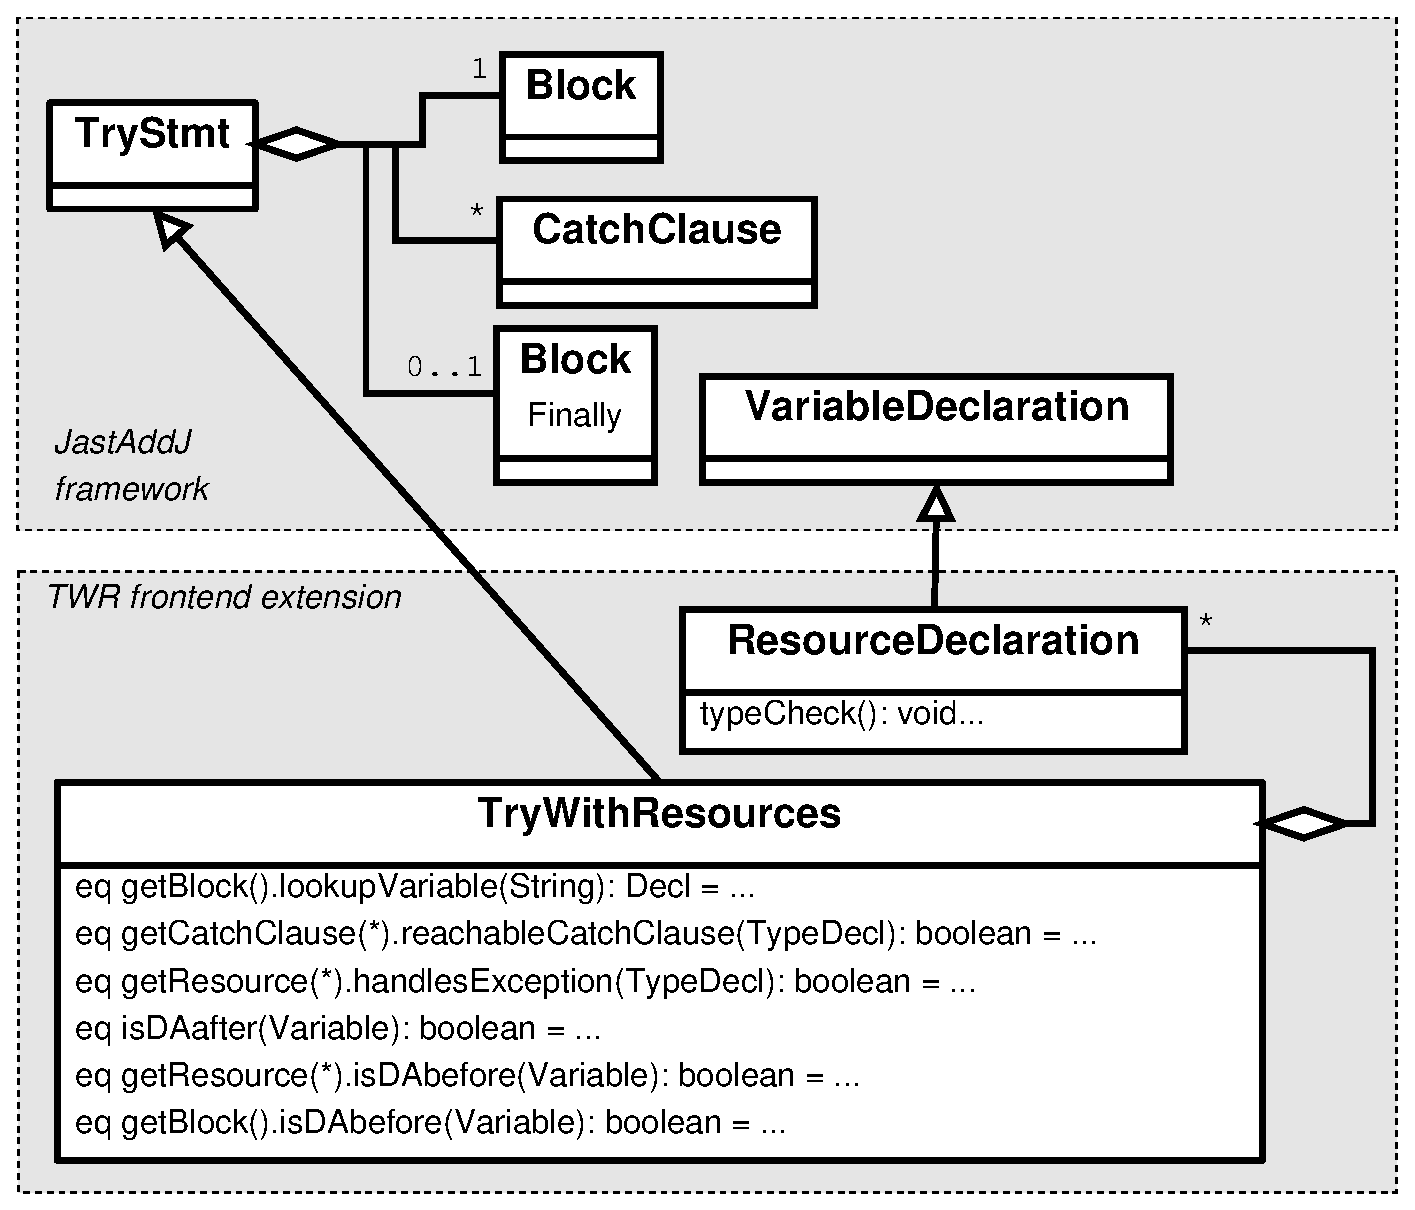
\includegraphics[width=\columnwidth]{figures/TWRextension.eps}
	\caption{\texttt{TryWithResources} and \texttt{ResourceDeclaration} are two new node types added to support TWR. The static semantics of TWR is adapted through equations and other declarations.}
	\label{TWRextension}
\end{figure}

\subsection{TWR code generation}

While the \verb'TryWithResources' node type conveniently describes the static semantics of the
TWR statement, implementing code generation was trickier.
The TWR statement does many things implicitly that need explicit code
generation support.  The Java bytecode does not have built-in support for
auto-closing resources, so all the steps needed for managing resources
correctly need to be generated into bytecode.

The approach we used in JastAddJ builds on the fact that any TWR statement can be transformed into a regular \texttt{try} statement with a series of basic TWR statements nested inside it, as described in the Java Language Specification \cite[p. 408]{jls7}. A \emph{basic TWR} statement has no catch clauses or finally clause--it has only resource declarations and a block. By transforming a TWR statement this way, the bytecode generation for the \texttt{try} statement can be reused, and the generation of the autoclosing support can be implemented in a simple way for the basic TWR nodes.

We implemented this approach by introducing the transformed version of the TWR statement as a \emph{non-terminal attribute} (NTA), i.e., an attribute whose value is a new AST subtree. The original TWR is used for static-semantic analysis, allowing any compile-time errors to be more closely related to the original source code. The code generation for a TWR is delegated to the transformed version of the statement, i.e., to the NTA. Figure~\ref{TWRbackend} outlines the extensions done in the Java~7 backend. Note that the NTA and the code generation method are added to the \texttt{TryWithResources} node type using \emph{inter-type declarations}. Inter-type declarations allow features of classes to be added in separate modules \cite{1997aspect}.

\begin{figure}
	\centering
	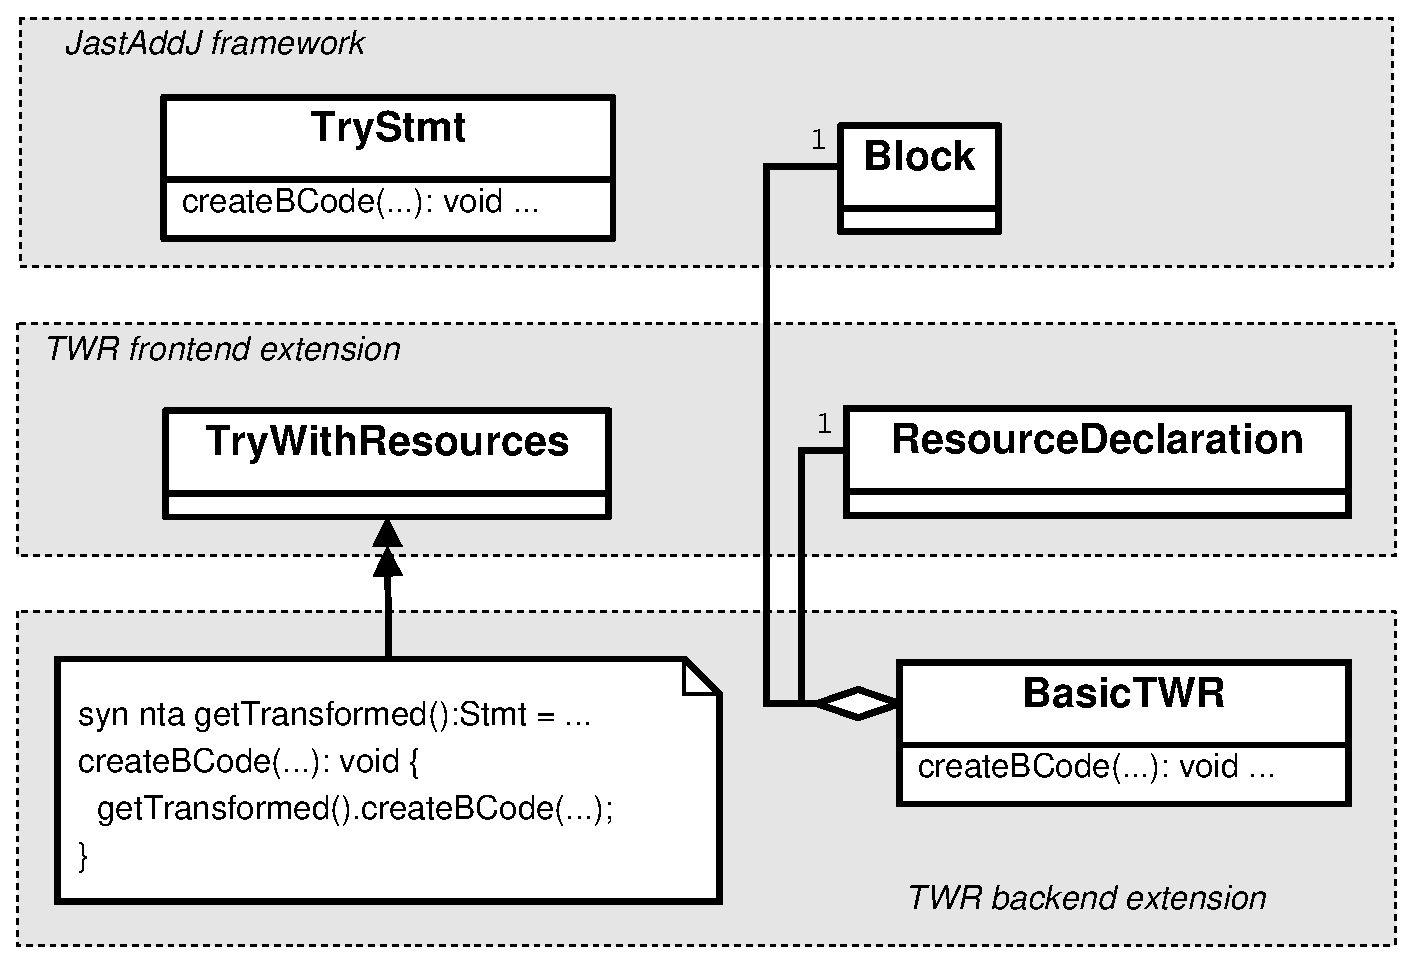
\includegraphics[width=\columnwidth]{figures/TWRextensionBackend.eps}
	\caption{To implement code generation for TWR, a \texttt{BasicTWR} node type is introduced, whose code generation handles autoclosure. The code generation method for the TWR statement delegates to the NTA \texttt{getTransformed}, which will be either a \texttt{TryStmt} or a \texttt{BasicTWR} statement. The double-arrowed relation indicates features added to an existing class using inter-type declarations.}
	\label{TWRbackend}
\end{figure}

The transformed version of a TWR may contain a new (simpler) TWR which in turn has an NTA containing its transformed version, so the transformation is carried out in several steps. Furthermore, we defined the \texttt{BasicTWR} to include only a single resource declaration, so if the original TWR contains several resource declarations, this will result in a transformed AST with several nested \texttt{BasicTWR} nodes. Figure~\ref{TWRexpansion} shows an example. A TWR (1) with catch clauses and/or a finally block is transformed to a regular \texttt{try} statement (2), including a new simpler TWR statement (3) with only resource declarations and a block. This simpler TWR statement is transformed into a \texttt{BasicTWR} (4) with one resource declaration, and any remaining resource declarations are included in a yet simpler TWR statement (5). This expansion terminates when the last resource declaration is handled by a \texttt{BasicTWR} (6).

%any TWR statement
%can be transformed into a set of nested \verb'try' statements \cite{jsr334}.  Using a
%transformed version of a TWR statement we can reuse the code generation for the
%\verb'try' statement to generate TWR bytecode.

%The transformed version of a TWR statement is introduced in the AST as an
%\emph{non-terminal attribute} (NTA), i.e., an attribute whose value is a new AST subtree. This way, both the original TWR statement, and its transformed counterpart will be part of the AST. The original TWR is used for static-semantic analysis, allowing any compile-time errors to be related to the original source code. The transformed statement is used for bytecode generation, allowing us to reuse the existing code generation for the \texttt{try} statement.

%non-terminal child of the TWR node. We chose to add it as a nonterminal because
%this allows the error messages referene TWR-specific
%semantics, e.g., type errors can report that a resource must be
%\verb'AutoCloseable', rather than just giving a generic type incompatibility
%message.

\begin{figure}
	\centering
	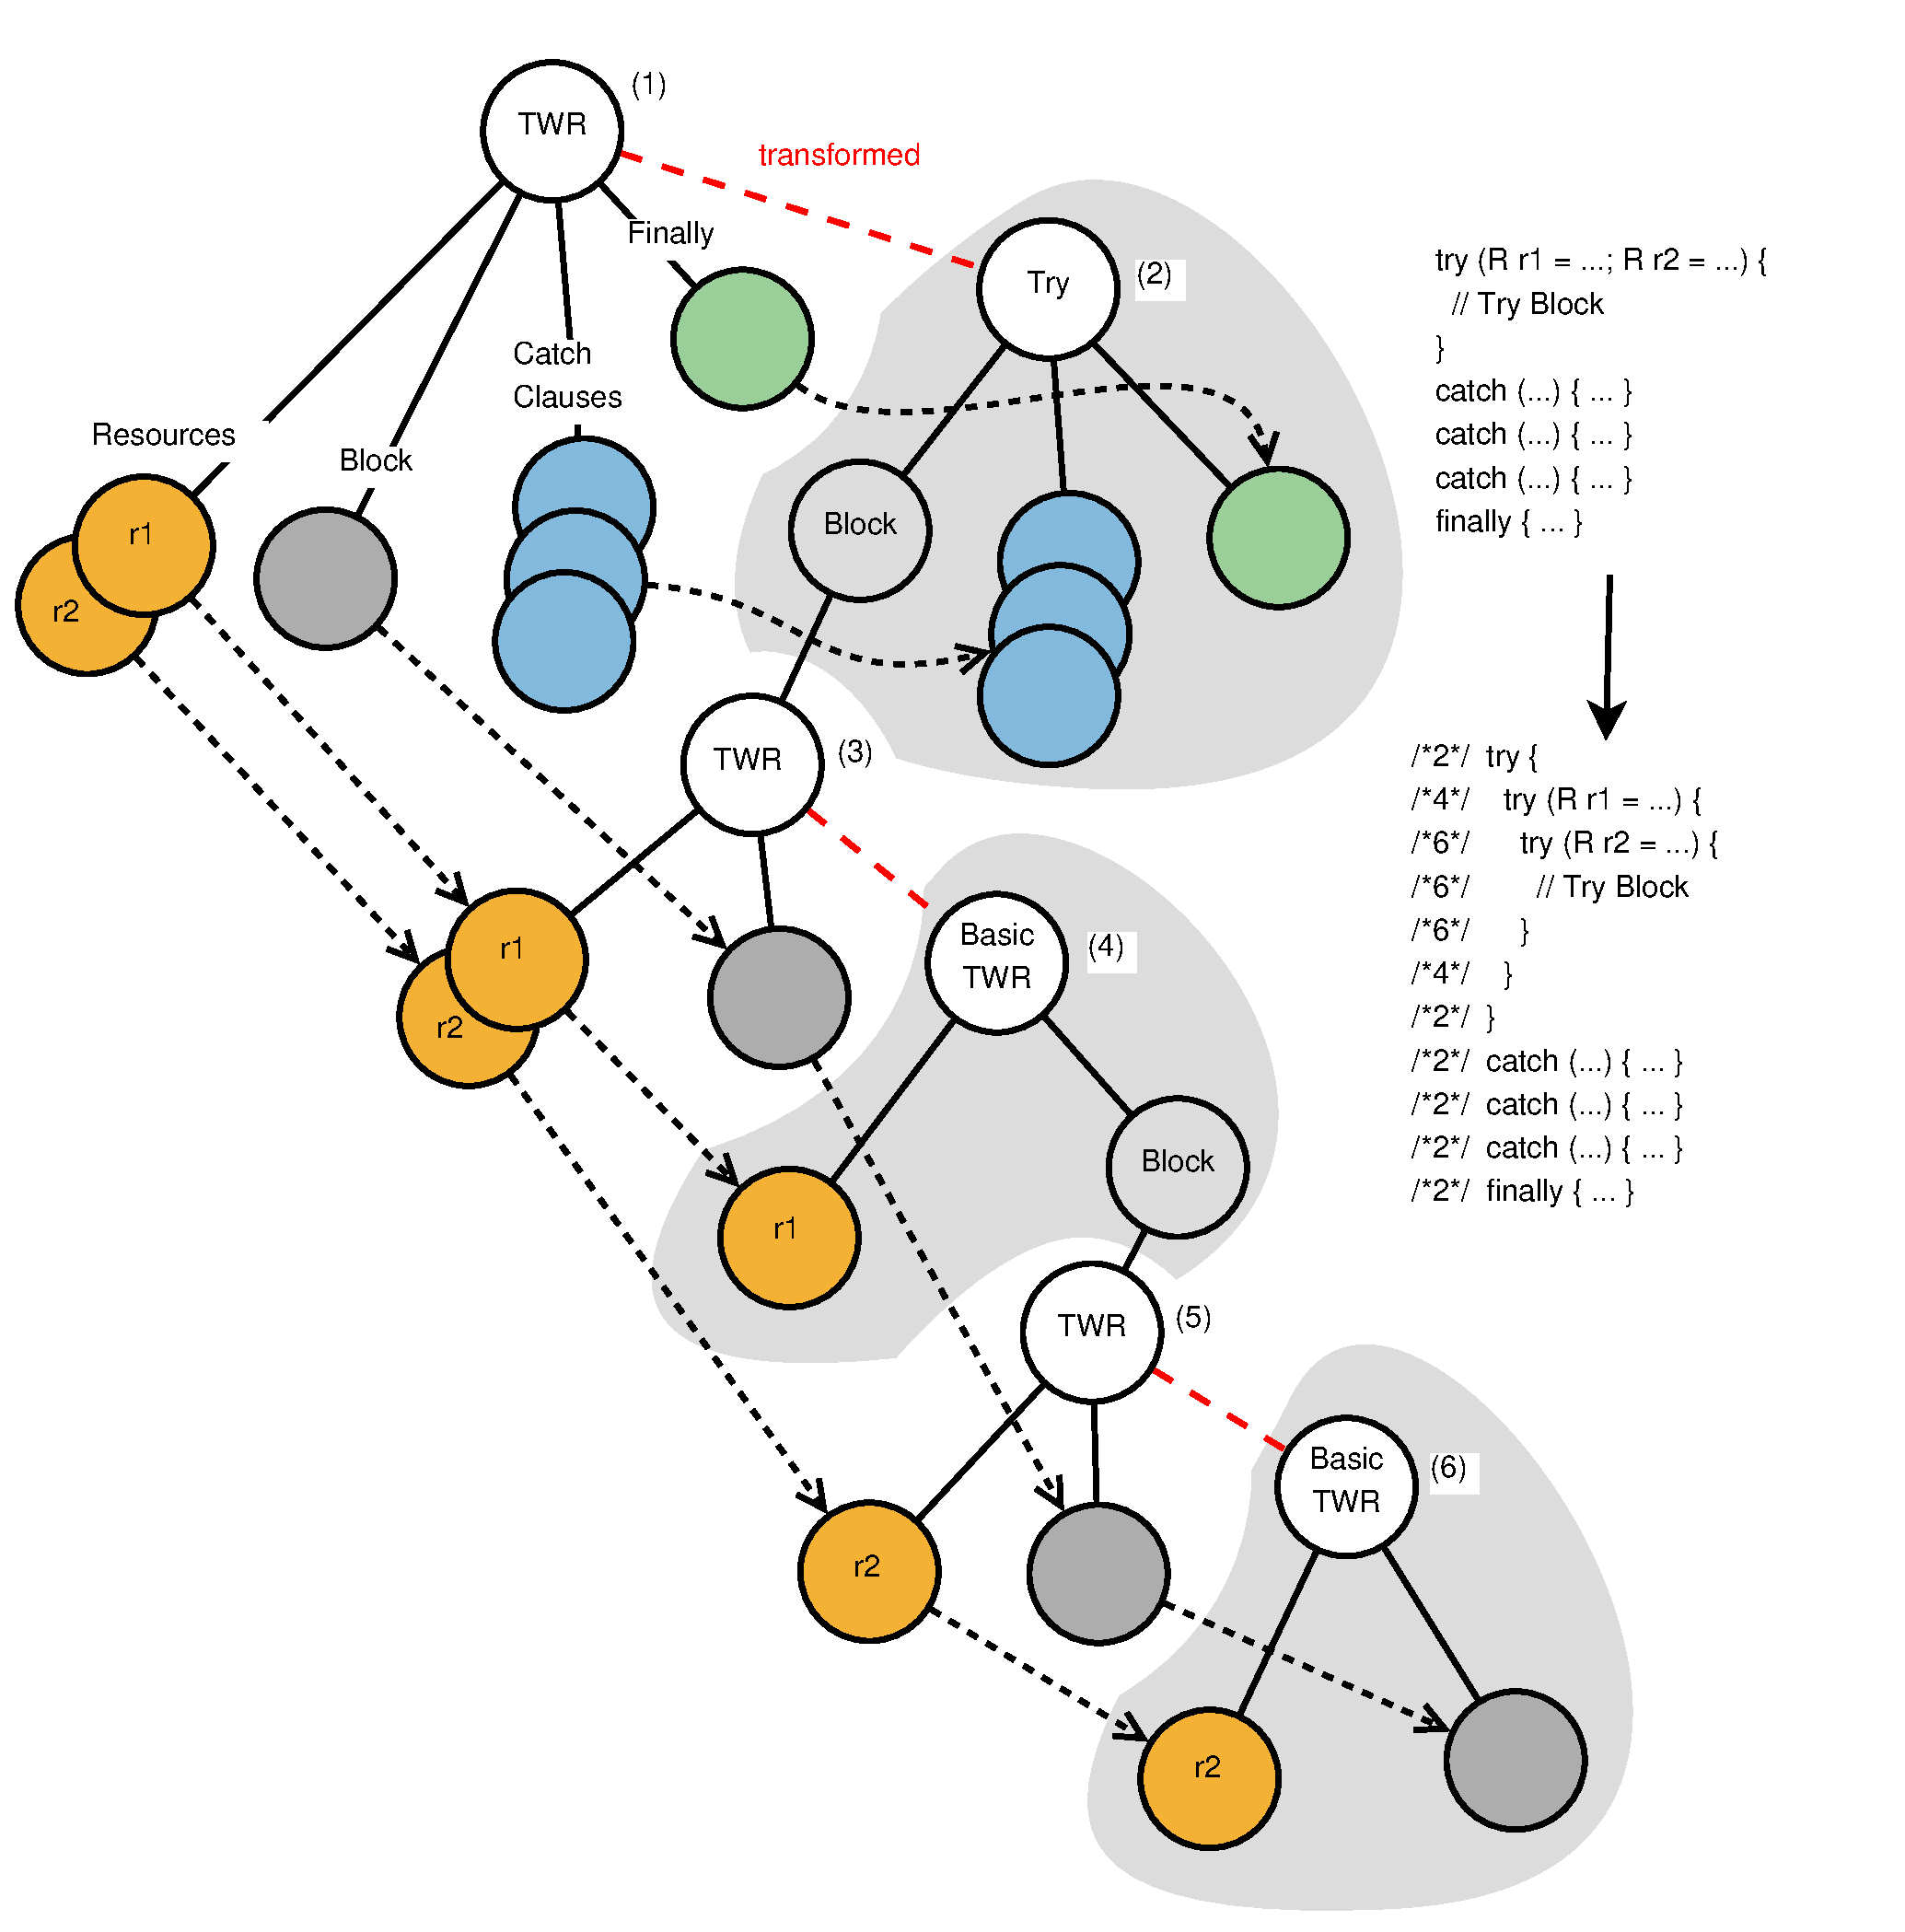
\includegraphics[width=\columnwidth]{figures/TWRtransform.eps}
	\caption{Example of stepwise transformation of a TWR statement using NTAs.
	An NTA \texttt{transformed} contains the new AST for each step.
	Lines without arrowheads indicate child-parent relationships, where the
	red dashed lines indicate NTA children. Dotted black arrows indicate AST
	nodes that are copied into an NTA. Grey shaded areas indicate transformed
	nodes to which code generation is delegated.}
	\label{TWRexpansion}
\end{figure}

%The Java Language Specification defines a special case of the TWR statement
%called \emph{basic} try-with-resources \cite[p. 408]{jls7}.
%A basic TWR statement has no catch clauses or finally clause. The specification
%also gives an equivalent form of the basic TWR statment expressed using
%a try-statement with (in the case of more than one resource declaration) a
%nested basic TWR statement.

%We use the basic TWR in JastAddJ to produce the transformed version of a
%TWR statement. First, the catch clauses and finally clause are moved to an
%enclosing \verb'try' statement. Then, the resulting basic TWR is transformed
%into a series of nested \verb'try' statements. Each transformation step can
%produce a new nested basic TWR, but with one fewer resource declarations than
%the previous basic TWR. This expansion terminates eventually with a simple
%\verb'try' statement.

\section{The Diamond Operator}
\label{Diamond}

In Java~7 the \emph{diamond operator} was added to reduce some of the
redundantly verbose nature of Java generics.

The diamond operator, \verb'<>', allows omission of type arguments for generic
class instance creations in some contexts (assignments, variable/field
initializers, method/constructor arguments). For example, instead of writing

\begin{lstlisting}
List<Integer> myList = new LinkedList<Integer>();
\end{lstlisting}

\noindent
Java~7 allows us to write the following shorter and more readable code:

\begin{lstlisting}
List<Integer> myList = new LinkedList<>();
\end{lstlisting}

%This is a small change, but it makes the code shorter and more readable.

\noindent
The compiler needs to infer omitted type parameters, i.e., \texttt{Integer} in
this case. To accomplish this, we added a new node type, \verb'DiamondAccess',
to represent diamond expressions such as \texttt{LinkedList<>} above.  It is
defined as a subtype of the existing type \verb'Access', allowing it to occur
in a class instance expression, see Figure~\ref{DiamondExtension}.

\begin{figure}
	\centering
	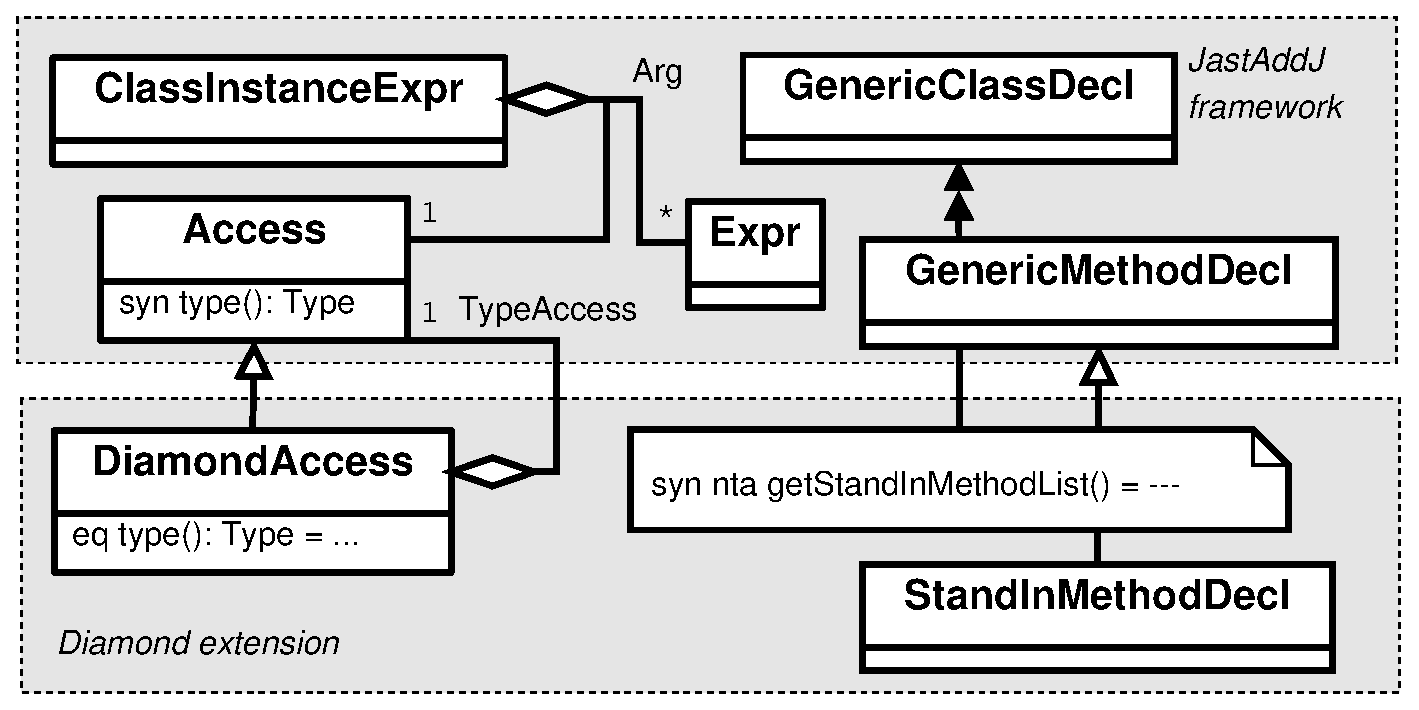
\includegraphics[width=\columnwidth]{figures/DiamondExtension.eps}
	\caption{To support the diamond operator, the JastAddJ frontend is extended with two new node types, \texttt{DiamondAccess} and \texttt{StandInMethodDecl}, and an NTA in the existing type \texttt{GenericClassDecl}.}
	\label{DiamondExtension}
\end{figure}

%When JastAddJ parses a type name followed by an empty
%type argument list it builds a \verb'DiamondAccess' node. The diamond operator
%is only legal if it is part of a class instance expression.

The parent \verb'ClassInstanceExpr' will query its \texttt{Access} child for
its \texttt{type} attribute.  The \texttt{DiamondAccess} node provides an
equation that computes the type attribute by performing type inference: first a
set of candidate constructors is computed, and then the most applicable
constructor and type argument set is found.

It turns out that this problem can be transformed into a similar problem of
inferring method type arguments for generic method invocations, a problem that
was solved already for Java~5. We could implement the diamond inference quite
easily, reusing the existing inference solution by creating a stand-in method
declaration for each candidate constructor.

Figures \ref{DiamondExtension} and \ref{fig:diamond} illustrate the extension.
To represent candidate constructors, a new type, \texttt{StandInMethodDecl} was
added, inheriting from the \texttt{GenericMethodDecl} type used by the existing
type inference algorithm. 

%The type inference for the diamond operator is performed by the
%\verb'DiamondAccess' node. The parent \verb'ClassInstanceExpr' will query it
%for it's type.  When JastAddJ infers type arguments for a diamond operator it
%first computes a set of candidate constructors, then it must find the most
%applicable constructor and type argument set. This problem can be transformed
%into the similar problem of inferring method type arguments for a generic
%method invocation. The inference of generic method type arguments was added to
%the Java language in Java~5 and was previously implemented in JastAddJ, so we
%decided to try to reuse this analysis for the diamond operator.
%
%In order to use the existing inference algorithm we construct a list
%of candidate methods.

A candidate method set is created using all accessible
constructors for the class to be instantiated. Let $C$ be the generic class to
be instantiated, with $T_{1 \ldots n}$ as its type parameters. For each
accessible constructor $K_i$ of $C$ we create a stand-in method $M_i$ with the
same parameter list as $K_i$ and return type $C<T_1, T_2, \cdots, T_n>$. The
stand-in methods $\{M_{1 \ldots m}\}$ are passed to the existing
inference algorithm which computes the most applicable method $M_j$ and
inferred type arguments. This gives us the most applicable constructor ($K_i$)
and the full type argument list for the instance creation. The candidate method
set is represented by a new NTA \verb'getStandInMethodList' added to the type
\verb'GenericClassDecl'.

%The stand-in methods are represented using \verb'MethodDecl' nodes. These are
%computed by the nonterminal attribute  

\begin{figure}
	\centering
	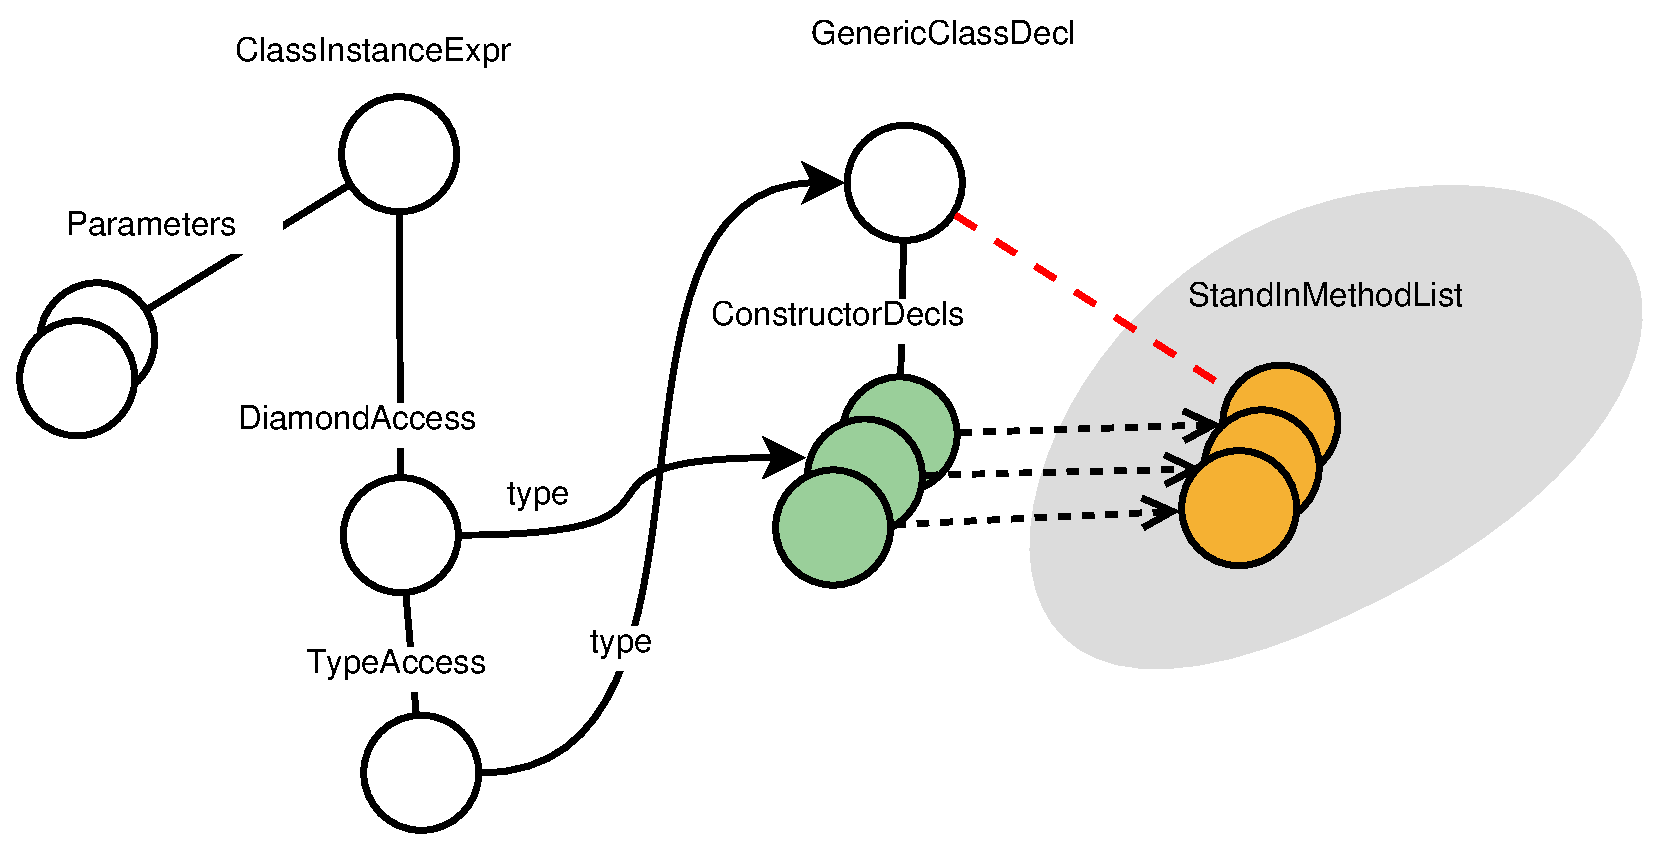
\includegraphics[width=\columnwidth]{figures/Diamond.eps}
	\caption{The Diamond type analysis reuses the Java~5 method type inference by computing stand-in methods using an NTA (the red dashed line). Solid arrows represent the \texttt{type} attributes. Dotted black arrows indicate construction of stand-in method declarations from constructor declarations.}
	\label{fig:diamond}
\end{figure}



\section{Evaluation}
\label{sec:evaluation}

In 2007, JastAddJ was compared to several other Java  compilers, including
Sun's \emph{javac} compiler \cite{jastaddj}. JastAddJ was then found to be less
than three times slower than javac, and with an implementation size of 66\% of
javac (counted in source lines of code). The execution speed of the generated
code was roughly the same for most programs.

Since 2007, both JastAddJ and javac have evolved, so it is interesting to do a
new comparison, and to include the new Java~7 implementations. We have compared
the OpenJDK Java~6 and Java~7 versions of JastAddJ and javac on a number of
different open source benchmark programs. We compare source code size,
compilation speed, memory consumption. We also tested the execution speed of
the generated bytecode, and found that it was almost the same for JastAddJ and
javac, with the JastAddJ-generated code being around 2\% slower on the average. 

The particular versions tested were
builds 7.1.1-49 for JastAddJ (jastaddj-6, jastaddj-7), OpenJDK 6 b24 for
javac-6, and OpenJDK 7 b146 for javac-7.

All tests were carried out on a quad core Intel Core i7-3820 CPU clocked at
3.60GHz with 64 GiB of memory, running Linux Mint with Linux kernel version
3.5.0-17-generic. All measurements were taken using the 64-bit Server editions
of the IcedTea6 1.12.5 (javac-6, jastaddj-6) and IcedTea 2.3.9 (javac-7,
jastaddj-7) runtime environments.  IcedTea is a compatible Java implementation
based directly on the freely available OpenJDK source code.

\subsection{Implementation size}

As an estimate of implementation effort, we have measured the total source code
sizes of JastAddJ and javac, excluding comments and whitespace, using the
tool SLOC-Count \cite{sloccount}. Figure~\ref{ImplementationSize} shows the
results. We see that JastAddJ is just slightly more than half the size of javac: 55\% for Java~6,
and 52\% for Java~7.

%\textbf{TODO:} JastAddJ-6 is now 26 kSLOC, but in the jastaddj article,
%JastAddJ-5 was 21 kSLOC. Why this big difference?? Are the measurements
%correct??

% Jag tror att siffrorna stämmer - jag har mätt om på gamla versioner av JastAddJ
% /Jesper

\begin{figure}[h]
\center
\small
\begin{tabular}{| c | c |}
\hline
\emph{Compiler} & \emph{kSLOC (\% of javac)}\\
\hline
javac OpenJDK 6 b24 & 47.4 (100\%)\\
JastAddJ 7.1.1-49 Java 6& 26.0 (55\%)\\
\hline
javac OpenJDK 7 b146 & 55.1 (100\%)\\
JastAddJ 7.1.1-49 Java 7 & 28.7 (52\%)\\
\hline
\end{tabular}
\caption{The source code size of the compilers, in thousands of source lines of code, and in percentage of javac.}
\label{ImplementationSize}
\end{figure}

\subsection{Compilation speed}

We have measured the mean time to compile a number of different benchmark
programs using Java~6 and 7 versions of javac and JastAddJ. We measured both
the compile time when the compilers are invoked in a fresh Java VM (see section
\ref{fresh-jvm}), as well as the steady-state compile time (section
\ref{steady-state}).

All time measurements were run with 2 GiB heap space, with JIT-compilation
enabled to allow each compiler to run at its optimal performance. The 2 GiB
heap space is well above the minimum required heap space for each benchmark
program (see figure \ref{fig:bm-mem}).

The benchmark programs we have used and their corresponding SLOC counts are
listed in the table in figure \ref{fig:bm-programs}.

\begin{figure}[h]
\centering
\small
\begin{tabular}{|l|l|r|l|}
  \multicolumn{1}{c}{\emph{Name}} &
  \multicolumn{1}{c}{\emph{Version}} &
  \multicolumn{1}{c}{\emph{kSLOC}} &
  \multicolumn{1}{c}{\emph{Description}} \\
  \hline
  %jdepend & 2.9.1 & 2.5 & Java dependency analyzer \\
  junit & 4.5 & 5.2 & Java unit testing framework \\
  jsilver & 1.0.1-SS & 30.1 & HTML template system \\
  %antlr & 2.7.2 & 34.6 & Aspect programming system \\
  clojure & 1.3.0-RC0 & 35.8 & Clojure compiler \\
  lucene & 3.0.1 & 45.3 & Text search engine \\
  javac & jdk7-b146 & 55.1 & OpenJDK 7 javac \\
  jython & 2.2alpha1 & 76.4 & A Python environment in Java \\
  jastaddj & R20111208 & 87.3 & JastAddJ (generated Java code)\\
  \hline
\end{tabular}
\caption{Benchmark programs}
\label{fig:bm-programs}
\end{figure}

\subsubsection{Fresh JVM compilation time}
\label{fresh-jvm}

For each benchmark-compiler pair the benchmark program was compiled 25 times --
each time in a new JVM instance.  The total time to run each invocation of the
compiler was measured (including JVM startup time).  The arithmetic mean of the
measured compile time is presented in figure \ref{fig:bm-time} (labeled without
the \verb'ss-' prefix).  Since JVM startup time was measured as part of the
total compile time we can expect a smaller relative difference in execution
time for the smaller benchmark programs (e.g. junit).

\begin{figure}
	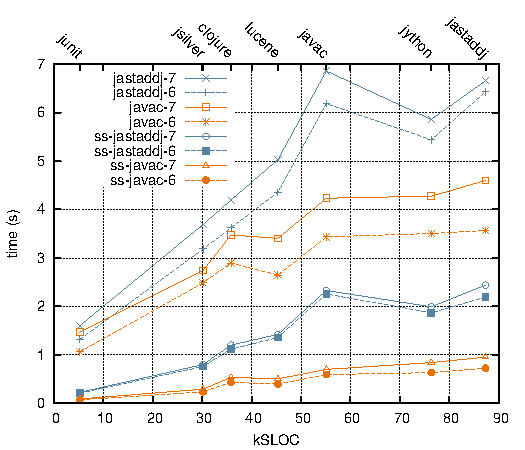
\includegraphics[width=\textwidth]{figures/bm-time}
	\caption{Compilation time. Includes times measured for fresh JVM
	invocations (top four curves) and steady-state execution (bottom four curves). Benchmarks are ordered from left
	to right by increasing SLOC count.}
	\label{fig:bm-time}
\end{figure}

\subsubsection{Steady-state compile time}
\label{steady-state}

We measured steady-state compile time using the method described in
\cite{georges2007statistically}.  A brief summary of the benchmarking
procedure:

\begin{itemize}
	
	\item For each benchmark-compiler pair we run 10 new JVM invocations.

	\item For each JVM invocation the benchmark program is compiled until the
		last 15 measured execution times have a coefficient of variance no
		greater than $0.05$.

	\item The mean of the last 15 compile times for the JVM invocation is
		calculated and stored.

\end{itemize}

The mean steady-state execution time of the 10 JVM invocations for each
benchmark-compiler pair is plotted in figure \ref{fig:bm-time} (labeled with
the \verb'ss-' prefix).

Using a Student's T distribution we calculated the 90\% confidence intervals
for each benchmark and found that they lie within 3\% of the mean execution
time (both for steady-state and fresh JVM).

Much of the time increase from Java~6 to Java~7 compilation is probably due
to the extra parsing time required to parse the larger Java~7 class library.

\subsection{Memory consumption}

We also compared the minimum required JVM heap space to run each
benchmark-compiler combination.  We found the minimum heap space by
doing a binary search from an initial 2048 MiB heap size to the lowest
heap size at which it was still possible to compile the benchmark program.
The minimum measured heap sizes are illustrated in figure \ref{fig:bm-mem}.

\begin{figure}
	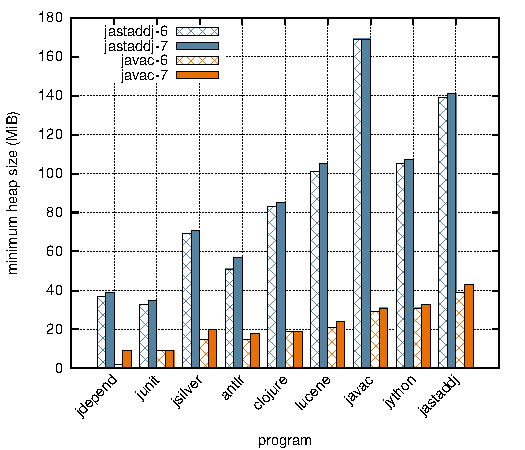
\includegraphics[width=\textwidth]{figures/bm-mem}
	\caption{Minimum heap space. Benchmarks ordered from left to right by
	increasing SLOC count.}
	\label{fig:bm-mem}
\end{figure}

\section{Related Work}
\label{sec:related-work}

%Related Work

OpenJDK is the reference implementation of the Java language, and is implemented in Java. It is
based on a traditional compiler pipeline with a series of phases that are called one after the
other. It is not specifically designed for language extension, and different language versions like
Java~6 and Java~7 are kept in different parallel repositories \cite{openjdk6}. Language extensions of OpenJDK need to copy and modify source files. For example, OpenJML is an implementation of JML (Java Modeling Language), and is built as a language extension to OpenJDK by modifying 41 of its 683 source files \cite{cok2011openjml}.

Polyglot \cite{nystrom2003polyglot} and AbleJ \cite{VanWyk2007AbleJ} are Java compiler frontends, built specifically to be extensible. Being frontends, they do scanning, parsing, and static semantic checking, but they do not generate bytecode.

Polyglot is implemented as a Java framework, and performs the frontend analysis as a series of
passes, most of which are implemented using a variant of the Visitor design pattern. The original
version supported Java~1.4, and recently, in 2012, support for Java~5 was released, implemented as a
modular extension of the Java~1.4 version \cite{polyglot-web}. So far, there is no support for Java~7 released.

AbleJ is implemented using the attribute grammar system Silver \cite{Wyk2010Silver}, and supports
most of Java~1.4. Modular extensions have been defined for supporting parts of Java~5 and SQL queries from within Java code \cite{VanWyk2007AbleJ}.

%Silver supports a mechanism called \emph{forwarding} \cite{vanwyk2002forwarding}, where attribute
%queries can be automatically forwarded to a nonterminal attribute (NTA), in essence giving the
%effect of a transformation. This mechanism is heavily used in AbleJ extensions to desugar new
%constructs to existing constructs in the base version of the language. For example, the Java~5
%enhanced-for statement creates a corresponding Java~1.4 statement as an NTA, and to which analyses can be automatically forwarded. The approach is slightly different in JastAddJ: In JastAddJ, the use of object-oriented mechanisms to inherit and override equations obviates much of the use for automatic forwarding: subtypes can be created that automatically reuse behavior from the supertype. We do not generally use NTAs for desugaring during analysis, as we want to be able to supply compile-time messages in terms of the original source code. However, as explained for the TWR construct, using NTAs for representing desugared constracts is very useful for code generation in JastAddJ. 

The Java~7 extensions of JastAddJ were implemented by Jesper {\"O}qvist as a master's thesis project, and a more detailed account of the implementation is available in the report~\cite{Oqvist2012MSc}.

%JaCo http://lampwww.epfl.ch/~zenger/jaco/ . Very old. Does not support even Java~5. Probably skip.

%Pierre-Etienne Moreau, Tom ?? Probably not.

%Eelco Visser. Java implementation in Stratego?? Looks like a front end only.  And for Java~5 only. Does not seem to address extensibility for Java itself at least. Perhaps skip.

%JKit (David Pearce) http://homepages.ecs.vuw.ac.nz/~djp/jkit/ . Latest release in Sept 2010. Very experimental I think. Probably no outside users. Probably does not work for any sizable programs.



\section{Conclusion}
\label{java7:sec:conclusions}

We have extended the JastAddJ Java~6 compiler to support Java~7. The extension
could be done modularly and concisely: the resulting source code for the
compiler is only 55 \% of that of OpenJDK javac for Java~6, and 52\% for Java
7. Thus, JastAddJ has grown less than javac since the Java~6 version.

We discussed some details of our implementation and how we could
extend the Java~6 implementation by adding new node types, equations and
attributes. In particular, the use of nonterminal attributes allowed us to
reuse code generation and type inferencing from Java~6 to implement the
Try-With-Resources statement and the Diamond operator.

We have measured the performance of our compiler to show that it is practical,
despite being a research compiler that is generated from a specification. When
run on a fresh JVM, our compiler runs within a factor of 1.6 compared to javac.
When run in steady state (like it would be run in an IDE), it runs within a
factor of 3.3 of javac for our benchmarks. Our compiler uses substantially
more memory than javac: 3.2 to 5.5 times as much memory as javac for our
benchmarks. However, with the memory capacity on today's computers, large
programs can still be compiled without problems.

%We have shown how a few Java~7 features were implemented in JastAddJ using
%nonterminal attributes. The use of nonterminal attributes allows expressing
%new language constructs using previously implemented ones and can both
%reduce code size and implementation complexity.

%\appendix
%\section{Appendix Title}
%
%This is the text of the appendix, if you need one.
%

% Acknowledgements
\section*{Acknowledgements}

This work was in part financed by the Swedish Research Council under
grant 621-2012-4727.

% We recommend abbrvnat bibliography style.

%\bibliographystyle{abbrvnat}

% The bibliography should be embedded for final submission.

{\raggedright
\printbibliography[segment=\therefsegment,heading=subbibliography]
}

}

\fi

\ifpaperII
\addtolength{\apa}{2cm}
\fancyhead[RE,LO]{Paper~II: Multitudes of Objects}
\chapter[Multitudes of Objects: First Implementation and Case Study for Java]{\texorpdfstring{%
Multitudes of Objects\\{\Large{}First Implementation and Case Study for Java}}{%
Concurrent Evaluation of Reference Attribute Grammars}}
\label{ch:multiplicities}
\paperRemark{\paperIIref}

%\affiliation{fernuni}{Lehrgebiet Programmiersysteme, Fernuniversität in Hagen, Germany}
%\affiliation{lu}{Lund University, Sweden}

{
% XeLaTeX stuff
%\setmonofont{Courier}

\makeatletter
\def\uwavered{\bgroup \markoverwith{\lower3.5\p@\hbox{\sixly \textcolor{red}{\char58}}}\ULon}
\font\sixly=lasy6 % does not re-load if already loaded, so no memory problem.
\makeatother

%\DeclareSortingScheme{customsort}{
%  \sort{\field{key}}
%}
%
%\AtEveryBibitem{\clearfield{url}}% remove doi urls

\makeatletter
\newenvironment{CenteredBox}{%
\begin{Sbox}}{%
\end{Sbox}\centerline{\parbox{\wd\@Sbox}{\TheSbox}}}%
\makeatother

\def\something{\ldots}

%\renewcommand{\ttdefault}{pcr}
\lstset{
  language=Java,%
  showstringspaces=false,
  %emph={abstract},%
  %emphstyle={\color{black}\bfseries\underbar},%
  morekeywords={any,option},%
  basicstyle=\ttfamily,
  %columns=flexible,%
  mathescape=true%
  %literate=
    %{*(}{\color{blue}}1
    %{)*}{\normalcolor}1
}

%\newcommand{\g}[1]{{\setlength{\fboxsep}{0pt}\colorbox{lightgray}{#1}}}
\newcommand{\g}[1]{\adjustbox{bgcolor=lightgray}{\strut{}#1}}
\newcommand{\f}[1]{\textbf{#1}}

\usetikzlibrary{matrix,shapes.multipart,trees,calc,arrows}

\renewcommand*{\sectionautorefname}{Section}
\renewcommand*{\subsectionautorefname}{Section}
\renewcommand*{\subsubsectionautorefname}{Section}

\section*{Abstract}

In object-oriented programs, the relationship of an object to many
objects is usually implemented using indirection through a collection. This
is in contrast to a relationship to one object, which is usually implemented
directly. However, using collections for relationships to many objects does
not only mean that accessing the related objects always requires accessing
the collection first, it also presents a lurking maintenance problem that
manifests itself when a relationship needs to be changed from to-one to
to-many or vice versa. Continuing our prior work on fixing this problem, we
show how we have extended the Java 7 programming language with
multiplicities, that is, with expressions that evaluate to a number of
objects \emph{not} wrapped in a container, and report on the experience
we have gathered using these multiplicities in a case study.

\begin{flushright}
  \emph{ein Vieles, welches kein Eines ist}\\
  (\emph{a multitude which is not a one})\\
--- inspired by Georg Cantor's conception of a set as ``jedes Viele, welches
sich als Eines denken l{\"a}{\ss}t'', i.e., any multitude which can be thought of as a
one
\end{flushright}

\section{Introduction}

\noindent Just like English grammar distinguishes singular and plural,
object-oriented programming languages distinguish one object and many
objects. However, unlike with English utterances, for which the syntactic
difference between the singular and the plural of a noun phrase is usually
small, the difference between program fragments dealing with one object and
dealing with many objects is often substantial. For instance, while the
English utterances ``I go to work'' and ``we go to work'' differ only
in the pronoun used, in an object-oriented program, the difference would be
that between \inline{i.goto(work)} and \inline{for (each : we) each.goto(work)},
which is cumbersome not only by comparison. The problem, here, is that in
object-oriented programming, the multitude denoted by \inline{we} is reified
as a one (usually a collection object), and this one has different
properties (responds to a different protocol) than the objects it comprises.
In particular, the object denoted by \inline{we} cannot go to work.

\begin{figure}
  \resizebox{\textwidth}{!}{%
  \begin{tikzpicture}[
      arrow/.style={
        ->,
        line width=1pt
      },
      divider/.style={
        draw=blue!40
      },
      heading/.style={
        fill=black!10
      }
    ]
    \node[draw] (c1) {\sffamily{Customer}};
    \node[draw,xshift=1.3cm,anchor=west] at(c1.east) (a1) {\sffamily{Account}};
    \draw[arrow] (c1.east) -> node[above,midway] {\footnotesize{\sffamily{account}}} node[below,near end] {\footnotesize{0..1}} (a1.west);

    \node[heading,anchor=south,yshift=5mm] (one) at($ (c1.north west) !.5! (a1.north east) $) {to-one relationship};

    \node[heading,anchor=east,xshift=-4mm] at(c1.west) {modelling};

    \node[anchor=west,draw,xshift=1cm] (c2) at(a1.east) {\sffamily{Customer}};
    \node[draw,xshift=1.3cm,anchor=west] at(c2.east) (a2) {\sffamily{Account}};
    \draw[arrow] (c2.east) -> node[above,midway] {\footnotesize{\sffamily{account}}} node[below,near end] {\footnotesize{0..*}} (a2.west);

    \node[heading,anchor=south,yshift=5mm] at($ (c2.north west) !.5! (a2.north east) $) {to-many relationship};

    \node[anchor=north,yshift=-1cm,draw, rectangle split, rectangle split parts=2] (c3) at(c1.south) {
      \nodepart{one}\sffamily{Customer}
      \nodepart{two}\sffamily{account}
    };
    \node[draw,xshift=1.3cm,anchor=west] (a3) at(c3.one east) {\sffamily{Account}};
    \draw[arrow] (c3.two east) -> node[below,near end] {\footnotesize{0..1}} (a3.west);

    \node[heading,anchor=east,xshift=-4mm] (impl) at(c3.west) {programming};

    \node[anchor=north west,xshift=1cm,draw, rectangle split, rectangle split parts=2] (c4) at(a3.north east) {
      \nodepart{one}\sffamily{Customer}
      \nodepart{two}\sffamily{accounts}
    };
    \node[draw,xshift=1.3cm,anchor=west] at(c4.one east) (ac4) {\sffamily{Collection}};
    \node[draw,yshift=-8mm] at(ac4.south) (a4) {\sffamily{Account}};

    \draw[arrow] (c4.two east) -> node[below,near end] {\footnotesize{0..1}} (ac4.west);
    \draw[arrow] (ac4) -> (a4);
    \node[xshift=-5pt,yshift=5pt] at (a4.north east) {\footnotesize{0..*}};

    \coordinate[xshift=-5mm] (vcenter) at(c2.west);
    \coordinate[yshift=5mm] (hcenter) at(c3.north);
    \coordinate (p1) at(one.north -| vcenter);
    \coordinate (p2) at(a4.south -| vcenter);
    \coordinate (p3) at(impl.west |- hcenter);
    \coordinate (p4) at(ac4.east |- hcenter);
    \draw[divider] (p1) -- (p2);
    \draw[divider] (p3) -- (p4);

  \end{tikzpicture}
  }%resizebox
  \caption{Relationships to one and to many objects in
object-oriented modelling and programming languages: differences}
  \label{figure1}
\end{figure}

Similar to the English language, relational and object-oriented modelling
languages make only a small distinction between singular and plural or, more
specifically, between one object being associated with one other, or any
number of other objects \cite{ref8, ref9, ref10, ref28, ref36}. In these languages,
\emph{multiplicity}, also known as \emph{cardinality}, constrains
the number of times an object, or entity, may occur in a relationship or
association. Hence, a change from singular to plural (or vice versa)
requires little more than a corresponding change in multiplicity, as the top
half of \autoref{figure1} suggests. By contrast, in object-oriented programming
languages multiplicities are commonly coded in the declared type of a
variable (which is the type of the related object if it is only one, or the
type of a sequence, stream, or collection object if there are more). Here, a
change of multiplicity may require a major redesign of the program, as the
bottom half of \autoref{figure1} suggests (several more untoward consequences of such
a change will be presented below).

In previous work \cite{ref37}, we advocated the introduction of
\emph{multiplicities} as annotations of expressions indicating whether
an expression is singular or plural, i.e., whether it is expected to
evaluate to at most one object, or to any number of objects~(not reified).
This is to grant the programmer a more uniform treatment of relationships to
one object and relationships to many objects in object-oriented programs. In
this paper, we present an implementation of our ideas as an extension of the
Java programming language using the JastAddJ extensible Java compiler \cite{ref13},
and report on a case study we have conducted.

The remainder of this paper is organized as follows. To motivate our work,
we present in \autoref{section2} the peculiarities we observe when implementing
multitudes of objects using collections. In \autoref{section3}, we briefly describe
how enhancing object-oriented programming with multiplicities can generally
alleviate the associated problems, with \autoref{section4} specializing our proposal
for Java. \autoref{section5} describes our implementation of multiplicities as an
extension of the JastAddJ compiler for Java 7. In \autoref{section6}, we present
qualitative and quantitative findings from a case study extending JUnit with
multiplicities. Notes on related and future work conclude.

\section[Using Collections for Representing Multitudes of Objects]{\texorpdfstring{%
\raggedright Using Collections for Representing Multitudes of Objects}{%
Using Collections for Representing Multitudes of Objects}}
\label{section2}

\noindent Undoubtedly, collections are among the most useful abstractions in
object-oriented programming: they not only liberate the programmer from
manually implementing multitudes of objects as (static) arrays or dynamic
data structures (such as linked lists or trees), they also offer a uniform
protocol for bulk processing of these object using internal iterators
(\inline{foreach}, \inline{select}, \inline{collect}, etc.). And yet, the use of
collections for representing many (rather than one) objects comes with a
number of peculiarities which make dealing with multitudes of objects very
different from dealing with single objects.

\subsection{Multiplicity Determines Type}
\label{section2.1}

\noindent In a program in which every customer can have only a single
account, we may see code like

\begin{lstlisting}
Account account;
account = new Account();
account.check();
\end{lstlisting}

\noindent If however a customer can have several accounts, adjustment of
just the declaration to reflect this leads to an ill-typed program (faulty
expressions underlined):

\begin{lstlisting}
Set<Account> accounts;
$\uwavered{\texttt{accounts = \textbf{new} Account();}}$
$\uwavered{\texttt{accounts.check();}}$
\end{lstlisting}

\noindent Both errors result from the fact that \inline{accounts} (with a
plural ``s'' appended to express that there can be more than one) now has
type \inline{Set<Account>}, reflecting the changed multiplicity. However, intuitively,
what is expressed by the ill-typed program is rather clear: initialize
\inline{accounts} to hold just one account, and then check all accounts (which
happens to be only one here). To translate this to standard Java, we would
have to write

\begin{lstlisting}
Set<Account> accounts = new HashSet<>();
accounts.add(new Account());
for (Account account : accounts) account.check();
\end{lstlisting}

\noindent which means quite a change to the original program.

\subsection{Multiplicity Determines Meaning of \texttt{null}}
\label{section2.2}

\noindent When a variable represents an optional relationship to one object,
the value \inline{null} usually means that there is no relationship (but may
also mean failure to initialize):

\begin{lstlisting}
if (account != null) print(account);
else print("no account");
\end{lstlisting}

\noindent For a relationship to many accounts, relating to no account is
usually represented using an empty collection:

\vbox{
\begin{lstlisting}
if (accounts != null)
  if (! accounts.isEmpty())
    for (Account account : accounts) account.print();
  else print("no account");
else throw new Error("accounts not initialized");
\end{lstlisting}
}

\noindent Here, the value \inline{null} means failure to
initialize. Note that having \inline{null} as an element of a collection makes
no sense if the collection is to represent a relationship.

\subsection{Multiplicity Determines Subtyping Conditions}
\label{section2.3}

\noindent If \inline{SavingsAccount} is a subtype of \inline{Account}, writing

\begin{lstlisting}
SavingsAccount saving = new SavingsAccount();
Account account = saving;
\end{lstlisting}

\noindent is type-correct. However, when we change to many accounts, the
analogue

\begin{lstlisting}
Set<SavingsAccount> savings = new HashSet<>();
Set<Account> accounts = savings;
\end{lstlisting}

\noindent is ill-typed. Instead, we would have to write something like

\begin{lstlisting}
Set<? extends Account> accounts = savings;
\end{lstlisting}

\noindent \cite{ref24} which does however preclude write access to the set through
the variable \inline{accounts}, greatly limiting its use (especially when
considering that the singular \inline{account} can be used freely).

\subsection{Multiplicity Determines Encapsulation Strategy}
\label{section2.4}

\noindent It is considered good practice in object-oriented programming that
the fields of an object are encapsulated and, if necessary, made accessible
for clients using setter and getter methods. For collection-valued fields,
however, this is different \cite{ref16}: they are to be updated using \inline{add...($\something$)} and
\inline{remove...($\something$)} methods offered by the encapsulating object (where the ellipses
are replaced by the field's name), and if the collection as a whole is
to be retrieved, the getter should return a copy or an immutable wrapper
\cite{ref16}. This is so because the collection is considered a representation
object which clients should not be able to manipulate directly and of which
they should possess no aliases \cite{ref25}. This brings us directly to the next
point.

\subsection{Multiplicity Determines Availability of Relationship Aliasing}
\label{section2.5}

\noindent While assigning an object to a variable with reference semantics
always means creating an alias for the object, the semantics differ when the
variables are uniformly viewed as implementing relationships to objects, as
the following example demonstrates:

\begin{lstlisting}
Account backup = account;
account = null;
if (mistaken) account = backup;
\end{lstlisting}

\noindent Here, \inline{backup} is an alias for the to-one relationship
implemented by \inline{account}. This is different for

\begin{lstlisting}
Collection<Account> backups = accounts;
accounts.clear();
if (mistaken) accounts = backups;
\end{lstlisting}

\noindent where \inline{backups} is an alias for the collection denoted, and
not for the to-many relationship that is logically established, by
\inline{accounts}. Surely, the problem can be solved by keeping a copy of the
collection as backup, but copying is not needed for the to-one case.

\subsection{Multiplicity Determines Call Semantics}
\label{section2.6}

\noindent Continuing the previous example, it may seem awkward that the
method

\begin{lstlisting}
void clear(Collection<Account> accounts) {
  accounts.clear();
}
\end{lstlisting}

\noindent performs as intended (i.e., sets the relationship represented by
an actual parameter to ``no accounts''), while the analogous method for
the to-one case

\begin{lstlisting}
void clear(Account account) {
  account = null;
}
\end{lstlisting}

\noindent has no effect on actual parameters. While this may look like a
newbie's mistake to the seasoned programmer, it is still indicative of
a conceptual chasm, which culminates in the fact that in Java, it is
impossible to implement

\begin{lstlisting}
void swap(Object o1, Object o2)
\end{lstlisting}

\noindent with the suggested semantics, while implementing

\begin{lstlisting}
void sort(ArrayList<Object> os)
\end{lstlisting}

\noindent is not a problem. Note that escaping to call-by-reference for
\inline{swap($\something$, $\something$)} does not bridge the chasm --- not having to do so for collections
is just another peculiarity of using them for representing multitudes of
objects.

\subsection{Multiplicity Determines Meaning of the \texttt{final} Modifier}
\label{section2.7}

\noindent When a variable is declared as \inline{final}, it means that its
value cannot be changed after its initialization. For a variable
representing a relationship to a single object this means that the owner of
the variable is stuck with the related object for its whole lifetime. For a
variable representing a relationship to many objects implemented using a
collection, \inline{final} means that the holder of the relationship is stuck
with the collection --- its elements, and thus the conceptually related
objects, may change freely:

\begin{lstlisting}
final Account forLife = new Account();
forLife = null; // compile error

final Set<Account> allForLife = Arrays.asSet(forLife);
allForLife.clear(); // no problem
\end{lstlisting}

\section{Programming with Multiplicities}
\label{section3}

\noindent The core idea of object-oriented programming with multiplicities
as put forward in \cite{ref37} is that expressions may evaluate directly to any
number, or \emph{a multitude}, of objects. This is in
contrast to standard object-oriented programming, in which every expression
evaluates to either one object or to \inline{null} and in which multitudes of
objects are reified using special container objects (collections, sequences,
iterators, etc.). Note that, since multitudes are not reified in our
approach, they are always flat, i.e., there is no multitude of multitudes
(though it is possible to create a multitude of collections).

% removed colon after "Terminological Note"
\paragraph{Terminological Note} We use ``multitude of objects'' to denote many objects;
the term is to be distinguished from ``collection of objects'' or
``set of objects'', which each denote an entity in its own right. Note that for
this reason it makes no sense to speak of ``the elements'' or ``the
members of a multitude'', or even of ``the objects of a multitude'' (since
the objects of the multitude \emph{are} the multitude) --- if we want
to refer to one of many, we say just that, or ``one object among
a multitude''.

\subsection{Dynamic and Static Multiplicity}
\label{section3.1}

\noindent With expressions evaluating to any number of objects, the
\emph{dynamic multiplicity} of an expression is defined as the number
of objects it evaluates to. In the general case, the dynamic multiplicity of
an expression can only be determined at runtime. Therefore, we complement
dynamic multiplicity with \emph{static multiplicity}, which can be
declared and inferred at compile-time. In the following, the term
multiplicity refers to static multiplicity unless stated otherwise.

While dynamic multiplicities are cardinals, we distinguish mainly two
(symbolic) static multiplicities, which we call \emph{option} and
\emph{any}. \emph{Option} stands for no or one ob\-ject, while
\emph{any} stands for any number of objects. Other static
multiplicities are also conceivable (in particular, multiplicity \emph{one}, for
precisely one, will be useful; see below); however, since our focus here is
on eliminating as much as possible the differences between relating to zero or one and to any number of objects, \emph{option} and \emph{any} suffice.

\subsection{Separation of Multiplicity and Type}
\label{section3.2}

\noindent As long as multitudes of objects are reified, the multiplicity of
an expression (i.e., whether it evaluates to one or many objects) is coded
in its type: for multiplicity \emph{any}, this type is a collection
type (commonly parameterized with the member type, i.e., the type of the
elements of the collection), whereas for multiplicity \emph{option},
the type is the type of the optional object (see \autoref{section2.1}). Object-oriented
programming with multiplicities as put forward in \cite{ref37} separates
multiplicity from type in the declaration of variables and methods: for
instance, it allows one to write

\begin{lstlisting}
any Account accounts;
\end{lstlisting}

\noindent instead of

\begin{lstlisting}
Collection<Account> accounts;
\end{lstlisting}

\noindent for declaring that \inline{accounts} can hold any number of
\inline{Account} objects (note that it cannot hold a collection!), whereas

\begin{lstlisting}
option Account account;
\end{lstlisting}

\noindent which differs only in the multiplicity, is roughly equivalent to

\begin{lstlisting}
Account account;
\end{lstlisting}

\noindent meaning that \inline{account} can hold either no or one account
(see \autoref{section3.4} for the important difference).  Note that using
multiplicities, both \inline{account} and \inline{accounts} have the same type
\inline{Account}; they differ only in their declared multiplicities.

\subsection{Assignment Compatibility}
\label{section3.3}

\noindent While the types of \inline{account} and \inline{accounts} are the same
and, therefore, do not oppose their mutual assignment compatibility, their
multiplicities differ --- since \emph{option} is subsumed
by \emph{any}, \inline{account} can be assigned to \inline{accounts}, and

\begin{lstlisting}
any Account accounts = new Account();
\end{lstlisting}

\noindent is a legal assignment (cf.~\autoref{section2.1}). An assignment from
\emph{any} to \emph{option} is illegal, however; here, a
multiplicity downcast (from \emph{any} to \emph{option}) as in

\begin{lstlisting}
account = (option) accounts;
\end{lstlisting}

\noindent is required, but may fail at runtime (namely when \inline{accounts}
holds more than one object).

For variables with multiplicity \emph{any}, assignment is
complemented with adding to (\inline{+=}) and subtracting from (\inline{-=})
a multitude of objects, where the right-hand side of the update operations
can have multiplicity \emph{any} or \emph{option}.

   \inline{null} remains assignment compatible with every reference type;
also, it is assignment compatible with both multiplicity \emph{option}
and \emph{any} (and means ``related to no object'' in both cases;
cf.~\autoref{section2.2}).

\subsection{Member Access}
\label{section3.4}

\noindent That \inline{account} and \inline{accounts} have the same type means
that they respond to the same protocol, i.e., that the same set of methods
can be invoked and the same set of fields can be accessed on them. For
instance, if class \inline{Account} defines a method \inline{check()}, both
\inline{account.check()} and \inline{accounts.check()} are well-typed; the
latter simply means that \inline{check()} is separately invoked on all objects
\inline{accounts} holds. If \inline{Account} declares an \emph{option} field \inline{bank},
\inline{accounts.bank} returns a multitude of bank objects, namely the
banks each account among the multitude of accounts held by \inline{accounts}
is related to. Note that if \inline{accounts} holds no object, or no account
referred to by \inline{accounts} has a bank associated with it,
\inline{accounts.bank} will evaluate to no object. Since \emph{option} is
subsumed by \emph{any}, \inline{account.bank} will also evaluate to no object
if \inline{account} does not hold an account; note in particular that no null
pointer exceptions can arise from dereferencing expressions whose
multiplicity is \emph{option} or \emph{any}.\footnote{For the relationship of the multiplicity \emph{option}
with the type \inline{Option} of some functional programming languages
(including Scala), see the related work in \autoref{section7}}

\subsection{Aliasing}
\label{section3.5}

\noindent In object-oriented programming with multiplicities, multitudes of
objects are not reified, so multitudes cannot be aliased. This retires the
problems noted in Sections~\ref{section2.3}--\ref{section2.6}. In particular,

\begin{lstlisting}
any SavingsAccount savings;
any Account accounts = savings;
\end{lstlisting}

\noindent does not cause a covariance problem, since the assignment does not
create an alias for a container, but instead assigns \inline{accounts} the
same multitude of objects that \inline{savings} refers to (by copying pointers
just like in the \emph{option} case). It follows that

\begin{lstlisting}
accounts += new Account();
\end{lstlisting}

\noindent does not also add an account to \inline{savings} (cf.~\autoref{section2.3}).
Likewise, returning \inline{accounts} as in

\begin{lstlisting}
any Account getAccounts() { return accounts; }
\end{lstlisting}

\noindent does not expose representation to clients (there is no
representation object representing the multitude held by \inline{accounts})
and, in particular,

\begin{lstlisting}
any Account temp = getAccounts();
temp += new Account();
\end{lstlisting}

\noindent does not update the field \inline{accounts} returned by the getter
(\autoref{section2.4}). Similarly, after the assignment

\begin{lstlisting}
any Account backups = accounts;
\end{lstlisting}

\noindent (\autoref{section2.5}), clearing \inline{accounts} (by assigning it \inline{null};
cf.~\autoref{section3.3}) does not also clear \inline{backups}, which is therefore still
available for restoration. Also, passing a variable into the method
\inline{clear($\something$)} of \autoref{section2.6}, now defined as

\vbox{
\begin{lstlisting}
void clear(any Account accounts) {
  accounts = null;
}
\end{lstlisting}
}

\noindent does not affect the number of objects that this variable holds,
thereby unifying the behaviour for one and many objects. Lastly, the fact
that multitudes of objects are not reified unifies the meaning of the
\inline{final} modifier (\autoref{section2.7}), which now pertains to variables holding
single object and multitudes of objects alike.

\subsection{When to and When Not to Use Multiplicities}
\label{section3.6}

Our motivation of introducing multiplicities to object-oriented programming
is to allow the programmer

\begin{itemize}
  \item the implementation of relationships (or, more precisely, directed
    associations \cite{ref28}) to many objects in a more direct way, and further
  \item the implementation of relationships to one and to many objects in as
    much the same way as possible.
\end{itemize}

\noindent This raises the question of what is a relationship, or when
multiplicities are to be used.

Experience teaches that programmers will use a construct wherever they
deem its use advantageous, so we attempt no dogmatism here. We still make
one exception, though: value types, like \inline{int}, \inline{float},
\inline{boolean}~(including their wrapper types), or \inline{String} (whose
instances are usually immutable) cannot be the target of a relationship
(note that they cannot act as entity types in the entity-relationship model
\cite{ref8}) and hence cannot be used in combination with \emph{option} or
\emph{any} multiplicity annotations. While there are conceptual
justifications for this (e.g., people do not relate to their age, an integer
value), the main technical reason is that this saves us from defining
special semantics for operations on value types (such as \inline{+}) for operands
with \emph{option} or \emph{any} multiplicity (which both include
``no object'' as a possible value), and also from introducing a ternary logic
for handling the case that a boolean expression used in a conditional
evaluates to no object. For instance, for a variable declared as
\inline{option boolean error}, it is unclear what \inline{if (error) ...} means
if \inline{error} has dynamic multiplicity 0. For the same reason, we must
exclude that value-typed members are accessed via receiver expressions with
\emph{option} or \emph{any} multiplicity, since this can likewise
result in dynamic multiplicity 0 (namely when the receiver evaluates to
``no object'').

\section{Multiplicities for Java}
\label{section4}

\noindent While the idea of object-oriented programming with multiplicities
as presented in the previous section is language-independent, its adoption
in any concrete language invariably requires an individualized integration
with existing language constructs. In the following, we present our
extension of Java 7 with multiplicities, whose design was driven by our
objective to allow a smooth transition between Java programming without and
Java programming with multiplicities. \autoref{figure2} has the extended syntax;
\autoref{figure3} shows some sample code using it.

\begin{figure}[h]
  \begin{CenteredBox}
\begin{lstlisting}[basicstyle=\ttfamily\small]
Modifier ::= ...
 | MultiplicityAnnotation;

MultiplicityAnnotation ::=
   "@any" "(" ReferenceType ")"
 | "@any"
 | "@option"
 | "@bare";

Primary ::=
 | "[[" UnaryExpressionNotPlusMinus "]]"
 | "|[" UnaryExpressionNotPlusMinus "]|";

CastExpression ::= ...
 | MultiplicityCastExpr;

MultiplicityCastExpr ::=
   "(" MultiplicityAnnotation ")" UnaryExpression
 | "(" MultiplicityAnnotation TypeName ")"
   UnaryExpression;
\end{lstlisting}
  \end{CenteredBox}
\caption{Extension of concrete syntax.}
\label{figure2}
\end{figure}

\begin{lrbox}{\lstboxleft}
\begin{lstlisting}[basicstyle=\ttfamily\footnotesize]
class Subject implements Observable {
  $\g{Set<}$Observer$\g{>}$ obs $\g{= new HashSet<>()}$;

  public void addObserver(Observer o) {
    $\g{if (o == null)}$
      $\g{throw new NullPointerException();}$
    obs$\g{.add(}$o$\g{)}$;
  }

  public void deleteObserver(Observer o) {
    obs.$\g{remove(}$o$\g{)}$;
  }

  public void notifyObservers(Object arg) {
    $\g{for (Observer o :}$ obs$\g{)}$
      $\g{o}$.update(this, arg);
  }

  public void deleteObservers() {
    obs$\g{.clear()}$;
  }

  public int countObservers() {
    return obs$\g{.size()}$;
  }
}
\end{lstlisting}%
\end{lrbox}

\begin{lrbox}{\lstboxright}
\begin{lstlisting}[basicstyle=\ttfamily\footnotesize]
class Subject implements Observable {
  $\g{@any(}$HashSet$\g{)}$ Observer obs;

  public void addObserver($\g{@option}$ Observer o) {


    obs $\g{+=}$ o;
  }

  public void deleteObserver($\g{@option}$ Observer o) {
    obs $\g{-=}$ o;
  }

  public void notifyObservers(Object arg) {

    obs.update(this, arg);
  }

  public void deleteObservers() {
    obs $\g{= null}$;
  }

  public int countObservers() {
    return $\g{|[}$obs$\g{]|}$;
  }
}
\end{lstlisting}%
\end{lrbox}

\begin{figure}[b!]
\begin{CenteredBox}
  \begin{tabular}{cc}
    original (without using multiplicities) & using multiplicities \\
    \hline
    \scalebox{0.8}{\usebox{\lstboxleft}}&%
    \scalebox{0.8}{\usebox{\lstboxright}}\\
  \end{tabular}
\end{CenteredBox}
  \caption{Example of implementing class \inline{Subject} of the Observer
    Pattern, with and without using multiplicities (differences highlighted)}
  \label{figure3}
\end{figure}

\subsection{Multiplicity Annotations}
\label{section4.1}

\noindent For compatibility with existing Java code, we implemented four
static multiplicities:

\begin{itemize}
  \item \emph{none}, the multiplicity of \inline{null} (representing no object);
  \item \emph{bare}, the default multiplicity (and, in particular, the
    multiplicity of all standard, or legacy, declarations);
  \item \emph{option}, the multiplicity of entities and expressions
    representing relationships to no or to one object; and
  \item \emph{any}, the multiplicity of entities and expressions representing
    relationships to any number of objects.
\end{itemize}

\noindent Multiplicities determine assignment compatibility according to the
order

\begin{equation*}
  none < bare < option < any
\end{equation*}

\noindent i.e., every multiplicity is assignment compatible with itself and
all greater ones.

\paragraph{Hidden Collections} To give the programmer control over the nature of
multitudes, and also for interfacing with legacy Java code that uses
collections (see below), \emph{any} multiplicities may be parameterized
with a collection type \emph{C} whose definition has a single type
parameter (e.g., \inline{List<E>}). This type will be used to instantiate a
\emph{hidden collection} holding the multitude of objects. To
acknowledge the widespread use of abstract collection types in Java
programs, \emph{C} may be an abstract class or an interface.

\paragraph{Syntactic Integration} The multiplicity \emph{none} does not occur in
program texts; the other multiplicities appear as annotations \inline{@bare},
\inline{@option}, and \inline{@any}, respectively (see~\autoref{figure2}). Since
\emph{bare} is the default multiplicity, it occurs only in multiplicity
downcasts from \emph{option} or \emph{any} to \emph{bare}
(see below).

\subsection{Declarations}
\label{section4.2}

\noindent The multiplicity annotations \inline{@option} and \inline{@any} may
appear (in the position of modifiers; cf. \autoref{figure2}) in all declarations of
reference-typed entities, except where the type is a wrapper type (such as
\inline{Boolean}) or \inline{String} (see \autoref{section3.6} for the reasons). If an
entity is annotated with \inline{@any(C)} and \inline{C} is a concrete
collection class, the compiler uses \inline{C} as the class of the hidden
collection that holds the multitude of objects the annotated entity denotes;
if \inline{C} is abstract or not provided, the compiler automatically picks a
suitable concrete class (note that the single type parameter of \inline{C} is
instantiated with the type of the declaration). Thus, multitudes of objects
\emph{are} implemented using collections; however, this implementation
is strictly under the hood and, in particular, these collections cannot be
accessed from the program as objects (they cannot be aliased). Entities
annotated with \inline{@option} are not implemented using collections;
however, the compiler gives their value \inline{null} a special meaning (see
below).

\paragraph{Final Declarations} A declaration \inline{final @option T v} means that,
after its initialization, the value of \inline{v} cannot change (i.e.,
\inline{v} always refers to the same object). That \inline{v} is not assigned
new values after initialization is ensured (by the compiler) as usual. A
declaration \inline{final @any T v} likewise means that \inline{v} cannot be
updated after its initialization (i.e., it always refers to the same
objects), where updating includes assignment (\inline{=}), adding objects (\inline{+=}), and
removing objects (\inline{-=}); this is ensured by the very same means. Hence,
no immutable collections are required to express the immutability of a
multitude.

\subsection{Interfacing with Collections: Wrapping and Unwrapping}
\label{section4.3}

\noindent To interface multiplicity \emph{any} with code that uses
(bare) collections for representing multitudes of objects, we must be able
to wrap a multitude in a collection object, and to unwrap it from a
collection object. We use double square brackets (``\inline{[[$\something$]]}'') for both purposes
(see \autoref{figure2}). If the argument expression has static multiplicity
\emph{any(C)}, the result is a (fresh) collection of type
\emph{C} holding the objects the expression evaluates to; if it has
multiplicity \emph{option}, the result is a new instance of class
\inline{ArrayList} which either holds the object the expression evaluates to,
or is empty if it evaluates to \inline{null}. We call this
\emph{wrapping}. If the argument expression has static multiplicity
\emph{bare} and is a collection, the result is the multitude of objects
that the collection holds (which is internally represented using a fresh
collection of the same type). We call this \emph{unwrapping}.
Unwrapping is particularly useful for initializing final variables with
multiplicity \emph{any}:

\begin{lstlisting}
final @any Account accounts =
  [[Arrays.asList(new Account(), new Account())]];
\end{lstlisting}

\noindent The expression \inline{[[null]]} is not allowed.

\subsection{Number of Objects}
\label{section4.4}

\noindent The dynamic multiplicity, or the number of objects an expression
evaluates to, is computed using ``\inline{|[$\something$]|}'' (see \autoref{figure2}). In case the argument
expression has multiplicity \emph{any}, it returns the size of the
underlying collection; if the expression has multiplicity
\emph{option}, it returns 0 if it evaluates to \inline{null}, and 1 else.

\subsection{Casts}
\label{section4.5}

As for types, multiplicity upcasts (e.g., from \emph{option} to
\emph{any}) are always safe and therefore may remain implicit.
Multiplicity downcasts from \emph{any} to \emph{option} or
\emph{bare}, however, may fail, namely when the \emph{any}
expression being cast evaluates to more than one object. Therefore, the
compiler inserts a runtime multiplicity check for all such casts which, upon
failure, throws a multiplicity cast exception. Casts from \emph{option}
to \emph{bare} are also always safe; since unlike for
\emph{option} receivers, accessing members on \emph{bare}
receivers can lead to null pointer exceptions, we will require explicit
downcasts from \emph{option} to \emph{bare} (see below for
examples of where this is needed).

\subsection{Expressions}
\label{section4.6}

\noindent With new syntax given meaning as above, we now turn to the impact
multiplicities have on standard Java expressions.

\paragraph{Update} Assignment (\inline{=}) makes the variable on the left-hand side refer to
the objects the right-hand side refers to. Given the arbitrariness of the
definition of ``identity of multitudes of objects'' for multiplicity
\emph{any} (see below), we defined assignment pragmatically: the hidden
collection holding the multitude of the left-hand side is first emptied
(cleared), and then all objects of the hidden collection representing the
right-hand side are copied into it using its \inline{addAll($\something$)} method. If the
right-hand side has multiplicity \emph{option}, its object (if any) is
added to the collection using \inline{add($\something$)}. If the left-hand side has
multiplicity \emph{option}, the object that the right-hand side
evaluates to is assigned to it.

Adding (\inline{+=}) is only allowed for left-hand sides with
\emph{any} multiplicity and adds the object(s) of the right-hand side
(if any) to it, again using \inline{add($\something$)} or \inline{addAll($\something$)}. Removing
(\inline{-=}) works accordingly, using the corresponding remove methods. Note
that the programmer can override the meaning of \inline{+=} and \inline{-=} by
supplying her own collection implementations to the \emph{any}
annotations in the declarations.

\paragraph{Member Access} Accessing a member \inline{m} on a receiver \inline{r} with
multiplicity \emph{any} unfolds to accessing \inline{m} on every object
among the multitude \inline{r} evaluates to, in the order provided by the
iterator of the hidden collection holding the multitude. If \inline{m} is a
field or a non-void method, \inline{r.m} evaluates to a multitude of objects,
independently of whether \inline{m} has multiplicity \emph{option} or
\emph{any} (recall that multiplicities are always flat). As argued in
\autoref{section3.6}, \inline{m} must not be \emph{bare}; if it is, the receiver
must be cast to \emph{bare} first (cf.~\autoref{section4.5} and \ref{section6.2.2}).

Since \emph{option} is subsumed by \emph{any}, accessing
\inline{m} on \inline{r} having multiplicity \emph{option} behaves exactly
as if \inline{r} had static multiplicity \emph{any} and dynamic
multiplicity 0 or 1. In particular, if \inline{r} is \inline{null}, evaluating
\inline{r.m} does not raise a null pointer exception --- it simply evaluates
to \inline{null} (for ``no object''). However, deviating from receiver
multiplicity \emph{any}, \inline{r.m} has multiplicity
\emph{option} for \emph{option} members (see \autoref{table1}).

\begin{wraptable}[9]{r}{6cm}
  \begin{tabular*}{6cm}{ l|@{\extracolsep{\fill}}ccc}
  \hline
  \diaghead{\emph{option}}{r}{m} & \emph{bare} & \emph{option} & \emph{any} \\
  \hline
  \emph{bare} & \emph{bare} & \emph{option} & \emph{any} \\
  \emph{option} & N/A & \emph{option} & \emph{any} \\
  \emph{any} & N/A & \emph{any} & \emph{any} \\
  \end{tabular*}
  \caption{Multiplicity of member access expressions \texttt{r.m}}
  \label{table1}
\end{wraptable}

If \inline{m} is a method, parameter passing works according to the rules of
assignment (see under ``Update'' above). In particular, the formal parameters
do not receive aliases to the hidden collections holding the objects of
formal parameters having multiplicity \emph{any}. Similarly, \inline{m}
does not return aliases to the hidden collection representing the returned
expression. Note that, with respect to multiplicity, overriding methods must
be contravariant in the formal parameter multiplicities (i.e.,
\emph{option} can be overridden with \emph{any} etc.) and
covariant in the return multiplicities (i.e., \emph{any} can be
overridden with \emph{option} etc.). \autoref{figure4} has an example of a
covariantly overridden method (\inline{getLeaves()}).

\begin{lrbox}{\lstboxleft}
\begin{lstlisting}[basicstyle=\ttfamily\footnotesize]
abstract class Composite {
  abstract $\g{List<}$Leaf$\g{>}$ getLeaves();
}

class Component extends Composite {
  $\g{List<}$Composite$\g{>}$ children$\g{ = new ArrayList<>()}$;
  $\g{List<}$Leaf$\g{>}$ getLeaves() {
    $\g{List<Leaf leaves = new ArrayList<>();}$
    $\g{for (Composite child : children)}$
      $\g{leaves.addAll(child.getLeaves());}$
    return $\g{leaves}$;
  }
}

class Leaf extends Composite {
  $\g{List<}$Leaf$\g{>}$ getLeaves() {
    return $\g{Arrays.asList(}$this$\g{)}$;
  }
}
\end{lstlisting}%
\end{lrbox}
\begin{lrbox}{\lstboxright}
\begin{lstlisting}[basicstyle=\ttfamily\footnotesize]
abstract class Composite {
  abstract $\g{@any}$ Leaf getLeaves();
}

class Component extends Composite {
  $\g{@any}$ Composite children;
  $\g{@any}$ Leaf getLeaves() {



    return $\g{children.getLeaves()}$;
  }
}

class Leaf extends Composite {
  $\g{@option}$ Leaf getLeaves() {
    return this;
  }
}
\end{lstlisting}
\end{lrbox}

\begin{figure}[b!]
\begin{CenteredBox}
  \begin{tabular}{ll}
  original (without using multiplicities) & using multiplicities \\
  \hline
  \scalebox{0.9}{\usebox{\lstboxleft}}&%
  \scalebox{0.9}{\usebox{\lstboxright}}\\
  \end{tabular}
\end{CenteredBox}
  \caption{Example of implementing a composite structure with and without using
  multiplicities (differences highlighted)}
  \label{figure4}
\end{figure}

\paragraph{Test for Identity} Strictly speaking, a test for identity (``\inline{==}'') does
not make sense for multitudes of objects: if multitudes are not reified, how
can they be identical? On the other hand, if the dynamic multiplicities of
the left-hand side and the right-hand side of such a test are 0 or 1, there
seems little choice in defining the meaning of \inline{==}\,: it is true if and only if
either both evaluate to the same object, or both evaluate to \inline{null}.
For greater numbers of objects, it would seem reasonable to require that
both sides have the same dynamic multiplicities; yet, this means that even
immediately after an assignment of an expression having multiplicity
\inline{@any(List)} to a variable having multiplicity \inline{@any(Set)},
identity may not be given (due to the dropping of duplicate objects). In
practice, what it means for two multitudes to be identical (or only equal)
is at least as variable as what it means for two collections to be equal, so
that eventually, the programmer must be given control over this question (by
letting her implement her own tests). Therefore, we made an arbitrary choice
for \inline{==} and implemented it as each object from each multitude occurring
exactly the same number of times in both multitudes. Note that for a test of
equality using the \inline{equals($\something$)} methods provided for collections, the
multitudes must be wrapped first (see \autoref{section4.3}).

\paragraph{Iteration over Multitudes} While member access on a multitude results in an
implicit (hidden) iteration over its objects (see ``Member Access''
above), there are iterations that require explicit access to the individual
objects of the multitude, for instance to apply a filter, because there are
case analyses to be made, or because the objects are to be used as arguments
to operations or method calls (see \autoref{section6.1.1} for examples). In these
cases, wrapping a multitude in a collection (see \autoref{section4.3}) allows us to
iterate over its objects as usual, i.e., using \inline{for}, \inline{while},
and \inline{do}. For the special (and presumably most frequent) case of using
the enhanced \inline{for} loop, multitudes can be used in place of an iterable
object without prior wrapping in a collection.\\% fix layout across pages
E.g., we can write

\begin{lstlisting}
for (Account account : accounts) ...
\end{lstlisting}

\noindent if \inline{accounts} is declared as \inline{@any} \inline{Account accounts}. Note that,
if the type of \inline{accounts} was a subtype of
\inline{Iterable}, the \inline{for}-loop would still iterate over the multitude, and
not the elements of the iterable(s). This is also true if the (declared)
multiplicity of \inline{accounts} is \inline{@option} (in which case the
\inline{for}-loop behaves more like an \inline{if}-statement).

While the Java 8 Stream API adds another abstraction over collections
which makes them more convenient to use by removing the need for external
iteration in many cases, a stream is just another container --- and hence
another reification --- of a multitude of objects. However, using the
wrapping mechanism (see above and \autoref{section4.3}), the full repertoire of
stream operations can be invoked on multitudes; in case of the above
accounts example, one simply needs to write \textsf{[[accounts]].stream()\ldots}.

\section{Implementation}
\label{section5}

\noindent We implemented multiplicities for Java as described above as an
extension to JastAddJ \cite{ref13}, an extensible Java compiler implemented using
reference attribute grammars \cite{ref12, ref20}, and which currently supports Java 7
\cite{ref30}. The extension comprises 44 source lines of JastAdd code for the
syntax, 672 lines for the static semantics, and 1,180 lines for code
generation. The multiplicity compiler can be downloaded from
\url{https://bitbucket.org/joqvist/multiplicities}.

\paragraph{Abstract Syntax} Abstract syntax is added to support multiplicity modifiers
and expressions for wrapping/unwrapping, cardinality, and multiplicity
casts, as shown in \autoref{figure5}. Each rule corresponds to a class representing
an abstract syntax tree (AST) node, extending and reusing existing classes
in the JastAddJ compiler, like \inline{Modifier}, \inline{Access}, and
\inline{Expr}. Much of the static semantics behaviour, like name analysis, is
reused as is from JastAddJ, but type analysis is refined in the extension,
supplying new attribute grammar equations that define appropriate attribute
values to handle multiplicities.

\begin{figure}[h]
\begin{CenteredBox}
\begin{lstlisting}[basicstyle=\ttfamily\small]
abstract MultiplicityModifier extends Modifier;
AnyModifier extends MultiplicityModifier ::=
  ContainerType:Access;
AnyDefaultModifier extends MultiplicityModifier;
OptionModifier extends MultiplicityModifier;
BareModifier extends MultiplicityModifier;
MultiplicityWrap extends Expr ::= Expr;
MultiplicityCardinality extends Expr ::= Expr;
MultiplicityCast extends Expr ::=
  Modifier:MultiplicityModifier
  [TypeAccess:Access]
  Expr;
\end{lstlisting}
\end{CenteredBox}
  \caption{Abstract syntax of extension with multiplicities}
  \label{figure5}
\end{figure}

\paragraph{Type Analysis} In JastAddJ, each type is represented by a unique AST node.
Type checking, as used in assignment, parameter passing, etc., relies on the
binary property of assignment compatibility which is implemented by
comparing two type nodes, using double dispatch to encode the type lattice
in an extensible way \cite{ref13}. To handle types with multiplicities (other than
\emph{bare}), we construct synthetic multiplicity nodes that decorate
ordinary type nodes. This allows us to compare different multiplicities with
each other and with \emph{bare} (non-decorated) types, again using the
double dispatch pattern.

The synthetic nodes are constructed using the attribute grammar mechanism
of \emph{non-terminal attributes} (NTAs) \cite{ref40}, i.e., attributes whose
values are new AST children. In JastAddJ, all attributes are computed
automatically by the attribute grammar evaluator, and on demand,
constructing only the synthetic decorating nodes that are needed for a
particular program.

As an example, consider the following code fragment:

\vbox{
\begin{lstlisting}
@any Account accounts;
...
accounts += new Account();
\end{lstlisting}
}

\noindent \autoref{figure6} shows parts of the corresponding attributed AST. While
the \inline{new} expression is bound to the (\emph{bare}) \inline{Account} type, the
declaration and access of \inline{accounts} are bound to the \inline{AnyMult}
node that decorates the \inline{Account} type.

\begin{figure}[h]
\vspace{1em}
\begin{CenteredBox}
  \resizebox{0.6\textwidth}{!}{
  \begin{tikzpicture}[
    ast/.style={
      draw,
      line width=1pt,
      rounded corners,
      minimum width=2.2cm,
      minimum height=1.1cm
    },
    miniast/.style={
      ast,
      minimum width=1cm,
      minimum height=0.7cm
    },
    reference/.style={
      line width=1pt,
      -latex
    },
    edge from parent/.style={
      draw,
      line width=1pt,
      line cap=round,
      edge from parent path={(\tikzparentnode.south) -- (\tikzchildnode.north)}
    },
    level 1/.style={
      sibling distance=3cm,
      level distance=2cm
    }
  ]
  \node[ast] (decl) {\sffamily\begin{tabular}{cc}VarDecl\\"accounts"\end{tabular}}
    child { node[ast] (mod) {\sffamily{Modifier}} }
    child { node[ast] (type) {\sffamily\begin{tabular}{cc}TypeAccess\\"Account"\end{tabular}} }
  ;
  \node[ast,yshift=-3.5cm] (assign) at(decl.south) {\sffamily{AssignPlus}}
    child { node[ast] (use) {\sffamily\begin{tabular}{cc}VarAccess\\"accounts"\end{tabular}} }
    child { node[ast] (new) {\sffamily\begin{tabular}{cc}New\\"Account"\end{tabular}} }
  ;
  \node[ast,xshift=5cm] (typedecl) at(decl.east) {\sffamily\begin{tabular}{cc}TypeDecl\\"Account"\end{tabular}} ;
  \node[ast,dashed,yshift=-2cm] (any) at(typedecl.south) {\sffamily{AnyMult}} ;
  \draw[reference] (decl) to[out=0,in=180,looseness=1] (any);
  \draw[reference] (use)  to[out=0,in=180,looseness=1] (any);
  \draw[reference] (new)  to[out=0,in=180,looseness=1] (typedecl);
  \draw[reference] (any)  to[out=0,in=0,looseness=1] (typedecl);
  \draw[reference,dashed,-] (typedecl) -- (any);
  \node[miniast,yshift=-2cm] (astnode) at(any.west) {} ;
  \node[miniast,dashed,yshift=-0.6cm] (nta) at(astnode.south) {} ;
  \coordinate[yshift=-0.8cm] (a1) at(nta.south west);
  \coordinate[yshift=-1cm] (a2) at(nta.north east);
  \draw[reference] (a1) to[out=0,in=180,looseness=1] (a2);
  \node[anchor=west,xshift=2mm] (t1) at(astnode.east) {\textsf{node}};
  \node[anchor=west,yshift=-7mm] (t2) at(t1.south west) {\textsf{NTA node}};
  \node[anchor=west,yshift=-7mm] at(t2.south west) {\textsf{type attribute}};
  \end{tikzpicture}
  }%resizebox
\end{CenteredBox}
  \caption{AST with reference attributes (see text)}
  \label{figure6}
\end{figure}

\paragraph{Member Access} Multiplicities affect the analysis of member accesses
(qualified expressions). In regular Java code, the type of any qualified
expression is the type of the object on the right-hand side of the rightmost
dot. The qualifiers are only used for looking up the declaration of the
rightmost part. However, with multiplicities it is not sufficient to only
look at the multiplicity of the rightmost part -- the qualifying expression
multiplicities may affect the multiplicity of the whole expression. For
example, as discussed in \autoref{section3.4}, if the \inline{Account} class has a field
\inline{@option Bank bank}, the expression \inline{accounts.bank} will have the
multiplicity \emph{any}, although \inline{bank} has the multiplicity \emph{option}. This
is handled by extending the type analysis with attributes to find the
multiplicity of the left-hand part of a dot expression. The multiplicity of the
entire dot expression is computed using both the multiplicity of the left and
right parts, following \autoref{table1}.

\paragraph{Code Generation} The code generation constitutes the bulk of the
multiplicities implementation, translating from the higher-level operations on
multitudes to corresponding lower-level \inline{for}-loops, and handling all
the different combinations of multiplicities in assignments and expressions.
The implementation largely follows the translation scheme to a
multiplicity-free program proposed in \cite{ref37}; it is not repeated here for
space reasons (\autoref{section4} provided an outline, however).

\paragraph{Copying Hidden Collections} In the bytecode, multiplicity \emph{any}
is represented by a collection object (the hidden
collection), and care must be taken to not create aliases of these objects when
multiplicity values are copied. For this reason, we create a copy of the
collection object

\begin{itemize}
  \item when passing an \emph{any} as an argument to a method or
    constructor,
  \item when returning an \emph{any} from a method,
  \item at an explicit \inline{(@any)} cast, and
  \item when the multiplicity wrap expression either wraps or unwraps an
    \emph{any}.
\end{itemize}

\noindent The assignment to an \emph{any} does not need to
create a copy of the hidden collection of the right-hand side --- instead, the
objects of this collection are added to the cleared hidden collection of
the left-hand side.

Copying of collections can in many cases be avoided through static analysis and/or lazy
copying: In certain cases, we can deduce statically that the original
collection cannot be used anymore, for instance when returning the value of
a local variable. In these cases, copying is not needed. Another
optimization strategy is to represent a multitude by a wrapper object that
contains an internal collection. Copying can then be implemented lazily by
doing a shallow copy of the wrapper object, delaying the copying of the
internal object until it is modified. By letting the wrapper keep a
reference count, copying of the internal collection can be avoided for
wrappers whose internal collection is not shared by other wrappers.
We implemented such lazy collections as a library that we then benchmarked
against the regular, non-lazy collections in our case study (see
\autoref{section6.3} for the performance discussion).

\section{Case Study}
\label{section6}

\noindent To assess the impact of using multiplicities in a representative
case study, we looked for a subject program

\begin{enumerate}
  \item that uses a wide array of accepted object-oriented coding idioms so
    that multiplicities can be evaluated in a spectrum of constructions
    typically encountered in object-oriented programming,
  \item that is tightly covered by test cases so that accidental changes of
    functional behaviour induced by the use of multiplicities would quickly be
    discovered, and
  \item that can be run using file-based input that is openly available for
    reproduction of our performance observations (replication).
\end{enumerate}

\noindent Given these criteria, we selected the widely known regression
testing framework JUnit 4.0

\begin{enumerate}
  \item since it is renowned for its consistent use of design patterns and,
    generally, for its exemplary object-oriented style,
  \item since its own test suite is comprehensive, and
  \item since open-source programs are available whose test suites execute it,
    giving us the standardized program runs we wanted.
\end{enumerate}

\noindent Note in particular that every JUnit test suite tests not only the
program under test, but also JUnit itself against the suite's oracle: all
and only the tests of a program that pass using the original version of
JUnit should also pass using our modified version using multiplicities. We
selected JUnit 4.0 rather than one of its successors since it is manageable
in size and since it contains fewer features that are not used by the
majority of available JUnit test suites.

To manually obtain a version of JUnit that utilizes multiplicities in a
way that is both reproducible and that we deem to be representative of how
multiplicities will be used in practice, we changed the multiplicity of
every field having a collection type whose element type (type parameter) is
not a value type to \inline{@any} (and removed the collection type from the
type declaration), and every other field not having a value type to
\inline{@option}. We then changed the multiplicity of every other variable and
method return as required by the assignment compatibility and overriding
rules of multiplicities (see \autoref{section4.6}), unless where use of APIs (method
invocation and subclassing) required \emph{bare} parameters (in which
case a cast to \emph{bare} was introduced). The results of this
procedure are summarized in \autoref{table2}.

\begin{table}[h]
  \vspace{1em}
  \centering
  \begin{threeparttable}
    \begin{tabular}{l|ccc|c|c}
      \toprule
      & \emph{any} & \emph{option} & \emph{bare} & total & value-typed$^\dagger$ \\
      \hline
      fields & 11 & 44 & 121 & 176 & 29 \\
      returns & 9 & 34 & 249 & 292 & 108 \\
      formals & 3 & 83 & 642 & 728 & 403 \\
      locals & 7 & 34 & 482 & 523 & 380 \\
      casts to & 2$^\S$ & 21$^\$$ & 92 & 115 & \\
      \hline
      total & 32 & 216 & 1586 & 1834 & 920 \\
    \end{tabular}
    \begin{tablenotes}
      \small
      \item $^\dagger$ included in \emph{bare}
      \item $^\S$ implicit upcasts
      \item $^\$$ all downcasts from \emph{any}
    \end{tablenotes}
  \end{threeparttable}
  \caption{Multiplicities in declarations and casts}
  \label{table2}
\end{table}

\subsection{How Introduction of \texttt{@any} Changes Program Source}
\label{section6.1}

\noindent There were 11 collection-typed fields whose type parameter
(element type) was not a value type (cf.~\autoref{section3.6}), and which we changed
to multiplicity \emph{any}. Of these, 5 were originally declared \inline{final};
in 4 of these cases, the \inline{final} modifier had to be dropped since the
multitudes were actually modified after initialization (cf.~\autoref{section2.7}).
Introducing the multiplicity \inline{@any} (and changing the types;
cf.~\autoref{section3.2}) for these 11 fields required the subsequent change of 3 formal
parameters (one of which involved the removal of a wildcard; cf.~\autoref{section2.3}),
of 9 method returns, and of 7 local variables (giving us a total of 30
introduced \inline{@any} annotations; see \autoref{table2}). Of the remaining 27 uses
of collections, 9 were required by APIs, 5 held instances of value types, 3
were required by concurrent modification (iter/remove; see \autoref{section6.1.2}),
and the rest was used by local variables that never got a field assigned to
it (they could also have been changed to multiplicity \emph{any}).

Together with the introduction of \inline{@any} annotations, we replaced 12
invocations of \inline{add($\something$)} and 1 of \inline{addAll($\something$)} with \inline{+=}, and 2
invocations of \inline{remove($\something$)} with \inline{-=}; at the same time,
10 invocations of \inline{size()} where replace with \inline{|[$\something$]|} and 5
invocations of \inline{isEmpty()} were replaced with a test for null
(cf.~\autoref{section3.2}). There were 27 indexed accesses to list elements (using
\inline{get($\something$)}) in the original program where the list was replaced by an
\emph{any} multitude; all but 5 of these could be removed using
multiplicity downcasting (see \autoref{section6.1.3}); the remaining 5 required
wrapping (see \autoref{section6.1.2}).


\subsubsection{Loop Elimination}
\label{section6.1.1}

\noindent One of the supposed benefits of introducing \emph{any}
multiplicity is the elimination of loops (see Sections \ref{section2.1} and \ref{section3.4}).  And
indeed, 5 \inline{for}-loops over the elements of collections could be
replaced by plain member access on a corresponding multitude of objects. For
instance, we replaced the loop

\begin{lstlisting}
for (Runner each : fRunners)
  each.run(notifier);
\end{lstlisting}

\noindent (from \inline{CompositeRunner.run(RunNotifier)}) with

\begin{lstlisting}
fRunners.run(notifier);
\end{lstlisting}

\noindent In addition, even where the iteration variable is not used as the
left-most receiver in the loop expression (as above), it may still be
possible to eliminate the loop. For instance,

\begin{lstlisting}
for (Runner runner : fRunners)
  spec.addChild(runner.getDescription());
\end{lstlisting}

\noindent (from \inline{CompositeRunner.getDescription()}) was rewritten to

\begin{lstlisting}
spec.addChild(fRunners.getDescription());
\end{lstlisting}

\noindent after the multiplicity of the formal parameter \inline{description}
in

\begin{lstlisting}
public void addChild(Description description) {
  fChildren += description;
}
\end{lstlisting}

\noindent had been changed to \inline{@any} (note how this does not affect the
implementation of \inline{addChild($\something$)}).\footnote{In fact, increasing parameter multiplicity of \inline{add...(@option)} methods like the above allowed us to drop two \inline{addAll...(@any)} methods from the JUnit 4.0 source (they are now subsumed by the \inline{add...(@any)} methods).} However, because \emph{bare}
members may not be accessed on \emph{option} or \emph{any}
receivers (\autoref{section4.6}), this required the declaration of \inline{@option} as
the returned multiplicity of \inline{getDescription($\something$)} which, since
\emph{option} is not assignment compatible with \emph{bare}
(\autoref{section4.1}), required the subsequent introduction of 32 more
\inline{@option} annotations throughout the program. Yet, given that
\inline{@any} and \inline{@option} annotations are designed to be used together,
this does not appear to be counterproductive.

With a little redesign of programs, loop elimination can be pushed even
further. For instance, we found (in method \inline{createTest($\something$)} from class
\inline{JUnit4TestAdapterCache}) the loop

\begin{lstlisting}
for (Description child : description.getChildren())
  suite.addTest(asTest(child));
\end{lstlisting}

\noindent Here, the loop variable \inline{child} is the argument of another
method so that introducing multiplicity \inline{@any} for the parameter of
\inline{addTest($\something$)} as above is not sufficient --- \inline{asTest($\something$)} would need
to be changed to accept and return \emph{any} multiplicity as well,
which would require a major reworking of its implementation. However, as it
turned out, \inline{asTest($\something$)} can straightforwardly be moved to class
\inline{Description} (the class of its formal parameter, using the refactoring
Move Method \cite{ref16}), so that the loop can be replaced by

\begin{lstlisting}
suite.addTest(description.getChildren().asTest(this));
\end{lstlisting}

\noindent which is not only more succinct, but also more fluent\footnote{``fluent'' in the sense of a ``fluent API'':\\see \url{http://www.martinfowler.com/bliki/FluentInterface.html}} than the
original phrasing. In fact, this minor refactoring even allowed us to remove
a loop that was designed to fill a collection: we turned

\vbox{
\begin{lstlisting}
List<Test> returnThis = new ArrayList<Test>();
for (Description child : description.getChildren())
  returnThis.add(child.asTest(this));
return returnThis;
\end{lstlisting}
}

\noindent (from \inline{JUnit4TestAdapterCache.asTestList($\something$)}) into

\vbox{
\begin{lstlisting}
return new ArrayList<Test>(
  [[description.getChildren().asTest(this)]]
);
\end{lstlisting}
}

\noindent in which the \emph{any} multitude returned by
\inline{asTest($\something$)} is wrapped in a collection (note that API calls explicitly
expect the collection here; hence the name of the method, ``asTestList''!).

Of the 11 loops on the elements from a multitude that could not be
removed, 2 contained accesses of value-typed members (methods for counting
the number of leaves in a composite structure; see \autoref{figure4} for how this can
be simplified using collections), 3 used explicit iterators for removing
elements from the originally underlying collection (cf.~\autoref{section6.1.2}), and
6 had complex loop bodies that would have required major refactorings to
cast them to member access on \emph{any} expressions.

\subsubsection{Wrapping and Unwrapping Multitudes}
\label{section6.1.2}

\noindent We required a total of 15 wrappings or unwrappings:

\begin{itemize}
  \item In 5 cases, wrapping a multitude in a list was necessary because
    indexed access to individual objects was required and the dynamic
    multiplicity was not known to be 0 or 1 (in which case a downcast to \emph{option}
    would have been sufficient; cf.~\autoref{section4.5}).
  \item In 3 cases, wrapping a multitude into and subsequently unwrapping it
    from a local list-typed variable was necessary because of \inline{iter.remove()}
    loops.
  \item The remaining 4 wrappings and unwrappings were due to API calls.
\end{itemize}


\subsubsection{Multiplicity Casting}
\label{section6.1.3}

\noindent In Java without multiplicities, a multiplicity upcast (from
\emph{option} to \emph{any}) requires the wrapping of a single
object in a collection. For instance, the method whose header is declared as

\begin{lstlisting}
List<Throwable> getCauses(Throwable cause)
\end{lstlisting}

\noindent (from class \inline{ErrorReportingRequest}) returns the expression
\inline{Arrays.as}\inline{List(cause)} as a special case. In case \inline{cause} was
null, it would need to return an empty list, involving yet another clumsy
construction (see \autoref{section6.1.5}). Using multiplicities, the same method is
declared as

\begin{lstlisting}
@any(List) Throwable getCauses(@option Throwable cause)
\end{lstlisting}

\noindent for which \inline{cause} is a type-correct and multiplicity-correct
return expression (the multiplicity upcast is implicit here).

Multiplicity downcasts (from \emph{any} to \emph{option}) are
somewhat more involved. In standard Java, this would require the test of the
size of a collection and, in case it is 1, the extraction of the sole
element of the collection (the cast would result in \inline{null} if size is
0, or else raise an exception). Indeed, we found 24 of constructions such as

\begin{lstlisting}
Failure failure= result.getFailures().get(0);
assertEquals(expected, failure.getDescription());
\end{lstlisting}

\noindent in JUnit, which silently assumes that there is at least one
failure and ignores possible failures beyond the first (actually, it leaves
unstated whether there may be additional failures). Using multiplicities, we
can rewrite the first line to

\begin{lstlisting}
@option Failure failure= (@option) result.getFailures();
\end{lstlisting}

\noindent which makes the cast explicit and states that there should be at
most one failure (which proved to be the correct assumption in 17 out of the
24 occurrences of this pattern).

\subsubsection{Enforce Proper Encapsulation of Multitudes}
\label{section6.1.4}

\noindent As noted in \autoref{section2.4}, fields holding collections should be
encapsulated and not be passed to clients via getters. Nevertheless, we find
in JUnit's class \inline{Description} the method

\begin{lstlisting}
public ArrayList<Description> getChildren() {
  return fChildren;
}
\end{lstlisting}

\noindent allowing clients to bypass the public method \inline{addChild($\something$)}
supplied by the same class for directly manipulating the children of
\inline{Description} objects. After replacing the declaration of the field
\inline{fChildren} in \inline{Description} with

\begin{lstlisting}
@any(ArrayList) Description fChildren;
\end{lstlisting}

\noindent and adjusting the above declaration of \inline{getChildren()}
accordingly, an invocation of
\inline{get}\inline{Children().add($\something$)} will have no effect
on \inline{fChildren}, since \inline{getChildren()} no longer returns an alias
of it (\autoref{section3.5}). As it turns out, however, the sole occurrence of a
manipulation of \inline{fChildren} in JUnit via \inline{getChildren()} is in the
body of \inline{addChild($\something$)} itself:

\begin{lstlisting}
public void addChild(Description description) {
  getChildren().add(description);
}
\end{lstlisting}

\noindent Here, the idea of Self Encapsulate Field \cite{ref16} clearly conflicts
with how collections should be encapsulated (see \autoref{section2.4}). Using
multiplicities, the body of \inline{addChild($\something$)} is rewritten to

\begin{lstlisting}
fChildren += description;
\end{lstlisting}

\noindent while that of \inline{getChildren()} can remain as is, without
granting true clients access to \inline{fChildren}.

While the use of multiplicities enforces proper encapsulation as shown
above, it can also help avoid explicit cloning, as found in class
\inline{TestResult}:

\begin{lstlisting}
synchronized List<TestListener> cloneListeners() {
  List<TestListener> result= new ArrayList<>();
  result.addAll(fListeners);
  return result;
}
\end{lstlisting}

\noindent Here, using multiplicity \emph{any} it suffices to return
\inline{fListeners} in the body of the method (which needs to remain
synchronized --- all multiplicity operations are non-synchronized by default).

\subsubsection{Uniform Use of \texttt{null}}
\label{section6.1.5}

\noindent The fact that relating to no object in a to-many relationship is commonly
represented by an empty collection (cf.~\autoref{section2.2}) has led to the
introduction of special collection classes (e.g.,
\inline{Collections.EmptyList}, \inline{Collections.EmptySet}, both from
\inline{java.util}) whose sole instances represent an empty collection. For
instance, the method declared as

\begin{lstlisting}
List<Throwable> validateAllMethods(Class<?> clazz)
\end{lstlisting}

\noindent (from class \inline{ParameterizedTestMethodTest}) returns
\inline{Collections.emptyList()} as a special case (an upcast from
multiplicity \emph{none} to \emph{any}). Replacing the declaration
of the method with

\begin{lstlisting}
@any(List) Throwable validateAllMethods(Class<?> clazz)
\end{lstlisting}

\noindent allows the method to return \inline{null} instead, which has the same
meaning as \inline{null} for \inline{@option}, i.e., is subsequently
interpreted as no object (and, unless it is cast to \inline{@bare}, cannot
cause a null pointer exception). Note that the fact that, unlike
\inline{Collections}\discretionary{}{}{}\inline{.emptyList()}, the returned multitude is mutable maintains
behavioural subtyping \cite{ref22}: while

\begin{lstlisting}
@any(List) Throwable result = null;
result += new Throwable("it's OK!");
\end{lstlisting}

\noindent is indeed OK, the seeming equivalent

\begin{lstlisting}
List<Throwable> result = Collections.emptyList();
result.add(new Throwable("not OK!!"));
\end{lstlisting}

\noindent causes an ``unsupported operation'' exception.

\subsubsection{Uniform Call Semantics}
\label{section6.1.6}

\noindent The fact that method calls are by value effectively (i.e., a
method cannot modify the multitude that it gets passed; cf.~\autoref{section3.5})
means that methods such as \inline{void Collections.sort(List<T>)} (which
would need to be rewritten to \inline{void} \inline{Collections}\discretionary{}{}{}\inline{.sort(@any(List) T)}) no
longer work, simply since sorting has no effect on the multitude that is
passed into the method. To fix this, we wrote our own sort method that
returns a sorted multitude which can be assigned back to the variable
holding the original multitude. Specifically, we changed 2 invocations of
the kind

\begin{lstlisting}
Collections.sort(fRunners, $\something$)
\end{lstlisting}

\noindent (here from class \inline{CompositeRunner}) to

\begin{lstlisting}
fRunners = Multiplicities.sort(fRunners, $\something$)
\end{lstlisting}

\noindent where \inline{Multiplicities} is a helper class analogous to
\inline{Collections}. Note how this makes clear why \inline{fRunners} cannot be
declared \inline{final}, since the multitude is in fact changed (even though
the collection secretly holding it has remained the same object; cf.~\autoref{section2.7}).

\subsection{How Introduction of \texttt{@option} Changes Program Source}
\label{section6.2}

\noindent Changing the remaining fields that did not have value types to
multiplicity \emph{option}, and subsequently also formal parameters,
method returns, and local variables as required by the rules of \autoref{section4.1},
gave us a total of 44 fields, 34 returns, 83 formal parameters, and 34
locals, all with multiplicity \emph{option} (see \autoref{table2}).

\subsubsection{Elimination of Tests for Not Null}
\label{section6.2.1}

\noindent Just like the use of \emph{any} can eliminate loops, the use
of \emph{option} can eliminate tests for not null (\autoref{section4.6}). As it
turns out, however, JUnit does not make much use of the value \inline{null}
representing ``no object'': in fact, in the whole of JUnit there is no
test for not null on a field that could be declared with \inline{@option}, and
only a single test for null (which is however only used for lazy
initialization of the field). However, there are some tests for not null on
local variables, one of which,

\begin{lstlisting}
Runner childRunner= Request.aClass(each).getRunner();
if (childRunner != null)
  runner.add(childRunner);
\end{lstlisting}

\noindent (from method \inline{ClassesRequest.getRunner()}), we could rewrite
to

\begin{lstlisting}
runner.add(Request.aClass(each).getRunner());
\end{lstlisting}

\noindent This was possible since method \inline{add($\something$)} accepts
\emph{any} multiplicity and \inline{getRunner()} returns
\emph{option} multiplicity, and since \inline{null} uniformly means
``no object'' for \emph{option} and \emph{any} multiplicities
(see Sections \ref{section3.2} and \ref{section4.6}).

\subsubsection{Multiplicity Casting}
\label{section6.2.2}

\noindent While explicit and implicit multiplicity casts to
\emph{option} and \emph{any} avoid clumsy coding idioms
(\autoref{section6.1.3}), the current well-formedness rules of multiplicities may also require
explicit downcasts to \emph{bare} (cf.~\autoref{section4.5}), which can be a
nuisance. Specifically, the fact that value-typed members (which must be
\emph{bare}) may not be accessed on receiver expressions with
multiplicity \emph{option} (Sections \ref{section3.6} and \ref{section4.6}) can require annoying
casts. For instance, in

\begin{lstlisting}
public int countTestCases() {
  return ((@bare) fRunner).testCount();
}
\end{lstlisting}

\noindent (from class \inline{JUnit4TestAdapter}) the cast \inline{(@bare)} is
required since \inline{fRunner} has multiplicity \emph{option} (meaning that
it may evaluate to no object) and \inline{testCount()} returns an integer.
Even though the cast \inline{(@bare)} can be read as a warning that a null
pointer exception may occur here (which can never occur when dereferencing
\emph{option} or \emph{any} receivers; see \autoref{section3.4}), given
that we needed to insert 62 such casts in JUnit (cf.~\autoref{table2}; the remaining
30 casts to \emph{bare} were needed for interfacing the JDK and
assertions), not all programmers will regard this aspect of our language
design as ideal. An elegant solution to this problem seems to be the
introduction of \emph{one} as an additional multiplicity annotation
(for relating to precisely 1 object) and to allow access of \emph{bare}
members on \emph{one} receivers with resulting multiplicity
\emph{bare}. However, since this would require our notion of
multiplicities to be integrated with existing not-null annotations and
checks, we have left this to future work (\autoref{section8.1}).

\subsection{Performance Observations}
\label{section6.3}

\noindent To check the correctness of our multiplicity compiler, we ran
JUnit's own test suite on our multiplicity-enhanced version of JUnit (named
``JUnit-M''), and also on the test suites of three additional
multiplicity-free benchmark programs listed in \autoref{table3}. All tests gave
the same results, suggesting that the modified and the original version of
JUnit are functionally equivalent. There were 25 test cases that failed in
both versions (for AC Lang), because they require a newer runtime version of
JUnit. We decided to keep these tests since they exercise failing behaviour
in JUnit. All other tests that could be compiled with JUnit 4.0
(cf.~\autoref{table3}) passed.

To check how multiplicities affected the execution time of JUnit-M, we
compared running the following different compiled versions of JUnit:

\begin{itemize}
  \item \emph{ju4jc}: original JUnit 4.0 compiled using javac from OpenJDK 7, i.e.,
    the reference compiler for Java.
  \item \emph{ju4jj}: original JUnit 4.0 compiled using JastAddJ for Java 7.
  \item \emph{ju4m}: JUnit-M 4.0 compiled with our multiplicity-enhanced compiler
  \item \emph{ju4l}: JUnit-M 4.0 compiled with a variant of our multiplicity-enhanced
    compiler that uses lazy copying of collections, as described at the end of
    \autoref{section5}.
\end{itemize}

\noindent We used these four different versions of compiled JUnit to run the
test suites in \autoref{table3}, all of which were compiled using javac.

\begin{table}[h]
  \vspace{1em}
  \begin{center}
  \begin{threeparttable}
    \begin{tabular*}{0.75\textwidth}{l|c @{\extracolsep{\fill}}}
      \toprule
      \emph{Subject program and Version} & \emph{Number of Test Cases} \\
      \hline
      Apache Commons Codec 1.3 & 191 \\
      Apache Commons Lang 3.0 & 1923$^{\dagger\S}$ \\
      Jaxen 1.1.6 & 716$^\$$ \\
      JUnit 4.0 & 255 \\
    \end{tabular*}
    \begin{tablenotes}
    \small
    \item $^\dagger$ excluding 10 that we had to remove because they could not be compiled with JUnit 4.0
    \item $^\S$ 25 of these tests fail both with and without multiplicities because they should normally be run with JUnit 4.7 (see text)
    \item $^\$$ excluding 2 that were removed because they contain an infinite loop (see text)
    \end{tablenotes}
  \end{threeparttable}
  \end{center}
  \vspace{-1em}
\caption{Subject programs used in the evaluation.}
\label{table3}
\end{table}

\paragraph{Steady-state performance} We measured execution time in steady state, i.e.,
after running for a while so that the optimizing JIT compiler has
\emph{warmed up}, and reached a stable state. This is a relevant test
scenario for long running applications. However, to use this method on the
JUnit test suite, we had to remove two test cases that include an infinite
loop that can be stopped only by a call to \inline{System.exit()}
(thereby terminating the host JVM).

To measure on steady state, we used the \emph{multi-iteration determinism}
method for benchmarking from Blackburn et al. \cite{ref5}, which
includes the following steps:

\begin{enumerate}
  \item The benchmark is iterated $N-1$ times in the same JVM to achieve steady-
    state for the JIT.
  \item JIT optimization is then turned off to not further affect the
    measurements.
  \item One more iteration of the benchmark is made, but is not measured.
  \item Finally, $K$ iterations are made, measuring the execution time of each.
\end{enumerate}

\noindent During different runs (consisting of $N+K$ iterations of the
benchmark), the JIT may stabilize on different states, due to the
non-determinism of the JIT optimization. For this reason, we make $R$ runs
for each benchmark, and compute the arithmetic mean of the means of the $K$
iterations in each run, and the 95\% confidence interval, as suggested by
Georges et al \cite{ref17}. For our measurements we chose $R=15$, $N=30$, and
$K=20$. \autoref{table4} shows the results of our steady-state experiments.

\begin{table}[h]
  \vspace{1em}
  \centering
\begin{tabular}{l|ccccc}
  \toprule
  & ju4jc & ju4jj & ju4m & ju4l & ju4m/ju4jj loss \\
  \hline
  \emph{AC Codec} & & & & & \\
  mean & 172 & 169 & 178 & 204 & 0.0530 \\
  conf. int. & $\pm16.5$ & $\pm15.2$ & $\pm15.5$ & $\pm2.7$ & \\
  \hline
  \emph{AC Lang} & & & & & \\
  mean & 6747 & 6748 & 6750 & 6758 & 0.0003 \\
  conf. int. & $\pm2.6$ & $\pm2.6$ & $\pm2.2$ & $\pm2.3$ & \\
  \hline
  \emph{Jaxen} & & & & & \\
  mean & 249 & 248 & 249 & 258 & 0.0033 \\
  conf. int. & $\pm3.1$ & $\pm1.0$ & $\pm1.3$ & $\pm1.3$ & \\
  \hline
  \emph{JUnit} & & & & & \\
  mean & 845 & 848 & 853 & 867 & 0.0053 \\
  conf. int. & $\pm2.2$ & $\pm2.3$ & $\pm2.6$ & $\pm3.1$ & \\
\end{tabular}
\caption{Execution times (in msecs).}
\label{table4}
\end{table}

In comparing \emph{ju4jj} and \emph{ju4m}, we anticipated there
to be a performance loss due to copied collections and extra null checks. We
can see that there is a tendency to a slight performance loss when using
multiplicities for all four benchmarks. However, the confidence intervals
overlap, and the difference between the means is only 5\% for AC Codec, and
less than 1\% for the other benchmarks. We therefore regard the performance
loss as negligible. We can also note that the performance of the javac
compiler and the JastAddJ compiler (\emph{ju4jc} and \emph{ju4jj})
are almost the same, indicating that the results should transfer to javac,
should one wish to implement multiplicities there.

\paragraph{Using Lazy Copying} \autoref{table4} also shows the results from running
\emph{ju4l}, i.e., JUnit-M compiled with a variant of our
multiplicity-enhanced compiler that implements lazy copying of collections,
as discussed at the end of \autoref{section5}. Unfortunately, the results show that
the use of lazy copying degrades the performance, rather than improving it.
We measured the number of copied collections (\autoref{table5}) and their sizes, and
found that around half of the collections had size 0 and that less than 1\%
had a size larger than 10. Apparently, because the collections are so small,
the cost of copying the hidden collection is lower than the cost of delegating all method calls through an intermediate lazy collection.
Further investigation is
needed to see if the implementation of the lazy copying can be improved, and
if it can be useful for other benchmarks.

\begin{table}[h]
  \vspace{1em}
  \centering
\begin{tabular}{l|ccccc}
  \toprule
  & \emph{AC Codec} & \emph{AC Lang} & \emph{Jaxen} & \emph{JUnit} \\
  \hline
  collection copies & 1007 & 20326 & 8038 & 8105 \\
  avoided using lazy & 778 & 16516 & 6554 & 6884 \\
  checking not null & 1045 & 8417 & 3112 & 3310 \\
\end{tabular}
\caption{Instruction overhead}
\label{table5}
\end{table}

\subsection{Discussion}
\label{section6.4}

\noindent As the examples of \autoref{figure3} and \autoref{figure4} suggest, savings in terms
of the number of tokens used in a program fragment can be considerable.
Also, \autoref{section6.1.1} presented several interesting examples of loop
elimination enabled by member access on multitudes of objects. In a complete
program, however, savings are diluted, and the total number of tokens can
even increase because of the additional annotations required in
declarations. In fact, in our case study the multiplicity-enhanced version
has 151 more tokens than its original. However, this increase is explained
by the additional annotations used in declarations, whereas the number of
tokens in the other statements (instructions) are reduced. The possible
reduction of tokens in the instructions is currently diminished by the casts
to \emph{bare} that we had to introduce for interfacing with API code
and accessing \emph{bare} members (\autoref{section6.2.2}). We expect these
numbers to improve with the introduction of \emph{one} as an additional
multiplicity, and of course with the migration of APIs.

\section{Related Work}
\label{section7}

\noindent Smalltalk not only comes with a powerful collections library, with
its indexed instance variables it also offers a way of directly associating
one object with a multitude of other objects, without reifying this
association \cite{ref19}. However, since indexed integer variables are unnamed (they
are similar to the so-called indexers of the .NET languages \cite{ref23}), there can
be only one set of indexed instance variables per object, limiting their use
for implementing relationships (of which an object may have many). And yet,
indexed instance variables share with our \emph{any} fields that two objects
cannot share the same set of indexed instance variables (i.e., there is no
aliasing of multitudes).

The object constraint language (OCL) \cite{ref6, ref27}, which is used to express
conditions of well-formedness of UML models, allows the dereferencing
(``navigation'') of attributes and associations with arbitrary multiplicities
using the dot notation. However, OCL still reifies multitudes of objects
using collections; the difference between one and many objects (singular and
plural) is mitigated only slightly by allowing collection operations to be
applied to single objects also. This is different for Alloy \cite{ref21}, a textual
modelling language which maps object-orientation to relational logic and in
which the notion of multiplicity is also prominent. Unlike OCL, Alloy does
not distinguish between scalars and sets, and treats scalars as singletons.
This largely removes the differences between one and many objects from Alloy
expressions (which we strive for also); however, like OCL, Alloy is not a
programming language.

The programming languages JavaFX\texttrademark{} \cite{ref38} and C$\omega$ \cite{ref2} offer sequences,
or streams, as array-like type constructors for variables with multiplicities
greater than 1. Like arrays, sequences are reified multitudes of objects;
however, unlike arrays, they are immutable and have value semantics.
Sequences cannot be nested --- any attempt to do so results in a flat
sequence. \inline{null} in the context of a sequence means the empty
sequence and a scalar value means a singleton sequence, so that both can be
assigned to a sequence-typed variable. In C$\omega$, a stream can occur as the
receiver of a member access; this access is then mapped over the elements of
the stream, yielding a stream of the member type (so that chained member
accesses on streams are possible). While this generalized member access has
the same semantics as corresponding expressions in OCL and Alloy, the
suitability of streams (which have been subsumed by iterators in C\# 3.0 \cite{ref4})
for implementing relationships to many objects is limited by their
immutability.

The semantics of our static multiplicity \emph{option} is somewhat
similar to using the \inline{Option} class in Scala \cite{ref29}: a receiver of type
\inline{Option} can be \inline{None}, in which case applying a function (using
\inline{map} or \inline{flatMap}) produces \inline{None}. Similarly, a function
can be applied to a collection (again using \inline{map} or \inline{flatMap}),
resulting in a collection of the same type, containing the return values.
The main difference to object-oriented programming with multiplicities as
put forward here is that we use no container types, but instead separate
type from multiplicity, avoiding the awkward dominance of the container type
over the content type \cite{ref37} imposed by wrappers such as \inline{Option} and
collections. Another difference is that in object-oriented programming with
multiplicities as we implemented it, the use of \inline{flatMap} to apply
functions to \emph{option} and \emph{any} multiplicities is implicit.

Ungar and Adams have recently presented a parallel programming language Ly
that offers so-called \emph{ensembles} as an alternative to collections
\cite{ref39}. Ensembles accommodate member objects that, when the ensemble is sent a
message, all respond in parallel. However, unlike our multitudes of objects,
an ensemble in Ly is a first-class object, and a singleton ensemble is
different from the object that it contains. Since Ly is untyped, runtime
checks are required to avoid that an ensemble contains itself (which may
lead to infinite recursion when a message received by an ensemble is
forwarded to itself). Also, empty ensembles are currently not integrated
seamlessly, and demand further dynamic checks. It seems that the
multiplicities described in this paper would solve at least some of the
problems incurred by ensembles (but notably not those related to
parallelism).

While implementing relationships to many objects using collections (or
similar reifications of multitudes) is by far the most commonly used pattern
\cite{ref26}, automatic mappings from object-oriented models to programs may
introduce other, more sophisticated patterns \cite{ref18}. Both are however
challenged by integrating relationships in object-oriented programming as a
native concept.

As far back as 25 years ago, Rumbaugh argued for the lifting of the
field-and-collection based relationship encodings of object-oriented
programs to the level of a first class language construct \cite{ref34}. For this
purpose he introduced relations as instances of a special class
\inline{Relation} that has fields holding a relation declaration (i.e., the
types of the participants, role names, cardinalities, etc.), as well as a
field holding the extension of the relation (i.e., its tuples). Unlike in
many other approaches that followed, an instance of \inline{Relation}
represents a relation, not a tuple; standard operations Rumbaugh defined on
these instances included the adding and removal of tuples, indexed access to
tuples of the relation, and scanning of the relation (iterating over its
tuples). Later, Rumbaugh also added propagation attributes to relations
which allowed the controlled recursive propagation of certain method
invocations through object graphs \cite{ref35}; however, this is not to be confused
with our lifting of method invocations from single objects to multitudes of
objects. While Rumbaugh's proposals amount to embedding a native
implementation of (parts of) a relational database system in
object-oriented programs, our approach of implementing to-many references is
lightweight. Also, our relationships (represented by multitudes of objects)
are not first-class.

\O{}sterbye picked up Rumbaugh's proposals and presented a Smalltalk-based
association compiler that can choose between internal and external
implementations of relationships \cite{ref32}. An internal implementation keeps the
information which other objects an object is related to local to the object,
whereas an external implementation uses first class relationship objects for
this purpose. Independent of the implementation choice, \O{}sterbye, like
Rumbaugh before him, offers role-based and association-based access to
relationships. However, in his role-based access protocol, he distinguishes
between to-one and to-many relationships, continuing the discontinuity we
want to rid programming of. This discontinuity is preserved in \O{}sterbye's
subsequent work \cite{ref31}, in which he leaves the untyped realm of Smalltalk
to present a library-based approach for C\#. In his library, association
classes are complemented by role classes providing for internal
implementation of relationships. However, given the fundamental meaning
relationships have in most problem domains, we argue for a native, rather
than a library-based, integration of relationships.

Bierman and Wren's RelJ is based on a formalized notion of relationships
as first class types whose instances, called relationship instances, are
tuples \cite{ref3}. These tuples, which --- like objects --- can have state
and behaviour, are created and returned by adding a pair of objects to a
relationship. Navigation of a relationship always results in a set having
value semantics, making the result of navigation covariant with the target
type of the navigation \cite{ref3}. However, sets cannot be the source of
navigation, so that navigation cannot be chained as in our approach. Bierman
and Wren also suggest how multiplicities can be restricted statically, using
\emph{one} (for $[0,1]$, analogous to our \emph{option}) and \emph{many}
(for $[0,*]$, analogous to our \emph{any}) annotations; the invariant imposed
by \emph{one} is then enforced by changing the semantics of adding to a
relationship with that of replacing an instance of a relationship
(destructive update, or assignment). By contrast, we have restricted the
additive update (\inline{+=}) to \emph{any} multiplicities, and require a
downcast from \emph{any} to \emph{option} for an assignment to
\emph{option}, protecting us from a silent change of behaviour when a
multiplicity is changed from \emph{any} to \emph{option}.

The relationship aspects of Pearce and Noble use the intertype
declarations of AspectJ to shift the bookkeeping necessary for maintaining
relationships between objects from the objects to relationships \cite{ref33}. The
relationships are coded as aspects which can carry additional,
relationship-specific behaviour. Class definitions remain ignorant of the
relationships for which they supply the participants, which is considered an
increase in the separation of concerns. This separation goes too far,
however, when an object needs access to others it is related to --- in that
case, it has to query the relationship it was to be kept unaware of.

In the language Rumer, references to objects are completely expelled from
so-called entity types (conventional classes), and objects are related
exclusively through relationship types \cite{ref1}. It follows that, analogous to
the relationship aspects of Pearce and Noble \cite{ref33}, only relationships know
which entities are related (referred to as stratification in \cite{ref1}). Entity
and relationship types have associated extent types which are instantiated
and populated explicitly by the programmer. Relationships can be nested, and
relationship extents can be owned by relationships, so that they cannot
escape the owning relationship. While owned relationship extents bear some
resemblance to our multiplicities (which likewise cannot be aliased), the
whole approach seems rather heavy weight --- in particular, with all knowledge
about relationships fully encapsulated in relationships (so that objects are
ignorant of whether and how they are related), much of an application's
logic (including that captured in most methods) has to be moved to
relationships, with objects being degraded mostly to passive data containers
with identity. This means a fundamental paradigm shift for object-oriented
programming, and migrating an existing application to the concepts embodied
in Rumer will amount to a major redesign effort.

\section{Future Work}
\label{section8}

\subsection{Integrating NonNull}
\label{section8.1}

\noindent As noted in \autoref{section6.2.2}, introduction of multiplicity
\emph{one} would help avoid an unpleasant restriction concerning the
access of \emph{bare} members via \emph{option} receivers. The
multiplicity \emph{one} is equivalent to annotating a type use as being
\emph{NonNull} like in, for example, the Checker framework \cite{ref11}.
Additionally, \inline{(@one)} can be used as a cast on an expression.
Fähndrich and Leino showed how \emph{NonNull} can be implemented to
handle initialization correctly, introducing the notion of raw types \cite{ref15}.
This solution has been implemented for a previous version of JastAddJ \cite{ref14}.
A natural next step for us is thus to extend our implementation of
multiplicities with this solution, supporting multiplicity \emph{one}.
We expect this to allow us to replace the multiplicity of most
\emph{bare} variables with \emph{one}, and hence to reduce the
number of casts substantially, as \emph{one} expressions can safely be
used as arguments to library methods requiring bares, and \emph{bare}
members (value types!) can safely be accessed on \emph{one} receivers.
Additionally, by adding type annotations, as introduced in Java 8,
\inline{@NonNull} annotations can be represented by \emph{one}
multiplicities, and be typechecked by the compiler.

\subsection{Qualified Access}
\label{section8.2}

\noindent As noted in \autoref{section4.1}, a collection \inline{C} used in an
\inline{@any(C)} annotation must have a single type parameter representing
the type of the elements of the collection. This requirement excludes maps
from a key type to a value type (such as \inline{HashMap<K, V>}). Not
excluded, but not especially supported are indexed collections (like
\inline{ArrayList}\inline{<E>}), which are special maps (with positive integers as
keys): read access of the $i^{th}$ object to which an expression \inline{e} with
multiplicity \emph{any(List)} evaluates currently requires
the clumsy workaround \inline{[[e]].get(i)}; write access is even clumsier
(not shown here). For qualified access of the objects among a multitude,
lists and maps can be generalized to associative arrays, effectively
implementing the qualified associations of UML \cite{ref28}. However, we have not
yet investigated the language extensions this would require.

\subsection{Case Studies on Modelling and Grammar Frameworks}
\label{section8.3}

\noindent Our current case study focuses on making use of multiplicities for
ordinary Java code. Another interesting focus for case studies would be to
focus on modelling frameworks such as EMF, where an API is generated from a
metamodel expressing relations with cardinalities. It would be interesting
to investigate how multiplicities could be used to simplify both the API and
its usage. Furthermore, an interesting avenue of research would be to
investigate to what extent metamodels can be automatically computed from
code using multiplicities, reducing the gap between models and code.

In a similar manner, it would be interesting to investigate how
multiplicities can simplify abstract syntax tree APIs, as generated by many
compiler tools from EBNF-like formalisms. Here, there is a natural match
between the typical \emph{child}, \emph{optional} and
\emph{list} constructs and the \emph{one}, \emph{option} and
\emph{any} multiplicities.

\subsection{Refactoring to Multiplicities}
\label{section8.4}

\noindent In our experiment described in \autoref{section6} we refactored JUnit
manually from ordinary Java code to code using multiplicities. An
interesting opportunity for further research is to design automated
refactorings for this purpose. Based on the current case study we can see
that most of these refactoring cases are fairly simple (they are related to
a Change Declared Type refactoring), but also that there are a number of
challenges that need to be addressed to find a general refactoring approach.

\section{Conclusion}
\label{section9}

\noindent Letting expressions evaluate to any number of objects (rather than
just one), and handling multitudes of objects that are not reified as one
object, means a departure from object-oriented programming as we know it. In
this paper, we have picked up a proposal for implementing object-oriented
programming with multiplicities presented at last year's {Onward!} conference \cite{ref37},
and turned it into a fully functional compiler of Java 7 that can
handle multitudes of objects as proposed. We tested this compiler by
changing the source code of JUnit 4.0 so that it utilizes multiplicities,
and by using the binaries produced by the compiler in place of the original
binaries for running a number of different open source test suites on their
programs under test. Functionally, both binaries are equivalent;
furthermore, observed performance measures suggest that using multiplicities
in JUnit 4.0 imposes only minor penalties. At the same time, a detailed
analysis of the changes performed on the JUnit sources suggests that
programs can indeed be simplified using multiplicities, avoiding many of the
peculiarities imposed by using collections as containers of multitudes.

% bibtex
%\bibliographystyle{alphaurl}
%\bibliography{jot2014}{}

\section*{Acknowledgments}

This work was in part financed by the Swedish Research Council under grant 621-2012-4727.

% biblatex
{\raggedright
\printbibliography[segment=\therefsegment,heading=subbibliography]
}

}

\fi

\ifpaperIII
\addtolength{\apa}{2cm}
\fancyhead[RE,LO]{Paper~III: Extraction-Based Regression Test Selection}
\chapter{Extraction-Based Regression Test Selection}
\label{ch:testsel}
\paperRemark{\paperIIIref}

{

\newcommand{\todo}[1]{\footnote{\textbf{TODO:} #1}}

\newcommand{\paratitle}[1]{\emph{\textbf{#1. }}}

\newcommand{\setof}[1]{\ensuremath{\left \{ \mathit{ #1 }\right \}}}
\newcommand{\tuple}[1]{\ensuremath{\left \langle \mathit{ #1 }\right \rangle }}
\newcommand{\formal}[1]{\ensuremath{\mathit{ #1} }}

\newcommand{\ourtool}{AutoRTS}
%Usage: \ourtool{}

\newfloat{algorithm}{t}{lop}

\hyphenation{in-stru-men-ta-tion}

\section*{Abstract}
  Frequent regression testing is a core activity in agile software development, but large
  test suites can lead to long test running times, hampering agility.  
  By safe RTS (Regression Test Selection) techniques, a subset of the tests can be identified that cover all tests that can change result since the last run. To pay off in practice, the RTS overhead must be low. Most existing RTS techniques are based on dynamic coverage analysis, making the overhead related to the tests run. We present Extraction-Based RTS, a new safe RTS technique which uses a fast static analysis with very low overhead, related to the size of the modification rather than to the tests run.
%  We
%  present a method for reducing the test running time by selecting a safe
%  subset to re-run, covering all tests that can change result since the last run.
%  Our method uses a fast coarse-grained incremental static analysis that computes
%  the extraction of each test program.
  The method is suitable for program-driven testing, commonly used in agile development, where
  each test is a piece of code that uses parts of the system under test.
  We have implemented the method for Java, and benchmarked it on a number of
  open source projects, showing that it pays off substantially in practice.
  %For our subject programs, the test running time, including all overhead needed for the test selection, was reduced to between 40\% and 47\% on average.

\section{Introduction}

% Nyckelord: safe, regression, selection, unit test, java, program-driven tests, change-sensitive

% RTS (Regression Test Selection):
% RTS can be combined with test prioritization
% RTS can be combined with continuous test running

%GH: Tog bort "automatically" och "manually" igen. Kan bli missförstånd med att testerna körs manuellt.
Frequent automated regression testing is an essential part of agile software development,
whether it is done
% automatically
on a continuous integration server, or
%manually
by the developers as part of the development cycle \cite{beck1999embracing}.
As a project grows, the time for running regression tests increases, which can hinder agile
developement by increasing the development iteration time.

%For instance, with long test running times, developers tend to delay running tests, making defect identification more difficult. Developers may also be forced to reduce the test suit and/or write fewer tests, with the risk of reducing testing throroughness.

%in a number of ways:
%
%\begin{itemize}
%  \item Test running may block other important tasks: a developer may be
%    waiting for the test run to complete before continuing working.
%  \item With long test running times, developers tend to delay running the tests, making defect identification more difficult, since defective code is fastest to identify immediately after the defect is introduced.
%  \item With long test running times, developers may be forced to reduce the test suite and/or write fewer tests, with the risk of reducing testing thoroughness.
%\end{itemize}

During agile development, it is common to make use of automated \emph{program-driven testing}, where each test case is implemented as code, typically using \emph{xUnit}, i.e., a testing framework based on Beck's \emph{sUnit} framework for Smalltalk \cite{beck1994simple}. While the name xUnit alludes to unit testing at the class level, an xUnit test case can call any code, and can thus be used for testing at any granularity, including subsystem testing, integration testing, and complete system testing. Another commonly used approach to automated testing is to use \emph{input-driven testing}, where a program is run with different sets of input data, and where each data set corresponds to a test case.

An agile developer typically writes the program-driven tests along with production code, and runs the complete test suite frequently. In the most extreme case, using the Test-Driven Development methodology, the developer runs the test suite after creating each new test, after completing each piece of new or changed functionality, and after each refactoring \cite{beck2003test}. It is thus of great importance to keep the test running time short, in order to reduce the work interruption of running tests.
%GH: Removed this. To not give mixed message that running tests is not necessary.
%Even if the developer does not run the tests they
In addition, the tests are usually run regularly on a build server, where test runs consume valuable time and power.

To reduce testing time, Regression Test Selection (RTS) methods can be used,
selecting a subset of the test suite to re-run after a program modification. A
multitude of RTS methods have been published, see, for example, the following
surveys \cite{rothermel1996analyzing, biswas2011regression, yoo2012regression}. An RTS method is
said to be \emph{safe} if it will run all tests that have changed result after
a program modification, under certain conditions \cite{rothermel1996analyzing}. Running a safe RTS method
is thus equivalent to running the complete test suite.  An RTS algorithm is more
precise the fewer tests it runs in addition to the safe subset.

To pay off, the overhead of running the RTS algorithm must be lower than the time it would take to run the tests not selected \cite{leung1991cost}.
To achieve this, the right balance between precision and time spent on analysis should be found:
a very precise analysis could be so slow that it does not make up for the time saved by the reduced testing time, thus defeating its purpose. To be useful in practice, it is not necessary that RTS pays off for each run, but it should pay off on the average. Additionally, to use RTS in agile development, it is desirable that the overhead is low enough to not be noticed for runs when the RTS does not pay off, for example when all tests are selected.
% of the gained precision.
%To use RTS for agile development, it is desirable that the RTS method not only pays off on the average, but also that the overhead is low enough to not be noticed in the case all tests are selected.

%Most algorithms and tools for safe RTS are based on dynamic coverage analysis when running tests. This gives an overhead related to the number of tests run.

In this paper, we present \emph{Extraction-Based RTS}, a new safe RTS method for program-driven testing. Our method is static, coarse-grained, and incremental, computing a dependency graph over code files, including both production files and test files. The dependency graph represents an \emph{extraction} of each test program, i.e., a subset of all program files, sufficient for running the test program. The dependency graph is incrementally updated after changes to the project. This makes the RTS overhead related to the size of the modification rather than to the project size or to the number of tests run. Most previous work is instead based on dynamic coverage analysis, giving an overhead related to the time for running the selected tests.

Extraction-Based RTS is related to methods for computing program extractions, i.e., methods for
reducing the code footprint for applications~\cite{agesen1994sifting,tip2002practical}. However,
since one of our main goals is to have a low RTS overhead, we prioritize quick extraction
computation over minimizing extraction size, so we have chosen to use a coarse-grained extraction
algorithm.

% coarse-grained -> fast
% fine-grained -> slow

%, that
%can reduce testing time by selecting a
%subset of tests to re-run after some change to the source code.
%Our method is
%\emph{safe}, meaning that it will run all tests that can change result since the last test run.
%To pay off, the test selection algorithm must be faster than the time it would take to run the tests not selected \cite{leung1991cost}.
%To accomplish this, we use a fast static coarse-grained analysis that computes a dependency graph over all source code in the program.
%We store the dependency graph between test runs, so that the algorithm can be run incrementally after changes to the program code.
%This way, the time for re-analysis depends on the size of the change rather than the size of the complete project.
%GH: REMOVED this because how would this sharing be done when changes are merged? The depgraph file cannot be merged in a sensible way. We would need a solution for this, and discuss this further in the paper, if it should be mentioned here.
%The graph can also be shared between developers to avoid redundant testing when collaborating on the same project.
%The dependency graph represents an \emph{extraction} of each test program, i.e., a subset of all program files, sufficient for running the test program.
%A
%test will be re-run if any part of its extraction was changed since the last
%test run. In contrast to earlier work on program extraction \cite{agesen1994sifting,tip2002practical}, which focuses on minimizing the code footprint for applications,
%we use a very coarse-grained extraction algorithm, since our goal was to compute the extraction quickly.

%Extraction-based test selection is similar to the method used by Infinitest\todo{referens}, a continuous test runner
%which uses a slightly more coarse-grained analysis for test selection.

To evaluate our new method, we have implemented a tool, \ourtool{}\footnote{\ourtool{} is available
under an Open Source license at \url{https://bitbucket.org/joqvist/autorts}},
%The real name and location are blinded due to the double-blind review, but will be disclosed for artifact evaluation and the final paper.
that supports extraction-based RTS for Java projects with JUnit tests, and  measured its performance on several Open Source projects.
% REMOVED COMMENT ON IMPLEMENTATION. NOT SO RELEVANT. DRAWING ATTENTION HERE COULD BE BAD FOR DOUBLE BLINDING.
%The implementation is built as an extension to the extensible Java compiler
%JastAddJ \cite{jastaddj}.  Extending JastAddJ provides easy access to source
%analysis tools for Java.

%Our RTS algorithm is fast due to using a simple static analysis, and working at the file level, i.e. it is very coarse-grained. Another tool that works at the file level is
%%Other RTS tools that work at the file level include Infinitest \cite{infinitest}, a continuous test runner integrated with Eclipse and IntelliJ, and
%the tool Ekstazi \cite{gligoric2015practical}, which is integrated with JUnit. See Section \ref{RelatedWork} for a detailed comparison.

%We will start by illustrating how extraction-based RTS works on an example in Section~\ref{MotivatingExample}.
Our main contributions are the following:

\begin{itemize}
  \item A new safe regression test selection method for program-driven testing, Extraction-Based RTS (Section \ref{Extraction})
  \item An incremental reverse dependency algorithm that makes the RTS overhead scalable to large projects (Section~\ref{IncrementalUpdate}).
  \item A concrete instantiation of the algorithm for Java (Section~\ref{JavaDeps}).
  \item An open source tool, \ourtool{}, that implements Ex\-trac\-tion-based RTS for Java and JUnit (Section \ref{Tool}).
  \item Evaluation of the method on open source Java projects, showing that the method pays off substantially in practice, and that the overhead is very low (Section \ref{Evaluation}).
\end{itemize}

Section \ref{RelatedWork} compares to related work, and Section \ref{Conclusion} provides a concluding discussion.

\section{Extraction-Based Test Selection}
\label{Extraction}

We model a project (the system under test) as a set of \emph{code files}, $F$, of which a subset $T \subseteq F$ are \emph{test files}. The remaining files $P = F \setminus T$ are called \emph{production files}. Each test file $t \in T$ serves as a main program that needs a subset of $F$ for its execution, termed its \emph{minimal extraction}, $e_{min}(t)$.

We assume that everything outside of $F$ that could affect the program behavior is stable, e.g., library code, data files, runtime system, operating system, etc. Reading data from the environment, like the current system time, can affect the control flow of a test, and while we allow this type of nondeterministic behavior we assume, for simplicity of presentation, that the test is not \emph{flaky}~\cite{luo2014empirical}, i.e., we assume that it is written so that it produces the same result regardless of the path taken. In the terminology of Rothermel and Harrold, the test is \emph{deterministically fault revealing}~\cite{rothermel1996analyzing}.
Under these circumstances, a test $t$ will produce the same result for every run, given that no files in its minimal extraction, $e_{min}(t)$, are modified. Consequently, if only code files outside of the minimal extraction are modified, we do not need to rerun the test. Our method trivially generalizes to handle flaky tests too: there is no reason to rerun a flaky test if we know that its minimal extraction is unchanged.
%\todo{Testing blaha assumption}

Code files could be either in source code form, or in a processed form, like bytecode or binary object code. We will primarily consider the case of source code, but see~\ref{Shadowing} for a discussion of bytecode and binary code.

Computing the minimal extraction is, in general, undecidable.\footnote{To know if a code line is executed requires knowing if the line is reachable, equivalent to the halting problem.} Instead, we compute the \emph{extraction} $e(t)$, a conservative approximation of the minimal extraction. I.e., $e_{min}(t) \subseteq e(t) \subseteq F$. Before giving the algorithm for computing extractions, we provide some examples.

\subsection{Examples}
\label{MotivatingExample}

\begin{figure}
  \centering
\begin{adjustbox}{max width=\linewidth}
\begin{tikzpicture}[
		thick,
    %>={Classical TikZ Rightarrow[angle=45:12pt, length=8pt, line width=1.3pt]},
    >={Triangle[angle=45:6pt,length=8pt]},
    box/.style={draw, fill=white!90!gray, font=\sffamily, inner sep=8pt},
		rel/.style={midway, auto, font=\sffamily\itshape},
		row 1/.style={minimum height=4em},
		row 2/.style={minimum height=6.1em},
		row 3/.style={minimum height=6.1em}
  ]
  \matrix[
    text width=17ex,
    row sep=4em,
    column sep=4em]{
    \node[box] (J) {interface \textbf{J}};
		& \node[box] (E) {class \textbf{E}};
		& \node[box] (D) {class \textbf{D}\\ D() \{ new B(); \}}; \\

    \node[box] (A) {class \textbf{A} <: E,J\\~void m(B b) \{\}};
		& \node[box] (B) {class \textbf{B} <: E\\~B() \{C.s();\}};
		& \node[box] (C) {class \textbf{C}\\~static void s()\{\}\\~C() \{ new D();\}}; \\

    \node[box] (T1) {class \textbf{T1}\\~void test1() \{\\~~new A();\\~\}};
		& \node[box] (G) {class \textbf{G} <: A\\~void m(B b) \{\}};
		& \node[box] (T2) {class \textbf{T2}\\~void test2() \{\\~~new B();\\~\}}; \\
  };
	\draw[->] (A)  to node[rel] {implements} (J);
	\draw[->] (A.45)  to[out=90,in=-90,looseness=0.85] node[rel] {extends} (E.-150);
	\draw[->] (B)  to node[rel,swap] {static} (C);
	\draw[->] (B)  to node[rel] {extends} (E);
	\draw[->] (C)  to node[rel,swap] {new} (D);
	\draw[->] (D)  to[out=180,in=0,looseness=0.85] node[rel,swap,pos=0.6] {new} (B.20);
	\draw[->] (G)  to[out=90,in=-90,looseness=0.85] node[rel,swap] {extends} (A.-45);
	\draw[->] (T1) to node[rel] {new} (A);
	\draw[->] (T2) to[out=90,in=-90,looseness=0.85] node[rel,swap] {new} (B.-45);
\end{tikzpicture}
\end{adjustbox}
  \caption{An example project with files (boxes) and dependency edges (arrows with labels indicating reason for the edge). Note that there is no edge from \texttt{A} to \texttt{B} although \texttt{A} mentions \texttt{B} in its code: the file \texttt{B} is only needed for programs that create \texttt{B} objects, and thus have another dependency on \texttt{B}.}
  \label{example}
\end{figure}

%In extraction-based RTS, the goal is to identify which test programs can be affected by a code modification. We do this in a conservative way by maintaining dependency edges between files, representing which code files each test file needs for its execution. The set of files that the execution of a given test program depends on is called its \emph{extraction}.

The extraction is computed by maintaining dependency edges between files, representing which other files a given file needs for its execution. As we will see, a file \texttt{A} that mentions an entity in another file \texttt{B}, does not necessarily give rise to a dependency, which may at first seem counter-intuitive.   

Figure~\ref{example} shows an example Java project with two test files, $\texttt{T1}, \texttt{T2}$,
and seven production files, $\texttt{J}, \texttt{E}, \texttt{D}, \texttt{A}, \texttt{B}, \texttt{C}, \texttt{G}$. The notation \verb!X <: Y, Z! means that \texttt{X} is a subtype of \texttt{Y} and \texttt{Z}. The dependency edges are labelled to illustrate the different reasons for introducing them (\emph{extends}, \emph{implements}, \emph{static}, and \emph{new}).
 
Consider the test case \texttt{T1}. Its extraction, i.e., the files needed to execute it, is its transitive closure with respect to the dependency graph:

\begin{eqnarray}
e(\texttt{T1}) = \{\texttt{T1}, \texttt{A}, \texttt{E}, \texttt{J}\} \nonumber
\end{eqnarray}

The type \texttt{A} is needed in the extraction since \texttt{T1} creates a new instance of it. The types \texttt{E} and \texttt{J} are needed since they are supertypes of \texttt{A}, and are thus needed to initialize the new \texttt{A} object.

Note that although \texttt{A} refers to the type \texttt{B}, there is no edge from \texttt{A} to
\texttt{B}. If \texttt{A.m(b)} is called with some \texttt{B}-object \texttt{b}, there must be a
path from the main program to \texttt{B}, otherwise, it would not have been possible to create the
\texttt{B} object. For \texttt{T1} there is no such path, and \texttt{B} is not needed for the
execution~of~\texttt{T1}.

Similarly, we can note that \texttt{A}'s subclass \texttt{G} is not part of \texttt{T1}'s extraction. Although \texttt{G} overrides \texttt{A}'s method \texttt{m}, that overriding method could only be invoked if there is an instance of \texttt{G} on the heap, in which case there must be a path from the main program to \texttt{G}.

Now, consider test case \texttt{T2} with the following extraction:

\begin{eqnarray}
e(\texttt{T2}) = \{\texttt{T2}, \texttt{B}, \texttt{E}, \texttt{C}, \texttt{D}\} \nonumber
\end{eqnarray}

This example illustrates that static methods also need to be taken into account, and that there can be loops in the dependency graph.

\texttt{T2} also illustrates a case of imprecision, i.e., where the extraction of a test will be greater than the minimal extraction: In running \texttt{T2}, the statement \texttt{new D()} will never be executed, and class \texttt{D} is not part of \texttt{T2}'s minimal extraction. Through a slower method-level analysis we would have been able to exclude \texttt{D}, but due to the fast coarse file-level analysis, we get this imprecision. A modification of \texttt{D} will thus result in our method selecting \texttt{T2}, although its execution result will be the same.


\begin{figure}
  \centering
\begin{adjustbox}{max width=\linewidth}
\begin{tikzpicture}[
		thick,
    %>={Classical TikZ Rightarrow[angle=45:12pt, length=8pt, line width=1.3pt]},
    >={Triangle[angle=45:6pt,length=8pt]},
    classrel/.style={color=gray, ->, >={Triangle[angle=45:14pt,length=10pt,open]}},
    box/.style={draw,
      fill=white!90!gray,
      text depth=4em,
      font=\sffamily,
      inner sep=8pt,
      text width=17ex},
		rel/.style={midway, auto, font=\sffamily\itshape}
  ]
	\node[box] (L1) {class \textbf{L1}\\~void m1(L2 x) \{\\~~x.m2()\\~\}};
	\node[box, right=3cm of L1] (L2) {class \textbf{L2}\\~void m2() \{\\~~...\\~\}};
	\node[box, below=1.5cm of L1] (P) {class \textbf{P} <: L1};
	\node[box, anchor=north east, below left=1.5cm and 0.2cm of L2.south] (Q) {class \textbf{Q} <: L2\\~void m2() \{\\~~...\\~\}};
	\node[box, anchor=north west, below right=1.5cm and 0.2cm of L2.south] (R) {class \textbf{R} <: L2\\~void m2() \{\\~~...\\~\}};
	\node[box, anchor=north] at($(P.south)!0.5!(Q.south)+(0,-1.5cm)$) (T3) {class \textbf{T3}\\~P p = new P();\\~Q q = new Q();\\~p.m1(q);};

  \draw[classrel] (Q.north) -- +(0,0.4cm)-| (L2.south);
  \draw[classrel] (R.north) -- +(0,0.4cm)-| (L2.south);
  \draw[classrel] (P) to (L1);
  \draw[->] (T3) to[out=90,in=-90] node[rel,swap,pos=0.6] {new} (P);
  \draw[->] (T3) to[out=90,in=-90] node[rel,pos=0.6] {new} (Q);
  \node (left) at ($(P.north west)!0.5!(L1.south west)-(1cm,0)$) {};
  \node (right) at (left -| R.east) {};
  \draw[dashed, color=gray] (left) -- (right);
  \node[anchor=south west, font=\sffamily\itshape] at (left) {Library};
  \node[anchor=north west, font=\sffamily\itshape] at (left) {Project files};
\end{tikzpicture}
\end{adjustbox}
  \caption{The library does not need to be analyzed even if there are callbacks: it can only do
  callbacks to entities that the test program is already dependent on. Grey arrows indicate inheritance.}
  \label{libraryexample}
\end{figure}

\subsubsection*{Libraries}

Recall that in our model, libraries are considered to be part of a stable environment that is not
changed. Yet, there can be execution paths from the project code to a library, and back
again via callbacks. How does this affect analysis and extractions? With our method, it is not
necessary to analyze libraries, even if there are callbacks to the project code. The reason is that a
library does (by definition) not know anything statically about the project code, and it can therefore only
do callbacks to objects that the project code passes to it, and that the project code therefore already is dependent on.
% so modifying a library, e.g., updating to a new version, would imply that test selection cannot be used, and all tests therefore have to be rerun.

This is illustrated in Figure~\ref{libraryexample} where test case \texttt{T3} creates objects of
subclasses to library classes, and calls the library method \texttt{m1} which in turn  calls
another library method \texttt{m2} that is overridden in the project code (i.e., a callback). The
callback to \texttt{m2} can go to \texttt{Q}'s \texttt{m2} method, which \texttt{T3} is already dependent on. However, there can be no callback to \texttt{R}'s \texttt{m2} method, since the \texttt{T3} program does not create any \texttt{R} objects.

%No analysis of the library is needed to find out which project files are needed for running \texttt{T3}. For example, there is no path from \texttt{T3} to \texttt{R}, so there can be no \texttt{R}-objects created when executing \texttt{T3}.

If anything that is part of the stable environment actually is modified, for example, if a library is updated to a new version, all tests are considered to be affected, and have to be rerun. It would be possible to improve this by including libraries, e.g., jar-files, as nodes in the dependency graph. By keeping track of which project files depend on a particular library, only test programs dependent on those files would need to be rerun when that library is updated. The library itself would still not need to be analyzed. 

If a library has only made internal changes betweeen two specific versions, with no externally
visible effect on the project code, then switching between either of those versions of the library
can be ignored with respect to test selection.

%As mentioned, we view the libraries as stable resources, so if any library is updated, all tests are considered to be affected. It would be possible to generalize this by including libraries, e.g., jar-files, as nodes in the dependency graph. The libraries would still not need to be internally analyzed, but it could be interesting to keep track of which project files depend on which libraries.  This could be advantageous if only some of the tests depend on a particular library. The test selection could then be effective also when the library is updated to a new version, and not only when project code files are modified.


\subsection{Extractions}

%We compute the extraction $e(t)$ for a test $t$ by a simple and fast static analysis of the code files.
%% taking into account access to dependencies on both static and dynamic entities in other code files.
% As we will see, it is not necessary to take into account all entities mentioned in the code files.


%does not make use of any of the code files in $F$, neither through direct access nor via reflection.

%We will now formalize the concept of extractions.
To compute extractions, we construct a file dependency graph $G = \tuple{F,D}$ where the code files $F$ are the vertices, and the edges $D$ are file dependencies of the form $(f \rightarrow g)$. The extraction of a test $t$ is then simply the file $t$ and all files transitively reachable from $t$, i.e., the transitive closure of $t$:
%. In other words, the extraction is the reflexive transitive closure of $t$, i.e.,  

\begin{eqnarray}
e(t) = \{t\} \cup \bigcup_{(t \rightarrow f)\in D} {e(f)} \nonumber
\end{eqnarray}

A dependency $(f \rightarrow g)$ means that the execution of code in $f$ directly depends on static code
elements in $g$. Examples of this includes the access of static variables, calls to static methods,
and calls to object initializers. As discussed in the examples, the mere mentioning of a type does
\emph{not} induce a dependency. For example, if $f$ contains a method call \texttt{r.m()}, where
\texttt{r} is a receiver of a type declared in $g$, this will \emph{not} induce a dependency $(f \rightarrow g)$. The reason is that at the time the call is made, the object \texttt{r} can only exist if there is another (transitive) dependency from the main program to $g$ (due to the code that created the object). In the context of a dynamically loading language, like Java, a dependency $(f \rightarrow g)$ means that execution of code in $f$ may cause code in $g$ to be dynamically loaded. We will discuss this in detail in Section~\ref{JavaDeps}.

This way of treating dependencies is fundamentally different from many other methods for analyzing test dependencies, and relies on the fact that we trace dependencies from \emph{main programs} (test cases), and use the dependencies to compute \emph{extractions}, i.e., a subset of the total set of files that is guaranteed to include the files needed to run the program.
Other code analyzing RTS methods, e.g., DejaVOO \cite{orso2004scaling}, work in a different way (see Section~\ref{RelatedWork}), and insert dependencies for all types used.

As mentioned previously, the analysis needs only to take the code files $F$ in the project into
account, and not the library code. This is because library code is (by definition) compile-time
independent of the project, i.e., the library does not directly use static code elements in $F$.
Note that this does not hinder the library to call code in $F$ indirectly, e.g., through callbacks
on function pointers, or by calling virtual methods declared in the library but implemented in
classes in $F$, since such calls do not induce dependencies.

%Our analysis assumes that the library code is not compile-time dependent on $F$, i.e., that it does not directly access names in $F$. Note, however, that it is no problem for the library to do indirect calls to methods in $F$, for example using callbacks on function pointers, or by calling virtual methods declared in the library but implemented in classes in $F$.

\newpage
Our analysis works for introspective reflection, where only the state of the heap is inspected, since such code does not access static code elements. However, to handle general reflection, which may cause new code to be dynamically loaded at runtime, our method needs to be complemented, for example with manually added dependencies.

We have chosen to build the dependency graph at the file level, to make the graph small and the
analysis fast. Naturally, this gives imprecision as compared to finer-grained analysis on the class
level, or on the method level. Since many files contain only a single class, we do not believe that
class-based analysis would make a big difference in practice. Doing analysis at the method level
would lead to a much more complex, and time-consuming, analysis that might not pay off, although future investigations in this direction would be interesting.

\subsection{Building the dependency graph}

Building the dependency graph at the file level allows each file to be analyzed locally. Assume we
have a function $\textsc{GetDeps}(f)$ that analyzes a file $f$ and returns the set of other files it
uses static code elements from (i.e., a local analysis of $f$). Building the graph from scratch for a project is then done by adding the local dependencies for each file to the graph, as shown in algorithm \textsc{BuildGraph}.

\begin{algorithm}
\caption{Build the complete dependency graph for a file set $F$}
\begin{algorithmic}
\Procedure{BuildGraph}{$F$}
   \State $D\gets \varnothing$\Comment{Edge set $D$}
   \ForAll {$f \in F$}
      \State $G \gets \Call{GetDeps}{f}$
      \State add $\{(f \rightarrow g) \mid g \in G\}$ to $D$
   \EndFor
   \State \textbf{return} $\tuple{F,D}$\Comment{The dependency graph}
\EndProcedure
\end{algorithmic}
\end{algorithm}


%meaning that the file $f$ needs file $g$ for its execution

\subsection{Selecting tests}
\label{ReachedTests}
To find the dependent tests after modifications to files, it is actually not the extraction sets that are interesting, but the reverse information, that we call \emph{reached tests}. The reached tests $r(f)$ of a file $f$ is the set of test cases that have $f$ in their extraction. I.e., 

\begin{eqnarray}
r(f) = \{t \in T | f \in e(t)\} \nonumber
\end{eqnarray}

For example, consider the project in Figure~\ref{example}. Here, the reached tests for \texttt{A} is $r(\texttt{A}) = \{\texttt{T1}\}$, and for \texttt{E} it is $r(\texttt{E}) = \{\texttt{T1}, \texttt{T2}\}$.

After modifications to a subset $M \subseteq F$ of the code files, the selected tests $S \subseteq T$ is then simply the union of all the reached tests sets for all the modified files:

\begin{eqnarray}
S = \bigcup_{f \in M} {r(f)} \nonumber
\end{eqnarray}

This set of selected tests can be found by marking the modified files, recursively traversing the dependencies backwards from each marked file, marking all files found on the way, stopping the traversal at already marked files, and collecting the resulting marked test files, as shown in the  algorithm \textsc{SelectTests}.
%(The dependency graph is computed prior to the file modification.)

\begin{algorithm}
\caption{Compute the set of tests to select, given the dependency graph $\tuple{F,D}$, the set of modified files $M \in F$, added files $A \notin F$, deleted files $X \in F$, and test files $T \in (F \cup A)$. }\label{select}
\begin{algorithmic}
\Procedure{SelectTests}{$\tuple{F,D}, M, A, X, T$}
   \State $S\gets \varnothing$\Comment{Selected tests $S$}
   \State unmark all files in $F$
   \ForAll {$m \in M$}
      \State $\Call{SelectReached}{m}$
   \EndFor
   \State add $A \cap T$ to $S$ \Comment{Select new tests}
   \State \textbf{return} $S$ \Comment{Return the selected tests}
   \State
   \State \textbf{where}
   \Procedure{SelectReached}{g}
      \If {$g$ is not marked}
        \State mark $g$
        \If {$g \in T$}
            \State add $g$ to $S$ \Comment{Select reached test}
        \EndIf
        \ForAll { $f$ such that $(f \rightarrow g) \in D$ }
          \State $\Call{SelectReached}{f}$
        \EndFor
      \EndIf
   \EndProcedure
\EndProcedure
\end{algorithmic}
\end{algorithm}

\newpage
\section{Updating the dependency graph}
\label{IncrementalUpdate}

After modifications and rerunning of the selected tests, the dependency graph needs to be updated.
Instead of recomputing it from scratch, it can be updated incrementally by removing the outgoing dependencies from each modified file, reanalyzing those files, and adding the dependencies corresponding to the new content of the files.
For added files the corresponding node needs to be added together with outgoing dependencies.
For deleted files the corresponding node is removed from the dependency graph. The algorithm \textsc{UpdateGraph} describes how to update the graph.

\begin{algorithm}
\caption{Update the dependency graph $\tuple{F,D}$, given a set of modified files $M$, added files $A$, and deleted files $X$.}
\begin{algorithmic}
\Procedure{UpdateGraph}{$\tuple{F,D}, M, A, X$}
   \State add $A$ to $F$
   \ForAll {$f \in (M \cup X$)} \Comment{Remove outdated edges}
      \State remove all edges $(f \rightarrow ...)$ from $D$ 
   \EndFor
   \State remove $X$ from $F$
   \ForAll {$f \in (M \cup A$)} \Comment{Add new edges}
      \State $G \gets \Call{GetDeps}{f}$
      \State add $\{(f \rightarrow g) \mid g \in G\}$ to $D$
   \EndFor
   \State \textbf{return} $\tuple{F,D}$\Comment{The updated dependency graph}
\EndProcedure
\end{algorithmic}
\end{algorithm}


If the analysis is done at the source level, additional files might need to be analyzed, because due to name shadowing, a modification may change the meaning of names in other files. We discuss this for Java in Section~\ref{Shadowing}.

Note that extraction-based RTS is not dependent on having to build and run all the tests in order to
do the first test selection. A user can thus check out a project, run the batch analysis to get the
first dependency graph for the code, do modifications, then run the incremental analysis to select
and run affected tests. Running the batch analysis is typically faster than running all tests. Other test selection methods that rely on running instrumented tests cannot avoid the initial run. Avoiding the initial test run can be an important advantage, allowing developers to quickly start to work after checking out a project. Furthermore, avoiding instrumented tests speeds up testing altogether.

%\subsection{Dependency graph representation}

% REMOVED - THIS IS ALREADY EXPLAINED EARLIER
%The dependency graph is represented as a directed graph $G = (N, E)$, where
%where $N$ is the set of nodes and $E$ are the edges in the graph. Each edge $e$
%has a source node $n_s$ and a target node $n_t$, i.e. $e = (n_s, n_t)$ means
%that the node $n_s$ depends on $n_t$. Each node in the dependency graph
%represents a Java type (class, enum, interface).

% REMOVED - THIS NEEDS TO BE EXPLAINED BETTER IF IT SHOULD BE INCLUDED, AND IN THAT CASE MOVED TO THE TOOL SECTION.
%In addition to the dependency graph a helper graph keeps track of source packages, source files, and
%test methods. Source files are used to map to files in a file system, and help link Java types to those files.
%Test methods are used to keep track of how many tests exist in each test class, and they are used to determine which
%tests should be re-run (if the enclosing type depends transitively on something that has been modified).
%Source packages need to be tracked in order know which files should be re-parsed after changes that could re-bind
%package level name bindings.

% Source package is needed when a file is added or deleted in a package, then all files in that package need to be reparsed because names in them could change binding.  

\section{Dependencies for Java}
\label{JavaDeps}

As a concrete example of extraction-based RTS, we will consider the Java language. Please refer back to Figure~\ref{example} for illustration of the different cases.

When running a Java program, the main program is loaded and executed, and additional code modules are loaded on demand, depending on the executed code. The constructs that lead to code loading are \emph{extends}, \emph{implements}, \emph{static}, and \emph{new}:

\begin{itemize}
  \item \emph{Extends.}\hspace{0.2cm} If a class \texttt{A} extends another
    class \texttt{E}, running the code for instantiating \texttt{A} will cause
    the loading of \texttt{E}. The code of \texttt{E} is needed both for
    initializing the new \texttt{A} object with any fields declared in \texttt{E}, for
    initializing any static fields in \texttt{E}, and for allowing methods in \texttt{E} to be
    called on \texttt{A} objects. We therefore add a dependency from the file containing
    \texttt{A} to the file containing \texttt{E}.
  \item \emph{Implements.}\hspace{0.2cm} If a class \texttt{A} implements an interface \texttt{J}, running the code for instantiating \texttt{A} will cause the loading of \texttt{J}. The code for \texttt{J} is needed both for initialization of static fields in \texttt{J}, and, since Java 8, to allow calls to default methods in \texttt{J}. We therefore add a dependency from the file containing \texttt{A} to the file containing \texttt{J}. 
  \item \emph{Static.}\hspace{0.2cm} If there is code accessing a static field or calling a static method of a class or interface \texttt{T}, running that code will cause loading of \texttt{T}, to be able to access the field, or call the method. We therefore add a dependency from the file containing that code to the file containing \texttt{T}.
  \item \emph{New.}\hspace{0.2cm} If there is code that instantiates a class \texttt{C}, using the
    \texttt{new} construct, this will cause loading of \texttt{C}. The code for \texttt{C} is needed for instantiating the new \texttt{C} object, and for allowing access to its methods or fields. We therefore add a dependency from the file containing the \texttt{new} construct to the file containing \texttt{C}.
\end{itemize}

Based on these observations, the function $\textsc{GetDep}(f)$ (used in \textsc{BuildGraph} and \textsc{UpdateGraph}) is implemented simply by traversing the file, and computing the accessed files in the \emph{extends}, \emph{implements}, \emph{static}, and \emph{new} constructs. 

A key observation is that the mere reference of a type in the code, for example in a method signature, does not cause that type to be loaded. For example, consider the example in Figure~\ref{example} again, where class \texttt{A} contains a method \texttt{m} which takes an argument of type \texttt{B}. Neither loading of the bytecode of \texttt{A}, nor calling its method \texttt{m} will trigger any loading of \texttt{B}. The code for \texttt{B} is not needed until methods on \texttt{B} are called, and at that point in time, the code for \texttt{B} must already have been loaded in order to create the \texttt{B} object. Thus, we do not need to include any dependency from \texttt{A} to \texttt{B}: any program that will call \texttt{m} with a \texttt{B} object argument, will have another dependency on \texttt{B}.

%For example, if a class \texttt{C} has a method \texttt{m} with an argument of type \texttt{T}, loading of \texttt{C} does not imply loading of \texttt{T}. The code for \texttt{T} is not needed until the method \texttt{m} is called with an object of type \texttt{T} as its argument, and since the \texttt{T} object has then already been created, the code for \texttt{T} must at that point already have been loaded. Thus, we do not need to include any dependency from \texttt{C} to \texttt{T}: any program that will call \texttt{m} with a \texttt{T} object argument, will have another dependency on \texttt{T}.

%As mentioned earlier, this model does not cover dependencies due to general reflection, where classes are accessed without static type information in the code. Such uses of reflection could in the worst case access all other types in the project.


\subsection{Source versus bytecode analysis}
\label{Shadowing}
Extraction-Based test selection is a general technique that can be applied by analyzing source code as well as compiled formats of the code, e.g., bytecode or binary code.
If the analysis is done on source code rather than on bytecode, adding or deleting a type may cause type accesses in other types in the same package to change meaning. Consider the example in Figure~\ref{shadow}.
Here, class \texttt{A} in package \texttt{p} has a wildcard import to a package \texttt{q}, and accesses a class \texttt{B}. In version 1, this access is bound to \texttt{q.B}. However, in version 2, a new class \texttt{B} is added to the package \texttt{p}. This class will shadow \texttt{q.B}, causing the \texttt{B} access to be bound to \texttt{p.B}, and thereby change the meaning of the code in \texttt{A}. The test \texttt{T} that depends on \texttt{A} will thus need to be rerun if \texttt{p.B} is added.

Such changes of the semantics, due to adding or removing types, can only occur
within a package in Java. This is because Java does not allow accessing a type
via a wildcard import if there is another wildcard import that would also match
the access.
Thus, in version 1, adding a class \texttt{B} to package \texttt{r} would cause a
compile-time error for class \texttt{A}.
For this reason, if a type is added or deleted from a package, it is sufficient to recompute the dependencies for all the files in that package.

An analysis at the bytecode level does not have this issue, since the bytecode only contains fully qualified type names, and no wildcard imports.

\begin{figure}
  \centering
\begin{adjustbox}{max width=\linewidth}
\begin{tikzpicture}[
		thick,
    %>={Classical TikZ Rightarrow[angle=45:12pt, length=8pt, line width=1.3pt]},
    >={Triangle[angle=45:6pt,length=8pt]},
    flabel/.style={anchor=south west, xshift=-4ex, font=\sffamily\itshape},
    box/.style={draw,
      fill=white!90!gray,
      text depth=4em,
      font=\sffamily,
      inner sep=8pt,
      text width=17ex},
		rel/.style={midway, auto, font=\sffamily\itshape}
  ]
	\node[box, text depth=2em] (B1) {package q;\\class \textbf{B}};
	\node[box, text depth=2em, right=1.5cm of B1] (B2) {package q;\\class \textbf{B}};
	\node[box, below=of B1, text depth=8em] (A1) {%
    package p;\\
    import q.*;\\
    import r.*;\\
    class \textbf{A}\\
    ~A() \{\\
    ~~new B();\\
    ~\}};
	\node[box, right=1.5cm of A1, text depth=8em] (A2) {%
    package p;\\
    import q.*;\\
    import r.*;\\
    class \textbf{A}\\
    ~A() \{\\
    ~~new B();\\
    ~\}};
  \node[box, right=of A2] (pB) {%
    package p;\\
    class \textbf{B}
    \\~...};
  \node[box, below=of A1] (T1) {%
    class \textbf{T}\\
    ~void test() \{\\
    ~~new p.A();\\
    \}};
  \node[box, below=of A2] (T2) {%
    class \textbf{T}\\
    ~void test() \{\\
    ~~new p.A();\\
    \}};
  \node[flabel] at(B1.north west) {file q.B};
  \node[flabel] at(B2.north west) {file q.B};
  \node[flabel] at(A1.north west) {file p.A};
  \node[flabel] at(A2.north west) {file p.A};
  \node[flabel] at(T1.north west) {file T};
  \node[flabel] at(T2.north west) {file T};
  \node[flabel] at(pB.north west) {new file p.B};

  \node[below=0.5cm of T1, font=\sffamily\Large] (V1) {Version 1};
  \node[below=0.5cm of T2, font=\sffamily\Large] (V2) {Version 2};

  \node (top) at ($(B1.north east)!0.5!(B2.north west)$) {};
  \node (bot) at ($(V1.south east)!0.5!(V2.south west)$) {};

  \draw[color=gray,dashed] (bot) -- (top);

  \draw[->] (A1) to (B1);
  \draw[->] (T1) to (A1);
  \draw[->] (T2) to (A2);
  \draw[->] (A2) to (pB);
\end{tikzpicture}
\end{adjustbox}
  \caption{In version 1, \texttt{A}'s access \texttt{new(B)} is bound to \texttt{q.B}. In version 2, the file \texttt{p.B} has been added. This causes the access \texttt{new(B)} to change meaning because of shadowing, binding it to \texttt{p.B}.}
  \label{shadow}
\end{figure}

In our tool, \ourtool{}, we have chosen to implement the method at the source level. While the
implementation is slightly more involved due to handling shadowing, it has the advantage that it is not necessary to compile the complete project in order to do the test selection. 

For a language like C, the technique could be used on the binary object code. The dependency analysis could then be done on the symbols referenced between different object files, i.e., in principle corresponding to the work a static linker like \texttt{ld} does.

\newpage
To find out which source files are modified after a change, the file system can be scanned for files with new timestamps, which is very fast.
A tool working at the bytecode or binary level could also use timestamps provided that an incremental compiler is used that does not update the files unnecessarily.
For a batch compiler that updates all files, a file differencing technique would need to be used,
for example computing a sufficiently long hash code and comparing to the hash code for the previously analyzed file.
Our method could be made more precise by using semantic differencing between files to only detect modifications that had a semantic effect. This would
increase the modification checking time, but the extra precision might make it worthwhile. The Java bytecode format itself is resilient to some non-semantic
changes such as indentation and comments. Implementation using bytecode analysis would be interesting future work.

%As mentioned in the previous section, the mere reference to a type does not lead to a dependency. For example, the file \texttt{A} is \emph{not} dependent on file \texttt{B}, although it has a method \texttt{m} that takes an argument of type \texttt{B}. The reason is that if \texttt{m} will ever be executed, passing it an object of type \texttt{B}, that  \texttt{B} object will need to have been created by some previously executed code, which will then have a dependency on \texttt{B}. Other RTS methods, e.g., \cite{orso2004scaling} use class-based dependency graphs based on the types used, and our graph can thus be more precise than such graphs.

%A test file typically contain several test cases, each implemented as a method. Due to the coarse file-level dependencies, running a test means running all the test case methods in a test file. A finer granularity, and higher precision, can be obtained by refactoring a test class T with test case methods m1, m2, ... mk into one subclass for each test method, see Figure XXX, or to adapt the method accordingly.\todo{Explain this better, and make a figure.}

%NOT DEPENDENT ON RUNNING THE TESTS TO DO RTS
%\subsubsection*{Initial run of all tests not needed}

%NOT DEPENDENT ON COMPILING THE TESTS TO DO RTS
%BYTECODE VS SOURCECODE
%GENERALITY, APPLICATION TO OTHER LANGUAGES

%In doing the analysis at the source level for Java, additions and deletions of files may affect name bindings in the same package. For this reason, we recompute the dependencies for all files in a package whenever a file in the package has been added or removed. Doing the analysis on the bytecode class files could be quicker, since all type names are already resolved in the bytecode. If an incremental compiler is used, the same simple timestamp analysis could be done to identify modified class files.



%\todo{Is there any particular advantage we can point out of being able to do the test selection on code that is not compiled?}
%In this paper, we have discussed the details of how to do extraction-based test selection analysis for Java, making use of the principles of class loading. For languages like C, the technique could be used on the binary object code. For C, the dependency analysis could be done on the symbols referenced between different object files, i.e., in principle corresponding to the work a static linker like \texttt{ld} does.

%LIBRARIES

%FINER / COARSER GRAIN (PACKAGE-LEVEL, METHOD LEVEL)

\section{Tool implementation}
\label{Tool}

\begin{figure}
  \centering
\begin{adjustbox}{max width=\linewidth}
{
\def\drawdoc#1{%
  \draw[black, fill=brown!35!white]
      (#1.north west) --
      ($(#1.north east) - (6pt,0)$) --
      ($(#1.north east) - (0,6pt)$) --
      (#1.south east) --
      (#1.south west) --
      cycle;}
% https://tex.stackexchange.com/questions/87454/tikz-purely-vertical-arrow-from-nodea-south-to-nodeb-north
\begin{tikzpicture}[
    thick,
    >={Triangle[angle=45:6pt,length=8pt]},
    flabel/.style={anchor=south west, xshift=-4ex, font=\sffamily\itshape},
    *|/.style={
        to path={
          (\tikztostart)
          --
          (perpendicular cs: horizontal line through={(\tikztotarget)},
                                 vertical line through={(\tikztostart)})
          \tikztonodes
        }
    },
    doc/.style={
      outer sep=0,
      inner sep=0,
      minimum width=8ex,
      minimum height=13ex},
    box/.style={
      draw,
      fill=white!90!gray,
      font=\sffamily,
      inner sep=8pt,
      text width=19ex,
      text centered},
    rel/.style={midway, auto, font=\sffamily}
  ]
  \node[box] (runner) {TestRunner\\(5)};
  \node[box, below=2em of runner] (sel) {TestSelector\\(4)};
  \node[box, below=2em of sel, xshift=3em] (graph) {DependencyGraph\\(4)};
  \node[box, below=2em of graph, xshift=2em, text width=14ex] (anal) {CodeAnalyzer\\(3,6)};
  \node at (sel |- anal.south) (bot) {};
  \node[box, below=2em of bot] (track) {ChangeTracker\\(2)};

  \node[doc, right=1.7cm of graph] (json) {};
  \node[doc, left=5cm of graph.north west] (s1) {};
  \node[doc, left=5cm of graph.north west, shift={(2.2ex,-2.2ex)}] (s2) {};
  \node[doc, left=5cm of graph.north west, shift={(4.4ex,-4.4ex)}] (s3) {};
  \node[doc, left=5cm of graph.north west, shift={(6.6ex,-6.6ex)}] (s4) {};

  \drawdoc{json}
  \drawdoc{s1}
  \drawdoc{s2}
  \drawdoc{s3}
  \drawdoc{s4}

  \node[above=0.3cm of s1, font=\sffamily] {source files};
  \node[below=0.9cm of s2, font=\sffamily] (dir) {directories};
  \node[below=0.3cm of json, font=\sffamily, text width=4em, text centered] {graph\\in JSON};

  \node[draw, color=gray, dashed,
    fit = (runner) (sel) (graph) (anal) (track),
    inner sep=1.5em
    ] (surround) {};

  \node at (surround.north west) [anchor=south west, font=\sffamily\Large] {AutoRTS};

  \draw[->] (sel) to (runner);
  \draw[->] (graph.north) to[*|] (sel.south);
  \draw[->] (anal.north) to[*|] (graph.south);
  \draw[->] (track.147) to[*|] (sel.south);
  \draw[->] (track.35) to[*|] (anal.south);
  \draw[->] (graph.215) to[*|] (track.north);
  \draw[->, shorten <=0.2cm, shorten >=0.3cm] (dir) to (track.west);
  \draw[->, dashed, shorten >=0.5cm] (runner.west) to node[rel, swap, text width=5em, pos=0.4] {run selected\\tests} (s2);
  \draw[<->] (graph) to (json);
\end{tikzpicture}
}
\end{adjustbox}
  \caption{The \ourtool{} tool. Solid arrows indicate information flow.}
  \label{tool}
\end{figure}

We have implemented a standalone tool, \ourtool{}, that supports extraction-based test selection for Java and JUnit, using analysis on the source code. Instead of running the complete test suite using JUnit, the user runs \ourtool{} which selects a safe subset of the tests and runs them using JUnit. Figure~\ref{tool} shows the different parts of the tool, and how they interact with the file system.

\begin{enumerate}
\item The \emph{dependency graph} is stored in a JSON file between runs of \ourtool{}.
\item The \emph{change tracker} scans the source directories to identify modified, added and deleted
  source files since the last test run, by comparing file time stamps to those stored in the dependency graph.
\item The \emph{code analyzer} parses changed or added files, collecting outgoing dependencies, and
  identifying if the file contains JUnit tests.
\item The \emph{test selector} selects tests to run, based on the changed files and the dependency graph.
\item The \emph{test runner} runs the selected tests.
\item The \emph{code analyzer} analyzes the changed files to update the dependency graph to be ready for the next run of \ourtool{}.
\end{enumerate}

The code analyzer is implemented as an extension to the extensible Java compiler ExtendJ
\cite{jastaddj,oqvist2013extending}\footnote{ExtendJ was previously named JastAddJ.}. The parsing, abstract syntax tree construction, and type lookup is reused from ExtendJ, and extended with dependency analysis, as explained in Section~\ref{JavaDeps}.

%JESPER: IT SHOULD BE POSSIBLE TO PARSE THE FILES AND UPDATE THE DEP GRAPH *AFTER* RUNNING THE TESTS??? THEN THAT TIME WOULDN'T NEED TO BE INCLUDED IN RUNNING THE TEST SELECTION, BECAUSE IT WOULD NOT DELAY THE TEST RESULTS! WE SHOULD STILL REPORT HOW LARGE IT IS, OF COURSE.

%Gorel: We have to always parse the modified files in case new tests were added due to modifications. The only case where you can skip parsing is when files are only removed.

%MIGHT COMMENT THAT THE LAST PHASE COULD BE DONE AFTER THE RESULTS ARE REPORTED.
%MIGHT COMMENT THAT THE PARSING OF THE CHANGED FILES COULD BE DONE AFTER RUNNING THE SELECTED TESTS, IF THERE WAS ANOTHER WAY OF IDENTIFYING WHICH FILES ARE JUNIT FILES.

\section{Evaluation}
\label{Evaluation}

To evaluate the effectiveness of Extraction-Based RTS we have conducted an empirical study
attempting to simulate Java application development, by replaying the commit histories
of five Open Source Java projects and using \ourtool{} to perform test selection.

In the following sections we describe the research questions addressed in the study, objects of
study, variables, threats to validity, experiment process, and results and analysis.

\subsection{Research Questions}

To help us investigate how efficient Extraction-Based RTS is for Java applications, we posed the
following research questions for our empirical study:

\begin{itemize}
  \item \emph{How does using our RTS technique compare to running all tests for a Java application?}
  \item \emph{How large is the overhead for using \ourtool{} on real-world Java projects?}
\end{itemize}

\subsection{Objects of Study}
\label{ObjectsOfStudy}

For our experiment we selected five Java applications ranging in size from 20-254K lines of code.
The applications we selected are:
Apache Commons Lang 3.0 (ACLang),
Closure Compiler,
Functor,
Jaxen,
and JUnit.\footnote{
git://git.apache.org/commons-lang.git \\
https://github.com/google/closure-compiler \\
https://github.com/apache/commons-functor \\
https://svn.codehaus.org/jaxen/trunk/jaxen/ \\
https://github.com/junit-team/junit \\
}
Each of the selected projects
has a public repository with a long history of commits that we could replay to simulate
development.  Table~\ref{tbl:locs} shows some metrics for
the projects.

The projects we selected are well-known in the Open Source community, and in particular JUnit could
be expected to use a rigorous unit testing methodology for development.  We found that testing
regimes vary between projects and can even change significantly during the commit history of a
single project.

\begin{table}[h]
  \centering
\begin{tabular}{l|r|r|r|r}
  \emph{Project} & \emph{SLOC} & $|P|$ & $|T|$ & \emph{Revision} \\
  \hline
  ACLang & 65K & 280 & 122 & e1ad4b1 \\
  %  GIT e1ad4b118f8f243022b97ba935015cbf6efea9bd
  %  (git://git.apache.org/commons-lang.git) (65611)
  Closure & 254K & 706 & 271 & 8edc042 \\
  %  GIT 8edc042cf752dbf23dec3bdbb4ba37352d6adf7d
  % (https://github.com/google/closure-compiler) (131284 source + 123504 test lines = 254788)
  Functor & 21K & 226 & 170 & 3da1a4b \\
  %  GIT 3da1a4b1214428c04ca9102ef4567ba61b0ff5be
  %  (https://github.com/apache/commons-functor) (21639 + 49 = 21688)
  Jaxen & 20K & 300 & 77 & 1405 \\
  %  SVN
  %  (https://svn.codehaus.org/jaxen/trunk/jaxen/) (20345)
  JUnit & 26K & 394 & 152 & 47707e8 \\
  %  GIT 47707e8d86ad0927f6c67472615646949d313ab3
  %  (https://github.com/junit-team/junit) (26309)
  \hline
\end{tabular}
\caption{Sizes for the last version measured on each benchmarked project.
\emph{SLOC} is the number of source lines of code,
excluding whitespace and comments for all files (both production and test code),
measured using the tool \emph{cloc}.
$|P|$ is the number of production files.
$|T|$ is the number of test files.
\emph{Revision} is the Git commit hash or Svn Revision number for the last version measured.}
\label{tbl:locs}
\end{table}

\subsection{Variables}

The test selection technique measured is an independent variable of the empirical study. We measured
two different test selection techniques: \emph{Select-All}, and Extraction-Based RTS.  Select-All
runs all tests without any analysis, while Extraction-Based RTS is performed using \ourtool{} which
first analyzes the source code and then selects a subset of tests to execute.

The total running time for each test selection technique is a dependent variable.

\subsection{Threats to Validity}

External threats to validity include our choice of Java projects to study and the commits measured.
We tried to avoid bias and selected well-known and easily available projects with JUnit tests and at
least 500 commits in the commit history.  We did not change the selection or measured commits based
on how Extraction-Based RTS performed on the selected projects.

The size and number of projects measured limits the general applicability of our results.
Given that Java coding styles and program architecture can vary greatly between projects, our
results should be regarded only as informative examples. To draw more general conclusions, a larger
study would be needed.

Internal threats to validity include possible bugs in our implementation. To mitigate this risk, we
wrote tests for our tool during implementation of the analysis, we also checked that our tool
detected all available tests for a subset of the commits we measured.  Furthermore, the extensible
compiler ExtendJ, that \ourtool{} builds on, has its own large test set helping to ensure the
Java source analysis works well.
  
\subsection{Experiment Process}

We simulated development on each of the selected Java projects by using the commit log to replay
commits in chronological order. For each project a series of commits were checked out in order, and
for each commit we measured the total testing time using Select-All and \ourtool{}.  When using
\ourtool{} the analysis was based on the changes introduced in the current commit.  We recorded
statistics about the test selection, such as the time spent running selected tests, how long it took
to analyze dependencies and update the dependency graph for each commit, and how long time it took
to run all available tests.

Commits that failed to compile or did not change any source files were skipped during the experiment
process.  Compilation failures were caused by, e.g., missing libraries, dependencies on old Java
versions, and changes to source folder locations.  Each of the benchmark projects has changed build
system, source folder locations, and library dependencies multiple times over the course of their
development.  We could not account for every such change, but we tried to fix build errors
where possible.  The number of skipped commits, due to errors or lack of source changes, is listed
per project in Table~\ref{tbl:commits}.

% NB: subtracted errors from no changes
% TODO: updatera ACLang!
\begin{table}[h]
  \centering
\begin{tabular}{l|r|r|r|r}
   &\multicolumn{1}{c|}{Total} & \multicolumn{1}{c|}{Compile} &  &  \\
  Project & \multicolumn{1}{c|}{commits} & \multicolumn{1}{c|}{errors} & No changes & Measured \\
  \hline
  ACLang & 1524 &    44 &  364 &    1116 \\
 Closure & 1500 &   131 &  307 &    1062 \\
 Functor &  819 &   116 &  155 &     548 \\
   Jaxen & 1009 &    92 &  196 &     721 \\
   JUnit & 1314 &    28 &  336 &     950 \\
  \hline
\end{tabular}
\caption{Classification of commits used. Commits with compile errors and commits where
no source files were changed were excluded from the measurements.}
\label{tbl:commits}
\end{table}

%%%% Raw data
%   project total errors nomod measured
% 1  ACLang  1524     44   364     1116
% 2 Closure  1500    131   307     1062
% 3 Functor   819    116   155      548
% 4   Jaxen  1009     92   196      721
% 5   JUnit  1314     28   336      950

\newpage
\subsection{Benchmark Environment}

All measurements were taken on a 4-core 3.6GHz Intel i7-3820 CPU, with 64 GiB
RAM, running Linux Mint 17.0.

To compile the benchmark projects the following Java versions were used:

\begin{itemize}
  \item Java SE2 1.4 (Sun Java \verb'1.4.2_19-b04')
  \item Java 7 (Oracle Java \verb'1.7.0_45-b18')
  \item Java 8 (Oracle Java \verb'1.8.0_71-b15')
\end{itemize}

\subsection{Results and Analysis}

Figure \ref{fig:bins} shows mean execution times for groups of 20 consecutive commits for each Java
project.  In each figure, the dots show the mean Select-All running time, and the stacked bars
illustrate the \ourtool{} running time, where the upper green bar represents test running time, and
the lower grey bar represents the analysis time.  The analysis time includes time spent to identify
modified, added, and deleted files, and it includes time spent selecting which tests to run
(algorithm \textsc{SelectTests}), and the time used to update the dependency graph for the project
(algorithm \textsc{UpdateGraph}).

The test running time using \ourtool{} is lower than running all tests with Select-All, on average,
for ACLang and JUnit. For Functor and Jaxen the mean \ourtool{} running time drops below the
Select-All running time in the later parts of their commit histories. Closure is the only project
where the Select-All running time remains slightly lower than \ourtool{} (8\% lower for the last 40
commits) during the entire measured commit history.

\begin{figure*}
  \centering
  \def\svgwidth{\textwidth}
  \input{figures/combinedbins.pdf_tex}
  \caption{Testing time, means for bins of 20 commits. Test selection pays off when the red dot is
  above the stacked bars.}
  \label{fig:bins}
\end{figure*}

For all projects except Closure, if testing time continues to be similar to the latest commits,
using \ourtool{} would save time for continued development. If testing and analysis times continue
to follow a similar trend the gap would widen for future commits.  To summarize the results for the
most recent commits from each project, Table \ref{tbl:averages} shows the \ourtool{} analysis and
test running time as a percentage of Select-All time for the last 40 measured commits in each
project.  For the last 40 commits, average total testing time is reduced by by 37-87\% for all
projects except Closure, and increased by 8\% for Closure. We thus conclude that Extraction-Based
RTS pays off for ACLang, Functor, Jaxen, and JUnit.

\begin{table}[h]
  \centering
\begin{tabular}{l|r|r|r}
  \emph{Project} & \emph{Analysis (\%)} & \emph{Run Tests (\%)} & \emph{Total (\%)} \\
  \hline
  ACLang  &      3 &       40 &   43 \\
 Closure  &     24 &       84 &  108 \\
 Functor  &      5 &        8 &   13 \\
   Jaxen  &     16 &       47 &   63 \\
   JUnit  &      6 &       44 &   50 \\
  \hline
\end{tabular}
\caption{Average analysis, test running, and analysis plus test running time
(\emph{Total}) using \ourtool{}, as percentage of Select-All running time, for the last 40
commits.}
\label{tbl:averages}
\end{table}

\subsubsection{Project Differences}

As can be seen by test and analysis running times each project behaves differently.
These differences are due to a number of factors. Below are our hypothesis of some
of the important differences between the projects.

Jaxen and Closure use system-level tests where most tests exercise large parts of the whole system.
Jaxen is an XPath library where most tests send inputs to the core XPath parser, and Closure is a
JavaScript compiler where many tests use JavaScript code as input and the test validates the
compiler output against an expected output. For many commits in Jaxen, and even more so in Closure,
most of the tests needed to be run -- even after commits that only changed one source file. This is
due to the tests using a central parsing part of the system under test which has a large set of
transitive dependencies.

JUnit and ACLang in general have tests that depend on fewer parts of the system under test, thus
small changes are less likely to trigger many tests to be run. In these projects commits that
changed a single file triggered a smaller percentage of the total test set.

ACLang has a notable difference from JUnit in that a few small commits triggered nearly all tests to
run. Upon inspecting a subset of such commits we saw that they were changing central utility classes
that were used as helpers to do various simple string and collection manipulation in very many
places throughout the code.

All projects except Closure show some large changes for test running times during the commit
history of the project. In some cases this is caused by single large refactorings as can be seen
in JUnit, or gradual changes where more tests are introduced as seen in Jaxen and JUnit.
ACLang and Functor show some large spikes where many tests were added during a few commits.
The trend for ACLang, Functor, and Jaxen, seems to be an increasing test set over time.

% Jesper: test körnings tid är proportionell mot antal test, vilket ovanstående text antyder men
% vilket vi inte visar med någon graf. Kanske borde läggas till?

\subsubsection{Analysis Overhead}

The overhead incurred by checking file modifications, re-analyzing
dependencies, and selecting tests, did not vary
much based on project sizes. In fact, the analysis time per line of code
was lower for the projects with larger code sizes.
This is not surprising since the cost is dominated by the analysis of the modified files, i.e., the size of the commit, and not by the total size of the project.
Table~\ref{tbl:overhead}
shows average analysis time, in milliseconds, per thousand lines of code for each project.

\begin{table}[h]
  \centering
\begin{tabular}{l|r|r|r|r}
  \emph{Project} & \emph{kSLOC} & \emph{time (s)} & \emph{ms/kSLOC} & \emph{Mod/ci} \\
  \hline
   ACLang &  65 &   0.491 &  7 &     3.7 \\
  Closure & 254 &   0.983 &  4 &     6.6 \\
  Functor &  21 &   0.357 & 16 &    10.9 \\
    Jaxen &  20 &   0.339 & 17 &     3.0 \\
    JUnit &  26 &   0.406 & 15 &    12.5 \\
  \hline
\end{tabular}
\caption{kSLOC = thousand lines of source code.
Time (s) = average analysis time in seconds.
ms/kSLOC = analysis time in milliseconds per thousand lines of code.
Mod/ci = mean of the number of file modifications per measured commit
with at least one modification.}
\label{tbl:overhead}
\end{table}

The \ourtool{} analysis is incremental in that only modified files (including all files in the packages if files are added or deleted) are analyzed. The analysis time thus depends mostly on the size of the change rather than the size of the project. The method should therefore scale to large projects, which our measurements confirm.

Although our method is very coarse-grained, and thus imprecise, it pays off
substantially. Naturally, it will pay off more for projects that use clearly separated tests and that test different code paths in the program.

\section{Related Work}
\label{RelatedWork}
%- Safe RTS is a well researched area (surveys), but there are few tools available (...).
%- There are few empirical studies that report actual time saving, taking both analysis and instrumentation costs into account.
%- Our method is program-driven. Other methods are input-driven.
%- Our method is purely static. Other methods rely on instrumenting the tests.
%- Some methods are intended to be safe, equivalent to running the complete test suite. Others intend to reduce test time by prioritizing tests. This is an orthogonal issue, and given that a safe RTS pays off, could be combined with prioritization.

Regression Test Selection (RTS) is a well researched area, and there are several surveys of
different methods \cite{rothermel1996analyzing, biswas2011regression, yoo2012regression}. To our
knowledge, Extraction-Based RTS is the first safe RTS method that only relies on static analysis of
source code, and not dynamic analysis using instrumentation of code. Early RTS methods include TestTube~\cite{chen1994testtube} and DejaVu~\cite{rothermel1997safe}, both for C. TestTube relies on running instrumented tests to associate each test with a set of coarse program units, such as function definitions and global variables. DejaVu uses a more fine-grained method, and computes a statement level control-flow graph from the system under test, and relies on running instrumented tests to associate each test case with a set of edges in the control-flow graph. Variants of these methods were later developed for Java~\cite{orso2004scaling, skoglund2007improving}.

Early studies~\cite{rothermel1997safe,bible2001comparative} divided development into a \emph{preliminary} phase where data could be gathered about the initial version of the program and its tests, and a \emph{critical} phase where modified programs were regression tested. Typically, the cost for the preliminary phase has been ignored in empirical investigations~\cite{rothermel1997safe, bible2001comparative,orso2004scaling, skoglund2007improving}. However, in agile development, there are no such phases, and in our view, the time for running instrumented tests should be considered part of the overhead. It might well be the case that the time for running instrumented tests outweighs what is gained by the test selection.

Despite the large amount of research on safe RTS, there are few practical tools available~\cite{gligoric2014empirical}. One recent practical tool is Ekstazi~\cite{gligoric2015practical} that performs RTS for Java. Like the previously mentioned methods, Ekstazi performs dynamic analysis by instrumenting the code. The analysis is performed at the file level, by dynamically instrumenting the bytecode, and monitoring the execution to identify accessed class files as well as files explicitly accessed from the user program. In contrast to much earlier work, their empirical studies does include the overhead for running the instrumented tests, and they report average time savings on many projects. 

\subsubsection*{Discussion}

In comparing Extraction-Based RTS to instrumentation-based methods, we identify the following main advantages:
\begin{itemize}
\item Extraction-Based RTS is safe also for non-deterministic programs. In contrast, instrumentation-based methods are safe only provided that the system under test is deterministic.
\item The overhead for Extraction-Based RTS is very small, making it negligible in practice. This is
  partly because the analysis is coarse-grained and incremental, and partly because it is
  proportional to the size of the modification, which is usually small. This is important for the
  worst-case scenario, when all or most tests are selected, such as when a central module is modified. In our experience, these scenarios are fairly common. In contrast, an instrumentation-based method will have an overhead proportional to the number of tests run, which can be substantial. For example, Ekstazi reports a couple of data points where an individual run increases from roughly 15 seconds for Select-All to roughly 27 seconds for their test selection~\cite{gligoric2015practical}.
\item With Extraction-Based RTS, a project can be checked out and test selection can start without having to first run all tests. This can be important when running all tests takes a long time.
\end{itemize}

There are also potential disadvantages of Extraction-Based RTS. First, because the method supports
program-driven rather than input-driven testing, it works only when the tests are structured as
separate programs (e.g., like JUnit tests), and not when the tests are structured as separate input
data files. Future work could address the problem of automatically converting input-driven tests to
program-driven tests. Second, because the analysis is static and coarse-grained, sacrificing
precision but not safety for speed, it is more conservative than dynamic and finer-grained in\-stru\-men\-ta\-tion-based methods, and will therefore select more tests. We think that depending on the structure of the code in a project, it can either be more advantageous to use Extraction-Based RTS, or more advantageous to use instrumentation-based RTS. More research is needed to investigate this in detail.

Extraction-Based RTS is a safe method, with the goal of conceptually running all tests, but saving time by not having to run tests whose outcome is guaranteed to be unchanged. Even if a safe RTS algorithm pays off, it might not reduce the testing time sufficiently. Safe RTS can then be combined with unsafe RTS methods to further reduce the time used, using heuristics to select the tests deemed most important. These methods can also be combined with test prioritization which uses heuristics to run tests in some order of importance, to find failing tests faster, or to run until a fixed testing time budget has been used up. For examples of such heuristics, see, for instance, the recent survey by Yoo and Harman~\cite{yoo2012regression}, and the recent work by Elbaum, Rothermel, and Penix~\cite{elbaum2014techniques}. While many such techniques are instrumentation-based, there are also static methods that are reported to give similar performance~\cite{mei2012static}.





%Firewall~\cite{white1992firewall}



%PERHAPS SAY SOMETHING. BUT THEN LOOK AT JAVA EXTRACTION TOO.
%This is in analogy to \emph{application extraction} which aims at extracting compact applications from object-oriented image-based programming environments \cite{agesen1994sifting}.

%MOVED TO HERE FROM INTRO

%Many RTS algorithms have been proposed that are based on fine-grained dynamic and/or static analysis \cite{BiswahInformatica2011, blabla}. Although a finer-grained algorithm might give higher precision, i.e., avoid selecting tests whose results are unchanged, there is a risk that the selection takes so long to run that it does not make up for the time saved in reducing the testing time.

%While safe RTS is a well researched area, there are only few practical tools available~\cite{gligoric2014empirical}. Empirical results that report actual time savings are very scarce, but includes the early tool DejaVoo~\cite{orso2004scaling}, and the recent work on the tool~Ekstazi \cite{gligoric2015ekstazi, gligoric2015practical}. 

% there are only a few practical tools available, see for example the recent comparison study \cite{gligoric2014empirical}.
%We are aware of even fewer empirical results that measure actual time savings, notably \cite{orso2004scaling, gligoric2015ekstazi}.
 
%Even if a safe RTS algorithm pays off,
%%It can pay off even if it does not hit an optimal balance.
%%and hits the optimal balance of speed/precision,
%it might not reduce the testing time sufficiently.
%%Rephrased a bit. Unsafe does not imply that a time budget is used.


%OLD RELATED WORK TEXT

%There are many published methods for regression test selection, see, e.g., the following surveys~\cite{biswas2011regression, rothermel1996analyzing}. In common for all methods we have found is that they rely on running instrumented tests, which has a high overhead compared to our purely static analysis. Actual measurements of time savings using RTS methods are extremely scarce in the literature, which is surprising, since time savings is the goal of RTS.

%\subsubsection*{TestTube}
%One of the earliest implemented methods was Chen, Rosenblum, and Vo's method \emph{TestTube}~\cite{chen1994testtube} for C. Here, the C code was first statically analyzed to compute a database of \emph{code entities}, such as functions and variables. Then all tests were instrumented and run to find out what code entities were touched by each test. After a code modification, the affected tests could then be identified using this information, and rerun, again instrumented to find out their new set of touched code entities. They report on the number of tests needed to rerun after different changes to an example library, but they do not give any data on the time saved.

%Chen et al. identify a shortcoming of TestTube, namely that it does not handle non-deterministic code, where the set of touched entities may differ between different runs. They outline a method very similar to what we suggest, namely to statically find the closure of all elements referenced, starting from the \texttt{main} program. However, as the same \texttt{main} program would typically be run with different test input data for different test cases, this would not help in differing between such test cases. As a tentative solution, they suggest instrumenting each test to find what non-main functions are called, and do a static closure analysis from each such function. However, it does not seem that these ideas were followed up on, and indeed, following that approach would again lead to having to run instrumented tests.

%\subsubsection*{Firewall approaches}
%The \emph{firewall} approach was proposed by White and Abdullah~\cite{white1992firewall}. Here, a module call graph was to be computed statically, and instrumented tests run to see which modules were touched by each test. After a code change, the set of affected tests would then be computed. 

%Orso, Shi, and Harrold describe an empirical evaluation of a two-phase test selection technique and tool, \emph{DejaVOO}, applied to Java subject programs \cite{orso2004scaling}. The technique uses a coarse class-based analysis to find a preliminary set of affected classes after a change, similar to the firewall technique. After a modification, they identify the files affected according to the class-based analysis, and perform a finer-grained control-flow analysis on these files. By previously having run instrumented tests, they identify which tests need to be rerun after the modification. They ran their tool on five commits for each of three different subject programs, reporting average running times of 81\%, 64\%, and 37\% as compared to running all tests. However, they did not include the time for identifying changed files, or the time for running instrumented tests in their measurements. It is therefore unclear if the approach actually payed off.
%%Skoglund and Runeson later observed that it is not necessary to use a firewall, but that running instrumented tests is sufficient \cite{skoglund2007improving}.
%Skoglund and Runeson observed later that the call graph was not really needed, and that it was sufficient to run the instrumented tests to see which modules they touched~\cite{skoglund2007improving}. Skoglund reports on test suite reduction rates using RTS, but does not report any actual time savings.

%Using instrumented tests only, and not using any call graph or data flow analysis of the code, is in fact equivalent to the original TestTube method, equating code entities with modules rather than with variables and functions. 
%%TODO: Add ref to their 2005 paper.





% It automatically runs tests whenever
%code affecting any test is edited. To find which changes affect a test Infinitest analyzes bytecode to find dependencies
%between Java classes. The analysis is very simple: any use of another class name in the
%bytecode results in a dependency. Changes are detected by storing a hash sum for each (bytecode) class file.
%Analysing bytecode has some advantages over analysing source code:

%\begin{itemize}
%  \item Bytecode is simpler to parse than the corresponding source code.
%  \item All class names are fully qualified in bytecode -- type lookup is not needed.
%  \item Bytecode is resilient to some source code changes such as comment edits or new blank lines.
%\end{itemize}

%Infinitest checks the generated class files for changes. This method is more
%resilient to non-functional changes than checking to see if the source files
%were modified (comment edits or new blank lines will not alter the generated
%bytecode).

%The drawbacks of analysing bytecode is that it requires compiling the source code before analysis.
%By analysing source code it is possible to avoid compilation after changes that do not affect any tests.

%Infinitest does not store its dependency graph database so each time the editor is restarted all tests must be re-run.


%\subsubsection*{Ekstazi} Ekstazi is a recent test selection tool for Java, implemented by Gligoric et al.~\cite{gligoric2015ekstazi, gligoric2015practical}. It is a mature tool and works as a replacement for junit.jar, which makes it easy to use, and it is actively used in several open source projects. The analysis is performed at the file level, by dynamically instrumenting the bytecode, and monitoring the execution to identify accessed class files as well as files explicitly accessed from the user program. Ekstazi computes checksums for the accessed files to identify which files have changed. The tool has been benchmarked on a large number of open source repositories. Their reported figures are similar to ours. The average savings vary substantially between projects, but they save the most on larger projects. For the 16 projects where running all tests takes more than one minute, they get an average running time of 46\% as compared to run all tests. This is very similar to our average running times of 47\%, 44\%, and 40\% on the three projects we measured initially. However, Ekstazi have measured the complete build time, whereas we measured only the test and RTS overhead time, so in doing a fair comparison, the Ekstazi figures should be better on average. To get a clearer picture of the differences, we picked three of their projects and measured the same commits, as explained in Section~\ref{Evaluation}. The results are not completely comparable, since we include only javac compilation in those figures, rather than the complete build. However, it is interesting to see that our figures are both better and worse, depending on the project, even though we always select more tests. Our conclusion is that the results are very project dependent, and depending on the actual changes done.

%An interesting thing to compare is the time for the RTS overhead. Our overhead is in general very small, as can be seen from the grey bars in figures in Section~\ref{Evaluation}. This is because our overhead depends on the size of the change, rather than the size of the project or the number of tests selected. This means that if a single RTS run selects all or many of the tests, for example because a core file has been changed, the penalty is not very high, and just a fraction of the time it takes to run all tests. In contrast, for a test-instrumenting method, like Ekstazi, the overhead depends on the number of tests selected. If all tests are selected, the penalty can be quite high. This is again very project dependent, but Ekstazi reports an overhead of around 8X for one project.

%Similar to our method, Ekstazi is based on a coarse-grained file-based analysis. In contrast to our method, which performs a static analysis of the code, Ekstazi is based on a dynamic analysis performed during running test cases. The analysis is performed by instrumenting the bytecode, and monitoring the execution to identify accessed class files as well as files explicitly accessed from the user program. Ekstazi computes checksums for the accessed files to identify which files have changed. Since the analysis in Ekstazi is done on the running test programs, it might, in contrast to our method, be unsafe for non-deterministic programs. On the other hand it should be more precise for deterministic programs, but might have a higher analysis overhead. Ekstazi has been benchmarked on a large number of Open Source repositories, reporting an average running time of 68\% as compared to 100\% for running all tests over the last 80 commits. This includes the time to collect information to update the dependency graph. By postponing the collection phase, their average running time goes down to 53\%.

%\subsubsection*{Discussion}
%In comparing with the above methods, we conclude that they all depend on running instrumented tests. One consequence of this is that they cannot handle non-determinism. In contrast, our method does find all code that could be touched by any run, and is therefore safe also for non-deterministic programs. Another consequence of using instrumented tests is that the overhead is high, and dependent on the number of tests run. In contrast, our method has a very low overhead, and the overhead is dependent on the size of the modification, rather than on the project size or the number of tests run. This means our method can be used without incurring any great penalty in the cases when many tests are selected. Furthermore, our results are similar to those of Ekstazi, although our method is more conservative, and selects more tests.



%For our three subject projects, we got an average running time of 47\%, 44\%, and 40\%, including the time to collect information for doing the next test selection. Note that our figures only include commits where source files were actually changed. If we would include also other commits, e.g., where just documentation was changed, our figures would be even lower. However, since we ran different subject programs than in the Ekstazi and the DejaVOO studies, further studies would be needed to make a direct comparison between the methods.

%\subsubsection*{Infinitest} Infinitest is an Open Source plugin for Eclipse and IntelliJ, implementing continuous testing, i.e., it runs all affected tests automatically whenever the user has modified code. We have not found any technical documentation of Infinitest, explaining the test method used, so we have investigated its implementation. Infinitest uses an RTS method based on analyzing the bytecode, maintaining dependencies between class files. The analysis is similar to our method, but regards any use of another class name in the bytecode as a dependency, and is thus less precise than our method in this respect. On the other hand, Infinitest may be more precise than our method in that bytecode is resilient to some source code changes such as comment edits or new blank lines. 

%Infinitest detects changes by storing a hash sum for each class file. This might be more expensive than our change detection which is just based on time stamps, in particular if it would be integrated with a non-incremental compiler outside Eclipse.
%Infinitest does not store its dependency graph database on disk, so each time the Eclipse or IntelliJ editor is restarted, all bytecode has to be analyzed and all tests re-run after the next change.
%Although Infinitest uses a similar RTS algorithm we did not measure Infinitest performance
%since it is not designed to be used as a standalone tool. We were therefore not able to easily modify Infinitest
%to run in our benchmark suite and log the relevant statistics.




%\subsubsection*{TestTube}
%AFTER A QUICK BROWSE, I COULDN'T FIND FIGURES ON HOW MUCH TIME THEY SAVE.

%\subsubsection*{DejaVOO} Orso, Shi, and Harrold describe an empirical evaluation of a two-phase RTS technique\cite{orso2004scaling}. This technique uses a coarse class-based analysis to find a preliminary set of affected classes after a change, and then performs a finer-grained control-flow analysis on files affected by changes. They   

%\subsubsection*{Skoglund NoFirewall}


% Paper by Elbaum Rothermel, Penix, 2014
% Blog post about test selection, see reference in Ekstazi paper

\section{Conclusion}
\label{Conclusion}

%Fits program-driven testing, but only for unit, subsystem and integration tests. But not for testing the complete system, or systems where all tests go through multiplexing code, like a parser or an event loop, and not for reflection.
We have presented Extraction-Based RTS, a new safe regression test selection method, suited for program-driven testing, i.e., where tests are formulated as code, using a framework like JUnit. In contrast to other safe RTS methods, it is based on static analysis rather than dynamic in\-stru\-men\-ta\-tion-based analysis. This, in combination with a coarse-grained incremental analysis, gives a low overhead, which is dominated by the size of the change rather than by the number of tests selected. The overhead consists of the time for scanning changed files, selecting tests to run, and updating the dependency graph. A low overhead is important in the rather common situation when all tests are selected, like when changing a key class, since the penalty for using the method then is low. For our subject programs, ranging from 20-254 kLOC, the overhead was typically less than half a second, corresponding to a small fraction of the time for running all tests, and thus negligible from a practical point of view.

%The method is coarse-grained and the overhead is low, and is dominated by the size of the change rather than the size of the complete project, or the number of tests selected. The overhead includes time for scanning changed files, selecting tests to run, and updating the dependency graph. For our subject programs, ranging from 20-254 kLOC, the overhead was typically less than half a second, corresponding to a small fraction of the time for running the selected tests. Thus

%The overhead includes time for scanning changed files, selecting tests to run, and updating the dependency graph. 

%In measuring the overhead, including time for scanning changed files, analyzing files, and updating the dependency graph,
%For our three subject benchmark programs, 
%the overhead was on average 17\%, 6\%, and 3\% of the time for running all tests. In the worst case, our method thus slows down the execution by the above amount, namely in the case that all tests are selected.
 
On the average, the method pays off well, though it did not not pay off for one
out of five benchmarked programs, in which case the extra testing time was
around 8\% higher. For subject programs where our method payed off, the
average running time, including overhead, ranged between 13-63\% of the time
for running all tests.  We could also see that the average payoff changes
during the development of a program. For a couple of the subjects, the method
did not pay off initially, but did so when the project started to grow. Since
we measured individual commits, which often consist of multiple individual
changes, the payoff would be even larger during development if tests are run
for smaller intermediate changes.

% JESPER'S NUMBERS:
% Program subject
% Average time as compared to run all, for the last 80 commits
% Average overhead time, for the last 80 commits
%[1] "Jaxen"
%[1] 0.4696094
%[1] 0.1684976
%[1] "JUnit"
%[1] 0.4357609
%[1] 0.0632435
%[1] "ACLang"
%[1] 0.3993209
%[1] 0.03010102

%Safe also for nondeterministic programs.
In comparison to dynamic methods that are based on code instrumentation, our method is safe also for non-deterministic programs that do not necessarily take the same path in each run.
%While selecting more tests, our resulting savings are in a similar range, and has a lower overhead penalty when all tests are selected.

%Furthermore, our method does not require the tests to be run first, in order to start using the method.

%Say something about the key to the fast analysis is to only include the EINS constructs (Extends, Implements, New, Static)

%Say something that we might try the method on bytecode analysis instead.

It is important to note that Extraction-Based RTS works for program-driven tests rather than for input-driven tests. An interesting avenue for further research would be to develop methods for generating program-driven tests from input-driven tests, thereby making the method applicable also in these cases. It would also be interesting to combine the method with unsafe RTS methods to be able to skip tests also in that setting.

%When a new test is added, only that test will be run.

%By checking in the dependency graph, it is not necessary to run the whole test suite before starting to test.


\section*{Acknowledgments}
We thank the anonymous reviewers. This work was partly financed by the Swedish Research Council under grant 621-2012-4727.

{\raggedright
\printbibliography[segment=\therefsegment,heading=subbibliography]
}

}

\fi

\ifpaperIV
\addtolength{\apa}{2cm}
\fancyhead[RE,LO]{Paper~IV: Concurrent Circular Reference Attribute Grammars}
\chapter[Concurrent Circular Reference Attribute Grammars]{\texorpdfstring{%
Concurrent Circular\\
\adjustbox{right}{Reference Attribute Grammars}}{%
Concurrent Circular Reference Attribute Grammars}}
\label{ch:corags}
\paperRemark{Extended version of\\\paperIVref}

{

\newcommand{\subjectprogramcount}{10}
\newcommand{\benchmarkruns}{15}
\newcommand{\warmupruns}{3}
\newcommand{\measuredruns}{12}
\newcommand{\none}{\textsc{nil}}
\newcommand{\false}{\textsc{false}}
\newcommand{\true}{\textsc{true}}

% Parallel for loop for algorithms.
\algblock{ParFor}{EndParFor}
\algnewcommand\algorithmicparfor{\textbf{parfor}}
\algnewcommand\algorithmicpardo{\textbf{do}}
\algnewcommand\algorithmicendparfor{\textbf{end\ parfor}}
\algnewcommand{\LineComment}[1]{\State \(\triangleright\) #1}
\algrenewtext{ParFor}[1]{\algorithmicparfor\ #1\ \algorithmicpardo}
\algrenewtext{EndParFor}{\algorithmicendparfor}

% Single-line if-statement:
\algnewcommand{\IIf}[1]{\State\algorithmicif\ #1\ \algorithmicthen}
\algnewcommand{\EndIIf}{\unskip\ \algorithmicend\ \algorithmicif}

\section*{Abstract}

Reference Attribute Grammars (RAGs) is a declarative executable formalism used for constructing
compilers.  Previous work has extended RAGs with circular (fixed-point)
attributes, higher-order attributes, and collection attributes.  In this paper we present wait-free
concurrent attribute evaluation algorithms for Circular RAGs. These algorithms enable interactive
queries to be performed with low latency while heavier computations are running. 

We design and evaluate a lock-free implementation of our algorithms in Java,
for the JastAdd metacompiler.  Our implementation can be used without further changes to existing
JastAdd-specified compilers, provided they fulfill well-formedness conditions like observationally
pure semantic functions.  Our evaluation on a JastAdd-specified compiler for the Java
programming language shows that our approach is useful for reducing latency,
and can give a slight overall speedup.

\section{Introduction}

%Manchester: Establishing the importance of the topic for the discipline
Reference Attribute Grammars (RAGs) \cite{DBLP:journals/informaticaSI/Hedin00}
have proven useful for generating extensible compilers for languages
like Java \cite{DBLP:conf/ecoop/WykKBS07, jastaddj} and Modelica \cite{DBLP:journals/cce/AkessonAGBT10}. 
They are supported in several attribute grammar systems, for example
JastAdd~\cite{DBLP:journals/informaticaSI/Hedin00},
Silver~\cite{DBLP:journals/entcs/WykBGK08},
Kiama~\cite{DBLP:journals/entcs/SloaneKV10},
JavaRAG~\cite{DBLP:conf/aosd/ForsCH15},
and RACR\cite{DBLP:conf/sle/Burger15}.

A RAG is a declarative formalism defining attributes in an Abstract Syntax Tree (AST), through
directed equations attached to the rules of an abstract grammar. In a generated compiler,
an attribute \emph{evaluator} computes attribute instance values in an AST in order to compile the program.

%Manchester: Highlighting a problem
Typically, attributes are evaluated sequentially, in a single thread.
Concurrent evaluation could provide several advantages, like lower evaluation latency.
In interactive systems, for example IDEs, it is typically desired to keep the response time below 0.1 seconds, to ensure that users perceive the tool as reacting instantaneously~\cite{DBLP:books/daglib/0076830}. By using concurrency, an interactive task can be performed within this
time limit even while
longer-running analysis tasks run in the background.
Another advantage of concurrent evaluation is to run threads in parallel, to speed up compilation.  

%concurrency can provide lower latency for the interactive thread, allowing heavier analysis tasks to be carried out in the background. It is 
%By running concurrent threads in parallel, higher compilation speed can be obtained.

%Manchester: Highlighting a knowledge gap in the field of study
RAG systems typically support many kinds of attributes, and providing concurrent evaluation algorithms for them is non-trivial.
In particular, \emph{circular} attributes~\cite{DBLP:conf/sigplan/Farrow86, DBLP:journals/toplas/Jones90, DBLP:journals/entcs/MagnussonH03}, i.e., attributes evaluated using fixed-point iteration, are tricky to handle.
If a RAG contains circular attributes, it is not possible to use locks on individual attributes, since two threads entering the same dependency cycle leads to deadlock.
Circular attributes are useful in handling many complex problems in compilers. 
Examples include definite assignment (a dataflow problem), and type inference. 
%definite assignment
%type inference
%finding type errors for circularly defined types


%Manchester: Stating the purpose of research
In this paper, we present concurrent evaluation algorithms for RAGs including circular attributes. We have implemented the algorithms in the JastAdd metacompiler, supporting all the different attribute kinds in JastAdd.
To avoid deadlock problems, all our algorithms are lock-free.
In fact, the algorithms are also wait-free, but the current implementation is only lock-free as it uses a map implementation that is lock-free but not wait-free.
For a correctly specified JastAdd project, our implementation can be used without further
modification.
%
%Manchester: Indicating limitations
%

%Not manchester, but CS: Contributions and Outline
Our focus has been to support low latency in interactive applications, but we also report on initial speedup results using parallelization.
We have validated the implementation on a full-fledged Java compiler built using JastAdd.
To evaluate latency, we have run the concurrent evaluation in an interactive tool for inspecting Java programs, running the interactive thread in parallel with a long-running task computing compile-time errors.

%We validate the implementation by using it in a full-fledged Java compiler built using JastAdd.
%We have also used the concurrent attribute evaluation in an interactive tool for inspecting Java programs.
%Furthermore, we have performed an empirical evaluation to measure the latency of interactive tasks in our
%implementation, as compared to the existing sequential implementation.

%In interactive tools, it is often desired to keep the response time below 0.1 seconds
%to ensure that users perceive the tool as reacting instantaneously
%\cite{DBLP:books/daglib/0076830}.
%%
%In performance evaluation, we observe that a task like checking a whole Java program
%for compile-time errors often takes much longer: more than 10 seconds for a program with
%500\,000 lines of code.
%Sequential attribute evaluation would therefore give a much too high latency for interactive tasks.
%By using the concurrent algorithms, on the other hand, typical interactive tasks run within 10 ms.

Our contributions are:

\begin{itemize}
  \item Sound and wait-free concurrent algorithms for Circular RAGs,
    in Sections~\ref{implementation} and~\ref{circular-implementation}.
  \item Correctness proofs for the attribute evalution algorithms.
  \item Generalization of Circular RAGs to allow combinations of circular and non-circular attributes on the same cycle (Section~\ref{mixed-circular-eval}).
  \item Validation of the algorithms in an interactive tool for exploring properties of
    Java programs (Section~\ref{evaluation}).
  \item Empirical evaluation of latency of interactive tasks, comparing our concurrent
    implementation to a sequential implementation (Section~\ref{evaluation}).
\end{itemize}

Soundness and wait-freedom proofs for the algorithms are available in a separate technical report.
Section~\ref{rags-background} briefly introduces Circular RAGs.
Section~\ref{related-work} discusses related work, and Section~\ref{conclusions} concludes the paper and outlines future work.


\section{Circular Reference Attribute Grammars}
\label{rags-background}

%In previous work, Reference Attribute Grammars (RAGs) have been extended with circular (fixed-point)
%attributes \cite{DBLP:conf/sigplan/Farrow86, DBLP:journals/entcs/MagnussonH03,
%DBLP:journals/toplas/Jones90},
%higher-order attributes \cite{DBLP:conf/pldi/VogtSK89},
%collection
%attributes \cite{DBLP:journals/jacm/Boyland05, DBLP:conf/scam/MagnussonEH07}, and rewrites \cite{Ekman2004, DBLP:journals/cl/SoderbergH15}.
%%For this paper, we refer to a RAG with these extensions as a Circular RAG.
%This section gives a brief overview of RAGs and these extensions.

In a RAG \cite{DBLP:journals/informaticaSI/Hedin00}, an abstract grammar is
viewed as a set of node classes representing the nonterminals of the grammar.
Attributes are specified for the nodes by attribution rules.
An Abstract Syntax Tree (AST) defined by the grammar will have attribute instances
attached to its nodes.  We refer to attribute instances as simply attributes, unless otherwise noted.

An attribute is defined by a \emph{semantic function} of an AST node.
For example, an attribute $x$ with
semantic function $f$ can
be written as $x = f(n)$, where $n$ is an AST node.
The attribute $x$ belongs to either $n$ or one of its children.  If
$x$ is an attribute of $n$, we say that $x$ is
\emph{synthesized}, and if it is an attribute of one of $n$'s children, we
say that $x$ is \emph{inherited}.\footnote{It can be noted that the
attribute grammar concept of \emph{inherited} is independent of the
object-oriented concept with the same name.}

Unlike the original definition of attribute grammars by \textcite{DBLP:journals/mst/Knuth68},
RAGs allow attributes to be references to nodes in the AST.
This means that a semantic function can access remote attributes and nodes via reference
attributes in the node it is computed on.

The typical way to evaluate a Knuth AG is to statically analyze
attribute dependencies, and use a static schedule to evaluate all
attributes in dependency order, for example using Ordered AGs
\cite{DBLP:journals/acta/Kastens80}. For RAGs, this does not work, since attribute
dependencies are not statically known due to the use of reference attributes. Instead,
RAGs use recursive dynamic attribute evaluation.

Extensions to RAGs supported in the JastAdd system include circular attributes, higher-order attributes, collection attributes and rewrites.
Circular attributes may depend upon themselves, and are evaluated using a fixed-point iteration algorithm \cite{DBLP:conf/sigplan/Farrow86}. For RAGs, the fixed-point algorithm is recursive \cite{DBLP:journals/entcs/MagnussonH03}.
Higher-order attributes are attributes whose value is an AST subtree~\cite{DBLP:conf/pldi/VogtSK89}. In RAGs, it is
important that they create a fresh subtree on each computation. However, only one
result reference should become visible to the rest of the program.
Collection attributes allow compound values to be defined by a combination of contributions in an AST \cite{DBLP:journals/jacm/Boyland05, DBLP:conf/scam/MagnussonEH07}. Rewrites allow AST nodes to be conditionally rewritten, and have been shown to be equivalent to circular higher-order attributes \cite{DBLP:journals/cl/SoderbergH15}. 

Attributes in a RAG can be memoized to make subsequent
accesses fast \cite{DBLP:conf/programm/Jourdan84, DBLP:journals/informaticaSI/Hedin00}.
For memoization to work, the semantic function must be an observationally pure function,
i.e., without visible side-effects.
Because JastAdd attributes are declared with regular Java code,
it is up to the JastAdd user to write only
attributes that follow well-formedness conditions like having a pure semantic function.
For concurrent evaluation, we will in particular need the following well-formedness conditions:

\begin{description}

\item [WF1: Pure semantic functions]
  Semantic functions must be \emph{observationally pure} \cite{DBLP:conf/fase/Naumann05},
  meaning that they always compute the same value,
  do not modify the AST, or rely on any external mutable data.

\item [WF2: Terminating semantic functions]
  Each semantic function terminates, given that access to other attributes terminates.

\item [WF3: Circular attributes are computable]
  To guarantee a computable
  least fixed point, we require the semantic function of circular attributes to
  be monotonic and yield values in a lattice of finite height. This is the
  condition used by \textcite{DBLP:journals/toplas/Jones90}.

\end{description}


\section{Correctness}

There are two important correctness conditions that are required for a concurrent circular
RAG evaluator: soundness and lock-freedom.
The algorithms we present will have to be sound, meaning that they compute the correct attribute
value, and lock-free so that they do not cause deadlocks when used in circular attribute evaluation.
To prove lock-freedom we will instead prove the stronger progress guarantee of wait-freedom.
To prove wait-freedom we use the fact that an algorithm is wait-free if it terminates in a finite
number of steps \cite{DBLP:conf/podc/Herlihy88}.

Soundness for higher-order attributes works a little differently. A higher-order attribute
creates a new AST node object each time it is computed, but only one such result must be
attached to the AST and become visible to the rest of the program. A higher-order attribute
thus requires memoization to be sound.
  
\section{Non-Circular Attribute Implementation}
\label{implementation}

An attribute evaluator consists of
a mechanism for computing the attribute value, and
optional memoization of the attribute value.  A generic attribute evaluator is
shown in Algorithm~\ref{alg:eval-template}. The \textsc{Eval} procedure takes as parameter
an attribute instance to be evaluated.
Attribute computation and memoization
have been abstracted out of \textsc{Eval} as procedures with the following purpose:

\begin{description}
  \item[\textsc{Compute}] Compute the value of an attribute.
  \item[\textsc{Memoized}] Test if an attribute has been memoized.
  \item[\textsc{Store}] Memoize a value for an attribute.
  \item[\textsc{Load}] Retrieve a previously memoized value of an attribute.
\end{description}

\begin{algorithm}
  \caption{Template attribute evaluation algorithm for memoized non-circular attributes.}
  \label{alg:eval-template}
  \begin{algorithmic}
  \Procedure{Eval}{x}
      \Comment{Evaluate attribute $x$.}
    \If{$\textsc{Memoized}(x)$}
        \Comment{Test if already memoized.}
      \State \Return $\textsc{Load}(x)$
        \Comment{Return memoized value.}
    \Else
      \State $u \leftarrow \textsc{Compute}(x)$
        \Comment{Compute attribute value.}
      \State \Return $\textsc{Store}(x, u)$
        \Comment{Memoize and return result.}
    \EndIf
  \EndProcedure
  \end{algorithmic}
\end{algorithm}

The \textsc{Eval} procedure can be trivially translated to Java as a method of an AST node class
that the attribute it evaluates was declared on~\cite{DBLP:journals/informaticaSI/Hedin00}.
By proving that the called procedures fulfill certain requirements we can show that the resulting
\textsc{Eval} implementation is sound and wait-free.

The memoization procedures used in Algorithm~\ref{alg:eval-template} must fulfill the following
soundness requirement for \textsc{Eval} to be sound for concurrent evaluation:

\begin{description}
  \item[Memoization Requirement]
    In one thread,
    if $\textsc{Memoized}(x)$ returns \true{} before $\textsc{Load}(x)$,
    %
    then $\textsc{Load}(x)$ returns a value $v$ stored
    by some execution, in any thread, of $\textsc{Store}(x, v)$.
  \item[Store Requirement]
    Executing $\textsc{Store}(x, \_)$ returns some value $v$ stored
    by some execution, in any thread, of $\textsc{Store}(x, v)$.
\end{description}

The following theorem states that if these requirements hold, \textsc{Eval} will compute the right
value for any attribute.

\begin{theorem}[Eval Sound]
  If \textsc{Memoized}, \textsc{Store} and \textsc{Load}
  fulfill the Memoization Requirement and Store Requirement,
  %
  then, for some attribute $x$,
  $\textsc{Eval}(x)$ (Algorithm~\ref{alg:eval-template}) computes the value of $x$.

  \label{theorem:eval-sound}
\end{theorem}

\begin{proof}
  Consider a thread that executes $\textsc{Eval}(x)$.
  The \textbf{if}-statement in \textsc{Eval} has two branches:

  \begin{itemize}
    \item
      If $\textsc{Memoized}(x)$ returned \true{},
      then by the Memoization Requirement the returned value, $v$,
      was stored by some call $\textsc{Store}(x, v)$.
      Because all calls to $\textsc{Store}(x, \_)$ store a computed value of $x$,
      and because $x$ is well-formed (WF1),
      the returned value is the value of $x$.
    \item
      Otherwise, $\textsc{Memoized}(x)$ returned \false{}.
      The returned value is the result of $\textsc{Store}(x, u)$.
      According to the Store Requirement, the result $v$
      was stored by some call $\textsc{Store}(x, v)$.
      Because all calls to $\textsc{Store}(x, \_)$ store a computed value of $x$,
      the returned value is the value of $x$.
  \end{itemize}
\end{proof}

For a non-higher-order attribute the semantic function always computes an identical value.
However, for a higher-order
attribute this is not the case, as the attribute returns a
freshly created AST node object.
It is important that only one result of a higher-order attribute becomes visible to
the rest of the program.
For higher-order attributes we add the following soundness requirement:

\begin{description}
  \item[Higher-Order Memoization Requirement]
    For a higher-order attribute instance $x$,
    each call to $\textsc{Store}(x, \_)$ returns a single entity object.
    If $\textsc{Memoized}(x)$ returns \true{},
    $\textsc{Load}(x)$ returns the same entity object as $\textsc{Store}(x, \_)$.
\end{description}

The last requirement for \textsc{Eval} to be correct is that it is wait-free.
We will require that \textsc{Compute}, \textsc{Memoized}, \textsc{Store}, and \textsc{Value}
are wait-free, to ensure that \textsc{Eval} is wait-free (when evaluating non-circular attributes).

\begin{theorem}[Eval Wait-Free]
  Consider a non-circular attribute instance $x$.
  If \textsc{Compute}, \textsc{Memoized}, \textsc{Store} and \textsc{Load} are wait-free,
  %
  then $\textsc{Eval}(x)$ (Algorithm~\ref{alg:eval-template}) is wait-free.

  \label{theorem:eval-wait-free}
\end{theorem}

\begin{proof}
  \textsc{Eval} itself uses no iteration and no
  self-recursion (because $x$ is not circular).
  Thus, \textsc{Eval} is wait-free because all called procedures are wait-free by assumption.
\end{proof}

In the following sections we discuss implementations of \textsc{Compute},
\textsc{Memoized}, \textsc{Store}, and \textsc{Value}.
The procedures are implemented by Java methods and fields declared on the AST node class that
the corresponding attribute is declared on.
The attribute instance is not explicitly
passed to the methods, as it is not a concrete Java object.
Instead, the implicit \verb'this' parameter of the Java methods separates the
evaluation of different attribute instances.


\subsection{Synthesized and Inherited Attributes}
\label{syn-compute}

For synthesized attributes, the \textsc{Compute} procedure is a direct translation of
the semantic function into an executable form, where other attribute uses are replaced
by calls to \textsc{Eval}.  Because JastAdd attributes are specified with
Java code, the translation of the \textsc{Compute} procedure is just a Java method containing
the code of the semantic function.
Because well-formed attributes terminate (well-formedness condition WF2),
the resulting \textsc{Compute} procedure is wait-free.


\begin{figure}
\begin{lstlisting}[label={lst:syn-impl},
  caption={Memoization in Java for simple attributes.}]
T value;
volatile boolean cached = false;

boolean memoized() {
  return cached;
}

T store(T v) {
  value = v;
  cached = true;
  return v;
}

T load() {
  return value;
}
\end{lstlisting}
\end{figure}

For inherited attributes, the \textsc{Compute} procedure
that computes an inherited attribute on a node $n$ must
find the semantic function for the inherited attribute.  This is
done by accessing the parent of $n$, and determining which semantic function should
be computed for the child node $n$.
Locating the semantic function is thread-safe because the AST is immutable after construction.
Locating the semantic function is not recursive or iterative, so it is wait-free.
Computing the semantic function is wait-free for the same reason as for synthesized attributes.

Concurrent memoization for synthesized and inherited attributes
can be implemented using a simple cache field and volatile flag in Java, as shown in
Listing~\ref{lst:syn-impl}.
Well-formed synthesized and inherited attributes always compute the same value,
so concurrent calls to \verb'store()' are safe because they store the same value.

\begin{theorem}
  The methods in Listing~\ref{lst:syn-impl}
  fulfill the Memoization Requirement.
\end{theorem}

\begin{proof}
  The Memoization Requirement entails that
  if \verb'memoized()' returns \true{} before \verb'load()', then \verb'load()' returns
  a value \verb'v' stored by some execution of \verb'store(v)'.

  The \verb'cached' flag starts out as \false{}. Hence, \verb'memoized()'
  returns \true{} only after some write has set \verb'cached' to \true{}.
  The \verb'cached' flag is declared as \verb'volatile'.
  According to the Java Memory Model, a previous write to \verb'value' must
  therefore be visible to the thread that observed \verb'cached' having value \true{},
  so a following call to \verb'load()' will return this value or some other value of
  $x$ stored by \verb'store(_)'.
\end{proof}

\begin{theorem}
  The methods in Listing~\ref{lst:syn-impl}
  fulfill the Store Requirement.
\end{theorem}

\begin{proof}
  The Store Requirement entails that
  \verb'store(u)' returns a value \verb'v' stored by some execution of \verb'store(v)'.
  The requirement is fulfilled because \verb'store(u)' always returns \verb'u'.
\end{proof}

\begin{theorem}
  The methods in Listing~\ref{lst:syn-impl} are wait-free.
\end{theorem}

\begin{proof}
  All of the operations used are wait-free according to the Java specification.
  There exists no iteration or recursion, hence the methods are wait-free.
\end{proof}


\subsection{Parameterized Attributes}
\label{par-compute}

Synthesized and inherited attributes can be optionally parameterized.
In either case, the only difference in the implementation is that additional
parameters are passed through the \textsc{Eval} procedure to the \textsc{Compute} procedure.
Adding parameters does not affect the wait-freedom of \textsc{Compute}, and
parameterized \textsc{Compute} is wait-free for the same reason as synthesized \textsc{Compute}.

Parameterized attributes are memoized by mapping parameter values to result values.
Our implementation of concurrent memoization for parameterized attributes relies on
a thread-safe map to memoize attribute results.
For unary attributes, the single parameter value is used as map key, and
for 2+ arity attributes a list of the parameter values is used as map key.

For the memoization procedures to be wait-free, we need a wait-free map, for example
a Java version of the wait-free hash map by \textcite{DBLP:conf/searis/LangeWZ16}.
In our implementation, seen in Listing~\ref{lst:parameterized-impl},
we use the \verb'ConcurrentMap' interface from Java's standard library,
and a helper method to create an object implementing the interface. The
memoization map can be initialized either when the AST is created, or on first attribute access.
The \verb'ConcurrentMap' interface does not require implementations to be wait-free,
however a wait-free map could straightforwardly implement the interface.
We chose to use the Java standard library's \verb'ConcurrentHashMap', which is only
lock-free.  This makes our full implementation of Concurrent RAGs in JastAdd lock-free,
instead of wait-free.

The \verb'ConcurrentMap' interface extends Java's standard \verb'Map' interface, with an
additional \texttt{putIfAbsent} method to atomically insert a key-value pair in the
map if the key was not already associated with a value.
We assume that all \verb'ConcurrentMap' methods are linearizable.

\begin{figure}
\begin{minipage}[b]{.45\textwidth}
\begin{lstlisting}[basicstyle=\footnotesize\ttfamily,
  label={lst:parameterized-impl},
  caption={Memoization in Java for parameterized attributes.}]
ConcurrentMap map = buildMap();

boolean memoized(Object params) {
  return map.containsKey(params);
}

T store(Object params, T v) {
  map.putIfAbsent(params, v);
  return map.get(params);
}

T load(Object params) {
  return (T) map.get(params);
}
\end{lstlisting}
\end{minipage}%
\hfill%
\begin{minipage}[b]{.45\textwidth}
\begin{lstlisting}[basicstyle=\footnotesize\ttfamily,
  label={lst:nta-impl},
  caption={Memoization in Java for non-parameterized higher-order attributes.}]
Ref value = new AtomicRef(/+\none+/);

boolean memoized() {
  return value.get() != /+\none+/;
}

T store(T v) {
  value.compareAndSet(/+\none+/, v);
  return value.get();
}

T load() {
  return (T) value.get();
}
\end{lstlisting}
\end{minipage}
\end{figure}


For parameterized attributes, the memoization implementation in Listing~\ref{lst:parameterized-impl}
is used.

\begin{theorem}
  The methods in Listing~\ref{lst:parameterized-impl}
  fulfill the Memoization Requirement.
\end{theorem}

\begin{proof}
{\sloppy
  The Memoization Requirement entails that
  if \verb'memoized(p)' returns \true{} before \verb'load(p)', then \verb'load(p)' returns
  a value \verb'v' stored by some execution of \verb'store(p,v)'.

  The \verb'map' is initially empty, with no key associated to a value.
  A call to \verb'map.containsKey(p)' then only returns \true{} if some call
  to \verb'putIfAbsent(p,_)' inserted a value for the given key previously.
  Keys are never disassociated in the map, so \verb'map.get(p)' is guaranteed to
  return an inserted value \verb'v', which was inserted by \verb'store(p,v)'.
}
\end{proof}

\begin{theorem}
  The methods in Listing~\ref{lst:parameterized-impl}
  fulfill the Store Requirement.
\end{theorem}

\begin{proof}
  The Store Requirement entails that
  \verb'store(p,u)' returns a value \verb'v' stored by some execution of \verb'store(p,v)'.

  Keys are never disassociated in the map, and because \verb'store(p,_)'
  either inserts a value for the key \verb'p', or does not because the
  key was already associated, and because the call to \verb'map.get(p)'
  occurs after that in program order, \verb'map.get(p)'
  returns an inserted value \verb'v', which was inserted by \verb'store(p,v)'.
\end{proof}

\begin{theorem}
  The methods in Listing~\ref{lst:parameterized-impl} are wait-free
  if the \verb'ConcurrentMap' implementation is wait-free.
\end{theorem}

\begin{proof}
  There exists no iteration or recursion, so if the methods implemented by the \verb'ConcurrentMap'
  object are wait-free (\verb'containsKey', \verb'putIfAbsent', and
  \verb'get'), then the methods in Listing~\ref{lst:parameterized-impl} are wait-free.
\end{proof}



\subsection{Higher-Order Attributes}
\label{nta-compute}

A higher-order attribute can be either synthesized or inherited, and optionally parameterized.
In either case, the only difference in computing the attribute is that, at the end of the
\textsc{Compute} procedure, the result value is attached to the parent AST node by
setting the parent reference of the result node.
Setting the parent pointer at the end of \textsc{Compute} does not affect the
wait-freedom of \textsc{Compute}.

For non-parameterized higher-order attributes we can not reuse the synthesized attribute memoization
implemented in Listing~\ref{lst:syn-impl}
because it is possible that two threads race to write a value with \verb'store()', making
it possible for two separate entity objects to be shared with the rest of the program. This is a
consensus problem: concurrent threads calling \verb'store()' must agree on a single
value.
%Consensus problems have been studied extensively, see for example \textcite{DBLP:conf/podc/AttiyaDG84}.
A standard solution for $n$-thread consensus is to use \emph{Compare-And-Set} (CAS)
\cite{DBLP:conf/podc/Herlihy06}.  CAS is a wait-free, linearizable, operation that atomically tests
the value of a variable and updates it to a new value if it had an expected value.  Java provides
library classes implementing CAS, for example \verb'AtomicReference' which provides CAS via the
\verb'compareAndSet()' method - the first argument is the expected value, and the second is the new
value.

We use \verb'AtomicReference' to implement memoization for higher-order attributes,
as shown in Listing~\ref{lst:nta-impl}.  We use \verb'nil' to represent an illegal attribute value
(not equal to \verb'null').
This value is used to indicate that the attribute has not yet been computed and
thus replaces the \verb'cached' flag from the synthesized memoization algorithm. The
expression \verb'value.get()' reads the value of the atomic variable.

For higher-order attributes, Algorithm~\ref{alg:eval-template} is used under
the Higher-Order Memoization Requirement.

\begin{theorem}
  Consider a higher-order attribute instance $x$.
  If \textsc{Memoized}, \textsc{Store} and \textsc{Load}
  fulfill the Higher-Order Memoization Requirement,
  %
  then $\textsc{Eval}(x)$ (Algorithm~\ref{alg:eval-template}) returns a single entity object.

  \label{theorem:nta-eval-sound}
\end{theorem}

\begin{proof}
  Consider a thread that executes $\textsc{Eval}(x)$.
  The \textbf{if}-statement in \textsc{Eval}
  has two branches that return either the result of $\textsc{Store}(x, \_)$ or
  $\textsc{Load}(x)$.
  The result of $\textsc{Load}(x)$ is returned if
  $\textsc{Memoized}(x)$ returned \true{}, so according to the Higher-Order
  Memoization Requirement, \textsc{Load} returns a single entity object.
  Additionally, the Higher-Order Memoization Requirement
  specifies that $\textsc{Load}(x)$ returns the same entity as $\textsc{Store}(x, \_)$,
  so only one entity object can be returned from $\textsc{Eval}(x)$.
\end{proof}

For higher-order attribute memoization, we must show the that the
implementation fulfills the Higher-Order Memoization Requirement. For
non-parameterized higher-order attributes, the implementation in Listing
~\ref{lst:nta-impl} is used.

\begin{theorem}
  The methods in Listing~\ref{lst:nta-impl} fulfill the
  Higher-Order Memoization Requirement.
\end{theorem}

\begin{proof}
  The \verb'value' field is only updated by the CAS in \verb'store()', with
  the expected value \none{}. Only one CAS is able to succeed, because the attribute
  value is never equal to \none{}.  Because \verb'store()' returns the single
  successful CAS value, it always returns the same value for a single attribute instance.

  Note that \verb'memoized()' returns \true{} only if a previous CAS has succeeded,
  and then \verb'load()' must return the stored value of the single successful CAS.
\end{proof}

\begin{theorem}
  The methods in Listing~\ref{lst:nta-impl} are wait-free.
\end{theorem}

\begin{proof}
  All methods of \verb'AtomicReference' are wait-free. No other method calls are used,
  and no iteration or recursion is used,
  so the methods in Listing~\ref{lst:nta-impl} are wait-free.
\end{proof}

For parameterized higher-order attributes, the parameterized memoization
implementation in Listing~\ref{lst:parameterized-impl} is used.  The following
theorem states that it fulfills the Higher-Order Memoization Requirement.

\begin{theorem}
  The methods in Listing~\ref{lst:parameterized-impl} fulfill the
  Higher-Order Memoization Requirement.

  \label{theorem:param-nta-sound}
\end{theorem}

\begin{proof}
  The associated value for some key \verb'p' is only updated by \verb'putIfAbsent(p,_)' in
  \verb'store(p,_)'.  Because keys are never disassociated, only one \verb'putIfAbsent(p,_)'
  is able to succeed.
  Because \verb'store(p,_)' returns the single
  successful \verb'putIfAbsent(p,_)' value,
  it always returns the same value, or entity object, for a single attribute instance.

  Note that \verb'memoized(p)' returns \true{} only if a previous \verb'putIfAbsent(p,v)'
  call has succeeded,
  and then \verb'load(p)' must return the value \verb'v' stored by the single successful \verb'putIfAbsent(p,v)'
  call.
\end{proof}


\subsection{Collection Attributes}
\label{coll-compute}

Collection attributes collect values from nodes in a subtree of the AST, where
Each node can be
marked as a contributor to the collection with a semantic function to compute the contributed
value.  Each semantic function for a node may also be given a boolean expression to restrict it to
contribute its value to the collection only if some condition holds.

Collection attribute computation is divided into two phases \cite{DBLP:conf/scam/MagnussonEH07}:

\begin{description}
  \item[Survey phase] A subtree of the AST is traversed, starting from some predetermined
    \emph{collection root}.  All nodes that are potential contributors to the collection attribute
    are added to a worklist for the next phase.
  \item[Collection phase] For each node in the worklist from the previous phase,
    the contribution condition is checked to determine if the node actually should contribute
    a value. If the node is contributing to the collection then its semantic function is computed
    and its value is added to the result collection.
\end{description}

A simple method of computing collection attributes is to perform a depth-first traversal for the
survey phase, and then use a loop to iterate over the resulting list of contributors in the
collection phase.

Collection attributes are only computed using the base AST, excluding higher-order attributes.
Computing a non-parallelized collection attribute is wait-free because each contribution
is computed by a semantic function that must terminate in a finite number of steps, and
there are a finite number of contributions because the base AST has a bounded height
and each AST node object has a finite number of children.

A simple non-parallelized collection attribute evaluator is safe for concurrent evaluation
if it does not memoize its result. If memoization is needed the same memoization scheme used for
concurrent synthesized attributes is sound for collection attributes.


\subsection{Rewrites}
\label{rewrites}

JastAdd provides automatic AST rewriting controlled by attributes. This is a
powerful tool for transforming the AST, but it is problematic
because the AST should not be modified after construction.
\textcite{DBLP:journals/cl/SoderbergH15} show how rewrites can be defined in
terms of circular higher-order attributes, and this avoids any modification to
the base AST. As long as the base AST is immutable, and the rewrite is implemented using
attributes that are concurrent, the resulting rewrite is safe for concurrent evaluation.


\section{Circular Attribute Implementation}
\label{circular-implementation}

%TODO(jesper): Confusion of attribute vs attribute instance everywhere in the following text.
%In the following discussions we often refer to attribute instances simply as attributes.

In fixed-point evaluation, a function $f$ can be computed by repeated application, starting with
some bottom value $\bot$.
%$x = f(f(\cdots f(\bot) \cdots))$.
The fixed-point is reached when the result $x$ satisfies $x = f(x)$.
There may be several values that satisfy this equation. However, if we start from the
bottom value we will always reach the same, least, fixed point.

A circular attribute can be seen as a fixed-point function $f$. However, there may be
multiple mutually dependent attributes. Therefore, $f$ does not necessarily correspond
to a single semantic function, rather it represents multiple simultaneously
applied semantic functions.  Furthermore, it is possible to apply the individual semantic
functions one at a time, in any order, and reach the same simultaneous least
fixed-point. This is true because each attribute takes values from a lattice, so a combination of
attribute approximations, for example a vector of approximations,
is also a value in a lattice. Since each semantic function is monotonic,
according to well-formedness condition WF3 in Section~\ref{rags-background},
updating one approximation is a monotonic operation on the combined approximation vector.

% Referens till kombinering av lattices?

We will now illustrate how a circular attribute can be evaluated in practice.
Let $x$ be some circular attribute (instance), with $D(x)$ being the set of
attribute (instances) that $x$ transitively depends on. For now, we assume that all
attributes in $D(x)$ are circular and mutually
transitively dependent. We discuss how to loosen these requirements later,
in Section~\ref{mixed-circular-eval}.

Let $S$ be a vector of attribute approximations for the attributes $D(x)$.
The $S$ vector forms the state of a fixed-point computation of the attributes $D(x)$.
A successor state $S'$ is found by updating one approximation $S'_y = f_y(S)$
where $y$ is an attribute in $D(x)$.
If the new approximation of $y$ is not equal to the previous approximation, i.e.,
$S'_y \ne S_y$, then since $f_y$ is monotonic, $S'$ is greater than $S$.

Consider a starting state $S_\bot$, where each approximation is equal to the bottom
value of the corresponding attribute.
By repeatedly updating approximations of attributes in $D(x)$ as above, in any order,
starting in state $S_\bot$, the approximations will eventually reach
a simultaneous fixed point in which all approximations are equal to
the fixed-point value of the corresponding attribute.

A state $S^{\mathit{fp}}$ is a simultaneous fixed point of the attributes in $D(x)$ if,
for all $y \in D(x)$, $S^{\mathit{fp}}_y = f_y(S^{\mathit{fp}})$.


\subsection{Concurrent Circular Attribute Algorithm}

Our algorithm for concurrent evaluation of circular attributes is shown in
Algorithm~\ref{alg:circular}.
The basic structure of the algorithm is similar to the sequential algorithm of \textcite{DBLP:journals/entcs/MagnussonH03}.
The main idea for supporting concurrency is to let each thread keep track of thread-local approximations for any ongoing fixed-point loop, and to synchronize with the global approximations only at specific points during the loop. 
The main \textsc{CEval} procedure uses three
\textsc{Case} subroutines similarly to the formulation of the
sequential algorithm of \textcite{DBLP:journals/cl/SoderbergH15}.

To compute a circular attribute $x$, our algorithm uses successive
approximation of all attributes that $x$ transitively depends on,
until no approximation changes value.
This works through recursive calls to the three \textsc{Case} procedures.
Each thread starts in \textsc{Case1}, which starts a new fixed-point loop. During the loop,
\textsc{Case2} is used to update the approximation of any attribute on the dependency cycle. Whenever an
attribute is recursively revisited during a particular iteration in the loop, \textsc{Case3} is used to return the previous approximation.

In concurrent execution, separate threads can individually compute new
approximations of attributes. The computations of each thread is shared with
other threads via global approximation variables.

\vbox{
To illustrate, assume there are two threads $T_1$ and $T_2$ computing
mutually dependent attributes $x$ and $y$ respectively.
The control flow then looks like this:\\
  \begin{tikzpicture}
    \node (T1) {$T_1$: $\textsc{CEval}(x)$};
    \node [right = 3mm of T1] (T11) {$\textsc{Case1}_x$};
    \draw[->,thick] (T1) -- (T11);
    \draw[->,thick,dashed] (T11.north) +(-20:2mm) arc(-20:200:2mm);
    \node [right = 3mm of T11] (T12) {$\textsc{Case2}_x$};
    \draw[->,thick] (T11) -- (T12);
    \node [right = 3mm of T12] (T13) {$\textsc{Case2}_y$};
    \draw[->,thick] (T12) -- (T13);
    \node [right = 3mm of T13] (T14) {$\textsc{Case3}_x$};
    \draw[->,thick] (T13) -- (T14);

    \node[below = 3mm of T1] (T2) {$T_2$: $\textsc{CEval}(y)$};
    \node [right = 3mm of T2] (T21) {$\textsc{Case1}_y$};
    \draw[->,thick] (T2) -- (T21);
    \draw[->,thick,dashed] (T21.north) +(-20:2mm) arc(-20:200:2mm);
    \node [right = 3mm of T21] (T22) {$\textsc{Case2}_y$};
    \draw[->,thick] (T21) -- (T22);
    \node [right = 3mm of T22] (T23) {$\textsc{Case2}_x$};
    \draw[->,thick] (T22) -- (T23);
    \node [right = 3mm of T23] (T24) {$\textsc{Case3}_y$};
    \draw[->,thick] (T23) -- (T24);
  \end{tikzpicture}
}

\subsection{The CEval Procedure}

The \textsc{CEval} procedure takes two arguments: an attribute to be evaluated,
$x$, and an iteration index, $i$. The iteration index identifies uniquely which
iteration of the fixed-point loop an attribute value was computed during, and
is used to determine if \textsc{Case2} or \textsc{Case3} should be called in a
recursive computation.

$\textsc{CEval}(x, i)$ is called with $i = 0$, when there is no ongoing fixed-point computation, and
\textsc{CEval} will then return
the fixed-point value of $x$.
If $i \ne 0$, then \textsc{CEval} returns an approximation of $x$.
Importantly, $i \ne 0$ only when \textsc{CEval} is called recursively from \textsc{Case1}, i.e.,
during an ongoing fixed-point computation.

$\textsc{CEval}(x, i)$ computes a new approximation of $x$ via \textsc{Case2}, by calling
$\textsc{Compute}(x, i)$.
The \textsc{Compute} procedure is an executable translation
of the semantic function of an attribute,
where each access to some other attribute $y$ is translated as a call to $\textsc{CEval}(y, i)$.
Consequently, calling $\textsc{Compute}(x, i)$, 
leads to recursive calls to $\textsc{CEval}(y, i)$ for each attribute $y$
that $x$ directly depends on.

The execution of \textsc{CEval} starts by testing if $x$ has already been memoized, in which
case the memoized value is returned.
Otherwise, if the global approximation was not initialized (equal to \none),
the global approximation is updated to the bottom value of $x$.
Next, the execution continues to either \textsc{Case} 1, 2, or 3:
\begin{itemize}
  \item
    if $i = 0$,
    %
    $\textsc{Case1}(x)$ is called to start a new fixed-point computation,
    %
    otherwise,
  \item
    if a thread-local approximation of $x$
    has not been recorded during the current iteration $i$,
    %
    $\textsc{Case2}(x, i)$ is called to compute a new approximation of $x$,
    %
    otherwise,
  \item
    $\textsc{Case3}(x)$ is called to reuse the previous thread-local approximation of $x$.
\end{itemize}



\begin{algorithm*}
  \caption{Concurrent evaluation algorithm for circular attributes.}
  \label{alg:circular}
  \begin{algorithmic}

  \LineComment{Shared global value of attribute $x$:}
  \State $\mathit{gv}_x : \mathit{Value} \times \mathit{Boolean} \leftarrow (\none,\,\false)$
  \State

  \LineComment{Thread-local state:}
  \State \emph{tls.change} : \emph{Boolean}
  \State \emph{tls.value} : \emph{(Instance \(\rightarrow\) Value)}
  \State \emph{tls.iter} : \emph{(Instance \(\rightarrow\) Integer)}
  \State

  \Procedure{CEval}{$x,\,i$}
    \State $(\mathit{value},\,\mathit{done}) \leftarrow read(\mathit{gv}_x)$
    \If{$\mathit{done}$}
      \State \Return $\mathit{value}$
    \ElsIf{$\mathit{value} = \none$}
      \LineComment{Initialize $\mathit{gv}_x$ by Compare-And-Set:}
      \State $\mathit{CAS}(\mathit{gv}_x,\;(\none,\,\false),\;(\bot_x,\,\false))$
    \EndIf
    \If{$i = 0$}
      \State \Return $\textsc{Case1}(x)$
    \ElsIf{$\mathit{tls}.\mathit{iter}(x) \ne i$}
      \State \Return $\textsc{Case2}(x,\,i)$
    \Else
      \State \Return $\textsc{Case3}()$
    \EndIf
  \EndProcedure

  \State
  \LineComment{Get current thread-local approximation of $x$.}
  \Procedure{Case3}{x}
    \State \Return $\mathit{tls}.\mathit{value}(x)$
  \EndProcedure
  \end{algorithmic}
\end{algorithm*}
\begin{algorithm*}
  \begin{algorithmic}
  \LineComment{Run a fixed-point computation of attribute $x$.}
  \Procedure{Case1}{$x$}
    \Repeat
      \State $i \leftarrow \mathit{uniqueId}()$
      \State $\mathit{tls}.\mathit{change} \leftarrow \false$
      \State $\textsc{Case2}(x,\,i)$
    \Until{$\neg \mathit{tls}.\mathit{change}$}
    \LineComment{Memoize $x$ by marking $\mathit{gv}_x$ as done:}
    \State $(\mathit{result},\,\_) \leftarrow read(\mathit{gv}_x)$
    \State $\mathit{CAS}(\mathit{gv}_x,\;(\mathit{result},\,\false),\;(\mathit{result},\,\true))$
    \State \Return $result$
  \EndProcedure

  \State
  \LineComment{Compute a new approximation of attribute $x$.}
  \Procedure{Case2}{$x,\,i$}
    \State $(\mathit{prev},\,\_) \leftarrow read(\mathit{gv}_x)$
    \State $last \leftarrow \mathit{tls}.\mathit{value}(x)$
    \IIf{$\mathit{prev} \ne last$}
      $\mathit{tls}.\mathit{change} \leftarrow \true$
    \EndIIf
    \State $\mathit{tls}.\mathit{value}(x) \leftarrow \mathit{prev}$
    \State $\mathit{tls}.\mathit{iter}(x) \leftarrow i$
    \State $\mathit{next} \leftarrow \textsc{Compute}(x,\,i)$
    \If{$\mathit{prev} \ne \mathit{next}$}
      \State $\mathit{tls}.\mathit{change} \leftarrow \true$
      \State $\mathit{CAS}(\mathit{gv}_x,\;(\mathit{prev},\,\false),\;(\mathit{next},\,\false))$
      \State $\mathit{tls}.\mathit{value}(x) \leftarrow \mathit{next}$
      \State $\mathit{tls}.\mathit{iter}(x) \leftarrow i$
    \EndIf
    \State \Return $\mathit{next}$
  \EndProcedure

  \end{algorithmic}
\end{algorithm*}


\subsection{Thread-Local State}
\label{thread-local-state}

Each thread stores thread-local state (TLS), that is not visible to other threads,
in the \emph{tls} field.
The purpose of each member of the \emph{tls} field is described below:

\begin{description}
  \item[\emph{tls.change}] A flag indicating if, in the current thread,
    any local attribute approximation has changed value during the current iteration
    of the fixed-point loop in \textsc{Case1}.
  \item[\emph{tls.value}] A map from attributes to local attribute approximations.
    Unassociated keys are mapped to the value \none{}.
  \item[\emph{tls.iter}] A map from attributes to iteration indices (described below).
    Unassociated keys are mapped to an unused non-zero iteration index.
\end{description}

In each thread, the iterations of the fixed-point loop in \textsc{Case1} are assigned unique
indices. The iteration index is used to determine if an attribute approximation has already been
computed by the current thread during the current \textsc{Case1} iteration.

Each time a thread records a new
approximation for an attribute $x$,
it updates $\mathit{tls}.\mathit{iter}(x)$ to the current iteration index.  Thus,
$\mathit{tls}.\mathit{iter}(x)$ is equal to the current iteration index if
an approximation for attribute $x$ has
already been computed during the current iteration of \textsc{Case1}.

Updating the iteration index at the start of the \textsc{Case1} loop
ensures that each attribute that can change approximation
is computed during the \textsc{Case1} iteration.
This is required so that the \emph{tls.change} flag
reflects if any local approximation could be updated to a new value.

Note also that the iteration index is always updated to a unique value, to
ensure that iteration indices are unique across all \textsc{Case1} loop invocations,
not only across iterations of a single \textsc{Case1} invocation.


\subsection{Shared State}

All threads share a global approximation for each attribute $x$, stored in the
atomic variable $\mathit{gv}_x$. The atomic variable is
updated using Compare-And-Set (\emph{CAS})
and read using $read(\mathit{gv}_x)$.
The \emph{CAS} and read operations are wait-free and atomic.

The value of $\mathit{gv}_x$ is a tuple of an attribute value,
and a \emph{done} flag indicating if the value is the
fixed-point result for the attribute, i.e. if the attribute is memoized.
If the flag is \false, the value is either
uninitialized (\none), or an approximation of the attribute $x$.

The notation used for updating $\mathit{gv}_x$ is $\mathit{CAS}(\mathit{gv}_x, p, n)$,
where $p$ is the expected previous
value and $n$ is the value to update to.
When \emph{CAS} is linearized, if the value of $\mathit{gv}_x$ is indeed $p$ then it is atomically
updated to $n$.  In Java, the $\mathit{gv}_x$ field can be implemented by \verb'AtomicReference' as in the
higher-order attribute memoization from Section~\ref{nta-compute}.

Each thread evaluating a circular attribute $x$ can detect if the global approximation, $\mathit{gv}_x$, has
changed since the thread last read it by comparing to its own thread-local approximation of $x$.


\subsubsection{Case1}

In \textsc{Case1}, a new fixed-point computation for an attribute $x$ is started.
The computation is performed by a loop, and an iteration index $i$ is used to identify each
iteration of the loop.

Each iteration of the loop starts by updating $i$ to a new unique, non-zero value,
and clearing the \emph{tls.change} flag.  Next,
$\textsc{Case2}(x, i)$ is called to compute a new approximation of $x$.  The loop is exited
at the end of an iteration $i$ if \emph{tls.change} remains unset.
The \emph{tls.change} flag remains unset only if,
during an iteration of the \textsc{Case1} loop,
no attribute approximation was updated to a new value via $\textsc{Case2}(x, i)$.

After the loop is exited, the stored global value of $x$ is equal to the fixed point value of $x$,
so the current thread attempts to memoize the attribute by updating the \emph{done} flag in the
global value of $x$.

\subsubsection{Case2}

When $\textsc{Case2}(x, i)$ is called, it computes a new approximation of the attribute $x$,
during an ongoing iteration $i$ of the fixed-point loop in \textsc{Case1}.

First, the shared global value of $x$ is read and compared to this thread's local approximation.
If they are not equal, we have two cases:

\begin{itemize}
  \item this thread had no local approximation stored for $x$, or,
  \item another thread has updated the global approximation to a new value.
\end{itemize}

In either case, the \emph{tls.change} flag is set to indicate that there was an approximation update
during the current iteration $i$.

Before computing a new approximation, the current thread's local approximation of $x$ is updated to
the current global value, and the iteration index for the local approximation is set to $i$.  This
causes recursive $\textsc{CEval}(x, i)$ calls in the current thread to enter \textsc{Case3} rather
than \textsc{Case2}, thereby avoiding unbounded recursion.

A new local approximation of $x$ is computed by $\textsc{Compute}(x)$.
If the new value is
different from the previous global approximation then the \emph{tls.change} flag is set.
Next, the global approximation is updated using compare-and-set (\emph{CAS}).

The value returned by \textsc{Case2} is equal to the current thread's local approximation
for $x$. This is not ensured by the dataflow in \textsc{Case2} alone, but it is a consequence of the
fact that $\textsc{Compute}(x, i)$ does not update the current thread's local approximation for $x$,
as recursive calls to $\textsc{CEval}(x, i)$ enter \textsc{Case3}.


\subsubsection{Case3}

\textsc{Case3} returns the previous local approximation computed by
the current thread for the attribute $x$.
When called after $\textsc{Case2}(x, i)$
during the same iteration $i$, $\textsc{Case3}(x)$
returns the same value as $\textsc{Case2}(x, i)$ did.

\subsection{Correctness}
\label{circular-correctness}

We will here show informal outlines for proofs of
soundness and wait-freedom of \textsc{CEval}.
The full proofs are in Appendix~\ref{circular-proofs}.

\textbf{Soundness} \textsc{CEval} is sound if, for a well-formed circular attribute $x$,
$\textsc{CEval}(x, 0)$ computes the fixed-point value of $x$.
Well-formedness is defined in Section~\ref{rags-background}. Specifically,
the semantic function of $x$ must be monotonic (WF3).

\emph{Proof sketch.} Consider a single-threaded execution of \textsc{CEval}. It will always enter \textsc{Case1}
initially, then perform iterations until the \emph{tls.change} flag remains unset.
For this to work,
\textsc{Case2} should be called for each attribute that $x$ depends on, that can change value, in
each iteration of \textsc{Case1}.  It can be shown that in each iteration of \textsc{Case1},
either all attributes that $x$ transitively depends on have reached their fixed-point value, or
\textsc{Case2} is executed for all attributes that $x$ transitively depends on.

It is important that a single thread only advances the global state
of an attribute to a monotonically increasing value.
This is both ensured by the well-formedness of the attributes being evaluated, since
their semantic functions are monotonic, and in concurrent execution the fact that the
global approximation is read before computing a new approximation, and used as the
expected value before updating to a new approximation.

\textbf{Wait-freedom} It is mostly straight-forward to prove that \textsc{CEval}
is wait-free.  The tricky part is to show that
the loop in \textsc{Case1} performs a finite number of iterations,
and that each one performs a finite amount of work.
This relies on the fact that the attributes are well-formed and thus
have terminating semantic functions (WF2), and
a finite greatest possible value (WF3) which is eventually reached by
successive approximation in \textsc{Case1}.

\subsection{Parameterized Circular Attributes}

Like most other types of attributes, circular attributes can be parameterized.
Algorithm~\ref{alg:circular} can be used to evaluate parameterized circular attributes,
with a few modifications.
A new parameter $p$ is added to the \textsc{CEval} procedure.
The parameter $p$ is a tuple of the attribute parameter values, and it is
is passed to \textsc{Case1}, \textsc{Case2}, \textsc{Case3}, and \textsc{Compute}.

The global value of a non-parameterized circular attribute is stored in
an atomic variable with a CAS operation and atomic read.
To store global values for a parameterized circular attribute
we instead use a concurrent map object that maps attributes to atomic variables.
The global value map is indexed by $p$, i.e. $\mathit{gv}_x(p)$ gives the atomic
variable for the global value of $x$ with parameters $p$.

A parameterized circular attribute $x$ is initialized
by using \verb'putIfAbsent()' to insert a new atomic variable containing the
bottom value of $x$ in the global value map.
The other uses of $\mathit{gv}_x$ from the non-parameterized algorithm
are replaced by map lookups $\mathit{gv}_x(p)$.
Because we use \verb'putIfAbsent()', we ensure that an attribute
is only initialized once. The rest of the uses of $\mathit{gv}_x$ will all act
as before just on different atomic variables for different parameter combinations.

The local approximation map and iteration index map,
\emph{tls.value} and \emph{tls.iter}, need to be indexed by both attribute
and parameter values.  We implement this by using tuple objects containing
the attribute and parameter value tuple as map key.


\section{Mixed Circular Evaluation}
\label{mixed-circular-eval}

We have used some simplifying assumptions about the structure of circular attributes.
In this section we review these assumptions, and we show why some of them are not necessary for
correctness, and how others can be relaxed by simple additions to our algorithms.

By relaxing assumption 1 below, we allow more general combinations of circular
and non-circular attributes than were previously allowed in Circular RAGs
according to \textcite{DBLP:journals/entcs/MagnussonH03}.
This loosened requirement is useful in practice
since it is common that attributes are on a
cycle only for a small fraction of typical ASTs. Requiring these attributes to
be declared as circular would start expensive fixed-point computations also for
those ASTs where there is actually no cycle.

To concisely discuss these assumptions we will first need two auxiliary definitions:

\begin{description}
  \item[Circularly evaluated attribute]
    An attribute instance $x$ is \emph{circularly evaluated} if it has a bottom value,
    and $\textsc{CEval}(x, i)$ is used to compute its value.

  \item[Effectively circular attribute]
    An attribute instance is \emph{effectively circular} if it depends transitively on itself.
    Otherwise it is said to be \emph{effectively non-circular}.
\end{description}

An attribute declaration can have both effectively circular and effectively non-circular
instances.\footnote{\textcite{DBLP:journals/entcs/MagnussonH03} refer to circularly evaluated
attributes as \emph{potentially circular} and to effectively circular attributes as \emph{actually
circular}.}

\begin{figure}
  \centering
  \begin{tikzpicture}
    \node [shape=circle,draw] (x) {$\underline{x}$};
    \node [shape=circle,draw, right = of x] (y) {$\underline{y}$};
    \node [shape=circle,draw, right = of y] (g) {$\underline{g}$};
    \node [shape=circle,draw, right = of g] (h) {$\underline{h}$};
    \node [shape=circle,draw, above = 7mm of g] (u) {$u$};
    \node [shape=circle,draw, above = 7mm of h] (w) {$\underline{w}$};
    \path (x) -- node (z) [shape=circle, draw, above = 6mm] {$z$} (y);
    \draw[->,thick] (x) to [out=315,in=225] (y);
    \draw[->,thick] (y) to [out=90,in=0,looseness=0.8] (z);
    \draw[->,thick] (z) to [out=180,in=90,looseness=0.8] (x);
    \draw[->,thick] (g) to [out=45,in=135,looseness=0.7] (h);
    \draw[->,thick] (h) to [out=225,in=315,looseness=0.7] (g);
    \draw[->,thick] (g) to (u);
    \draw[->,thick] (w) to (h);
    \draw[->,thick] (y) to (g);
    \draw[thick, dashed] ([shift={(-5mm, 4mm)}] x |- z) rectangle ([shift={(5mm, -6mm)}] y);
    \draw[thick, dashed] ([shift={(-5mm, 5mm)}] g) rectangle ([shift={(5mm, -5mm)}] h);
  \end{tikzpicture}
  \caption{
    An attribute dependency graph.
    Each circle is an attribute instance.
    Attributes with underlined names are circularly evaluated (with bottom value).
    Attributes inside the dashed rectangles are strongly connected
    and effectively circular.
    The attributes $u$ and $\underline{w}$ are effectively non-circular.
  }
  \label{fig:attr-graph}
\end{figure}

The assumptions we have used so far, are:

\begin{enumerate}
  \item a circularly evaluated attribute instance
    depends only on circularly evaluated attribute instances,
  \item all circularly evaluated attribute instances are effectively circular,
  \item all effectively circular attribute instances are circularly evaluated,
  \item if an effectively circular attribute instance $x$ transitively depends on an attribute
    instance $y$, then $y$ transitively depends on $x$.
\end{enumerate}


% TODO(jesper): confusion between attribute and attribute instance!!!

\textbf{Assumption (1)} can be relaxed. Figure~\ref{fig:attr-graph}
shows two attribute instances breaking this assumption:
$z$ and $u$ both have dependents that are circularly evaluated,
namely $\underline{g}$ and $\underline{y}$.
Evaluating $u$ with Algorithm~\ref{alg:eval-template} works as it should,
because $u$ is not effectively circular and always computes the same value.
For $z$, however, Algorithm~\ref{alg:eval-template} does not work correctly,
because $z$ can compute different values based on an approximation of $\underline{x}$.
Algorithm 1 memoizes attributes on the first computation, but during a fixed-point computation,
circularly evaluated attributes return approximations, which are not safe to memoize.
An attribute depending (transitively) on a circularly evaluated attribute should thus not memoize
its result during a fixed-point computation.

Assumption (1) can be relaxed by using Algorithm~\ref{alg:eval-circ-safe}
for non-circular attributes, replacing Algorithm~\ref{alg:eval-template}.
Algorithm~\ref{alg:eval-circ-safe} works by making the \textsc{Store} call
conditional, so that
\textsc{Eval} only memoizes an attribute if a fixed-point computation is not currently ongoing.
We need to add a new field to the
thread-local state: \emph{tls.i}, to track the \textsc{Case1} iteration index.
At the start of
each iteration of the \textsc{Case1} loop, \emph{tls.i} is updated to the current iteration
index,
and at the end of \textsc{Case1}, \emph{tls.i} is set to $0$.
A memoized attribute must check that $\mathit{tls}.i = 0$ before memoizing a result.
The updated algorithm works even for higher-order attributes, because the result node
is not memoized by any other attribute that depends on the higher-order attribute
before the circular evaluation has reached the fixed point, thereby different AST nodes
do not become visible to the rest of the program.

This updated algorithm is the one that we implemented in JastAdd.

%It is important for practical
%systems for several reasons. First, we have found several cases where an attribute that is not
%perceived as circular by the user still ends up on a cycle for uncommon ASTs. Second, it makes it
%unnecessary for the user to declare copy attributes as circular, which both makes the specification
%simpler and improves performance.

\begin{algorithm}
  \caption{Evaluation algorithm for memoized non-circular attributes with circular dependees.}
  \label{alg:eval-circ-safe}
  \begin{algorithmic}
  \Procedure{Eval}{x}
    \If{$\textsc{Memoized}(x)$}
      \State \Return $\textsc{Load}(x)$
    \Else
      \State $u \leftarrow \textsc{Compute}(x)$
      \LineComment{Test if called in circular evaluation.}
      \If{$\mathit{tls}.i \ne 0$}
        \LineComment{In circular evaluation: not safe to memoize.}
        \State \Return $u$
      \Else
        \LineComment{Memoize the computed value as usual.}
        \State \Return $\textsc{Store}(x, u)$
      \EndIf
    \EndIf
  \EndProcedure
  \end{algorithmic}
\end{algorithm}


\textbf{Assumption (2)} is not necessary for correctness. In Figure~\ref{fig:attr-graph}, $\underline{w}$ is circularly evaluated, but it is not effectively circular. In general, 
if some attribute $a$ is not effectively circular,
but circularly evaluated with $\textsc{CEval}(a, 0)$, then there are two cases: $a$ transitively depends
on some circularly evaluated attribute instance, or it does not.

If $a$ depends on some circularly evaluated attribute instance, then
as long as that attribute changes approximation, the \textsc{Case1} loop for $a$ will not terminate,
thereby the circular attribute reaches its fixed-point.

If $a$ does not depend on a circular attribute, then in the first \textsc{Case1} iteration,
there is no local approximation of $a$ so the change flag is set in \textsc{Case2}.
Since $a$ is not circular it does not compute a new approximation in the second \textsc{Case1}
iteration, so the fixed-point loop completes after the second iteration,
and the value of $a$ is memoized.

\textbf{Assumption (3)} is not necessary for correctness of Algorithm~\ref{alg:circular}. 
It is
sufficient that at least one distinguished attribute in each dependency cycle is circularly
evaluated.
The bottom values of other attributes are then
computed in terms of the bottom values of the distinguished circular attributes.

\textbf{Assumption (4)} is not necessary for correctness.
It implies that the dependency graph of each circular attribute is strongly
connected. If it is not strongly connected, our algorithm works without modification.
However, the algorithm could potentially
be modified to improve performance by separately evaluating the connected components
in topological order and memoizing each component separately, similar to the method
used by \textcite{DBLP:journals/entcs/MagnussonH03}.
Future work could investigate extending the concurrent circular evaluation algorithm
to improve evaluation performance for separate component evaluation.

\section{Empirical Evaluation}
\label{evaluation}

The research questions we want to answer in the evaluation are:

\begin{description}
  \item[RQ1] Does our implementation of the concurrent algorithms work on existing well-formed
    JastAdd projects?
  \item[RQ2] Can the implementation be used for interactive tools with both interactive and long-running tasks?
  \item[RQ3] Does our concurrent implementation give sufficiently low latency for interactive tasks?
\end{description}


Section~\ref{concurrent-extendj} addresses the applicability of the approach (RQ1 and RQ2).
Latency (RQ3) is addressed in section~\ref{latency-and-performance}.
Threats to validity are discussed in section~\ref{threats-to-validity}.


\subsection{Concurrent ExtendJ and Interactive Applications}
\label{concurrent-extendj}

We applied our concurrent implementation on ExtendJ, a full-featured Java compiler \cite{jastaddj}.
The ExtendJ specification is complex, with 3473 attributes, and it uses all attribute kinds discussed in this
paper, including attribute-controlled rewrites, using the circular higher-order
attribute mapping supported by JastAdd \cite{DBLP:journals/cl/SoderbergH15}.

Initially, running ExtendJ concurrently did not work because its specification was
not completely well-formed, with some semantic functions being non-pure (WF1).
Most of these problems happened to be masked in sequential evaluation,
but resulted in errors when running concurrently.
In one case there was also
an error when running sequentially caused by purity issues.

Substantial work was required to find and fix attribute purity problems, but the result benefits the
sequential compiler by removing cases where it could compute incorrect results when attributes were
evaluated in a certain order.

After fixing the identified well-formedness problems, we successfully ran both the sequential and
the concurrent implementations on all regression tests for ExtendJ using the same JastAdd
specification.  Based on this, we can answer RQ1 affirmatively.

To address RQ2 we
implemented an extension of 
an interactive AST debugging tool named DrAST \cite{Lindholm:2016:DIT:2997364.2997378}.  DrAST has a
Graphical User Interface in which the user can explore a JastAdd AST for a program and interactively
inspect/compute attribute values of nodes in the AST.  In our extension to DrAST, we integrated
ExtendJ and added a few features.
We added a source editor for the program, and changes to the program are
reflected in the AST view.
A screenshot of our version of the tool is showin in Figure~\ref{fig:screenshot1} in Appendix~\ref{drast-screenshot}
% TODO(jesper): changes are reflected after clicking a button!
We also added a computation of ExtendJ's \texttt{problems()} attribute
containing compile-time error and warning messages so that these messages are displayed by DrAST.
The user can interactively inspect/compute attribute values while the long-running
\texttt{problems()} attribute is computed. Any interactive tasks are run concurrently with
error-checking tasks using our concurrent attribute evaluator.
The tool thus works similarly to a typical Integrated
Development Environment, and we can thereby answer RQ2 affirmatively.


\subsection{Latency and Performance Evaluation}
\label{latency-and-performance}

The independent variable in studying latency is the attribute evaluator implementation.
We measure two different attribute evaluators: the sequential
implementation from JastAdd, and our concurrent implementation presented
in this paper (Algorithms~\ref{alg:circular} and \ref{alg:eval-circ-safe}).
%
Attribute evaluation time is the measured dependent variable.
%
Confounding variables are the compiler (ExtendJ) on which we measure,
and the attributes measured.

\subsubsection{Setup}
\label{setup}

\begin{figure*}
  \centering
  \def\svgwidth{\textwidth}
  \input{figures/benchplot.pdf_tex}
  \caption{%
    Latency results from Benchmark 1 and 2. Red $\times$:s show the latency for
    interactive tasks when using the concurrent implementation.
    Each $\times$ shows the average time for computing a variable
    declaration (left) or a method type (right) attribute, when running
    concurrently with the long-running \texttt{problems} attribute. Blue $\circ$:s show
    the time it took to complete the long-running task of computing the
    \texttt{problems} attribute when using the sequential algorithms with locking.
    This is the minimum latency for interactive tasks that would occur when the
    interactive task is started right after starting the long-running task.
  }
  \label{fig:benchplot}
\end{figure*}

We designed benchmarks to measure attribute evaluation latency and
overall overhead and speedup of concurrent attribute evaluation.
For evaluation latency we measure two relatively short-running
attributes that are evaluated concurrently with a long-running attribute.
For overhead and speedup we measure the evaluation time of the long-running
attribute when evaluated sequentially and in parallel.

We use four benchmark configurations, as shown in Table~\ref{tbl:bench-confs}.
Each benchmark runs some combination of three tasks executed in
separate concurrent threads. The three tasks are listed below.

\begin{description}
  \item[Task P] Evaluates the long-running attribute \verb'problems()'
    on all \verb'CompilationUnit' nodes.
  \item[Task VD] Evaluates the short-running attribute \verb'decl()' (variable declaration) on
    500 stochastically selected \verb'VarAccess' nodes.
  \item[Task MT] Evaluates the short-running attribute \verb'type()' (method type) on
    500 stochastically selected \verb'MethodDecl' nodes from classes and interfaces.
\end{description}

The first two benchmarks are used to measure attribute evaluation latency in
an interactive setting.
They run many short-running attributes in concurrently with a long-running attribute,
in two separate threads.
Benchmark~3 is used to measure sequential performance by running a
long-running attribute in a single thread.
Benchmark~4 is used to measure parallelization performance by running
long-running attributes in parallel in four threads.

\begin{table}
\centering
\begin{tabular}{|r|l|l|l|l|}
  \hline
  \multirow{2}{*}{\textbf{Benchmark}} &
  \multicolumn{4}{c|}{\textbf{Thread}} \\
  & 1 & 2 & 3 & 4 \\
  \hline
  1 & Task P & Task VD & -- & -- \\
  \hline
  2 & Task P & Task MT & -- & -- \\
  \hline
  3 & Task P & -- & -- & -- \\
  \hline
  4 & Task P & Task P & Task P & Task P \\
  \hline
\end{tabular}
\caption{Benchmark configurations: each benchmark runs up to four threads,
with each thread running one of three tasks (P, VD, or MT).
The table shows the thread-task mapping for each benchmark.}
\label{tbl:bench-confs}
\end{table}

All benchmarks are run both with the sequential and concurrent implementation.
In the concurrent mode, task threads are allowed to evaluate attributes concurrently,
but in the sequential mode, we use a lock to ensure that only one thread at a time is
evaluating any attribute.

Each benchmark configuration is executed \benchmarkruns{} times in a single Java process.
The results of the first three iterations are discarded to reduce
the impact of warm-up effects in the Java environment.

Before Benchmark~1 and 2 are executed
we first search the AST of the subject program to find all \verb'VarAccess' or \verb'MethodAccess'
nodes, then the list of
nodes is shuffled and the first 500 nodes are used in the benchmark.


%\subsubsection{Subject Programs}

Subject programs we used for the benchmarks are taken from the Qualitas Corpus, Version 20130901
\cite{QualitasCorpus:APSEC:2010}.
%Note: failure to analyze a program was not caused by concurrency,
%and both the sequential and concurrent versions failed.
We measured the first \subjectprogramcount{}, in alphabetical order, of the subject programs in the
Qualitas Corpus that were written for Java 5 or higher.


%\subsubsection{Benchmark Environment}

The benchmark suite was run on an Intel Core i7-3820 CPU at 3.60GHz,
running 64-bit Linux Mint, with Java version 1.8.0\_112 (Oracle JDK).
A relatively large Java heap size of 32Gb was used,
more than 10$\times$ the minimum requirement to compile each subject program in sequential mode,
in order to limit runtime garbage collection.

\subsubsection{Results}
\label{results}

RQ3 asks whether our concurrent
implementation gives sufficiently low latency for interactive tasks.
Benchmark~1 and 2 address this question
by measuring the time it took to evaluate 500 instances of two kinds of attributes: a variable
declaration attribute (Benchmark~1) and a method type attribute (Benchmark~2).
In both benchmarks, the attributes are evaluated while concurrently computing
compile-time errors and warnings for the whole subject program via a
long-running attribute.

Our results show that when running the concurrent implementation, for any of
the \subjectprogramcount{} programs, the highest average latency for finding a variable declaration
is 0.5 ms, and the worst average latency for computing a method type is 5 ms.
This is far below the acceptable threshold of 100 ms, so this answers RQ3
affirmatively.

If the sequential implementation with locks is used instead, the lower bound
for the latency of an interactive task that starts right after the start of a
long-running task will be the time it takes to complete the long-running task.
This could in principle be a very long time. In our experiments, we used the
computation of the \verb'problems()' attribute as a typical representative of a
long-running task.  Our experiments show that the average time for this
computation is between 500 ms and 11 seconds for the \subjectprogramcount{} different programs. The
latency in the sequential case is thus clearly too high for interactive tasks.
%
Figure~\ref{fig:benchplot} shows the average
latency of the short-running attributes in Benchmark~1 and 2 compared to the long-running
attribute.

Although it is not one of our research questions, we were interested to investigate the
overhead and speedup of concurrent evaluation.  We make some observations here based on
the results of Benchmark~3 and 4. However, more performance evaluation is needed to draw
definitive conclusions.

For overhead, we use the time for evaluating a long-running attribute in a single
thread by using both the concurrent and sequential implementation.  The overhead is
computed as the concurrent time divided by the sequential time.
Speedup of parallelization is estimated by taking the time to find all compile-time errors
in a program using four parallel threads, divided by the time of doing the same computation
in a single thread, using the concurrent implementation.
Average overhead and speedup is shown in Table~\ref{fig:speedup}.
If the speedup estimate is greater than the overhead, then finding the compile-time errors
in four parallel threads
using the concurrent implementation was on average faster than performing the same computation
using the sequential implementation.
This was the case for each subject program.

\begin{table}[h]
\centering
\begin{tabular}{|l|r|r|r|}
  \hline
  \textbf{Program} & \textbf{NCLOC} & \textbf{Overhead} & \textbf{Speedup} \\
  \hline
  ant-1.8.4 & 105,007 & 1.10 & 1.95 \\
  \hline
  antlr-4.0 & 21,919 & 1.16 & 2.04 \\
  \hline
  aoi-2.8.1 & 111,725 & 1.22 & 2.07 \\
  \hline
  argouml-0.34 & 192,410 & 1.33 & 2.24 \\
  \hline
  aspectj-1.6.9 & 412,394 & 1.17 & 2.43 \\
  \hline
  azureus-4.8.1.2 & 484,739 & 1.22 & 2.32 \\
  \hline
  castor-1.3.1 & 115,543 & 1.18 & 2.03 \\
  \hline
  cayenne-3.0.1 & 127,529 & 1.16 & 1.98 \\
  \hline
  checkstyle-5.1 & 23,316 & 1.07 & 2.27 \\
  \hline
  cobertura-1.9.4.1 & 51,860 & 1.19 & 1.52 \\
  \hline
\end{tabular}

\caption{
Overhead of one thread running the concurrent algorithms, compared to running the sequential algorithms. Speedup on a 4-core processor when running four concurrent threads in parallel, as compared to running only one thread, all running the concurrent algorithms. NCLOC is
the number of non-comment lines of code of the subject programs.}
\label{fig:speedup}
\end{table}


\subsection{Threats to Validity}
\label{threats-to-validity}

The general applicability of our results is limited by the fact that we
have measured only three attributes in
a single JastAdd-specified compiler, ExtendJ.  However, in our opinion,
ExtendJ is representative of a typical JastAdd compiler.
Also, ExtendJ is one of the largest JastAdd projects freely available,
and it uses all different attribute kinds discussed in this paper.

One alternative we looked at is the JModelica compiler for the
Modelica language. The specification of this compiler is even larger than that
of ExtendJ. However, JModelica currently uses
several difficult to remove
side-effects in the specification that would need to be fixed
in order to run it concurrently.

Our results of course depend on the subject programs that were used.
We selected these programs in a systematic
manner from a well-known corpus in order to avoid bias.


\section{Related Work}
\label{related-work}

There are many algorithms for concurrent and parallel evaluation of Knuth attribute grammars, see
the surveys by \textcite{DBLP:conf/saga/Jourdan91} and \textcite{DBLP:journals/csur/Paakki95}. However, that work is based on tree-walking evaluators which are not applicable to RAGs. First, tree-walking evaluators take only local dependencies into account, and can therefore not deal with the non-local dependencies arising from the use of reference attributes.
Second, the tree-walking algorithms evaluate \emph{all} attributes in an AST, whereas in RAGs,
the only attributes that are evaluated are those needed for the computation of some goal attribute.
Third, the tree-walking algorithms do not work for circularly dependent attributes.
We have not found any previous attempts to parallelize the demand-driven evaluation algorithms used in RAGs, neither for circular nor for non-circular attributes.

In dynamic programming, results to subproblems are memoized, typically in a hash table, so that they
only need to be computed once. In top-down dynamic programming, subproblems are computed and
memoized recursively, similar to demand-driven evaluation of RAGs.
\textcite{DBLP:journals/jpdc/StivalaSBHW10} have developed lock-free parallel algorithms for top-down
dynamic programming. The basic idea is to let several threads solve the complete problem in
parallel, and let them store and share the memoized subproblems through a global lock-free hash
table. Randomization is used to encourage different threads to work on different subproblems. This
approach is not sufficient for concurrent evaluation of RAGs, with their different kinds of
attributes and fixed point computations. However, the idea of using randomization is interesting to
investigate in future work for RAGs in order to gain better speed-up when running threads in
parallel.

\textcite{DBLP:conf/spin/DitterCL12} develop a method for evaluating fixed-points in parallel, with the
goal of speeding up software verification using boolean equation systems. They observe that in a
fixed point iteration, the order of evaluating the different equations does not matter, and the
equations can therefore be evaluated in parallel. We also make use of this observation in order to
let several threads cooperatively evaluate a circular attribute. Our demand-driven fixed point
algorithm is, however, substantially different from the traditional fixed-point algorithm used by
Ditter. In the traditional algorithm, it is assumed that both the equations and the variables to be
solved are known a-priori, and it is therefore straight-forward to view this as a homogeneous
data-parallel problem. For RAGs, neither the equations nor the variables are known a-priori, but are
discovered during the recursive evaluation algorithm, and the fixed-point problem is heterogeneous,
involving attributes associated with many different node types and which are defined by many different equations.

Similarly, traditional graph algorithms do not work for RAGs, as the attributes
(graph nodes) are not represented
by concrete objects with explicit dependencies.


\section{Conclusions}
\label{conclusions}

The goal of this work was to develop safe concurrent algorithms for
Circular Reference Attribute Grammars, in order to reduce latency in interactive tools.

We have designed new algorithms for circular attributes that make it practical to
parallelize existing RAGs, and we generalized the algorithms for non-circular attributes
to work more generally with circular attribute dependencies.
Our algorithms support synthesized, inherited, parameterized, higher-order, collection, and circular
attributes.  Attribute-controlled rewrites are supported by representing rewrites as circular
higher-order attributes \cite{DBLP:journals/cl/SoderbergH15}.

Through empirical evaluation we showed that our algorithms can be used to reduce
attribute evaluation latency. The implementation works well with existing tools,
like an interactive language-based tools for exploring ASTs.


%Concurrent evaluation of non-circular attributes is straight-forward, but the algorithm
%for circular attributes is quite complicated, yet necessary in an attribute system where some
%attributes have circular instances.

We implemented our algorithms in the JastAdd metacompiler and the implementation can be
used directly for any well-formed JastAdd project. Using our implementation, it
is straight-forward to parallelize a JastAdd project.
Performance evaluation showed that concurrent attribute evaluation is
on average slower than sequential evaluation,
but the speedup when using four parallel threads outweighed that overhead.

Interesting future work includes exploring how the overhead of the concurrent implementation can be
reduced, and how more performance can be gained by parallelization.

We have identified some possibilities of reducing concurrency overhead, and through more
measurements, we expect to find additional ones. One possibility is to tune which attributes are
memoized. The memoization configuration we used for our measurements is tuned for the sequential
case, but the trade-offs will be different in the concurrent case: the cost of memoization is higher
in the concurrent algorithms, and therefore it may pay off to avoid memoizing certain attributes
when running concurrently. The data structures used in the concurrent implementation might also be
improved.

Collection attributes present an opportunity to introduce parallelism, for example
by dividing the work in the tree traversal between threads.  Techniques like
randomization and work stealing could be used to improve work distribution between
threads.
Refactoring attributes to be more long/short-running would also affect parallel performance:
short-running attributes reduce the risk of duplicate work when running in parallel, while
long-running attributes reduce the relative concurrent memoization overhead.

{\raggedright
\printbibliography[segment=\therefsegment,heading=subbibliography]
}

\appendix
\addcontentsline{toc}{section}{Appendices}
\section*{Appendices}

\renewcommand{\thesection}{\Alph{section}}

\section{Circular Attribute Correctness Proofs}
\label{circular-proofs}

This section gives the proofs of soundness and termination for \textsc{CEval}, i.e., the concurrent
algorithm for circular attributes (Algorithm~\ref{alg:circular}).  We start by giving several
technical lemmas with proofs.  The main theorems and proofs appear at the end of this section.

The lemmas below state properties about iterations of \textsc{Case1} as executed in one single
thread.  There may be concurrently executing threads, running their own \textsc{Case1} iterations,
but threads never share \textsc{Case1} executions.
The only interaction between threads happens through
reading and writing global shared attribute value approximations ($\mathit{gv}_x$, $\mathit{gv}_z$, etc.).
Iteration indices can, without loss of generality, be thought of
as being globally unique between all threads.

We will often talk about properties such as the \emph{done} flag being set before some point
in execution. This means that given some linearization of several threads executing the algorithm
concurrently, the linearization point of a write to $\mathit{gv}_x$, setting \emph{done} to
\true{}, was linearized
as happening before the given point in the current thread being discussed.

Also note that the lemmas only deal with attribute instances, though we sometimes
refer to them as just attributes.

First, we will need a few definitions.

\begin{definition}[Attribute Set]
  $\mathcal{A}$ is the set of attribute instances in some attributed AST.
\end{definition}

\begin{definition}[Direct Dependencies]
  For an attribute $x \in \mathcal{A}$, $d(x)$ is the set of attributes that $x$ directly
  depends on.
\end{definition}

\begin{definition}[Transitive Dependencies]
  For an attribute $x \in \mathcal{A}$, $D(x)$ is the set of attributes that $x$ transitively
  depends on, including $x$.

  We assume here that $D(x)$ is strongly connected, in other words, for all
  $y \in D(x)$, $D(y) = D(x)$.
  % The case when $D(x)$ is not strongly connected is discussed in Section~\ref{mixed-circular-eval}.
\end{definition}

The following observation restates a consequence of how semantic functions are translated into
\textsc{Compute} procedures:

\begin{observation}
  For an attribute $x \in \mathcal{A}$
  and an iteration $i$ of the loop in $\textsc{Case1}(x)$,
  executing $\textsc{Case2}(x, i)$ leads to executing $\textsc{CEval}(y, i)$ for all $y \in d(x)$.
  \label{obs:recursive_eval}
\end{observation}

We will need to reason about what happens during an iteration $i$
of the loop in \textsc{Case1}.  The following definitions introduce
boolean functions to succinctly reason about this.

\begin{definition}[Execution of Case2]
  Let $x \in \mathcal{A}$ be an attribute,
  and $i$ an iteration of the loop in $\textsc{Case1}(x)$.
  %
  Then, $\mathit{case2}(x, i)$ is true iff $\textsc{Case2}(x, i)$ was executed during iteration $i$.
\end{definition}

\begin{definition}[Fixed-Point Value]
  Let $x \in \mathcal{A}$ be an attribute
  and $i$ an iteration of the loop in $\textsc{Case1}(x)$.
  %
  Then, $\mathit{fix}(x, i)$ is true iff,
  before the end of iteration $i$,
  the global approximation for $x$ is equal to the fixed-point value of $x$.

  %Note: not the same as $\mathit{done}(x, i)$.
\end{definition}

\begin{definition}[Memoized Value]
  Let $x \in \mathcal{A}$ be an attribute
  and $i$ an iteration of the loop in $\textsc{Case1}(x)$.
  %
  Then, $\mathit{done}(x, i)$ is true iff the \emph{done} flag in the
  tuple $\mathit{gv}_x$ is \true{} before the end of iteration $i$.

  In other words, $\mathit{done}(x, i)$ implies that $x$ was memoized before
  or during iteration~$i$.
\end{definition}

Note that $\mathit{fix}(x, i)$ is not equivalent to $\mathit{done}(x, i)$,
though if the algorithm is correct,
$\mathit{done}(x, i)$ should imply $\mathit{fix}(x, i)$.
We prove this in Lemma~\ref{lemma:done-implies-fix}.

\begin{lemma}[Case2 on Direct Dependency]
  Let $x \in \mathcal{A}$ be an attribute,
  and $i$ an iteration of the loop in $\textsc{Case1}(x)$,
  and let $y \in d(x)$ be a direct dependency of $x$.
  %
  If $\textsc{Case2}(x, i)$ is executed during iteration $i$,
  and $y$ is not marked as done before the end of the iteration,
  then $\textsc{Case2}(y, i)$ is executed at some point during the iteration.

%  Formally,
%  \begin{equation}
%    \mathit{case2}(x, i) \wedge \neg \mathit{done}(y, i) \implies \mathit{case2}(y, i).
%  \end{equation}

  \label{lemma:nonfinal_case2}
\end{lemma}

\begin{proof}
  According to Observation~\ref{obs:recursive_eval}, $\textsc{CEval}(y, i)$ is executed as a direct
  consequence of executing $\textsc{Case2}(x, i)$.

  When $\textsc{CEval}(y,i)$ is executed, there are three cases:

  \begin{itemize}
    \item $y$ is already marked as done, contradicting the premise of the lemma, or,
    \item no previous approximation has been stored for $y$ during iteration $i$,
      so then $\textsc{Case2}(y, i)$ is executed, or,
    \item a local approximation of $y$ has been previously stored during iteration $i$.
      Note that local approximations are only stored in \textsc{Case2},
      so then $\textsc{Case2}(y, i)$ was executed at some point during $i$.
  \end{itemize}
\end{proof}

We now define another helper function to reason about paths in the dependency graph of
an attribute:

\begin{definition}[Dependency Paths]
  Let $x \in \mathcal{A}$ be an attribute, with a transitive dependency on $y \in D(x)$.
  %
  The function $\mathit{paths}(x, y)$ gives all acyclic paths from $x$ to $y$ following the
  attribute dependency graph.

  In other words, for each $p = (a_1, a_2, \cdots, a_n)$ in $\mathit{paths}(x, y)$, the following holds:
  \begin{itemize}
    \item $x = a_1$,
    \item $y = a_n$,
    \item and $a_{i+1} \in d(a_i)$, where $1 \le i < n$.
  \end{itemize}
\end{definition}

\newpage
\begin{lemma}[Case2 on All if None Done]
  Let $x \in \mathcal{A}$ be an attribute,
  transitively depending on $y \in D(x)$,
  and let $i$ be an iteration of the loop in $\textsc{Case1}(x)$.
  %
  For each path $p \in \mathit{paths}(x, y)$, from $x$ to $y$,
  where none of the attributes in $p$ are marked as done by the end of $i$,
  $\textsc{Case2}(z, i)$ is executed for each attribute $z$ in $p$ during $i$.

%  Formally,
%  \begin{equation}
%    \forall{p \in \mathit{paths}(x, y)},
%    \left(\forall{z \in p}, \neg \mathit{done}(z, i)\right)
%        \implies \left(\forall{z \in p}, \mathit{case2}(z, i)\right).
%  \end{equation}

  \label{path-lemma}
\end{lemma}

\begin{proof}
  By induction on prefixes of $p$.  The one-length prefix of $p$ is equal to $x$,
  and since $i$ is an iteration of $\textsc{Case1}(x)$,
  $\textsc{Case2}(x, i)$ is directly executed in the loop body.

  Assuming that the lemma holds for an $n$-length prefix of $p$, we must show that it holds
  for a prefix of length $n+1$. Let $a_n$ be the $n^{th}$ element of $p$, then
  it follows from the induction hypothesis that
  $\neg \mathit{done}(a_n)$, and by the definition of $\mathit{paths}(x, y)$
  it follows that $a_{n+1} \in d(a_n)$.
  By the induction hypothesis it also follows that $\mathit{case2}(a_n, i)$,
  and together with the conclusion that $\neg \mathit{done}(a_n)$,
  Lemma~\ref{lemma:nonfinal_case2} gives the goal: $\mathit{case2}(a_{n+1}, i)$.

  By induction the lemma holds for any length prefix of $p \ge 0$, so the lemma holds for $p$.
\end{proof}


\begin{lemma}[Done $\implies$ Fix]
  Let $x \in \mathcal{A}$ be an attribute,
  and $i$ an iteration of the loop in $\textsc{Case1}(x)$.
  %
  If $x$ is marked as \emph{done} before the end of $i$,
  then for each transitive dependency $y \in D(x)$,
  the global approximation of $y$ is equal to the fixed-point value of $y$ before the end of $i$.

%  Formally,
%  \begin{equation}
%    \mathit{done}(x, i) \implies
%      \forall{y \in D(x)}, \mathit{fix}(y, i).
%  \end{equation}

  \label{lemma:done-implies-fix}
\end{lemma}

\begin{proof}
  Note that the \emph{done} flag for an attribute can only be set to \true{} by the
  CAS after the \textsc{Case1} loop. CAS is a linearizable operation, so
  the effect of several (concurrent) CAS calls is identical to the effect of some sequential ordering
  of the CAS operations. Consequently, among the CAS calls that mark attributes in $D(x)$
  as \emph{done}, there exists a first one.

  Consider the first attribute $y \in D(x)$
  that is marked as $\mathit{done}$ by the CAS at the end of \textsc{Case1}.
  The loop always takes at least one iteration, so let $k$ denote
  the last iteration before $y$ was marked as $\mathit{done}$.

  From Lemma~\ref{path-lemma} and the assumption that $y$ is the first attribute in $D(y)$ which is
  set to computed, it follows that \textsc{Case2} was executed for all $z \in D(y)$. The loop
  condition implies that none of the attributes in $D(y)$ changed approximation, thus
  a simultaneous fixed-point has been reached and $\mathit{fix}(z, k)$ is true for all $z \in D(y)$.

  Because $D(x)$ is strongly connected, and $y \in D(x)$, then $D(x) = D(y)$.
  Substituting $D(y)$ for $D(x)$ we get the conclusion:
  for all $z \in D(x)$ it holds that $\mathit{fix}(z, k)$ is true.
\end{proof}

\begin{lemma}[All Fix Or Case2]
  Let $x \in \mathcal{A}$ be an attribute,
  and $i$ an iteration of the loop in $\textsc{Case1}(x)$.
  %
  Then one of the following properties hold:

  \begin{itemize}
    \item all attributes in $D(x)$ have reached their fixed-point value
      before the end of iteration $i$, or,
    \item \textsc{Case2} is executed for all attributes in $D(x)$ during iteration $i$.
  \end{itemize}

  \label{lemma:all-fix-or-case2}
\end{lemma}

\newpage
\begin{proof}
  There are two cases:

  \begin{itemize}
    \item some attribute $z \in D(x)$ was marked as done before the end of iteration $i$, or,
    \item none of the attributes in $D(x)$ were marked as done before the end of iteration $i$.
  \end{itemize}

  In the first case,
  there exists some $z \in D(x)$ such that $\mathit{done}(z, i)$ is true,
  and by Lemma~\ref{lemma:done-implies-fix}
  we have the fact that all attributes $w \in D(z)$ have reached their fixed-point values
  before the end of iteration $i$.
  Additionally, $D(x)$ is strongly connected, and
  $z \in D(x)$ means that $D(x) = D(z)$. Substituting $D(z)$ for $D(x)$ gives us
  the goal: for all $w \in D(x), fix(w, i)$ is true.

  In the second case, there does not exist an attribute $z \in D(x)$
  such that $\mathit{done}(z, i)$ is true.
  Consequently, for each path $p \in \mathit{paths}(x, y)$ it most hold that
  $\mathit{done}(z, i)$ is false for each element $z$ of $p$.
  By Lemma~\ref{path-lemma} it follows that $\textsc{Case2}(y, i)$ is
  executed during iteration $i$ for all $y \in D(x)$.
\end{proof}

\begin{lemma}[Case1 Sound]
  Let $x \in \mathcal{A}$ be an attribute,
  with a transitive dependency on some attribute $y \in D(x)$,
  and let $i$ be the last iteration of an execution of $\textsc{Case1}(x)$.
  %
  Then, the global approximation of $y$ is equal to $y$'s fixed-point value
  before the end of iteration $i$, i.e. $\mathit{fix}(y, i)$ is true.

  \label{lemma:case1-sound}
\end{lemma}

\begin{proof}
  By Lemma~\ref{lemma:all-fix-or-case2} there are two cases:

  \begin{itemize}
    \item all attributes in $D(x)$ have reached their fixed-point values
      before the end of iteration $i$, or,
    \item \textsc{Case2} is executed for all attributes in $D(x)$ during iteration $i$.
  \end{itemize}

  In the first case, we get the conclusion directly from the premise $y \in D(x)$.

  In the second case, $\textsc{Case2}(z, i)$ is executed during iteration $i$ for all $z \in D(x)$.
  Since $i$ was the last iteration, and the loop is only exited if $\mathit{tls}.change = \false$,
  it must be
  that all attributes $z \in D(x)$ were computed to the same value as their previous approximations.
  According to our definition of simultaneous fixed-point, all attributes in $D(x)$ must then have
  reached their fixed-point value.  Again, according to the premise, $y \in D(x)$ leads to the
  conclusion that $y$ has reached its fixed-point value.  \end{proof}

% Old lemma:
% computed(gv_x) can't go from true to false
% This lemma seems to not be needed.

\begin{lemma}[Case2 is Monotonic]
  Let $x \in \mathcal{A}$ be an attribute
  and $i$ an iteration of the loop in $\textsc{Case1}(x)$.
  %
  Then, executing $\textsc{Case2}(x, i)$ does not update the global approximation for $x$
  to a new value that is lower in the value lattice of $x$.
  \label{lemma:case2-monotonic}
\end{lemma}

\begin{proof}
  First note that the global approximations of attributes are updated only by using CAS. The
  CAS operation is linearizable, so the calls take effect as if executed in some sequential order.
  Consequently, there exists a first global approximation update among any set of
  global approximation updates for any set of attributes.

  Proof by contradiction.  Assume that there exists an attribute $z \in \mathcal{A}$ which is the
  first attribute whose approximation $\mathit{gv}_z$  is updated to a lower value in the value lattice of
  $z$ by $\textsc{Case2}(z, k)$ during some iteration $k$.

  At the start of $\textsc{Case2}(z, k)$, the value $v_0$ was read from $\mathit{gv}_z$. Note that
  the approximation
  $v_0$ was computed by applying the semantic function of $z$ to some state $S_0$.
  Later in \textsc{Case2}, computing $z$ gives a value $v_1$
  applying the semantic function to a state $S_1$. Because the semantic function is monotone,
  according to well-formedness condition WF3,
  the value $v_1$ can only be lower than $v_0$ in the attributes value lattice if $S_1$ is
  lower than $S_0$ in the state lattice. However, since $S_1$ is read after $S_0$, there must exist
  some other attribute $y$ whose approximation has been updated to a lower value, but this
  contradicts the assumption that $z$ was the first attribute to update approximation to a lower
  value.
\end{proof}

Now we can finally present the main correctness theorems and proofs using the above lemmas.
There are two things we must prove: that \textsc{CEval} always terminates, and that it returns the
correct value.

\begin{theorem}[Termination]
  For a well-formed circular attribute $x$,
  $\textsc{CEval}(x, 0)$ terminates.

  \label{eval_terminates}
\end{theorem}

\begin{proof}
  We must show that all individual operations terminate, and that only a finite
  number of those operations are performed.

  We can distinguish the following kinds of operations in the algorithm:

  \begin{itemize}
    \item writes and reads to $\mathit{tls}.change$,
    \item queries and updates of $\mathit{tls}.value$ and $\mathit{tls}.iter$,
    \item updating a global approximation with CAS,
    \item reading a global approximation,
    \item unpacking a tuple
  \end{itemize}

  All of the above listed operations are assumed to terminate. Some of them terminate
  due to Java semantics, and the remaining can be ensured to terminate using appropriate
  library implementations. The $\mathit{tls}.value$ and $\mathit{tls}.iter$ maps can use non-concurrent
  implementations since they are thread-local.

  It remains to show that a finite number of these kinds of operations are used. For this, it
  suffices to show that \textsc{CEval}, \textsc{Case1}, \textsc{Case2}, and \textsc{Case3} are
  executed a finite number of times.  Except the initial call to $\textsc{CEval}(x, 0)$, all calls to
  \textsc{CEval}, \textsc{Case2}, and \textsc{Case3} are executed via \textsc{Case1}. Additionally,
  \textsc{Case2} causes recursion.  So, we must show that \textsc{Case1} executes a finite number of
  iterations and \textsc{Case2} never leads to unbounded recursion.

  First, we show that \textsc{Case1} always has a finite number of iterations.
  For each iteration $i$ of \textsc{Case1}, by Lemma~\ref{lemma:all-fix-or-case2}, there are two cases:

  \begin{itemize}
    \item all attributes in $D(x)$ have reached their fixed-point values
      before the end of iteration $i$, or,
    \item \textsc{Case2} is executed for all attributes in $D(x)$ during iteration $i$.
  \end{itemize}

  If the first case holds for some iteration $i$, then $i$ is either the last or penultimate
  iteration.  There can not be more than one additional iteration after $i$ because the next
  iteration will not be able to update any attribute approximation to a new value, causing
  \emph{tls.change} to remain \false{} after the assignment at the start of the next iteration,
  and then leading to the loop exiting after that iteration.

  Now, assume that there is an unbounded number of iterations. This implies that
  the second case must hold for all iterations:
  \textsc{Case2} is executed for all attributes in $D(x)$ in each iteration $k$.
  However, executing \textsc{Case2} for all attributes means that \emph{tls.change} is set to
  \true{}
  only if at least one attribute changed approximation.
  Since attribute values are in a lattice, there are only a finite number of possible value updates
  until no value can be further updated. Additionally, Lemma~\ref{lemma:case2-monotonic} shows that
  all approximation updates are monotonic.
  Thus, after a finite number of
  iterations it will not be possible to update any approximation and \emph{tls.change} remains
  \false{} and the loop ends.

  Finally, we show that \textsc{Case2} never leads to unbounded recursion.
  Note that \textsc{Case2} is only called during some iteration $k$ of \textsc{Case1}.
  If there exists an unbounded recursion for some attribute $z$,
  then by definition
  executing $\textsc{Case2}(z, k)$ leads to a call to $\textsc{Case2}(z, k)$.
  However, the condition of the \textbf{if}-statement
  for calling \textsc{Case2} in \textsc{CEval} tests if $z$ has already been computed during
  the iteration $k$, by reading $\mathit{tls}.iter(z)$ and comparing against $k$. In the first execution
  of $\textsc{Case2}(z, k)$, $\mathit{tls}.iter(z)$ is assigned $k$ before the \textsc{Compute} call,
  which is the only control flow path that could lead to recursion. Thus, \textsc{Case2} can
  not lead to unbounded recursion for any $z$ and $k$.
\end{proof}

\begin{theorem}[Fixpoint Sound]
  For a well-formed circular attribute $x$,
  $\textsc{CEval}(x, 0)$ computes the least fixed-point value of $x$.

  \label{theorem:circ-sound}
\end{theorem}

\begin{proof}
  Lemma~\ref{lemma:case1-sound} shows that $\textsc{Case1}(x)$ only terminates after the
  global approximations of all $y \in D(x)$ have reached their fixed-point values.
  The approximations of all attributes in $D(x)$ then form a simultaneous fixed point.
  Because $x \in D(x)$, this means that $x$ has reached a fixed-point value.
  To show that the value of $x$ is the \emph{least} fixed-point value, we must show
  that the initial approximations of all attributes in $D(x)$ were their respective bottom values.
  This is ensured by the first \textbf{if}-statement at the start of
  \textsc{CEval}.  Because the approximation of each attribute is initially set to $(\none, \false)$,
  any thread executing \textsc{CEval} will attempt to initialize $\mathit{gv}_x$ to $(\bot_x, \false)$ if it
  sees the initial state. This happens before using the global approximation, because all uses
  of the global approximation are in \textsc{Case2} which only happens after the first
  \textbf{if}-statement of \textsc{CEval}.

  It remains to show that multiple threads can concurrently execute the algorithm without affecting
  the correctness of each other's results. For this we only need to look at the points in the
  algorithm where threads communicate - that is, via $read(\mathit{gv}_x)$ and
  $\mathit{CAS}(\mathit{gv}_x, \cdots)$.

  The CAS used to initialize the global value of $x$ to the bottom value, $\bot_x$,
  only has an effect for a single invocation of the CAS, and it ensures that all threads
  read the bottom value of $x$ as the first approximation of $x$.

  In \textsc{Case1}, the global value is accessed when the fixed-point computation is finished and
  a thread
  tries to mark the global approximation as the final result. The CAS fails if another thread has
  marked the same result as final. Since the returned value is read from the global approximation
  two separate threads will return the same result regardless of which thread performed the
  successful CAS.

  In \textsc{Case2}, the global approximation is read and used as the local approximation in case it
  was different from the local approximation. A fundamental property of \textsc{Case2} is that
  it should only be able to update the global approximation to a higher value, which is proven
  in Lemma~\ref{lemma:case2-monotonic}.
\end{proof}

\newpage
\section{DrAST Screenshot}
\label{drast-screenshot}

\begin{minipage}{\textwidth}
\begin{figure}[H]
  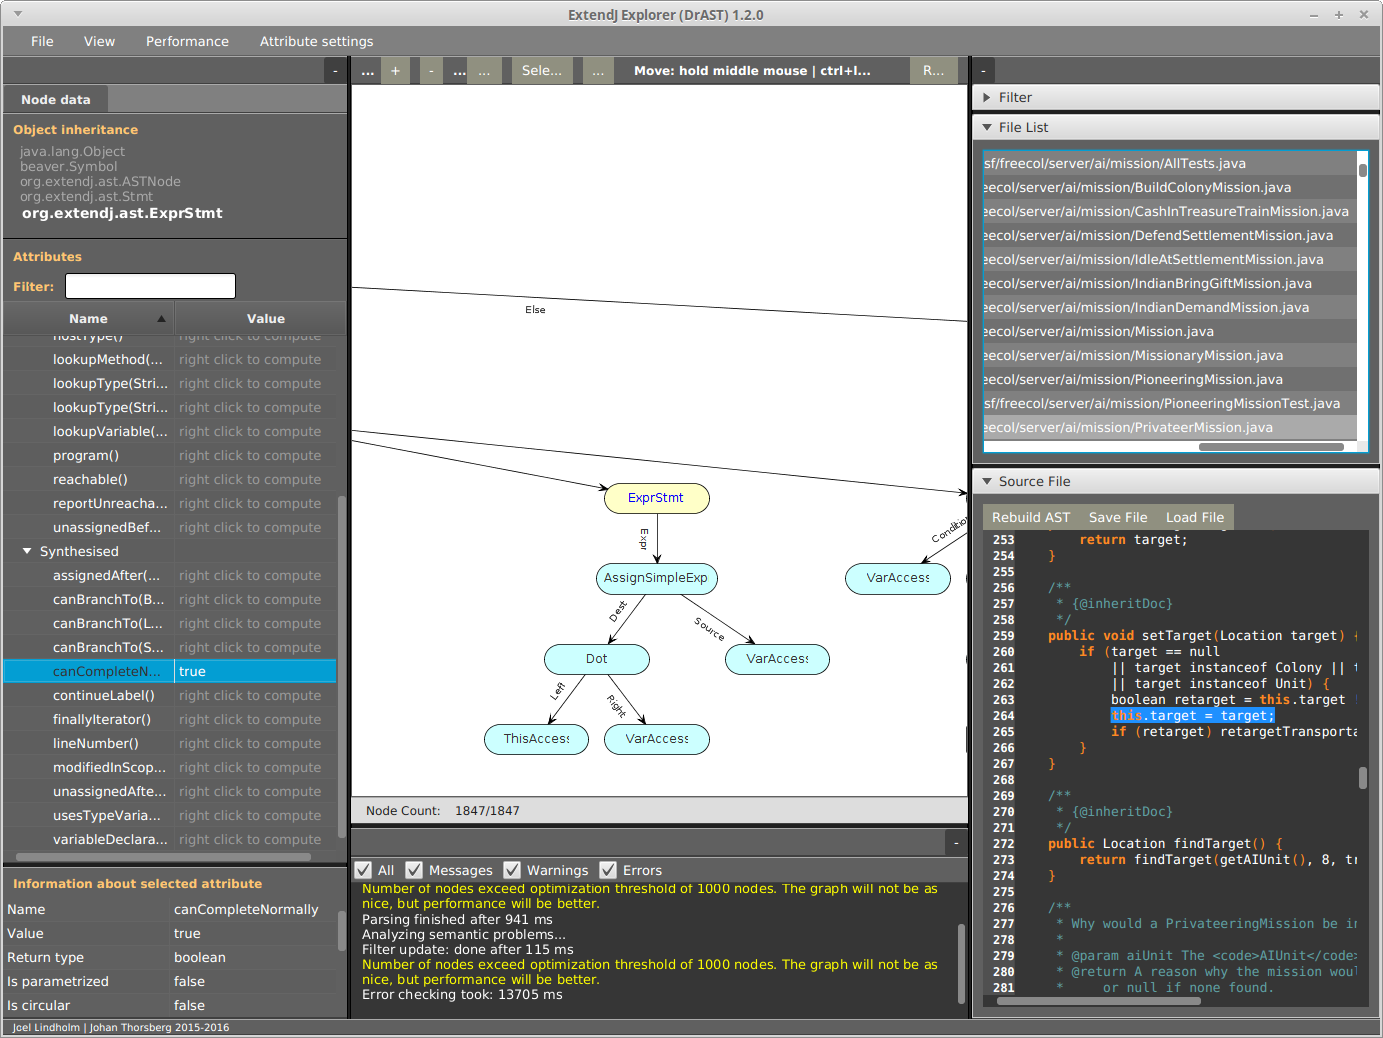
\includegraphics[width=1.0\textwidth]{figures/drast}
  \caption{
    Screenshot of DrAST extended with ExtendJ.
    The center part of the window contains a graph of the AST of one source file in
    freecol-0.10.7.
    The left part of the window contains a list of all attributes in the currently
    selected node. The \texttt{canCompleteNormally()} attribute has been selected and manually
    computed by the user.
    The right side of the window contains a list of all files in freecol-0.10.7,
    and below that is a source file view of the currently selected file.
    The bottom center part of the window shows status messages from DrAST. Note the
    message about compile-time error checking at the end.
    No compile-time errors or warnings were present in freecol-0.10.7.
  }
  \label{fig:screenshot1}
\end{figure}
\end{minipage}

}

\fi

\part[Popular Science Summary in Swedish]{\texorpdfstring{%
Popular Science Summary\\in Swedish}{%
Popular Science Summary in Swedish}}

\fi

\makeatletter
\def\@makeschapterhead#1{%
  \vspace*{10\p@}%
  {\parindent \z@ \raggedleft \reset@font
            \sffamily \bfseries \scshape \vphantom{\@chapapp{} \thechapter}
        \par\nobreak
        \interlinepenalty\@M
    \Huge  #1\par\nobreak
    \hrulefill
    \par\nobreak
    \vskip 16\p@
  }}
\makeatother

%\renewcommand{\figurename}{Figur}
\chapter*{Utveckling av statisk analys}

%Den här avhandlingen handlar om utveckling av \emph{statisk programanalys}.
\emph{Statisk programanalys}, eller kort och gott statisk analys,
är av stor betydelse inom mjukvaruutveckling.
Statisk analys är en samlingsterm för olika automatiserade analyser av datorprogram.
Framför allt behövs statisk analys för att kompilera program till exekverbar maskinkod,
så att de kan köras på en dator (eller mobiltelefon, till exempel).
Statisk analys används också för att hitta och förhindra fel i program,
samt för att optimera prestandan hos program.
Med statisk analys kan man bland annat hitta säkerhetshål och förhindra att känslig data läcker ut ur
ett program.
Dessutom används statisk analys i \emph{programmeringsverktyg}, alltså de verktyg en programmerare
använder för att konstruera sina program. Till exempel kan statisk analys användas för att
föreslå ändringar i koden (kodkomplettering och korrigering av enkla fel),
eller för att låta programmeraren snabbt hoppa mellan definitioner och användningar av
namn i koden.

\begin{center}
\scalebox{0.8}{
% http://www.texample.net/tikz/examples/pdca-cycle/
\definecolor{centerfill}{RGB}{108,80,190}
\definecolor{arrowfill}{RGB}{246,140,180}

\newcommand{\aarrow}[3]{%
   \pgfmathsetmacro{\astart}{#1}
   \pgfmathsetmacro{\aend}{#2}
   \pgfmathsetmacro{\atip}{5}
   \fill[arrowfill, very thick] (\astart+\atip:\rin)
                         arc (\astart+\atip:\aend:\rin)
      -- (\aend-\atip:\rmid)
      -- (\aend:\rout)   arc (\aend:\astart+\atip:\rout)
      -- (\astart:\rmid) -- cycle;
   \path[
      decorate,
      decoration={
        text along path,
        raise=-0.5ex,
        text={|\sffamily\footnotesize\bfseries|#3},
        text align={center}
      },
   ](\astart:\rmid) arc (\astart:\aend:\rmid);
}

\pgfmathsetmacro{\rin}{3.5}
\pgfmathsetmacro{\rmid}{4}
\pgfmathsetmacro{\rout}{4.5}

\begin{tikzpicture}[
	font={\sffamily},
  proc/.style={circle, align=center}
  ]
  \node[proc] at (180:\rmid) {
    
\includegraphics[width=2cm]{figures/doggo} \\
    programmering
  };
  \aarrow{150}{93}{källkod}
  \node[proc] at (60:\rmid) {
    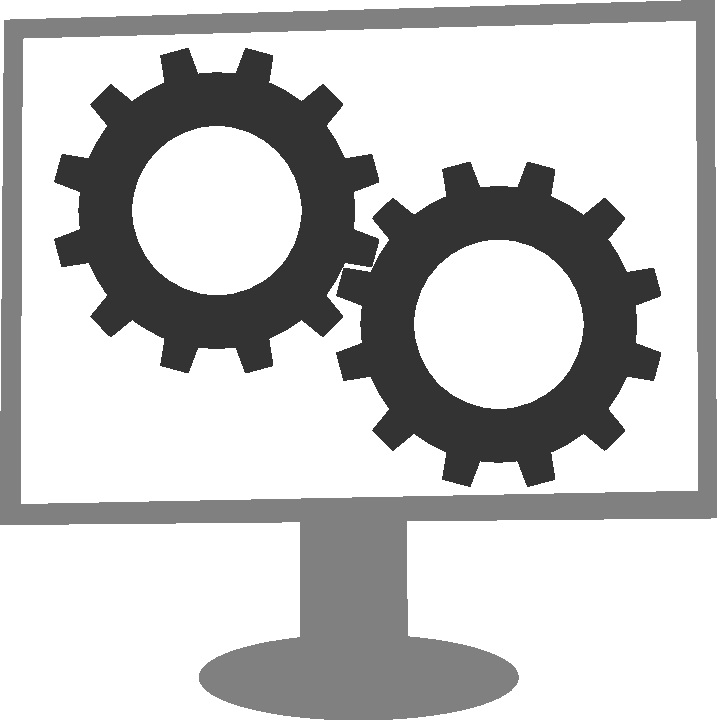
\includegraphics[width=1.5cm]{figures/compiler} \\
    kompilering \\
    \& analys
  };
  \aarrow{25}{-27}{exekverbart program}
  \node[proc] at (300:\rmid) {
    
\includegraphics[width=1.5cm]{figures/testing} \\
    testning
  };
  \aarrow{270}{210}{testresultat}
	\node[draw, circle, color=white, fill=centerfill,
		minimum width=4cm,
    align=center] at (0,0) {\sffamily\bfseries{}Utvecklingscykel\\för programvara};
\end{tikzpicture}
}
\end{center}
\noindent
\textbf{Figur:} Den vanliga utvecklingsprocessen för datorprogram.
Under programmering och kompilering används statisk analys av programmeraren och kompilatorn.

\vspace{1.5em}

Statisk analys är en form av mjukvara som ofta är komplicerad och tidskrävande att utveckla.
Dessutom finns det ofta ett behov av att kunna bygga vidare på en befintlig statisk analys med
nya egenskaper, till exempel om programmeringsspråket som analyseras uppdateras.
Således är det önskvärt att utveckla statisk analys med en flexibel mjukvaruarkitektur, det vill
säga på ett sätt som gör det möjligt att bygga på analysen utan allt för stor ansträngning.

Givet att det finns några grundläggande analyser som är utvecklade
med flexibel arkitektur så kan vi utveckla många nya viktiga analyser som använder de grundläggande
analyserna som byggstenar. Detta sparar mycket tid och pengar.

\subsection*{Deklarativ programmering}

För att uppnå en flexibel mjukvaruarkitektur kan vi använda oss av \emph{deklarativ programmering}.
Det innebär att programmeraren beskriver \emph{vad} som skall beräknas, snarare än
att exakt beskriva stegen som datorn tar för att beräkna det som behövs.
Den främsta fördelen med
deklarativ programmering, när det gäller att bygga flexibla program, är att det blir enkelt
att dela upp ett deklarativt program i moduler.
Programmoduler kan utvecklas separat och sedan kombineras på olika sätt, vilket sparar tid
för programmerarna i det långa loppet.
En deklarativ statisk analys kan ganska enkelt användas som en modul inuti en större, mer komplicerad,
analys.

En statisk analys kan delas upp i små deklarativa delar som kallas
\emph{attribut}. Attributen kan enkelt kombineras till moduler som sedan
används för att utveckla nya analyser.

Ett sätt att tänka på modulerna i en statisk analys är som pusselbitar. En pusselbit (modul)
kan läggas till i ett pussel (en statisk analys) så länge den har rätt form (programgränssnitt):

\begin{center}

\includegraphics[width=4cm]{figures/puzzle}
\end{center}

\vspace{1em}

Ett viktigt forskningsresultat i den här avhandlingen är en ny algoritm för att kunna beräkna
flera attribut samtidigt. Detta kan förkorta beräkningstiden: i ett experiment visade mina
mätningar att kompileringstiden kunde kortas med hälften.
En annan fördel är att svarstiden kan minskas i interaktiva
programmeringsverktyg: med samtidiga beräkningar måste man inte vänta på att föregående beräkningar
är klara innan man börjar på den nästa. Mina experimentella resultat visar att svarstiden kan minskas
från sekunder till under en millisekund.

\newpage
För att kunna utföra beräkningar samtidigt har de flesta datorer idag flera
\emph{kärnor}, där varje kärna exekverar varsin \emph{beräkningstråd}
jämnlöpande med andra kärnor i datorn.
Med min nya algoritm kan den sammanlagda beräkningstiden för attribut minskas genom att dela upp
beräkningsarbetet på flera (beräknings)trådar.
När en tråd beräknat ett attribut sparas värdet och kan direkt användas av en efterföljande tråd
som då slipper göra om beräkningsarbetet.
Uppdelning av arbetet för fem attribut med två jämnlöpande trådar illustreras i figuren nedan.

\begin{center}
\begin{tikzpicture}[
    >={Triangle[angle=45:6pt,length=6pt]},
    every node/.style={draw, ellipse},
    every join/.style={->},
    state/.style={pattern=north east lines}]
  \node[state] (R) {};
  \node[state, below=of R] (C) {};
  \node[state, below left=of C] (D) {};
  \node[state, below right=of C] (E) {};
  \node[state, left=of D] (R1) {};
  \node[above=of R1, color=red] (T1) {$T_1$};
  \node[right =of R, color=blue] (T2) {$T_2$};
  \draw[->,color=red]
      (T1) edge (R1)
      (R1) edge (D)
      (D) edge [bend left] (C)
      (C) edge [bend left] (E)
      (E) edge [bend left] (D);
  \path[every edge/.style={
      draw, ->, color=blue,
      decorate,
      decoration={
        snake,
        amplitude=0.8mm,
        segment length=4.1mm,
        pre length=0.8mm,
        post length=2mm}
      }]
      (T2) edge  (R)
      (R) edge  (C)
      (C) edge  (E)
      (E) edge  (D)
      (D) edge  (C);
\end{tikzpicture}
\end{center}

\noindent
\textbf{Figur:} Illustration av två trådar, $T_1$ och $T_2$, som samtidigt beräknar fem
attribut (randiga cirklar).
Beräkningsflödet för $T_1$ visas med röda pilar,
och för $T_2$ med vågiga blåa pilar.
Beräkningen är i det här fallet \emph{iterativ}, och går runt i en cirkel tills det rätta värdet har
beräknats.
Med min algoritm kan varje tråd utföra sin beräkning i varje attribut utan att
behöva vänta på den andra tråden. Dessutom hjälper trådarna varandra genom att en tråd använder
resultatet från den andra tråden om den andra hann före.

\subsection*{Kompilatorer}

Statiska analyser är centrala i kompilatorer, det vill säga program som översätter programmerarens
kod till maskinkod som en dator kan köra.
I mitt arbete har jag arbetat främst med en kompilator som heter ExtendJ, som
kompilerar program skrivna i programmeringsspråket Java. ExtendJ är fullt deklarativt
programmerad och använder attribut, vilket gör det förhållandevis enkelt att använda ExtendJ för att
bygga nya statiska analyser för Java.

För min avhandling har jag
dels utvecklat nya analyser som bygger på ExtendJ,
dels förbättrat ExtendJ självt.

Bland de statiska analyser som jag utvecklat i ExtendJ finns en analys som kan användas
för att minska testningstiden för Java-program. Idén är att endast köra om de test som kan påverkas av
den senaste ändringen i programmet som testas.
Med denna teknik lyckades jag halvera den totala tiden för testning av
flera olika program.

En av förbättringarna jag gjort i ExtendJ var att uppdatera kompilatorn till att
stödja en ny version av Java.  Sammanlagt har förbättringarna som jag gjort i
ExtendJ gjort det enklare för forskargrupper runt hela världen att bygga nya
statiska analyser och språktillägg till Java.

\end{document}

